% !TeX root = ../main.tex
% !TeX encoding = UTF-8
% !TeX spellcheck = it-IT
% !TeX program = xelatex

\section{Introduzione}
\begin{frame}{Normali climatiche: un'istantanea di trent'anni}
  Le normali climatiche sono la sintesi dei dati meteorologici di un determinato trentennio
  \begin{figure}
    \centering
    \begin{subtable}[m]{0.3\textwidth}
      \centering
      \small
      
\begin{tabular}[t]{ll}
  \toprule
  Stazione & Firenzuola\\
  Longitudine & 11.37465\\
  Latitudine & 44.12201\\
  Quota & 476\\
  Data & \DTMDisplaydate{2004}{10}{05}{-1}\\
  tmin & \qty{12.3}{\degreeCelsius}\\
  tmax & \qty{23.9}{\degreeCelsius}\\
  \bottomrule
\end{tabular}
      \caption{Esempio di dato grezzo}
    \end{subtable}
    \hfill
    \begin{subfigure}[m]{0.3\textwidth}
      \centering
      % Created by tikzDevice version 0.12.6 on 2025-04-06 18:10:19
% !TEX encoding = UTF-8 Unicode
\begin{tikzpicture}[x=1pt,y=1pt]
  \definecolor{fillColor}{RGB}{255,255,255}
  \path[use as bounding box,fill=fillColor] (0,0) rectangle (113.81, 93.89);
  \begin{scope}
    \path[clip] (  0.00,  3.21) rectangle (113.81, 90.69);
    \definecolor{drawColor}{RGB}{255,255,255}

    \path[draw=drawColor,line width= 0.6pt,line join=round,line cap=round,fill=fillColor] (  0.00,  3.21) rectangle (113.81, 90.69);
  \end{scope}
  \begin{scope}
    \path[clip] (  8.25, 11.46) rectangle ( 88.54, 85.19);
    \definecolor{fillColor}{RGB}{255,255,255}

    \path[fill=fillColor] (  8.25, 11.46) rectangle ( 88.54, 85.19);
    \definecolor{drawColor}{gray}{0.92}

    \path[draw=drawColor,line width= 0.6pt,line join=round,line cap=round] ( 15.08, 11.46) --
    ( 15.08, 11.79) --
    ( 15.08, 12.65) --
    ( 15.08, 13.51) --
    ( 15.08, 14.38) --
    ( 15.08, 15.24) --
    ( 15.08, 16.10) --
    ( 15.08, 16.97) --
    ( 15.08, 17.83) --
    ( 15.08, 18.70) --
    ( 15.08, 19.56) --
    ( 15.08, 20.42) --
    ( 15.08, 21.29) --
    ( 15.08, 22.15) --
    ( 15.08, 23.01) --
    ( 15.08, 23.88) --
    ( 15.08, 24.74) --
    ( 15.08, 25.61) --
    ( 15.08, 26.47) --
    ( 15.08, 27.33) --
    ( 15.08, 28.20) --
    ( 15.08, 29.06) --
    ( 15.08, 29.92) --
    ( 15.08, 30.79) --
    ( 15.08, 31.65) --
    ( 15.08, 32.52) --
    ( 15.08, 33.38) --
    ( 15.08, 34.24) --
    ( 15.08, 35.11) --
    ( 15.08, 35.97) --
    ( 15.08, 36.83) --
    ( 15.08, 37.70) --
    ( 15.08, 38.56) --
    ( 15.08, 39.42) --
    ( 15.08, 40.29) --
    ( 15.08, 41.15) --
    ( 15.08, 42.02) --
    ( 15.08, 42.88) --
    ( 15.08, 43.74) --
    ( 15.08, 44.61) --
    ( 15.08, 45.47) --
    ( 15.08, 46.33) --
    ( 15.08, 47.20) --
    ( 15.08, 48.06) --
    ( 15.08, 48.93) --
    ( 15.08, 49.79) --
    ( 15.08, 50.65) --
    ( 15.08, 51.52) --
    ( 15.08, 52.38) --
    ( 15.08, 53.24) --
    ( 15.08, 54.11) --
    ( 15.08, 54.97) --
    ( 15.08, 55.84) --
    ( 15.08, 56.70) --
    ( 15.08, 57.56) --
    ( 15.08, 58.43) --
    ( 15.08, 59.29) --
    ( 15.08, 60.15) --
    ( 15.08, 61.02) --
    ( 15.08, 61.88) --
    ( 15.08, 62.75) --
    ( 15.08, 63.61) --
    ( 15.08, 64.47) --
    ( 15.08, 65.34) --
    ( 15.08, 66.20) --
    ( 15.08, 67.06) --
    ( 15.08, 67.93) --
    ( 15.08, 68.79) --
    ( 15.08, 69.66) --
    ( 15.08, 70.52) --
    ( 15.08, 71.38) --
    ( 15.08, 72.25) --
    ( 15.08, 73.11) --
    ( 15.08, 73.97) --
    ( 15.08, 74.84) --
    ( 15.08, 75.70) --
    ( 15.08, 76.57) --
    ( 15.08, 77.43) --
    ( 15.08, 78.29) --
    ( 15.08, 79.16) --
    ( 15.08, 80.02) --
    ( 15.08, 80.88) --
    ( 15.08, 81.75) --
    ( 15.08, 82.61) --
    ( 15.08, 83.47) --
    ( 15.08, 84.34) --
    ( 15.08, 85.19);

    \path[draw=drawColor,line width= 0.6pt,line join=round,line cap=round] ( 25.22, 11.46) --
    ( 25.22, 11.79) --
    ( 25.22, 12.65) --
    ( 25.22, 13.51) --
    ( 25.22, 14.38) --
    ( 25.22, 15.24) --
    ( 25.22, 16.10) --
    ( 25.22, 16.97) --
    ( 25.22, 17.83) --
    ( 25.22, 18.70) --
    ( 25.22, 19.56) --
    ( 25.22, 20.42) --
    ( 25.22, 21.29) --
    ( 25.22, 22.15) --
    ( 25.22, 23.01) --
    ( 25.22, 23.88) --
    ( 25.22, 24.74) --
    ( 25.22, 25.61) --
    ( 25.22, 26.47) --
    ( 25.22, 27.33) --
    ( 25.22, 28.20) --
    ( 25.22, 29.06) --
    ( 25.22, 29.92) --
    ( 25.22, 30.79) --
    ( 25.22, 31.65) --
    ( 25.22, 32.52) --
    ( 25.22, 33.38) --
    ( 25.22, 34.24) --
    ( 25.22, 35.11) --
    ( 25.22, 35.97) --
    ( 25.22, 36.83) --
    ( 25.22, 37.70) --
    ( 25.22, 38.56) --
    ( 25.22, 39.42) --
    ( 25.22, 40.29) --
    ( 25.22, 41.15) --
    ( 25.22, 42.02) --
    ( 25.22, 42.88) --
    ( 25.22, 43.74) --
    ( 25.22, 44.61) --
    ( 25.22, 45.47) --
    ( 25.22, 46.33) --
    ( 25.22, 47.20) --
    ( 25.22, 48.06) --
    ( 25.22, 48.93) --
    ( 25.22, 49.79) --
    ( 25.22, 50.65) --
    ( 25.22, 51.52) --
    ( 25.22, 52.38) --
    ( 25.22, 53.24) --
    ( 25.22, 54.11) --
    ( 25.22, 54.97) --
    ( 25.22, 55.84) --
    ( 25.22, 56.70) --
    ( 25.22, 57.56) --
    ( 25.22, 58.43) --
    ( 25.22, 59.29) --
    ( 25.22, 60.15) --
    ( 25.22, 61.02) --
    ( 25.22, 61.88) --
    ( 25.22, 62.75) --
    ( 25.22, 63.61) --
    ( 25.22, 64.47) --
    ( 25.22, 65.34) --
    ( 25.22, 66.20) --
    ( 25.22, 67.06) --
    ( 25.22, 67.93) --
    ( 25.22, 68.79) --
    ( 25.22, 69.66) --
    ( 25.22, 70.52) --
    ( 25.22, 71.38) --
    ( 25.22, 72.25) --
    ( 25.22, 73.11) --
    ( 25.22, 73.97) --
    ( 25.22, 74.84) --
    ( 25.22, 75.70) --
    ( 25.22, 76.57) --
    ( 25.22, 77.43) --
    ( 25.22, 78.29) --
    ( 25.22, 79.16) --
    ( 25.22, 80.02) --
    ( 25.22, 80.88) --
    ( 25.22, 81.75) --
    ( 25.22, 82.61) --
    ( 25.22, 83.47) --
    ( 25.22, 84.34) --
    ( 25.22, 85.19);

    \path[draw=drawColor,line width= 0.6pt,line join=round,line cap=round] ( 35.35, 11.46) --
    ( 35.35, 11.79) --
    ( 35.35, 12.65) --
    ( 35.35, 13.51) --
    ( 35.35, 14.38) --
    ( 35.35, 15.24) --
    ( 35.35, 16.10) --
    ( 35.35, 16.97) --
    ( 35.35, 17.83) --
    ( 35.35, 18.70) --
    ( 35.35, 19.56) --
    ( 35.35, 20.42) --
    ( 35.35, 21.29) --
    ( 35.35, 22.15) --
    ( 35.35, 23.01) --
    ( 35.35, 23.88) --
    ( 35.35, 24.74) --
    ( 35.35, 25.61) --
    ( 35.35, 26.47) --
    ( 35.35, 27.33) --
    ( 35.35, 28.20) --
    ( 35.35, 29.06) --
    ( 35.35, 29.92) --
    ( 35.35, 30.79) --
    ( 35.35, 31.65) --
    ( 35.35, 32.52) --
    ( 35.35, 33.38) --
    ( 35.35, 34.24) --
    ( 35.35, 35.11) --
    ( 35.35, 35.97) --
    ( 35.35, 36.83) --
    ( 35.35, 37.70) --
    ( 35.35, 38.56) --
    ( 35.35, 39.42) --
    ( 35.35, 40.29) --
    ( 35.35, 41.15) --
    ( 35.35, 42.02) --
    ( 35.35, 42.88) --
    ( 35.35, 43.74) --
    ( 35.35, 44.61) --
    ( 35.35, 45.47) --
    ( 35.35, 46.33) --
    ( 35.35, 47.20) --
    ( 35.35, 48.06) --
    ( 35.35, 48.93) --
    ( 35.35, 49.79) --
    ( 35.35, 50.65) --
    ( 35.35, 51.52) --
    ( 35.35, 52.38) --
    ( 35.35, 53.24) --
    ( 35.35, 54.11) --
    ( 35.35, 54.97) --
    ( 35.35, 55.84) --
    ( 35.35, 56.70) --
    ( 35.35, 57.56) --
    ( 35.35, 58.43) --
    ( 35.35, 59.29) --
    ( 35.35, 60.15) --
    ( 35.35, 61.02) --
    ( 35.35, 61.88) --
    ( 35.35, 62.75) --
    ( 35.35, 63.61) --
    ( 35.35, 64.47) --
    ( 35.35, 65.34) --
    ( 35.35, 66.20) --
    ( 35.35, 67.06) --
    ( 35.35, 67.93) --
    ( 35.35, 68.79) --
    ( 35.35, 69.66) --
    ( 35.35, 70.52) --
    ( 35.35, 71.38) --
    ( 35.35, 72.25) --
    ( 35.35, 73.11) --
    ( 35.35, 73.97) --
    ( 35.35, 74.84) --
    ( 35.35, 75.70) --
    ( 35.35, 76.57) --
    ( 35.35, 77.43) --
    ( 35.35, 78.29) --
    ( 35.35, 79.16) --
    ( 35.35, 80.02) --
    ( 35.35, 80.88) --
    ( 35.35, 81.75) --
    ( 35.35, 82.61) --
    ( 35.35, 83.47) --
    ( 35.35, 84.34) --
    ( 35.35, 85.19);

    \path[draw=drawColor,line width= 0.6pt,line join=round,line cap=round] ( 45.48, 11.46) --
    ( 45.48, 11.79) --
    ( 45.48, 12.65) --
    ( 45.48, 13.51) --
    ( 45.48, 14.38) --
    ( 45.48, 15.24) --
    ( 45.48, 16.10) --
    ( 45.48, 16.97) --
    ( 45.48, 17.83) --
    ( 45.48, 18.70) --
    ( 45.48, 19.56) --
    ( 45.48, 20.42) --
    ( 45.48, 21.29) --
    ( 45.48, 22.15) --
    ( 45.48, 23.01) --
    ( 45.48, 23.88) --
    ( 45.48, 24.74) --
    ( 45.48, 25.61) --
    ( 45.48, 26.47) --
    ( 45.48, 27.33) --
    ( 45.48, 28.20) --
    ( 45.48, 29.06) --
    ( 45.48, 29.92) --
    ( 45.48, 30.79) --
    ( 45.48, 31.65) --
    ( 45.48, 32.52) --
    ( 45.48, 33.38) --
    ( 45.48, 34.24) --
    ( 45.48, 35.11) --
    ( 45.48, 35.97) --
    ( 45.48, 36.83) --
    ( 45.48, 37.70) --
    ( 45.48, 38.56) --
    ( 45.48, 39.42) --
    ( 45.48, 40.29) --
    ( 45.48, 41.15) --
    ( 45.48, 42.02) --
    ( 45.48, 42.88) --
    ( 45.48, 43.74) --
    ( 45.48, 44.61) --
    ( 45.48, 45.47) --
    ( 45.48, 46.33) --
    ( 45.48, 47.20) --
    ( 45.48, 48.06) --
    ( 45.48, 48.93) --
    ( 45.48, 49.79) --
    ( 45.48, 50.65) --
    ( 45.48, 51.52) --
    ( 45.48, 52.38) --
    ( 45.48, 53.24) --
    ( 45.48, 54.11) --
    ( 45.48, 54.97) --
    ( 45.48, 55.84) --
    ( 45.48, 56.70) --
    ( 45.48, 57.56) --
    ( 45.48, 58.43) --
    ( 45.48, 59.29) --
    ( 45.48, 60.15) --
    ( 45.48, 61.02) --
    ( 45.48, 61.88) --
    ( 45.48, 62.75) --
    ( 45.48, 63.61) --
    ( 45.48, 64.47) --
    ( 45.48, 65.34) --
    ( 45.48, 66.20) --
    ( 45.48, 67.06) --
    ( 45.48, 67.93) --
    ( 45.48, 68.79) --
    ( 45.48, 69.66) --
    ( 45.48, 70.52) --
    ( 45.48, 71.38) --
    ( 45.48, 72.25) --
    ( 45.48, 73.11) --
    ( 45.48, 73.97) --
    ( 45.48, 74.84) --
    ( 45.48, 75.70) --
    ( 45.48, 76.57) --
    ( 45.48, 77.43) --
    ( 45.48, 78.29) --
    ( 45.48, 79.16) --
    ( 45.48, 80.02) --
    ( 45.48, 80.88) --
    ( 45.48, 81.75) --
    ( 45.48, 82.61) --
    ( 45.48, 83.47) --
    ( 45.48, 84.34) --
    ( 45.48, 85.19);

    \path[draw=drawColor,line width= 0.6pt,line join=round,line cap=round] ( 55.61, 11.46) --
    ( 55.61, 11.79) --
    ( 55.61, 12.65) --
    ( 55.61, 13.51) --
    ( 55.61, 14.38) --
    ( 55.61, 15.24) --
    ( 55.61, 16.10) --
    ( 55.61, 16.97) --
    ( 55.61, 17.83) --
    ( 55.61, 18.70) --
    ( 55.61, 19.56) --
    ( 55.61, 20.42) --
    ( 55.61, 21.29) --
    ( 55.61, 22.15) --
    ( 55.61, 23.01) --
    ( 55.61, 23.88) --
    ( 55.61, 24.74) --
    ( 55.61, 25.61) --
    ( 55.61, 26.47) --
    ( 55.61, 27.33) --
    ( 55.61, 28.20) --
    ( 55.61, 29.06) --
    ( 55.61, 29.92) --
    ( 55.61, 30.79) --
    ( 55.61, 31.65) --
    ( 55.61, 32.52) --
    ( 55.61, 33.38) --
    ( 55.61, 34.24) --
    ( 55.61, 35.11) --
    ( 55.61, 35.97) --
    ( 55.61, 36.83) --
    ( 55.61, 37.70) --
    ( 55.61, 38.56) --
    ( 55.61, 39.42) --
    ( 55.61, 40.29) --
    ( 55.61, 41.15) --
    ( 55.61, 42.02) --
    ( 55.61, 42.88) --
    ( 55.61, 43.74) --
    ( 55.61, 44.61) --
    ( 55.61, 45.47) --
    ( 55.61, 46.33) --
    ( 55.61, 47.20) --
    ( 55.61, 48.06) --
    ( 55.61, 48.93) --
    ( 55.61, 49.79) --
    ( 55.61, 50.65) --
    ( 55.61, 51.52) --
    ( 55.61, 52.38) --
    ( 55.61, 53.24) --
    ( 55.61, 54.11) --
    ( 55.61, 54.97) --
    ( 55.61, 55.84) --
    ( 55.61, 56.70) --
    ( 55.61, 57.56) --
    ( 55.61, 58.43) --
    ( 55.61, 59.29) --
    ( 55.61, 60.15) --
    ( 55.61, 61.02) --
    ( 55.61, 61.88) --
    ( 55.61, 62.75) --
    ( 55.61, 63.61) --
    ( 55.61, 64.47) --
    ( 55.61, 65.34) --
    ( 55.61, 66.20) --
    ( 55.61, 67.06) --
    ( 55.61, 67.93) --
    ( 55.61, 68.79) --
    ( 55.61, 69.66) --
    ( 55.61, 70.52) --
    ( 55.61, 71.38) --
    ( 55.61, 72.25) --
    ( 55.61, 73.11) --
    ( 55.61, 73.97) --
    ( 55.61, 74.84) --
    ( 55.61, 75.70) --
    ( 55.61, 76.57) --
    ( 55.61, 77.43) --
    ( 55.61, 78.29) --
    ( 55.61, 79.16) --
    ( 55.61, 80.02) --
    ( 55.61, 80.88) --
    ( 55.61, 81.75) --
    ( 55.61, 82.61) --
    ( 55.61, 83.47) --
    ( 55.61, 84.34) --
    ( 55.61, 85.19);

    \path[draw=drawColor,line width= 0.6pt,line join=round,line cap=round] ( 65.75, 11.46) --
    ( 65.75, 11.79) --
    ( 65.75, 12.65) --
    ( 65.75, 13.51) --
    ( 65.75, 14.38) --
    ( 65.75, 15.24) --
    ( 65.75, 16.10) --
    ( 65.75, 16.97) --
    ( 65.75, 17.83) --
    ( 65.75, 18.70) --
    ( 65.75, 19.56) --
    ( 65.75, 20.42) --
    ( 65.75, 21.29) --
    ( 65.75, 22.15) --
    ( 65.75, 23.01) --
    ( 65.75, 23.88) --
    ( 65.75, 24.74) --
    ( 65.75, 25.61) --
    ( 65.75, 26.47) --
    ( 65.75, 27.33) --
    ( 65.75, 28.20) --
    ( 65.75, 29.06) --
    ( 65.75, 29.92) --
    ( 65.75, 30.79) --
    ( 65.75, 31.65) --
    ( 65.75, 32.52) --
    ( 65.75, 33.38) --
    ( 65.75, 34.24) --
    ( 65.75, 35.11) --
    ( 65.75, 35.97) --
    ( 65.75, 36.83) --
    ( 65.75, 37.70) --
    ( 65.75, 38.56) --
    ( 65.75, 39.42) --
    ( 65.75, 40.29) --
    ( 65.75, 41.15) --
    ( 65.75, 42.02) --
    ( 65.75, 42.88) --
    ( 65.75, 43.74) --
    ( 65.75, 44.61) --
    ( 65.75, 45.47) --
    ( 65.75, 46.33) --
    ( 65.75, 47.20) --
    ( 65.75, 48.06) --
    ( 65.75, 48.93) --
    ( 65.75, 49.79) --
    ( 65.75, 50.65) --
    ( 65.75, 51.52) --
    ( 65.75, 52.38) --
    ( 65.75, 53.24) --
    ( 65.75, 54.11) --
    ( 65.75, 54.97) --
    ( 65.75, 55.84) --
    ( 65.75, 56.70) --
    ( 65.75, 57.56) --
    ( 65.75, 58.43) --
    ( 65.75, 59.29) --
    ( 65.75, 60.15) --
    ( 65.75, 61.02) --
    ( 65.75, 61.88) --
    ( 65.75, 62.75) --
    ( 65.75, 63.61) --
    ( 65.75, 64.47) --
    ( 65.75, 65.34) --
    ( 65.75, 66.20) --
    ( 65.75, 67.06) --
    ( 65.75, 67.93) --
    ( 65.75, 68.79) --
    ( 65.75, 69.66) --
    ( 65.75, 70.52) --
    ( 65.75, 71.38) --
    ( 65.75, 72.25) --
    ( 65.75, 73.11) --
    ( 65.75, 73.97) --
    ( 65.75, 74.84) --
    ( 65.75, 75.70) --
    ( 65.75, 76.57) --
    ( 65.75, 77.43) --
    ( 65.75, 78.29) --
    ( 65.75, 79.16) --
    ( 65.75, 80.02) --
    ( 65.75, 80.88) --
    ( 65.75, 81.75) --
    ( 65.75, 82.61) --
    ( 65.75, 83.47) --
    ( 65.75, 84.34) --
    ( 65.75, 85.19);

    \path[draw=drawColor,line width= 0.6pt,line join=round,line cap=round] ( 75.88, 11.46) --
    ( 75.88, 11.79) --
    ( 75.88, 12.65) --
    ( 75.88, 13.51) --
    ( 75.88, 14.38) --
    ( 75.88, 15.24) --
    ( 75.88, 16.10) --
    ( 75.88, 16.97) --
    ( 75.88, 17.83) --
    ( 75.88, 18.70) --
    ( 75.88, 19.56) --
    ( 75.88, 20.42) --
    ( 75.88, 21.29) --
    ( 75.88, 22.15) --
    ( 75.88, 23.01) --
    ( 75.88, 23.88) --
    ( 75.88, 24.74) --
    ( 75.88, 25.61) --
    ( 75.88, 26.47) --
    ( 75.88, 27.33) --
    ( 75.88, 28.20) --
    ( 75.88, 29.06) --
    ( 75.88, 29.92) --
    ( 75.88, 30.79) --
    ( 75.88, 31.65) --
    ( 75.88, 32.52) --
    ( 75.88, 33.38) --
    ( 75.88, 34.24) --
    ( 75.88, 35.11) --
    ( 75.88, 35.97) --
    ( 75.88, 36.83) --
    ( 75.88, 37.70) --
    ( 75.88, 38.56) --
    ( 75.88, 39.42) --
    ( 75.88, 40.29) --
    ( 75.88, 41.15) --
    ( 75.88, 42.02) --
    ( 75.88, 42.88) --
    ( 75.88, 43.74) --
    ( 75.88, 44.61) --
    ( 75.88, 45.47) --
    ( 75.88, 46.33) --
    ( 75.88, 47.20) --
    ( 75.88, 48.06) --
    ( 75.88, 48.93) --
    ( 75.88, 49.79) --
    ( 75.88, 50.65) --
    ( 75.88, 51.52) --
    ( 75.88, 52.38) --
    ( 75.88, 53.24) --
    ( 75.88, 54.11) --
    ( 75.88, 54.97) --
    ( 75.88, 55.84) --
    ( 75.88, 56.70) --
    ( 75.88, 57.56) --
    ( 75.88, 58.43) --
    ( 75.88, 59.29) --
    ( 75.88, 60.15) --
    ( 75.88, 61.02) --
    ( 75.88, 61.88) --
    ( 75.88, 62.75) --
    ( 75.88, 63.61) --
    ( 75.88, 64.47) --
    ( 75.88, 65.34) --
    ( 75.88, 66.20) --
    ( 75.88, 67.06) --
    ( 75.88, 67.93) --
    ( 75.88, 68.79) --
    ( 75.88, 69.66) --
    ( 75.88, 70.52) --
    ( 75.88, 71.38) --
    ( 75.88, 72.25) --
    ( 75.88, 73.11) --
    ( 75.88, 73.97) --
    ( 75.88, 74.84) --
    ( 75.88, 75.70) --
    ( 75.88, 76.57) --
    ( 75.88, 77.43) --
    ( 75.88, 78.29) --
    ( 75.88, 79.16) --
    ( 75.88, 80.02) --
    ( 75.88, 80.88) --
    ( 75.88, 81.75) --
    ( 75.88, 82.61) --
    ( 75.88, 83.47) --
    ( 75.88, 84.34) --
    ( 75.88, 85.19);

    \path[draw=drawColor,line width= 0.6pt,line join=round,line cap=round] ( 86.01, 11.46) --
    ( 86.01, 11.79) --
    ( 86.01, 12.65) --
    ( 86.01, 13.51) --
    ( 86.01, 14.38) --
    ( 86.01, 15.24) --
    ( 86.01, 16.10) --
    ( 86.01, 16.97) --
    ( 86.01, 17.83) --
    ( 86.01, 18.70) --
    ( 86.01, 19.56) --
    ( 86.01, 20.42) --
    ( 86.01, 21.29) --
    ( 86.01, 22.15) --
    ( 86.01, 23.01) --
    ( 86.01, 23.88) --
    ( 86.01, 24.74) --
    ( 86.01, 25.61) --
    ( 86.01, 26.47) --
    ( 86.01, 27.33) --
    ( 86.01, 28.20) --
    ( 86.01, 29.06) --
    ( 86.01, 29.92) --
    ( 86.01, 30.79) --
    ( 86.01, 31.65) --
    ( 86.01, 32.52) --
    ( 86.01, 33.38) --
    ( 86.01, 34.24) --
    ( 86.01, 35.11) --
    ( 86.01, 35.97) --
    ( 86.01, 36.83) --
    ( 86.01, 37.70) --
    ( 86.01, 38.56) --
    ( 86.01, 39.42) --
    ( 86.01, 40.29) --
    ( 86.01, 41.15) --
    ( 86.01, 42.02) --
    ( 86.01, 42.88) --
    ( 86.01, 43.74) --
    ( 86.01, 44.61) --
    ( 86.01, 45.47) --
    ( 86.01, 46.33) --
    ( 86.01, 47.20) --
    ( 86.01, 48.06) --
    ( 86.01, 48.93) --
    ( 86.01, 49.79) --
    ( 86.01, 50.65) --
    ( 86.01, 51.52) --
    ( 86.01, 52.38) --
    ( 86.01, 53.24) --
    ( 86.01, 54.11) --
    ( 86.01, 54.97) --
    ( 86.01, 55.84) --
    ( 86.01, 56.70) --
    ( 86.01, 57.56) --
    ( 86.01, 58.43) --
    ( 86.01, 59.29) --
    ( 86.01, 60.15) --
    ( 86.01, 61.02) --
    ( 86.01, 61.88) --
    ( 86.01, 62.75) --
    ( 86.01, 63.61) --
    ( 86.01, 64.47) --
    ( 86.01, 65.34) --
    ( 86.01, 66.20) --
    ( 86.01, 67.06) --
    ( 86.01, 67.93) --
    ( 86.01, 68.79) --
    ( 86.01, 69.66) --
    ( 86.01, 70.52) --
    ( 86.01, 71.38) --
    ( 86.01, 72.25) --
    ( 86.01, 73.11) --
    ( 86.01, 73.97) --
    ( 86.01, 74.84) --
    ( 86.01, 75.70) --
    ( 86.01, 76.57) --
    ( 86.01, 77.43) --
    ( 86.01, 78.29) --
    ( 86.01, 79.16) --
    ( 86.01, 80.02) --
    ( 86.01, 80.88) --
    ( 86.01, 81.75) --
    ( 86.01, 82.61) --
    ( 86.01, 83.47) --
    ( 86.01, 84.34) --
    ( 86.01, 85.19);

    \path[draw=drawColor,line width= 0.6pt,line join=round,line cap=round] (  8.25, 24.31) --
    (  8.63, 24.31) --
    (  9.56, 24.31) --
    ( 10.48, 24.31) --
    ( 11.40, 24.31) --
    ( 12.32, 24.31) --
    ( 13.24, 24.31) --
    ( 14.16, 24.31) --
    ( 15.08, 24.31) --
    ( 16.00, 24.31) --
    ( 16.93, 24.31) --
    ( 17.85, 24.31) --
    ( 18.77, 24.31) --
    ( 19.69, 24.31) --
    ( 20.61, 24.31) --
    ( 21.53, 24.31) --
    ( 22.45, 24.31) --
    ( 23.37, 24.31) --
    ( 24.29, 24.31) --
    ( 25.22, 24.31) --
    ( 26.14, 24.31) --
    ( 27.06, 24.31) --
    ( 27.98, 24.31) --
    ( 28.90, 24.31) --
    ( 29.82, 24.31) --
    ( 30.74, 24.31) --
    ( 31.66, 24.31) --
    ( 32.58, 24.31) --
    ( 33.51, 24.31) --
    ( 34.43, 24.31) --
    ( 35.35, 24.31) --
    ( 36.27, 24.31) --
    ( 37.19, 24.31) --
    ( 38.11, 24.31) --
    ( 39.03, 24.31) --
    ( 39.95, 24.31) --
    ( 40.87, 24.31) --
    ( 41.80, 24.31) --
    ( 42.72, 24.31) --
    ( 43.64, 24.31) --
    ( 44.56, 24.31) --
    ( 45.48, 24.31) --
    ( 46.40, 24.31) --
    ( 47.32, 24.31) --
    ( 48.24, 24.31) --
    ( 49.17, 24.31) --
    ( 50.09, 24.31) --
    ( 51.01, 24.31) --
    ( 51.93, 24.31) --
    ( 52.85, 24.31) --
    ( 53.77, 24.31) --
    ( 54.69, 24.31) --
    ( 55.61, 24.31) --
    ( 56.53, 24.31) --
    ( 57.46, 24.31) --
    ( 58.38, 24.31) --
    ( 59.30, 24.31) --
    ( 60.22, 24.31) --
    ( 61.14, 24.31) --
    ( 62.06, 24.31) --
    ( 62.98, 24.31) --
    ( 63.90, 24.31) --
    ( 64.82, 24.31) --
    ( 65.75, 24.31) --
    ( 66.67, 24.31) --
    ( 67.59, 24.31) --
    ( 68.51, 24.31) --
    ( 69.43, 24.31) --
    ( 70.35, 24.31) --
    ( 71.27, 24.31) --
    ( 72.19, 24.31) --
    ( 73.11, 24.31) --
    ( 74.04, 24.31) --
    ( 74.96, 24.31) --
    ( 75.88, 24.31) --
    ( 76.80, 24.31) --
    ( 77.72, 24.31) --
    ( 78.64, 24.31) --
    ( 79.56, 24.31) --
    ( 80.48, 24.31) --
    ( 81.41, 24.31) --
    ( 82.33, 24.31) --
    ( 83.25, 24.31) --
    ( 84.17, 24.31) --
    ( 85.09, 24.31) --
    ( 86.01, 24.31) --
    ( 86.93, 24.31) --
    ( 87.85, 24.31) --
    ( 88.54, 24.31);

    \path[draw=drawColor,line width= 0.6pt,line join=round,line cap=round] (  8.25, 38.56) --
    (  8.63, 38.56) --
    (  9.56, 38.56) --
    ( 10.48, 38.56) --
    ( 11.40, 38.56) --
    ( 12.32, 38.56) --
    ( 13.24, 38.56) --
    ( 14.16, 38.56) --
    ( 15.08, 38.56) --
    ( 16.00, 38.56) --
    ( 16.93, 38.56) --
    ( 17.85, 38.56) --
    ( 18.77, 38.56) --
    ( 19.69, 38.56) --
    ( 20.61, 38.56) --
    ( 21.53, 38.56) --
    ( 22.45, 38.56) --
    ( 23.37, 38.56) --
    ( 24.29, 38.56) --
    ( 25.22, 38.56) --
    ( 26.14, 38.56) --
    ( 27.06, 38.56) --
    ( 27.98, 38.56) --
    ( 28.90, 38.56) --
    ( 29.82, 38.56) --
    ( 30.74, 38.56) --
    ( 31.66, 38.56) --
    ( 32.58, 38.56) --
    ( 33.51, 38.56) --
    ( 34.43, 38.56) --
    ( 35.35, 38.56) --
    ( 36.27, 38.56) --
    ( 37.19, 38.56) --
    ( 38.11, 38.56) --
    ( 39.03, 38.56) --
    ( 39.95, 38.56) --
    ( 40.87, 38.56) --
    ( 41.80, 38.56) --
    ( 42.72, 38.56) --
    ( 43.64, 38.56) --
    ( 44.56, 38.56) --
    ( 45.48, 38.56) --
    ( 46.40, 38.56) --
    ( 47.32, 38.56) --
    ( 48.24, 38.56) --
    ( 49.17, 38.56) --
    ( 50.09, 38.56) --
    ( 51.01, 38.56) --
    ( 51.93, 38.56) --
    ( 52.85, 38.56) --
    ( 53.77, 38.56) --
    ( 54.69, 38.56) --
    ( 55.61, 38.56) --
    ( 56.53, 38.56) --
    ( 57.46, 38.56) --
    ( 58.38, 38.56) --
    ( 59.30, 38.56) --
    ( 60.22, 38.56) --
    ( 61.14, 38.56) --
    ( 62.06, 38.56) --
    ( 62.98, 38.56) --
    ( 63.90, 38.56) --
    ( 64.82, 38.56) --
    ( 65.75, 38.56) --
    ( 66.67, 38.56) --
    ( 67.59, 38.56) --
    ( 68.51, 38.56) --
    ( 69.43, 38.56) --
    ( 70.35, 38.56) --
    ( 71.27, 38.56) --
    ( 72.19, 38.56) --
    ( 73.11, 38.56) --
    ( 74.04, 38.56) --
    ( 74.96, 38.56) --
    ( 75.88, 38.56) --
    ( 76.80, 38.56) --
    ( 77.72, 38.56) --
    ( 78.64, 38.56) --
    ( 79.56, 38.56) --
    ( 80.48, 38.56) --
    ( 81.41, 38.56) --
    ( 82.33, 38.56) --
    ( 83.25, 38.56) --
    ( 84.17, 38.56) --
    ( 85.09, 38.56) --
    ( 86.01, 38.56) --
    ( 86.93, 38.56) --
    ( 87.85, 38.56) --
    ( 88.54, 38.56);

    \path[draw=drawColor,line width= 0.6pt,line join=round,line cap=round] (  8.25, 52.81) --
    (  8.63, 52.81) --
    (  9.56, 52.81) --
    ( 10.48, 52.81) --
    ( 11.40, 52.81) --
    ( 12.32, 52.81) --
    ( 13.24, 52.81) --
    ( 14.16, 52.81) --
    ( 15.08, 52.81) --
    ( 16.00, 52.81) --
    ( 16.93, 52.81) --
    ( 17.85, 52.81) --
    ( 18.77, 52.81) --
    ( 19.69, 52.81) --
    ( 20.61, 52.81) --
    ( 21.53, 52.81) --
    ( 22.45, 52.81) --
    ( 23.37, 52.81) --
    ( 24.29, 52.81) --
    ( 25.22, 52.81) --
    ( 26.14, 52.81) --
    ( 27.06, 52.81) --
    ( 27.98, 52.81) --
    ( 28.90, 52.81) --
    ( 29.82, 52.81) --
    ( 30.74, 52.81) --
    ( 31.66, 52.81) --
    ( 32.58, 52.81) --
    ( 33.51, 52.81) --
    ( 34.43, 52.81) --
    ( 35.35, 52.81) --
    ( 36.27, 52.81) --
    ( 37.19, 52.81) --
    ( 38.11, 52.81) --
    ( 39.03, 52.81) --
    ( 39.95, 52.81) --
    ( 40.87, 52.81) --
    ( 41.80, 52.81) --
    ( 42.72, 52.81) --
    ( 43.64, 52.81) --
    ( 44.56, 52.81) --
    ( 45.48, 52.81) --
    ( 46.40, 52.81) --
    ( 47.32, 52.81) --
    ( 48.24, 52.81) --
    ( 49.17, 52.81) --
    ( 50.09, 52.81) --
    ( 51.01, 52.81) --
    ( 51.93, 52.81) --
    ( 52.85, 52.81) --
    ( 53.77, 52.81) --
    ( 54.69, 52.81) --
    ( 55.61, 52.81) --
    ( 56.53, 52.81) --
    ( 57.46, 52.81) --
    ( 58.38, 52.81) --
    ( 59.30, 52.81) --
    ( 60.22, 52.81) --
    ( 61.14, 52.81) --
    ( 62.06, 52.81) --
    ( 62.98, 52.81) --
    ( 63.90, 52.81) --
    ( 64.82, 52.81) --
    ( 65.75, 52.81) --
    ( 66.67, 52.81) --
    ( 67.59, 52.81) --
    ( 68.51, 52.81) --
    ( 69.43, 52.81) --
    ( 70.35, 52.81) --
    ( 71.27, 52.81) --
    ( 72.19, 52.81) --
    ( 73.11, 52.81) --
    ( 74.04, 52.81) --
    ( 74.96, 52.81) --
    ( 75.88, 52.81) --
    ( 76.80, 52.81) --
    ( 77.72, 52.81) --
    ( 78.64, 52.81) --
    ( 79.56, 52.81) --
    ( 80.48, 52.81) --
    ( 81.41, 52.81) --
    ( 82.33, 52.81) --
    ( 83.25, 52.81) --
    ( 84.17, 52.81) --
    ( 85.09, 52.81) --
    ( 86.01, 52.81) --
    ( 86.93, 52.81) --
    ( 87.85, 52.81) --
    ( 88.54, 52.81);

    \path[draw=drawColor,line width= 0.6pt,line join=round,line cap=round] (  8.25, 67.06) --
    (  8.63, 67.06) --
    (  9.56, 67.06) --
    ( 10.48, 67.06) --
    ( 11.40, 67.06) --
    ( 12.32, 67.06) --
    ( 13.24, 67.06) --
    ( 14.16, 67.06) --
    ( 15.08, 67.06) --
    ( 16.00, 67.06) --
    ( 16.93, 67.06) --
    ( 17.85, 67.06) --
    ( 18.77, 67.06) --
    ( 19.69, 67.06) --
    ( 20.61, 67.06) --
    ( 21.53, 67.06) --
    ( 22.45, 67.06) --
    ( 23.37, 67.06) --
    ( 24.29, 67.06) --
    ( 25.22, 67.06) --
    ( 26.14, 67.06) --
    ( 27.06, 67.06) --
    ( 27.98, 67.06) --
    ( 28.90, 67.06) --
    ( 29.82, 67.06) --
    ( 30.74, 67.06) --
    ( 31.66, 67.06) --
    ( 32.58, 67.06) --
    ( 33.51, 67.06) --
    ( 34.43, 67.06) --
    ( 35.35, 67.06) --
    ( 36.27, 67.06) --
    ( 37.19, 67.06) --
    ( 38.11, 67.06) --
    ( 39.03, 67.06) --
    ( 39.95, 67.06) --
    ( 40.87, 67.06) --
    ( 41.80, 67.06) --
    ( 42.72, 67.06) --
    ( 43.64, 67.06) --
    ( 44.56, 67.06) --
    ( 45.48, 67.06) --
    ( 46.40, 67.06) --
    ( 47.32, 67.06) --
    ( 48.24, 67.06) --
    ( 49.17, 67.06) --
    ( 50.09, 67.06) --
    ( 51.01, 67.06) --
    ( 51.93, 67.06) --
    ( 52.85, 67.06) --
    ( 53.77, 67.06) --
    ( 54.69, 67.06) --
    ( 55.61, 67.06) --
    ( 56.53, 67.06) --
    ( 57.46, 67.06) --
    ( 58.38, 67.06) --
    ( 59.30, 67.06) --
    ( 60.22, 67.06) --
    ( 61.14, 67.06) --
    ( 62.06, 67.06) --
    ( 62.98, 67.06) --
    ( 63.90, 67.06) --
    ( 64.82, 67.06) --
    ( 65.75, 67.06) --
    ( 66.67, 67.06) --
    ( 67.59, 67.06) --
    ( 68.51, 67.06) --
    ( 69.43, 67.06) --
    ( 70.35, 67.06) --
    ( 71.27, 67.06) --
    ( 72.19, 67.06) --
    ( 73.11, 67.06) --
    ( 74.04, 67.06) --
    ( 74.96, 67.06) --
    ( 75.88, 67.06) --
    ( 76.80, 67.06) --
    ( 77.72, 67.06) --
    ( 78.64, 67.06) --
    ( 79.56, 67.06) --
    ( 80.48, 67.06) --
    ( 81.41, 67.06) --
    ( 82.33, 67.06) --
    ( 83.25, 67.06) --
    ( 84.17, 67.06) --
    ( 85.09, 67.06) --
    ( 86.01, 67.06) --
    ( 86.93, 67.06) --
    ( 87.85, 67.06) --
    ( 88.54, 67.06);

    \path[draw=drawColor,line width= 0.6pt,line join=round,line cap=round] (  8.25, 81.32) --
    (  8.63, 81.32) --
    (  9.56, 81.32) --
    ( 10.48, 81.32) --
    ( 11.40, 81.32) --
    ( 12.32, 81.32) --
    ( 13.24, 81.32) --
    ( 14.16, 81.32) --
    ( 15.08, 81.32) --
    ( 16.00, 81.32) --
    ( 16.93, 81.32) --
    ( 17.85, 81.32) --
    ( 18.77, 81.32) --
    ( 19.69, 81.32) --
    ( 20.61, 81.32) --
    ( 21.53, 81.32) --
    ( 22.45, 81.32) --
    ( 23.37, 81.32) --
    ( 24.29, 81.32) --
    ( 25.22, 81.32) --
    ( 26.14, 81.32) --
    ( 27.06, 81.32) --
    ( 27.98, 81.32) --
    ( 28.90, 81.32) --
    ( 29.82, 81.32) --
    ( 30.74, 81.32) --
    ( 31.66, 81.32) --
    ( 32.58, 81.32) --
    ( 33.51, 81.32) --
    ( 34.43, 81.32) --
    ( 35.35, 81.32) --
    ( 36.27, 81.32) --
    ( 37.19, 81.32) --
    ( 38.11, 81.32) --
    ( 39.03, 81.32) --
    ( 39.95, 81.32) --
    ( 40.87, 81.32) --
    ( 41.80, 81.32) --
    ( 42.72, 81.32) --
    ( 43.64, 81.32) --
    ( 44.56, 81.32) --
    ( 45.48, 81.32) --
    ( 46.40, 81.32) --
    ( 47.32, 81.32) --
    ( 48.24, 81.32) --
    ( 49.17, 81.32) --
    ( 50.09, 81.32) --
    ( 51.01, 81.32) --
    ( 51.93, 81.32) --
    ( 52.85, 81.32) --
    ( 53.77, 81.32) --
    ( 54.69, 81.32) --
    ( 55.61, 81.32) --
    ( 56.53, 81.32) --
    ( 57.46, 81.32) --
    ( 58.38, 81.32) --
    ( 59.30, 81.32) --
    ( 60.22, 81.32) --
    ( 61.14, 81.32) --
    ( 62.06, 81.32) --
    ( 62.98, 81.32) --
    ( 63.90, 81.32) --
    ( 64.82, 81.32) --
    ( 65.75, 81.32) --
    ( 66.67, 81.32) --
    ( 67.59, 81.32) --
    ( 68.51, 81.32) --
    ( 69.43, 81.32) --
    ( 70.35, 81.32) --
    ( 71.27, 81.32) --
    ( 72.19, 81.32) --
    ( 73.11, 81.32) --
    ( 74.04, 81.32) --
    ( 74.96, 81.32) --
    ( 75.88, 81.32) --
    ( 76.80, 81.32) --
    ( 77.72, 81.32) --
    ( 78.64, 81.32) --
    ( 79.56, 81.32) --
    ( 80.48, 81.32) --
    ( 81.41, 81.32) --
    ( 82.33, 81.32) --
    ( 83.25, 81.32) --
    ( 84.17, 81.32) --
    ( 85.09, 81.32) --
    ( 86.01, 81.32) --
    ( 86.93, 81.32) --
    ( 87.85, 81.32) --
    ( 88.54, 81.32);
    \definecolor{drawColor}{RGB}{114,203,89}
    \definecolor{fillColor}{RGB}{114,203,89}

    \path[draw=drawColor,line width= 0.4pt,line join=round,fill=fillColor] ( 67.37, 43.04) circle (  0.46);
    \definecolor{drawColor}{RGB}{135,211,78}
    \definecolor{fillColor}{RGB}{135,211,78}

    \path[draw=drawColor,line width= 0.4pt,line join=round,fill=fillColor] ( 70.82, 39.05) circle (  0.46);
    \definecolor{drawColor}{RGB}{35,167,132}
    \definecolor{fillColor}{RGB}{35,167,132}

    \path[draw=drawColor,line width= 0.4pt,line join=round,fill=fillColor] ( 78.95, 74.62) circle (  0.46);
    \definecolor{drawColor}{RGB}{42,151,136}
    \definecolor{fillColor}{RGB}{42,151,136}

    \path[draw=drawColor,line width= 0.4pt,line join=round,fill=fillColor] ( 71.73, 71.98) circle (  0.46);
    \definecolor{drawColor}{RGB}{155,214,74}
    \definecolor{fillColor}{RGB}{155,214,74}

    \path[draw=drawColor,line width= 0.4pt,line join=round,fill=fillColor] ( 30.56, 43.72) circle (  0.46);
    \definecolor{drawColor}{RGB}{138,212,78}
    \definecolor{fillColor}{RGB}{138,212,78}

    \path[draw=drawColor,line width= 0.4pt,line join=round,fill=fillColor] ( 42.82, 42.33) circle (  0.46);
    \definecolor{drawColor}{RGB}{118,206,86}
    \definecolor{fillColor}{RGB}{118,206,86}

    \path[draw=drawColor,line width= 0.4pt,line join=round,fill=fillColor] ( 37.82, 63.67) circle (  0.46);
    \definecolor{drawColor}{RGB}{110,201,93}
    \definecolor{fillColor}{RGB}{110,201,93}

    \path[draw=drawColor,line width= 0.4pt,line join=round,fill=fillColor] ( 32.44, 62.07) circle (  0.46);
    \definecolor{drawColor}{RGB}{83,185,113}
    \definecolor{fillColor}{RGB}{83,185,113}

    \path[draw=drawColor,line width= 0.4pt,line join=round,fill=fillColor] ( 38.65, 69.67) circle (  0.46);
    \definecolor{drawColor}{RGB}{99,194,102}
    \definecolor{fillColor}{RGB}{99,194,102}

    \path[draw=drawColor,line width= 0.4pt,line join=round,fill=fillColor] ( 75.04, 24.75) circle (  0.46);
    \definecolor{drawColor}{RGB}{38,161,134}
    \definecolor{fillColor}{RGB}{38,161,134}

    \path[draw=drawColor,line width= 0.4pt,line join=round,fill=fillColor] ( 78.62, 22.82) circle (  0.46);
    \definecolor{drawColor}{RGB}{112,202,91}
    \definecolor{fillColor}{RGB}{112,202,91}

    \path[draw=drawColor,line width= 0.4pt,line join=round,fill=fillColor] ( 75.24, 31.40) circle (  0.46);
    \definecolor{drawColor}{RGB}{105,197,98}
    \definecolor{fillColor}{RGB}{105,197,98}

    \path[draw=drawColor,line width= 0.4pt,line join=round,fill=fillColor] ( 25.65, 48.02) circle (  0.46);
    \definecolor{drawColor}{RGB}{43,128,140}
    \definecolor{fillColor}{RGB}{43,128,140}

    \path[draw=drawColor,line width= 0.4pt,line join=round,fill=fillColor] ( 66.58, 80.50) circle (  0.46);
    \definecolor{drawColor}{RGB}{57,99,139}
    \definecolor{fillColor}{RGB}{57,99,139}

    \path[draw=drawColor,line width= 0.4pt,line join=round,fill=fillColor] ( 64.45, 70.70) circle (  0.46);
    \definecolor{drawColor}{RGB}{141,212,77}
    \definecolor{fillColor}{RGB}{141,212,77}

    \path[draw=drawColor,line width= 0.4pt,line join=round,fill=fillColor] ( 63.66, 25.92) circle (  0.46);
    \definecolor{drawColor}{RGB}{177,218,68}
    \definecolor{fillColor}{RGB}{177,218,68}

    \path[draw=drawColor,line width= 0.4pt,line join=round,fill=fillColor] ( 45.17, 42.13) circle (  0.46);
    \definecolor{drawColor}{RGB}{228,227,50}
    \definecolor{fillColor}{RGB}{228,227,50}

    \path[draw=drawColor,line width= 0.4pt,line join=round,fill=fillColor] ( 50.68, 28.71) circle (  0.46);
    \definecolor{drawColor}{RGB}{90,188,109}
    \definecolor{fillColor}{RGB}{90,188,109}

    \path[draw=drawColor,line width= 0.4pt,line join=round,fill=fillColor] ( 62.57, 38.34) circle (  0.46);
    \definecolor{drawColor}{RGB}{84,185,112}
    \definecolor{fillColor}{RGB}{84,185,112}

    \path[draw=drawColor,line width= 0.4pt,line join=round,fill=fillColor] ( 61.26, 68.22) circle (  0.46);
    \definecolor{drawColor}{RGB}{107,198,96}
    \definecolor{fillColor}{RGB}{107,198,96}

    \path[draw=drawColor,line width= 0.4pt,line join=round,fill=fillColor] ( 64.17, 46.59) circle (  0.46);
    \definecolor{drawColor}{RGB}{105,197,98}
    \definecolor{fillColor}{RGB}{105,197,98}

    \path[draw=drawColor,line width= 0.4pt,line join=round,fill=fillColor] ( 59.03, 51.70) circle (  0.46);
    \definecolor{drawColor}{RGB}{37,163,133}
    \definecolor{fillColor}{RGB}{37,163,133}

    \path[draw=drawColor,line width= 0.4pt,line join=round,fill=fillColor] ( 45.87, 67.98) circle (  0.46);
    \definecolor{drawColor}{RGB}{89,188,109}
    \definecolor{fillColor}{RGB}{89,188,109}

    \path[draw=drawColor,line width= 0.4pt,line join=round,fill=fillColor] ( 51.05, 53.50) circle (  0.46);
    \definecolor{drawColor}{RGB}{60,175,124}
    \definecolor{fillColor}{RGB}{60,175,124}

    \path[draw=drawColor,line width= 0.4pt,line join=round,fill=fillColor] ( 49.04, 74.00) circle (  0.46);
    \definecolor{drawColor}{RGB}{71,179,119}
    \definecolor{fillColor}{RGB}{71,179,119}

    \path[draw=drawColor,line width= 0.4pt,line join=round,fill=fillColor] ( 23.27, 60.21) circle (  0.46);
    \definecolor{drawColor}{RGB}{42,150,136}
    \definecolor{fillColor}{RGB}{42,150,136}

    \path[draw=drawColor,line width= 0.4pt,line join=round,fill=fillColor] ( 16.58, 41.52) circle (  0.46);
    \definecolor{drawColor}{RGB}{109,200,95}
    \definecolor{fillColor}{RGB}{109,200,95}

    \path[draw=drawColor,line width= 0.4pt,line join=round,fill=fillColor] ( 27.80, 60.76) circle (  0.46);
    \definecolor{drawColor}{RGB}{88,187,110}
    \definecolor{fillColor}{RGB}{88,187,110}

    \path[draw=drawColor,line width= 0.4pt,line join=round,fill=fillColor] ( 56.93, 73.30) circle (  0.46);
    \definecolor{drawColor}{RGB}{85,185,112}
    \definecolor{fillColor}{RGB}{85,185,112}

    \path[draw=drawColor,line width= 0.4pt,line join=round,fill=fillColor] ( 60.97, 75.55) circle (  0.46);
    \definecolor{drawColor}{RGB}{42,148,137}
    \definecolor{fillColor}{RGB}{42,148,137}

    \path[draw=drawColor,line width= 0.4pt,line join=round,fill=fillColor] ( 52.85, 74.43) circle (  0.46);
    \definecolor{drawColor}{RGB}{104,196,99}
    \definecolor{fillColor}{RGB}{104,196,99}

    \path[draw=drawColor,line width= 0.4pt,line join=round,fill=fillColor] ( 56.67, 69.73) circle (  0.46);
    \definecolor{drawColor}{RGB}{38,161,134}
    \definecolor{fillColor}{RGB}{38,161,134}

    \path[draw=drawColor,line width= 0.4pt,line join=round,fill=fillColor] ( 64.12, 69.04) circle (  0.46);
    \definecolor{drawColor}{RGB}{41,152,136}
    \definecolor{fillColor}{RGB}{41,152,136}

    \path[draw=drawColor,line width= 0.4pt,line join=round,fill=fillColor] ( 68.02, 77.42) circle (  0.46);
    \definecolor{drawColor}{RGB}{60,90,138}
    \definecolor{fillColor}{RGB}{60,90,138}

    \path[draw=drawColor,line width= 0.4pt,line join=round,fill=fillColor] ( 53.23, 78.25) circle (  0.46);
    \definecolor{drawColor}{RGB}{180,219,67}
    \definecolor{fillColor}{RGB}{180,219,67}

    \path[draw=drawColor,line width= 0.4pt,line join=round,fill=fillColor] ( 52.06, 32.03) circle (  0.46);
    \definecolor{drawColor}{RGB}{160,215,73}
    \definecolor{fillColor}{RGB}{160,215,73}

    \path[draw=drawColor,line width= 0.4pt,line join=round,fill=fillColor] ( 46.79, 39.76) circle (  0.46);
    \definecolor{drawColor}{RGB}{193,221,63}
    \definecolor{fillColor}{RGB}{193,221,63}

    \path[draw=drawColor,line width= 0.4pt,line join=round,fill=fillColor] ( 49.56, 34.18) circle (  0.46);
    \definecolor{drawColor}{RGB}{155,214,74}
    \definecolor{fillColor}{RGB}{155,214,74}

    \path[draw=drawColor,line width= 0.4pt,line join=round,fill=fillColor] ( 68.11, 20.96) circle (  0.46);
    \definecolor{drawColor}{RGB}{101,194,101}
    \definecolor{fillColor}{RGB}{101,194,101}

    \path[draw=drawColor,line width= 0.4pt,line join=round,fill=fillColor] ( 18.36, 63.31) circle (  0.46);
    \definecolor{drawColor}{RGB}{93,190,107}
    \definecolor{fillColor}{RGB}{93,190,107}

    \path[draw=drawColor,line width= 0.4pt,line join=round,fill=fillColor] ( 66.17, 71.08) circle (  0.46);
    \definecolor{drawColor}{RGB}{119,207,85}
    \definecolor{fillColor}{RGB}{119,207,85}

    \path[draw=drawColor,line width= 0.4pt,line join=round,fill=fillColor] ( 76.44, 71.47) circle (  0.46);
    \definecolor{drawColor}{RGB}{66,177,122}
    \definecolor{fillColor}{RGB}{66,177,122}

    \path[draw=drawColor,line width= 0.4pt,line join=round,fill=fillColor] ( 63.18, 36.73) circle (  0.46);
    \definecolor{drawColor}{RGB}{80,183,115}
    \definecolor{fillColor}{RGB}{80,183,115}

    \path[draw=drawColor,line width= 0.4pt,line join=round,fill=fillColor] ( 59.34, 71.02) circle (  0.46);
    \definecolor{drawColor}{RGB}{116,205,88}
    \definecolor{fillColor}{RGB}{116,205,88}

    \path[draw=drawColor,line width= 0.4pt,line join=round,fill=fillColor] ( 64.14, 39.32) circle (  0.46);
    \definecolor{drawColor}{RGB}{38,161,134}
    \definecolor{fillColor}{RGB}{38,161,134}

    \path[draw=drawColor,line width= 0.4pt,line join=round,fill=fillColor] ( 69.73, 71.63) circle (  0.46);
    \definecolor{drawColor}{RGB}{219,225,54}
    \definecolor{fillColor}{RGB}{219,225,54}

    \path[draw=drawColor,line width= 0.4pt,line join=round,fill=fillColor] ( 27.03, 39.54) circle (  0.46);
    \definecolor{drawColor}{RGB}{227,227,51}
    \definecolor{fillColor}{RGB}{227,227,51}

    \path[draw=drawColor,line width= 0.4pt,line join=round,fill=fillColor] ( 37.47, 43.61) circle (  0.46);
    \definecolor{drawColor}{RGB}{118,206,85}
    \definecolor{fillColor}{RGB}{118,206,85}

    \path[draw=drawColor,line width= 0.4pt,line join=round,fill=fillColor] ( 33.40, 62.64) circle (  0.46);
    \definecolor{drawColor}{RGB}{94,191,106}
    \definecolor{fillColor}{RGB}{94,191,106}

    \path[draw=drawColor,line width= 0.4pt,line join=round,fill=fillColor] ( 39.19, 56.53) circle (  0.46);
    \definecolor{drawColor}{RGB}{189,220,65}
    \definecolor{fillColor}{RGB}{189,220,65}

    \path[draw=drawColor,line width= 0.4pt,line join=round,fill=fillColor] ( 80.43, 30.69) circle (  0.46);
    \definecolor{drawColor}{RGB}{36,164,133}
    \definecolor{fillColor}{RGB}{36,164,133}

    \path[draw=drawColor,line width= 0.4pt,line join=round,fill=fillColor] ( 18.23, 57.27) circle (  0.46);
    \definecolor{drawColor}{RGB}{59,175,125}
    \definecolor{fillColor}{RGB}{59,175,125}

    \path[draw=drawColor,line width= 0.4pt,line join=round,fill=fillColor] ( 11.90, 53.45) circle (  0.46);
    \definecolor{drawColor}{RGB}{119,207,84}
    \definecolor{fillColor}{RGB}{119,207,84}

    \path[draw=drawColor,line width= 0.4pt,line join=round,fill=fillColor] ( 27.06, 44.36) circle (  0.46);
    \definecolor{drawColor}{RGB}{54,173,126}
    \definecolor{fillColor}{RGB}{54,173,126}

    \path[draw=drawColor,line width= 0.4pt,line join=round,fill=fillColor] ( 11.93, 54.48) circle (  0.46);
    \definecolor{drawColor}{RGB}{99,193,103}
    \definecolor{fillColor}{RGB}{99,193,103}

    \path[draw=drawColor,line width= 0.4pt,line join=round,fill=fillColor] ( 20.14, 50.13) circle (  0.46);
    \definecolor{drawColor}{RGB}{106,198,97}
    \definecolor{fillColor}{RGB}{106,198,97}

    \path[draw=drawColor,line width= 0.4pt,line join=round,fill=fillColor] ( 20.86, 49.03) circle (  0.46);
    \definecolor{drawColor}{RGB}{102,195,100}
    \definecolor{fillColor}{RGB}{102,195,100}

    \path[draw=drawColor,line width= 0.4pt,line join=round,fill=fillColor] ( 36.92, 49.05) circle (  0.46);
    \definecolor{drawColor}{RGB}{56,174,126}
    \definecolor{fillColor}{RGB}{56,174,126}

    \path[draw=drawColor,line width= 0.4pt,line join=round,fill=fillColor] ( 58.95, 74.75) circle (  0.46);
    \definecolor{drawColor}{RGB}{44,137,139}
    \definecolor{fillColor}{RGB}{44,137,139}

    \path[draw=drawColor,line width= 0.4pt,line join=round,fill=fillColor] ( 62.06, 73.11) circle (  0.46);
    \definecolor{drawColor}{RGB}{222,226,53}
    \definecolor{fillColor}{RGB}{222,226,53}

    \path[draw=drawColor,line width= 0.4pt,line join=round,fill=fillColor] ( 58.38, 17.56) circle (  0.46);
    \definecolor{drawColor}{RGB}{207,223,59}
    \definecolor{fillColor}{RGB}{207,223,59}

    \path[draw=drawColor,line width= 0.4pt,line join=round,fill=fillColor] ( 46.09, 39.20) circle (  0.46);
    \definecolor{drawColor}{RGB}{151,214,75}
    \definecolor{fillColor}{RGB}{151,214,75}

    \path[draw=drawColor,line width= 0.4pt,line join=round,fill=fillColor] ( 59.57, 37.96) circle (  0.46);
    \definecolor{drawColor}{RGB}{113,202,91}
    \definecolor{fillColor}{RGB}{113,202,91}

    \path[draw=drawColor,line width= 0.4pt,line join=round,fill=fillColor] ( 57.60, 39.27) circle (  0.46);
    \definecolor{drawColor}{RGB}{202,223,60}
    \definecolor{fillColor}{RGB}{202,223,60}

    \path[draw=drawColor,line width= 0.4pt,line join=round,fill=fillColor] ( 47.35, 38.17) circle (  0.46);
    \definecolor{drawColor}{RGB}{72,179,119}
    \definecolor{fillColor}{RGB}{72,179,119}

    \path[draw=drawColor,line width= 0.4pt,line join=round,fill=fillColor] ( 55.79, 38.69) circle (  0.46);
    \definecolor{drawColor}{RGB}{129,210,80}
    \definecolor{fillColor}{RGB}{129,210,80}

    \path[draw=drawColor,line width= 0.4pt,line join=round,fill=fillColor] ( 71.79, 26.99) circle (  0.46);
    \definecolor{drawColor}{RGB}{44,139,138}
    \definecolor{fillColor}{RGB}{44,139,138}

    \path[draw=drawColor,line width= 0.4pt,line join=round,fill=fillColor] ( 16.34, 61.47) circle (  0.46);
    \definecolor{drawColor}{RGB}{105,197,98}
    \definecolor{fillColor}{RGB}{105,197,98}

    \path[draw=drawColor,line width= 0.4pt,line join=round,fill=fillColor] ( 66.63, 55.11) circle (  0.46);
    \definecolor{drawColor}{RGB}{103,196,99}
    \definecolor{fillColor}{RGB}{103,196,99}

    \path[draw=drawColor,line width= 0.4pt,line join=round,fill=fillColor] ( 64.96, 53.83) circle (  0.46);
    \definecolor{drawColor}{RGB}{82,184,114}
    \definecolor{fillColor}{RGB}{82,184,114}

    \path[draw=drawColor,line width= 0.4pt,line join=round,fill=fillColor] ( 53.27, 41.87) circle (  0.46);
    \definecolor{drawColor}{RGB}{138,212,78}
    \definecolor{fillColor}{RGB}{138,212,78}

    \path[draw=drawColor,line width= 0.4pt,line join=round,fill=fillColor] ( 67.96, 40.61) circle (  0.46);
    \definecolor{drawColor}{RGB}{102,196,100}
    \definecolor{fillColor}{RGB}{102,196,100}

    \path[draw=drawColor,line width= 0.4pt,line join=round,fill=fillColor] ( 44.73, 54.22) circle (  0.46);
    \definecolor{drawColor}{RGB}{68,178,121}
    \definecolor{fillColor}{RGB}{68,178,121}

    \path[draw=drawColor,line width= 0.4pt,line join=round,fill=fillColor] ( 43.49, 49.54) circle (  0.46);
    \definecolor{drawColor}{RGB}{107,198,96}
    \definecolor{fillColor}{RGB}{107,198,96}

    \path[draw=drawColor,line width= 0.4pt,line join=round,fill=fillColor] ( 48.67, 50.03) circle (  0.46);
    \definecolor{drawColor}{RGB}{39,160,134}
    \definecolor{fillColor}{RGB}{39,160,134}

    \path[draw=drawColor,line width= 0.4pt,line join=round,fill=fillColor] ( 70.82, 70.82) circle (  0.46);
    \definecolor{drawColor}{RGB}{158,215,73}
    \definecolor{fillColor}{RGB}{158,215,73}

    \path[draw=drawColor,line width= 0.4pt,line join=round,fill=fillColor] ( 43.36, 40.45) circle (  0.46);
    \definecolor{drawColor}{RGB}{112,202,92}
    \definecolor{fillColor}{RGB}{112,202,92}

    \path[draw=drawColor,line width= 0.4pt,line join=round,fill=fillColor] ( 37.87, 59.82) circle (  0.46);
    \definecolor{drawColor}{RGB}{100,194,102}
    \definecolor{fillColor}{RGB}{100,194,102}

    \path[draw=drawColor,line width= 0.4pt,line join=round,fill=fillColor] ( 48.75, 58.91) circle (  0.46);
    \definecolor{drawColor}{RGB}{202,223,60}
    \definecolor{fillColor}{RGB}{202,223,60}

    \path[draw=drawColor,line width= 0.4pt,line join=round,fill=fillColor] ( 83.51, 27.28) circle (  0.46);
    \definecolor{drawColor}{RGB}{70,179,120}
    \definecolor{fillColor}{RGB}{70,179,120}

    \path[draw=drawColor,line width= 0.4pt,line join=round,fill=fillColor] ( 14.71, 54.82) circle (  0.46);
    \definecolor{drawColor}{RGB}{42,150,136}
    \definecolor{fillColor}{RGB}{42,150,136}

    \path[draw=drawColor,line width= 0.4pt,line join=round,fill=fillColor] ( 52.95, 74.58) circle (  0.46);
    \definecolor{drawColor}{RGB}{122,209,81}
    \definecolor{fillColor}{RGB}{122,209,81}

    \path[draw=drawColor,line width= 0.4pt,line join=round,fill=fillColor] ( 61.24, 33.57) circle (  0.46);
    \definecolor{drawColor}{RGB}{102,196,100}
    \definecolor{fillColor}{RGB}{102,196,100}

    \path[draw=drawColor,line width= 0.4pt,line join=round,fill=fillColor] ( 72.42, 26.87) circle (  0.46);
    \definecolor{drawColor}{RGB}{38,160,134}
    \definecolor{fillColor}{RGB}{38,160,134}

    \path[draw=drawColor,line width= 0.4pt,line join=round,fill=fillColor] ( 14.75, 63.21) circle (  0.46);
    \definecolor{drawColor}{RGB}{57,174,125}
    \definecolor{fillColor}{RGB}{57,174,125}

    \path[draw=drawColor,line width= 0.4pt,line join=round,fill=fillColor] ( 58.02, 63.90) circle (  0.46);
    \definecolor{drawColor}{RGB}{104,197,99}
    \definecolor{fillColor}{RGB}{104,197,99}

    \path[draw=drawColor,line width= 0.4pt,line join=round,fill=fillColor] ( 53.87, 43.12) circle (  0.46);
    \definecolor{drawColor}{RGB}{118,206,85}
    \definecolor{fillColor}{RGB}{118,206,85}

    \path[draw=drawColor,line width= 0.4pt,line join=round,fill=fillColor] ( 64.97, 42.49) circle (  0.46);
    \definecolor{drawColor}{RGB}{102,195,100}
    \definecolor{fillColor}{RGB}{102,195,100}

    \path[draw=drawColor,line width= 0.4pt,line join=round,fill=fillColor] ( 57.08, 48.47) circle (  0.46);
    \definecolor{drawColor}{RGB}{100,194,102}
    \definecolor{fillColor}{RGB}{100,194,102}

    \path[draw=drawColor,line width= 0.4pt,line join=round,fill=fillColor] ( 70.27, 37.67) circle (  0.46);
    \definecolor{drawColor}{RGB}{70,179,120}
    \definecolor{fillColor}{RGB}{70,179,120}

    \path[draw=drawColor,line width= 0.4pt,line join=round,fill=fillColor] ( 42.29, 48.47) circle (  0.46);
    \definecolor{drawColor}{RGB}{42,150,136}
    \definecolor{fillColor}{RGB}{42,150,136}

    \path[draw=drawColor,line width= 0.4pt,line join=round,fill=fillColor] ( 77.59, 75.16) circle (  0.46);
    \definecolor{drawColor}{RGB}{41,152,136}
    \definecolor{fillColor}{RGB}{41,152,136}

    \path[draw=drawColor,line width= 0.4pt,line join=round,fill=fillColor] ( 82.59, 73.72) circle (  0.46);
    \definecolor{drawColor}{RGB}{119,207,84}
    \definecolor{fillColor}{RGB}{119,207,84}

    \path[draw=drawColor,line width= 0.4pt,line join=round,fill=fillColor] ( 79.25, 65.80) circle (  0.46);
    \definecolor{drawColor}{RGB}{36,168,131}
    \definecolor{fillColor}{RGB}{36,168,131}

    \path[draw=drawColor,line width= 0.4pt,line join=round,fill=fillColor] ( 44.10, 66.36) circle (  0.46);
    \definecolor{drawColor}{RGB}{72,180,119}
    \definecolor{fillColor}{RGB}{72,180,119}

    \path[draw=drawColor,line width= 0.4pt,line join=round,fill=fillColor] ( 39.99, 69.45) circle (  0.46);
    \definecolor{drawColor}{RGB}{103,196,99}
    \definecolor{fillColor}{RGB}{103,196,99}

    \path[draw=drawColor,line width= 0.4pt,line join=round,fill=fillColor] ( 46.96, 57.94) circle (  0.46);
    \definecolor{drawColor}{RGB}{117,206,86}
    \definecolor{fillColor}{RGB}{117,206,86}

    \path[draw=drawColor,line width= 0.4pt,line join=round,fill=fillColor] ( 39.29, 62.47) circle (  0.46);
    \definecolor{drawColor}{RGB}{116,205,88}
    \definecolor{fillColor}{RGB}{116,205,88}

    \path[draw=drawColor,line width= 0.4pt,line join=round,fill=fillColor] ( 39.55, 64.27) circle (  0.46);
    \definecolor{drawColor}{RGB}{37,163,133}
    \definecolor{fillColor}{RGB}{37,163,133}

    \path[draw=drawColor,line width= 0.4pt,line join=round,fill=fillColor] ( 12.12, 54.33) circle (  0.46);
    \definecolor{drawColor}{RGB}{39,159,134}
    \definecolor{fillColor}{RGB}{39,159,134}

    \path[draw=drawColor,line width= 0.4pt,line join=round,fill=fillColor] ( 13.81, 52.12) circle (  0.46);
    \definecolor{drawColor}{RGB}{108,199,95}
    \definecolor{fillColor}{RGB}{108,199,95}

    \path[draw=drawColor,line width= 0.4pt,line join=round,fill=fillColor] ( 20.15, 44.26) circle (  0.46);
    \definecolor{drawColor}{RGB}{67,178,121}
    \definecolor{fillColor}{RGB}{67,178,121}

    \path[draw=drawColor,line width= 0.4pt,line join=round,fill=fillColor] ( 35.29, 50.65) circle (  0.46);
    \definecolor{drawColor}{RGB}{39,160,134}
    \definecolor{fillColor}{RGB}{39,160,134}

    \path[draw=drawColor,line width= 0.4pt,line join=round,fill=fillColor] ( 64.34, 76.18) circle (  0.46);
    \definecolor{drawColor}{RGB}{89,188,110}
    \definecolor{fillColor}{RGB}{89,188,110}

    \path[draw=drawColor,line width= 0.4pt,line join=round,fill=fillColor] ( 56.24, 71.99) circle (  0.46);
    \definecolor{drawColor}{RGB}{99,193,103}
    \definecolor{fillColor}{RGB}{99,193,103}

    \path[draw=drawColor,line width= 0.4pt,line join=round,fill=fillColor] ( 57.65, 75.28) circle (  0.46);
    \definecolor{drawColor}{RGB}{43,127,141}
    \definecolor{fillColor}{RGB}{43,127,141}

    \path[draw=drawColor,line width= 0.4pt,line join=round,fill=fillColor] ( 64.34, 80.26) circle (  0.46);
    \definecolor{drawColor}{RGB}{163,216,72}
    \definecolor{fillColor}{RGB}{163,216,72}

    \path[draw=drawColor,line width= 0.4pt,line join=round,fill=fillColor] ( 72.63, 23.64) circle (  0.46);
    \definecolor{drawColor}{RGB}{154,214,74}
    \definecolor{fillColor}{RGB}{154,214,74}

    \path[draw=drawColor,line width= 0.4pt,line join=round,fill=fillColor] ( 69.82, 21.50) circle (  0.46);
    \definecolor{drawColor}{RGB}{189,220,65}
    \definecolor{fillColor}{RGB}{189,220,65}

    \path[draw=drawColor,line width= 0.4pt,line join=round,fill=fillColor] ( 72.33, 18.04) circle (  0.46);
    \definecolor{drawColor}{RGB}{71,179,120}
    \definecolor{fillColor}{RGB}{71,179,120}

    \path[draw=drawColor,line width= 0.4pt,line join=round,fill=fillColor] ( 17.19, 60.89) circle (  0.46);
    \definecolor{drawColor}{RGB}{101,195,101}
    \definecolor{fillColor}{RGB}{101,195,101}

    \path[draw=drawColor,line width= 0.4pt,line join=round,fill=fillColor] ( 62.03, 54.13) circle (  0.46);
    \definecolor{drawColor}{RGB}{90,188,109}
    \definecolor{fillColor}{RGB}{90,188,109}

    \path[draw=drawColor,line width= 0.4pt,line join=round,fill=fillColor] ( 39.72, 51.92) circle (  0.46);
    \definecolor{drawColor}{RGB}{214,225,56}
    \definecolor{fillColor}{RGB}{214,225,56}

    \path[draw=drawColor,line width= 0.4pt,line join=round,fill=fillColor] ( 43.82, 39.30) circle (  0.46);
    \definecolor{drawColor}{RGB}{111,201,92}
    \definecolor{fillColor}{RGB}{111,201,92}

    \path[draw=drawColor,line width= 0.4pt,line join=round,fill=fillColor] ( 28.24, 42.75) circle (  0.46);
    \definecolor{drawColor}{RGB}{91,189,108}
    \definecolor{fillColor}{RGB}{91,189,108}

    \path[draw=drawColor,line width= 0.4pt,line join=round,fill=fillColor] ( 40.30, 55.26) circle (  0.46);
    \definecolor{drawColor}{RGB}{138,212,78}
    \definecolor{fillColor}{RGB}{138,212,78}

    \path[draw=drawColor,line width= 0.4pt,line join=round,fill=fillColor] ( 42.21, 62.49) circle (  0.46);
    \definecolor{drawColor}{RGB}{171,217,70}
    \definecolor{fillColor}{RGB}{171,217,70}

    \path[draw=drawColor,line width= 0.4pt,line join=round,fill=fillColor] ( 84.70, 23.99) circle (  0.46);
    \definecolor{drawColor}{RGB}{117,205,87}
    \definecolor{fillColor}{RGB}{117,205,87}

    \path[draw=drawColor,line width= 0.4pt,line join=round,fill=fillColor] ( 21.88, 54.42) circle (  0.46);
    \definecolor{drawColor}{RGB}{99,193,103}
    \definecolor{fillColor}{RGB}{99,193,103}

    \path[draw=drawColor,line width= 0.4pt,line join=round,fill=fillColor] ( 23.36, 44.02) circle (  0.46);
    \definecolor{drawColor}{RGB}{77,182,117}
    \definecolor{fillColor}{RGB}{77,182,117}

    \path[draw=drawColor,line width= 0.4pt,line join=round,fill=fillColor] ( 52.46, 72.27) circle (  0.46);
    \definecolor{drawColor}{RGB}{44,132,140}
    \definecolor{fillColor}{RGB}{44,132,140}

    \path[draw=drawColor,line width= 0.4pt,line join=round,fill=fillColor] ( 61.67, 80.83) circle (  0.46);
    \definecolor{drawColor}{RGB}{172,217,70}
    \definecolor{fillColor}{RGB}{172,217,70}

    \path[draw=drawColor,line width= 0.4pt,line join=round,fill=fillColor] ( 54.83, 34.18) circle (  0.46);
    \definecolor{drawColor}{RGB}{134,211,79}
    \definecolor{fillColor}{RGB}{134,211,79}

    \path[draw=drawColor,line width= 0.4pt,line join=round,fill=fillColor] ( 47.02, 42.07) circle (  0.46);
    \definecolor{drawColor}{RGB}{42,148,137}
    \definecolor{fillColor}{RGB}{42,148,137}

    \path[draw=drawColor,line width= 0.4pt,line join=round,fill=fillColor] ( 66.45, 73.29) circle (  0.46);
    \definecolor{drawColor}{RGB}{76,181,117}
    \definecolor{fillColor}{RGB}{76,181,117}

    \path[draw=drawColor,line width= 0.4pt,line join=round,fill=fillColor] ( 69.88, 69.78) circle (  0.46);
    \definecolor{drawColor}{RGB}{123,209,81}
    \definecolor{fillColor}{RGB}{123,209,81}

    \path[draw=drawColor,line width= 0.4pt,line join=round,fill=fillColor] ( 80.76, 65.49) circle (  0.46);
    \definecolor{drawColor}{RGB}{114,203,90}
    \definecolor{fillColor}{RGB}{114,203,90}

    \path[draw=drawColor,line width= 0.4pt,line join=round,fill=fillColor] ( 68.70, 41.82) circle (  0.46);
    \definecolor{drawColor}{RGB}{113,203,90}
    \definecolor{fillColor}{RGB}{113,203,90}

    \path[draw=drawColor,line width= 0.4pt,line join=round,fill=fillColor] ( 66.17, 41.70) circle (  0.46);
    \definecolor{drawColor}{RGB}{35,166,132}
    \definecolor{fillColor}{RGB}{35,166,132}

    \path[draw=drawColor,line width= 0.4pt,line join=round,fill=fillColor] ( 45.57, 44.44) circle (  0.46);
    \definecolor{drawColor}{RGB}{120,207,84}
    \definecolor{fillColor}{RGB}{120,207,84}

    \path[draw=drawColor,line width= 0.4pt,line join=round,fill=fillColor] ( 56.21, 41.84) circle (  0.46);
    \definecolor{drawColor}{RGB}{104,197,99}
    \definecolor{fillColor}{RGB}{104,197,99}

    \path[draw=drawColor,line width= 0.4pt,line join=round,fill=fillColor] ( 52.57, 46.02) circle (  0.46);
    \definecolor{drawColor}{RGB}{205,223,59}
    \definecolor{fillColor}{RGB}{205,223,59}

    \path[draw=drawColor,line width= 0.4pt,line join=round,fill=fillColor] ( 43.09, 40.74) circle (  0.46);
    \definecolor{drawColor}{RGB}{167,217,71}
    \definecolor{fillColor}{RGB}{167,217,71}

    \path[draw=drawColor,line width= 0.4pt,line join=round,fill=fillColor] ( 35.99, 44.67) circle (  0.46);
    \definecolor{drawColor}{RGB}{124,209,81}
    \definecolor{fillColor}{RGB}{124,209,81}

    \path[draw=drawColor,line width= 0.4pt,line join=round,fill=fillColor] ( 48.13, 60.30) circle (  0.46);
    \definecolor{drawColor}{RGB}{81,184,115}
    \definecolor{fillColor}{RGB}{81,184,115}

    \path[draw=drawColor,line width= 0.4pt,line join=round,fill=fillColor] ( 49.08, 72.05) circle (  0.46);
    \definecolor{drawColor}{RGB}{173,218,69}
    \definecolor{fillColor}{RGB}{173,218,69}

    \path[draw=drawColor,line width= 0.4pt,line join=round,fill=fillColor] ( 79.81, 31.09) circle (  0.46);
    \definecolor{drawColor}{RGB}{132,211,79}
    \definecolor{fillColor}{RGB}{132,211,79}

    \path[draw=drawColor,line width= 0.4pt,line join=round,fill=fillColor] ( 76.05, 36.19) circle (  0.46);
    \definecolor{drawColor}{RGB}{60,175,124}
    \definecolor{fillColor}{RGB}{60,175,124}

    \path[draw=drawColor,line width= 0.4pt,line join=round,fill=fillColor] ( 14.83, 55.06) circle (  0.46);
    \definecolor{drawColor}{RGB}{103,196,99}
    \definecolor{fillColor}{RGB}{103,196,99}

    \path[draw=drawColor,line width= 0.4pt,line join=round,fill=fillColor] ( 23.00, 59.56) circle (  0.46);
    \definecolor{drawColor}{RGB}{79,183,116}
    \definecolor{fillColor}{RGB}{79,183,116}

    \path[draw=drawColor,line width= 0.4pt,line join=round,fill=fillColor] ( 18.26, 59.27) circle (  0.46);
    \definecolor{drawColor}{RGB}{43,140,138}
    \definecolor{fillColor}{RGB}{43,140,138}

    \path[draw=drawColor,line width= 0.4pt,line join=round,fill=fillColor] ( 53.91, 74.00) circle (  0.46);
    \definecolor{drawColor}{RGB}{62,176,124}
    \definecolor{fillColor}{RGB}{62,176,124}

    \path[draw=drawColor,line width= 0.4pt,line join=round,fill=fillColor] ( 50.79, 67.01) circle (  0.46);
    \definecolor{drawColor}{RGB}{56,174,126}
    \definecolor{fillColor}{RGB}{56,174,126}

    \path[draw=drawColor,line width= 0.4pt,line join=round,fill=fillColor] ( 59.42, 70.84) circle (  0.46);
    \definecolor{drawColor}{RGB}{87,187,111}
    \definecolor{fillColor}{RGB}{87,187,111}

    \path[draw=drawColor,line width= 0.4pt,line join=round,fill=fillColor] ( 58.17, 73.37) circle (  0.46);
    \definecolor{drawColor}{RGB}{186,220,65}
    \definecolor{fillColor}{RGB}{186,220,65}

    \path[draw=drawColor,line width= 0.4pt,line join=round,fill=fillColor] ( 58.96, 34.71) circle (  0.46);
    \definecolor{drawColor}{RGB}{134,211,79}
    \definecolor{fillColor}{RGB}{134,211,79}

    \path[draw=drawColor,line width= 0.4pt,line join=round,fill=fillColor] ( 54.67, 15.17) circle (  0.46);
    \definecolor{drawColor}{RGB}{34,168,132}
    \definecolor{fillColor}{RGB}{34,168,132}

    \path[draw=drawColor,line width= 0.4pt,line join=round,fill=fillColor] ( 47.68, 42.90) circle (  0.46);
    \definecolor{drawColor}{RGB}{116,204,88}
    \definecolor{fillColor}{RGB}{116,204,88}

    \path[draw=drawColor,line width= 0.4pt,line join=round,fill=fillColor] ( 54.48, 60.07) circle (  0.46);
    \definecolor{drawColor}{RGB}{118,206,85}
    \definecolor{fillColor}{RGB}{118,206,85}

    \path[draw=drawColor,line width= 0.4pt,line join=round,fill=fillColor] ( 76.78, 65.31) circle (  0.46);
    \definecolor{drawColor}{RGB}{105,197,97}
    \definecolor{fillColor}{RGB}{105,197,97}

    \path[draw=drawColor,line width= 0.4pt,line join=round,fill=fillColor] ( 78.47, 70.80) circle (  0.46);
    \definecolor{drawColor}{RGB}{77,182,117}
    \definecolor{fillColor}{RGB}{77,182,117}

    \path[draw=drawColor,line width= 0.4pt,line join=round,fill=fillColor] ( 50.20, 42.08) circle (  0.46);
    \definecolor{drawColor}{RGB}{107,198,96}
    \definecolor{fillColor}{RGB}{107,198,96}

    \path[draw=drawColor,line width= 0.4pt,line join=round,fill=fillColor] ( 51.79, 43.24) circle (  0.46);
    \definecolor{drawColor}{RGB}{113,202,91}
    \definecolor{fillColor}{RGB}{113,202,91}

    \path[draw=drawColor,line width= 0.4pt,line join=round,fill=fillColor] ( 68.43, 43.59) circle (  0.46);
    \definecolor{drawColor}{RGB}{37,163,133}
    \definecolor{fillColor}{RGB}{37,163,133}

    \path[draw=drawColor,line width= 0.4pt,line join=round,fill=fillColor] ( 73.84, 72.03) circle (  0.46);
    \definecolor{drawColor}{RGB}{116,205,88}
    \definecolor{fillColor}{RGB}{116,205,88}

    \path[draw=drawColor,line width= 0.4pt,line join=round,fill=fillColor] ( 77.78, 68.77) circle (  0.46);
    \definecolor{drawColor}{RGB}{174,218,69}
    \definecolor{fillColor}{RGB}{174,218,69}

    \path[draw=drawColor,line width= 0.4pt,line join=round,fill=fillColor] ( 42.59, 41.27) circle (  0.46);
    \definecolor{drawColor}{RGB}{236,228,47}
    \definecolor{fillColor}{RGB}{236,228,47}

    \path[draw=drawColor,line width= 0.4pt,line join=round,fill=fillColor] ( 45.55, 40.04) circle (  0.46);
    \definecolor{drawColor}{RGB}{99,194,102}
    \definecolor{fillColor}{RGB}{99,194,102}

    \path[draw=drawColor,line width= 0.4pt,line join=round,fill=fillColor] ( 37.74, 47.18) circle (  0.46);
    \definecolor{drawColor}{RGB}{101,195,101}
    \definecolor{fillColor}{RGB}{101,195,101}

    \path[draw=drawColor,line width= 0.4pt,line join=round,fill=fillColor] ( 54.19, 55.00) circle (  0.46);
    \definecolor{drawColor}{RGB}{107,199,96}
    \definecolor{fillColor}{RGB}{107,199,96}

    \path[draw=drawColor,line width= 0.4pt,line join=round,fill=fillColor] ( 36.77, 67.60) circle (  0.46);
    \definecolor{drawColor}{RGB}{104,197,98}
    \definecolor{fillColor}{RGB}{104,197,98}

    \path[draw=drawColor,line width= 0.4pt,line join=round,fill=fillColor] ( 44.37, 58.50) circle (  0.46);
    \definecolor{drawColor}{RGB}{43,143,138}
    \definecolor{fillColor}{RGB}{43,143,138}

    \path[draw=drawColor,line width= 0.4pt,line join=round,fill=fillColor] ( 40.80, 67.53) circle (  0.46);
    \definecolor{drawColor}{RGB}{192,221,64}
    \definecolor{fillColor}{RGB}{192,221,64}

    \path[draw=drawColor,line width= 0.4pt,line join=round,fill=fillColor] ( 75.68, 30.10) circle (  0.46);
    \definecolor{drawColor}{RGB}{68,178,121}
    \definecolor{fillColor}{RGB}{68,178,121}

    \path[draw=drawColor,line width= 0.4pt,line join=round,fill=fillColor] ( 26.08, 63.25) circle (  0.46);
    \definecolor{drawColor}{RGB}{97,192,104}
    \definecolor{fillColor}{RGB}{97,192,104}

    \path[draw=drawColor,line width= 0.4pt,line join=round,fill=fillColor] ( 21.55, 42.82) circle (  0.46);
    \definecolor{drawColor}{RGB}{91,189,108}
    \definecolor{fillColor}{RGB}{91,189,108}

    \path[draw=drawColor,line width= 0.4pt,line join=round,fill=fillColor] ( 58.71, 67.21) circle (  0.46);
    \definecolor{drawColor}{RGB}{44,138,139}
    \definecolor{fillColor}{RGB}{44,138,139}

    \path[draw=drawColor,line width= 0.4pt,line join=round,fill=fillColor] ( 62.59, 80.25) circle (  0.46);
    \definecolor{drawColor}{RGB}{50,110,141}
    \definecolor{fillColor}{RGB}{50,110,141}

    \path[draw=drawColor,line width= 0.4pt,line join=round,fill=fillColor] ( 64.34, 73.40) circle (  0.46);
    \definecolor{drawColor}{RGB}{196,221,63}
    \definecolor{fillColor}{RGB}{196,221,63}

    \path[draw=drawColor,line width= 0.4pt,line join=round,fill=fillColor] ( 47.79, 37.66) circle (  0.46);
    \definecolor{drawColor}{RGB}{120,208,83}
    \definecolor{fillColor}{RGB}{120,208,83}

    \path[draw=drawColor,line width= 0.4pt,line join=round,fill=fillColor] ( 69.67, 25.80) circle (  0.46);
    \definecolor{drawColor}{RGB}{41,153,136}
    \definecolor{fillColor}{RGB}{41,153,136}

    \path[draw=drawColor,line width= 0.4pt,line join=round,fill=fillColor] ( 17.03, 61.08) circle (  0.46);
    \definecolor{drawColor}{RGB}{43,147,137}
    \definecolor{fillColor}{RGB}{43,147,137}

    \path[draw=drawColor,line width= 0.4pt,line join=round,fill=fillColor] ( 16.24, 60.80) circle (  0.46);
    \definecolor{drawColor}{gray}{0.50}
    \definecolor{fillColor}{gray}{0.50}

    \path[draw=drawColor,line width= 0.4pt,line join=round,fill=fillColor] ( 60.60, 80.85) circle (  0.46);
    \definecolor{drawColor}{RGB}{121,208,82}
    \definecolor{fillColor}{RGB}{121,208,82}

    \path[draw=drawColor,line width= 0.4pt,line join=round,fill=fillColor] ( 71.27, 39.37) circle (  0.46);
    \definecolor{drawColor}{RGB}{204,223,60}
    \definecolor{fillColor}{RGB}{204,223,60}

    \path[draw=drawColor,line width= 0.4pt,line join=round,fill=fillColor] ( 27.61, 40.79) circle (  0.46);
    \definecolor{drawColor}{RGB}{98,193,104}
    \definecolor{fillColor}{RGB}{98,193,104}

    \path[draw=drawColor,line width= 0.4pt,line join=round,fill=fillColor] ( 38.37, 62.77) circle (  0.46);
    \definecolor{drawColor}{RGB}{52,173,127}
    \definecolor{fillColor}{RGB}{52,173,127}

    \path[draw=drawColor,line width= 0.4pt,line join=round,fill=fillColor] ( 38.78, 71.22) circle (  0.46);
    \definecolor{drawColor}{RGB}{121,208,83}
    \definecolor{fillColor}{RGB}{121,208,83}

    \path[draw=drawColor,line width= 0.4pt,line join=round,fill=fillColor] ( 20.42, 43.83) circle (  0.46);
    \definecolor{drawColor}{RGB}{93,190,107}
    \definecolor{fillColor}{RGB}{93,190,107}

    \path[draw=drawColor,line width= 0.4pt,line join=round,fill=fillColor] ( 26.06, 43.27) circle (  0.46);
    \definecolor{drawColor}{RGB}{77,182,116}
    \definecolor{fillColor}{RGB}{77,182,116}

    \path[draw=drawColor,line width= 0.4pt,line join=round,fill=fillColor] ( 35.58, 48.23) circle (  0.46);
    \definecolor{drawColor}{RGB}{42,121,142}
    \definecolor{fillColor}{RGB}{42,121,142}

    \path[draw=drawColor,line width= 0.4pt,line join=round,fill=fillColor] ( 52.56, 73.09) circle (  0.46);
    \definecolor{drawColor}{RGB}{34,168,132}
    \definecolor{fillColor}{RGB}{34,168,132}

    \path[draw=drawColor,line width= 0.4pt,line join=round,fill=fillColor] ( 52.03, 65.12) circle (  0.46);
    \definecolor{drawColor}{RGB}{80,183,115}
    \definecolor{fillColor}{RGB}{80,183,115}

    \path[draw=drawColor,line width= 0.4pt,line join=round,fill=fillColor] ( 64.02, 69.55) circle (  0.46);
    \definecolor{drawColor}{RGB}{51,172,128}
    \definecolor{fillColor}{RGB}{51,172,128}

    \path[draw=drawColor,line width= 0.4pt,line join=round,fill=fillColor] ( 50.01, 41.56) circle (  0.46);
    \definecolor{drawColor}{RGB}{113,202,91}
    \definecolor{fillColor}{RGB}{113,202,91}

    \path[draw=drawColor,line width= 0.4pt,line join=round,fill=fillColor] ( 61.87, 23.75) circle (  0.46);
    \definecolor{drawColor}{RGB}{120,208,83}
    \definecolor{fillColor}{RGB}{120,208,83}

    \path[draw=drawColor,line width= 0.4pt,line join=round,fill=fillColor] ( 47.00, 40.97) circle (  0.46);
    \definecolor{drawColor}{RGB}{203,223,60}
    \definecolor{fillColor}{RGB}{203,223,60}

    \path[draw=drawColor,line width= 0.4pt,line join=round,fill=fillColor] ( 58.91, 18.83) circle (  0.46);
    \definecolor{drawColor}{RGB}{118,206,85}
    \definecolor{fillColor}{RGB}{118,206,85}

    \path[draw=drawColor,line width= 0.4pt,line join=round,fill=fillColor] ( 52.74, 38.12) circle (  0.46);
    \definecolor{drawColor}{RGB}{75,181,118}
    \definecolor{fillColor}{RGB}{75,181,118}

    \path[draw=drawColor,line width= 0.4pt,line join=round,fill=fillColor] ( 61.26, 34.73) circle (  0.46);
    \definecolor{drawColor}{RGB}{148,213,76}
    \definecolor{fillColor}{RGB}{148,213,76}

    \path[draw=drawColor,line width= 0.4pt,line join=round,fill=fillColor] ( 62.19, 30.53) circle (  0.46);
    \definecolor{drawColor}{RGB}{143,212,77}
    \definecolor{fillColor}{RGB}{143,212,77}

    \path[draw=drawColor,line width= 0.4pt,line join=round,fill=fillColor] ( 66.22, 26.17) circle (  0.46);
    \definecolor{drawColor}{RGB}{115,204,88}
    \definecolor{fillColor}{RGB}{115,204,88}

    \path[draw=drawColor,line width= 0.4pt,line join=round,fill=fillColor] ( 71.71, 62.34) circle (  0.46);
    \definecolor{drawColor}{RGB}{113,203,90}
    \definecolor{fillColor}{RGB}{113,203,90}

    \path[draw=drawColor,line width= 0.4pt,line join=round,fill=fillColor] ( 59.24, 61.07) circle (  0.46);
    \definecolor{drawColor}{gray}{0.50}
    \definecolor{fillColor}{gray}{0.50}

    \path[draw=drawColor,line width= 0.4pt,line join=round,fill=fillColor] ( 52.76, 73.50) circle (  0.46);
    \definecolor{drawColor}{RGB}{41,170,130}
    \definecolor{fillColor}{RGB}{41,170,130}

    \path[draw=drawColor,line width= 0.4pt,line join=round,fill=fillColor] ( 46.51, 43.83) circle (  0.46);
    \definecolor{drawColor}{RGB}{43,146,137}
    \definecolor{fillColor}{RGB}{43,146,137}

    \path[draw=drawColor,line width= 0.4pt,line join=round,fill=fillColor] ( 73.88, 72.08) circle (  0.46);
    \definecolor{drawColor}{RGB}{118,206,85}
    \definecolor{fillColor}{RGB}{118,206,85}

    \path[draw=drawColor,line width= 0.4pt,line join=round,fill=fillColor] ( 77.26, 70.85) circle (  0.46);
    \definecolor{drawColor}{RGB}{166,216,71}
    \definecolor{fillColor}{RGB}{166,216,71}

    \path[draw=drawColor,line width= 0.4pt,line join=round,fill=fillColor] ( 26.27, 38.27) circle (  0.46);
    \definecolor{drawColor}{RGB}{107,199,96}
    \definecolor{fillColor}{RGB}{107,199,96}

    \path[draw=drawColor,line width= 0.4pt,line join=round,fill=fillColor] ( 41.52, 64.42) circle (  0.46);
    \definecolor{drawColor}{RGB}{113,203,90}
    \definecolor{fillColor}{RGB}{113,203,90}

    \path[draw=drawColor,line width= 0.4pt,line join=round,fill=fillColor] ( 45.92, 54.84) circle (  0.46);
    \definecolor{drawColor}{RGB}{134,211,79}
    \definecolor{fillColor}{RGB}{134,211,79}

    \path[draw=drawColor,line width= 0.4pt,line join=round,fill=fillColor] ( 80.02, 21.01) circle (  0.46);
    \definecolor{drawColor}{RGB}{188,220,65}
    \definecolor{fillColor}{RGB}{188,220,65}

    \path[draw=drawColor,line width= 0.4pt,line join=round,fill=fillColor] ( 78.66, 31.88) circle (  0.46);
    \definecolor{drawColor}{RGB}{92,189,108}
    \definecolor{fillColor}{RGB}{92,189,108}

    \path[draw=drawColor,line width= 0.4pt,line join=round,fill=fillColor] ( 19.23, 59.07) circle (  0.46);
    \definecolor{drawColor}{RGB}{42,150,136}
    \definecolor{fillColor}{RGB}{42,150,136}

    \path[draw=drawColor,line width= 0.4pt,line join=round,fill=fillColor] ( 64.71, 76.74) circle (  0.46);
    \definecolor{drawColor}{RGB}{35,166,132}
    \definecolor{fillColor}{RGB}{35,166,132}

    \path[draw=drawColor,line width= 0.4pt,line join=round,fill=fillColor] ( 60.06, 79.68) circle (  0.46);
    \definecolor{drawColor}{RGB}{36,164,133}
    \definecolor{fillColor}{RGB}{36,164,133}

    \path[draw=drawColor,line width= 0.4pt,line join=round,fill=fillColor] ( 61.17, 78.64) circle (  0.46);
    \definecolor{drawColor}{RGB}{164,216,72}
    \definecolor{fillColor}{RGB}{164,216,72}

    \path[draw=drawColor,line width= 0.4pt,line join=round,fill=fillColor] ( 54.24, 32.11) circle (  0.46);
    \definecolor{drawColor}{RGB}{101,195,101}
    \definecolor{fillColor}{RGB}{101,195,101}

    \path[draw=drawColor,line width= 0.4pt,line join=round,fill=fillColor] ( 23.27, 65.19) circle (  0.46);
    \definecolor{drawColor}{RGB}{90,188,109}
    \definecolor{fillColor}{RGB}{90,188,109}

    \path[draw=drawColor,line width= 0.4pt,line join=round,fill=fillColor] ( 19.52, 63.34) circle (  0.46);
    \definecolor{drawColor}{RGB}{112,202,91}
    \definecolor{fillColor}{RGB}{112,202,91}

    \path[draw=drawColor,line width= 0.4pt,line join=round,fill=fillColor] ( 53.24, 60.19) circle (  0.46);
    \definecolor{drawColor}{RGB}{39,159,134}
    \definecolor{fillColor}{RGB}{39,159,134}

    \path[draw=drawColor,line width= 0.4pt,line join=round,fill=fillColor] ( 72.14, 75.64) circle (  0.46);
    \definecolor{drawColor}{RGB}{105,197,98}
    \definecolor{fillColor}{RGB}{105,197,98}

    \path[draw=drawColor,line width= 0.4pt,line join=round,fill=fillColor] ( 66.76, 56.29) circle (  0.46);
    \definecolor{drawColor}{RGB}{37,163,133}
    \definecolor{fillColor}{RGB}{37,163,133}

    \path[draw=drawColor,line width= 0.4pt,line join=round,fill=fillColor] ( 79.68, 72.80) circle (  0.46);
    \definecolor{drawColor}{RGB}{118,206,86}
    \definecolor{fillColor}{RGB}{118,206,86}

    \path[draw=drawColor,line width= 0.4pt,line join=round,fill=fillColor] ( 68.21, 40.53) circle (  0.46);
    \definecolor{drawColor}{RGB}{144,213,77}
    \definecolor{fillColor}{RGB}{144,213,77}

    \path[draw=drawColor,line width= 0.4pt,line join=round,fill=fillColor] ( 51.90, 48.51) circle (  0.46);
    \definecolor{drawColor}{RGB}{99,193,103}
    \definecolor{fillColor}{RGB}{99,193,103}

    \path[draw=drawColor,line width= 0.4pt,line join=round,fill=fillColor] ( 39.45, 47.58) circle (  0.46);
    \definecolor{drawColor}{RGB}{113,203,90}
    \definecolor{fillColor}{RGB}{113,203,90}

    \path[draw=drawColor,line width= 0.4pt,line join=round,fill=fillColor] ( 66.61, 39.86) circle (  0.46);
    \definecolor{drawColor}{RGB}{101,195,101}
    \definecolor{fillColor}{RGB}{101,195,101}

    \path[draw=drawColor,line width= 0.4pt,line join=round,fill=fillColor] ( 39.42, 52.11) circle (  0.46);
    \definecolor{drawColor}{RGB}{123,209,81}
    \definecolor{fillColor}{RGB}{123,209,81}

    \path[draw=drawColor,line width= 0.4pt,line join=round,fill=fillColor] ( 76.70, 71.81) circle (  0.46);
    \definecolor{drawColor}{RGB}{197,222,62}
    \definecolor{fillColor}{RGB}{197,222,62}

    \path[draw=drawColor,line width= 0.4pt,line join=round,fill=fillColor] ( 25.22, 37.61) circle (  0.46);
    \definecolor{drawColor}{RGB}{112,202,91}
    \definecolor{fillColor}{RGB}{112,202,91}

    \path[draw=drawColor,line width= 0.4pt,line join=round,fill=fillColor] ( 42.43, 43.54) circle (  0.46);
    \definecolor{drawColor}{RGB}{239,229,45}
    \definecolor{fillColor}{RGB}{239,229,45}

    \path[draw=drawColor,line width= 0.4pt,line join=round,fill=fillColor] ( 25.90, 37.42) circle (  0.46);
    \definecolor{drawColor}{RGB}{92,189,108}
    \definecolor{fillColor}{RGB}{92,189,108}

    \path[draw=drawColor,line width= 0.4pt,line join=round,fill=fillColor] ( 49.31, 68.21) circle (  0.46);
    \definecolor{drawColor}{RGB}{121,208,82}
    \definecolor{fillColor}{RGB}{121,208,82}

    \path[draw=drawColor,line width= 0.4pt,line join=round,fill=fillColor] ( 49.43, 62.02) circle (  0.46);
    \definecolor{drawColor}{RGB}{110,200,93}
    \definecolor{fillColor}{RGB}{110,200,93}

    \path[draw=drawColor,line width= 0.4pt,line join=round,fill=fillColor] ( 50.55, 61.08) circle (  0.46);
    \definecolor{drawColor}{RGB}{120,207,84}
    \definecolor{fillColor}{RGB}{120,207,84}

    \path[draw=drawColor,line width= 0.4pt,line join=round,fill=fillColor] ( 79.97, 26.59) circle (  0.46);
    \definecolor{drawColor}{RGB}{96,192,104}
    \definecolor{fillColor}{RGB}{96,192,104}

    \path[draw=drawColor,line width= 0.4pt,line join=round,fill=fillColor] ( 22.51, 53.28) circle (  0.46);
    \definecolor{drawColor}{RGB}{43,125,141}
    \definecolor{fillColor}{RGB}{43,125,141}

    \path[draw=drawColor,line width= 0.4pt,line join=round,fill=fillColor] ( 60.28, 75.84) circle (  0.46);
    \definecolor{drawColor}{RGB}{42,148,137}
    \definecolor{fillColor}{RGB}{42,148,137}

    \path[draw=drawColor,line width= 0.4pt,line join=round,fill=fillColor] ( 50.84, 78.12) circle (  0.46);
    \definecolor{drawColor}{RGB}{101,195,101}
    \definecolor{fillColor}{RGB}{101,195,101}

    \path[draw=drawColor,line width= 0.4pt,line join=round,fill=fillColor] ( 56.64, 68.43) circle (  0.46);
    \definecolor{drawColor}{RGB}{139,212,78}
    \definecolor{fillColor}{RGB}{139,212,78}

    \path[draw=drawColor,line width= 0.4pt,line join=round,fill=fillColor] ( 52.28, 30.16) circle (  0.46);
    \definecolor{drawColor}{RGB}{225,226,52}
    \definecolor{fillColor}{RGB}{225,226,52}

    \path[draw=drawColor,line width= 0.4pt,line join=round,fill=fillColor] ( 56.22, 22.13) circle (  0.46);
    \definecolor{drawColor}{RGB}{114,203,89}
    \definecolor{fillColor}{RGB}{114,203,89}

    \path[draw=drawColor,line width= 0.4pt,line join=round,fill=fillColor] ( 63.52, 24.65) circle (  0.46);
    \definecolor{drawColor}{RGB}{96,192,105}
    \definecolor{fillColor}{RGB}{96,192,105}

    \path[draw=drawColor,line width= 0.4pt,line join=round,fill=fillColor] ( 63.38, 22.88) circle (  0.46);
    \definecolor{drawColor}{RGB}{35,166,132}
    \definecolor{fillColor}{RGB}{35,166,132}

    \path[draw=drawColor,line width= 0.4pt,line join=round,fill=fillColor] ( 22.36, 63.68) circle (  0.46);
    \definecolor{drawColor}{RGB}{116,204,88}
    \definecolor{fillColor}{RGB}{116,204,88}

    \path[draw=drawColor,line width= 0.4pt,line join=round,fill=fillColor] ( 64.94, 62.36) circle (  0.46);
    \definecolor{drawColor}{RGB}{99,194,102}
    \definecolor{fillColor}{RGB}{99,194,102}

    \path[draw=drawColor,line width= 0.4pt,line join=round,fill=fillColor] ( 47.58, 48.87) circle (  0.46);
    \definecolor{drawColor}{RGB}{118,206,85}
    \definecolor{fillColor}{RGB}{118,206,85}

    \path[draw=drawColor,line width= 0.4pt,line join=round,fill=fillColor] ( 80.84, 67.75) circle (  0.46);
    \definecolor{drawColor}{RGB}{115,204,88}
    \definecolor{fillColor}{RGB}{115,204,88}

    \path[draw=drawColor,line width= 0.4pt,line join=round,fill=fillColor] ( 29.10, 43.31) circle (  0.46);
    \definecolor{drawColor}{RGB}{172,217,70}
    \definecolor{fillColor}{RGB}{172,217,70}

    \path[draw=drawColor,line width= 0.4pt,line join=round,fill=fillColor] ( 34.34, 45.52) circle (  0.46);
    \definecolor{drawColor}{RGB}{187,220,65}
    \definecolor{fillColor}{RGB}{187,220,65}

    \path[draw=drawColor,line width= 0.4pt,line join=round,fill=fillColor] ( 23.86, 39.47) circle (  0.46);
    \definecolor{drawColor}{RGB}{114,203,89}
    \definecolor{fillColor}{RGB}{114,203,89}

    \path[draw=drawColor,line width= 0.4pt,line join=round,fill=fillColor] ( 28.25, 42.65) circle (  0.46);
    \definecolor{drawColor}{RGB}{110,201,93}
    \definecolor{fillColor}{RGB}{110,201,93}

    \path[draw=drawColor,line width= 0.4pt,line join=round,fill=fillColor] ( 33.80, 60.63) circle (  0.46);
    \definecolor{drawColor}{RGB}{93,190,107}
    \definecolor{fillColor}{RGB}{93,190,107}

    \path[draw=drawColor,line width= 0.4pt,line join=round,fill=fillColor] ( 37.62, 53.45) circle (  0.46);
    \definecolor{drawColor}{RGB}{112,202,91}
    \definecolor{fillColor}{RGB}{112,202,91}

    \path[draw=drawColor,line width= 0.4pt,line join=round,fill=fillColor] ( 35.23, 62.86) circle (  0.46);
    \definecolor{drawColor}{RGB}{175,218,69}
    \definecolor{fillColor}{RGB}{175,218,69}

    \path[draw=drawColor,line width= 0.4pt,line join=round,fill=fillColor] ( 80.20, 28.96) circle (  0.46);
    \definecolor{drawColor}{RGB}{95,191,105}
    \definecolor{fillColor}{RGB}{95,191,105}

    \path[draw=drawColor,line width= 0.4pt,line join=round,fill=fillColor] ( 19.02, 41.79) circle (  0.46);
    \definecolor{drawColor}{RGB}{106,198,97}
    \definecolor{fillColor}{RGB}{106,198,97}

    \path[draw=drawColor,line width= 0.4pt,line join=round,fill=fillColor] ( 23.70, 48.53) circle (  0.46);
    \definecolor{drawColor}{RGB}{43,143,138}
    \definecolor{fillColor}{RGB}{43,143,138}

    \path[draw=drawColor,line width= 0.4pt,line join=round,fill=fillColor] ( 67.97, 77.47) circle (  0.46);
    \definecolor{drawColor}{RGB}{74,181,118}
    \definecolor{fillColor}{RGB}{74,181,118}

    \path[draw=drawColor,line width= 0.4pt,line join=round,fill=fillColor] ( 55.70, 73.53) circle (  0.46);
    \definecolor{drawColor}{RGB}{43,141,138}
    \definecolor{fillColor}{RGB}{43,141,138}

    \path[draw=drawColor,line width= 0.4pt,line join=round,fill=fillColor] ( 52.85, 69.48) circle (  0.46);
    \definecolor{drawColor}{RGB}{83,185,113}
    \definecolor{fillColor}{RGB}{83,185,113}

    \path[draw=drawColor,line width= 0.4pt,line join=round,fill=fillColor] ( 51.38, 75.92) circle (  0.46);
    \definecolor{drawColor}{RGB}{162,216,72}
    \definecolor{fillColor}{RGB}{162,216,72}

    \path[draw=drawColor,line width= 0.4pt,line join=round,fill=fillColor] ( 53.99, 30.35) circle (  0.46);
    \definecolor{drawColor}{RGB}{196,221,62}
    \definecolor{fillColor}{RGB}{196,221,62}

    \path[draw=drawColor,line width= 0.4pt,line join=round,fill=fillColor] ( 50.64, 30.60) circle (  0.46);
    \definecolor{drawColor}{RGB}{42,148,137}
    \definecolor{fillColor}{RGB}{42,148,137}

    \path[draw=drawColor,line width= 0.4pt,line join=round,fill=fillColor] ( 15.36, 65.17) circle (  0.46);
    \definecolor{drawColor}{RGB}{49,112,141}
    \definecolor{fillColor}{RGB}{49,112,141}

    \path[draw=drawColor,line width= 0.4pt,line join=round,fill=fillColor] ( 16.81, 65.20) circle (  0.46);
    \definecolor{drawColor}{RGB}{111,201,92}
    \definecolor{fillColor}{RGB}{111,201,92}

    \path[draw=drawColor,line width= 0.4pt,line join=round,fill=fillColor] ( 69.07, 58.94) circle (  0.46);
    \definecolor{drawColor}{RGB}{218,225,54}
    \definecolor{fillColor}{RGB}{218,225,54}

    \path[draw=drawColor,line width= 0.4pt,line join=round,fill=fillColor] ( 26.93, 38.65) circle (  0.46);
    \definecolor{drawColor}{RGB}{98,193,104}
    \definecolor{fillColor}{RGB}{98,193,104}

    \path[draw=drawColor,line width= 0.4pt,line join=round,fill=fillColor] ( 48.27, 44.42) circle (  0.46);
    \definecolor{drawColor}{RGB}{42,151,136}
    \definecolor{fillColor}{RGB}{42,151,136}

    \path[draw=drawColor,line width= 0.4pt,line join=round,fill=fillColor] ( 70.67, 72.04) circle (  0.46);
    \definecolor{drawColor}{RGB}{121,209,82}
    \definecolor{fillColor}{RGB}{121,209,82}

    \path[draw=drawColor,line width= 0.4pt,line join=round,fill=fillColor] ( 77.25, 66.37) circle (  0.46);
    \definecolor{drawColor}{RGB}{40,157,135}
    \definecolor{fillColor}{RGB}{40,157,135}

    \path[draw=drawColor,line width= 0.4pt,line join=round,fill=fillColor] ( 72.63, 72.07) circle (  0.46);
    \definecolor{drawColor}{RGB}{165,216,72}
    \definecolor{fillColor}{RGB}{165,216,72}

    \path[draw=drawColor,line width= 0.4pt,line join=round,fill=fillColor] ( 43.85, 42.11) circle (  0.46);
    \definecolor{drawColor}{RGB}{91,189,108}
    \definecolor{fillColor}{RGB}{91,189,108}

    \path[draw=drawColor,line width= 0.4pt,line join=round,fill=fillColor] ( 33.41, 54.54) circle (  0.46);
    \definecolor{drawColor}{RGB}{98,193,103}
    \definecolor{fillColor}{RGB}{98,193,103}

    \path[draw=drawColor,line width= 0.4pt,line join=round,fill=fillColor] ( 39.67, 57.58) circle (  0.46);
    \definecolor{drawColor}{RGB}{117,206,86}
    \definecolor{fillColor}{RGB}{117,206,86}

    \path[draw=drawColor,line width= 0.4pt,line join=round,fill=fillColor] ( 49.05, 69.45) circle (  0.46);
    \definecolor{drawColor}{RGB}{109,200,95}
    \definecolor{fillColor}{RGB}{109,200,95}

    \path[draw=drawColor,line width= 0.4pt,line join=round,fill=fillColor] ( 47.03, 70.16) circle (  0.46);
    \definecolor{drawColor}{RGB}{167,216,71}
    \definecolor{fillColor}{RGB}{167,216,71}

    \path[draw=drawColor,line width= 0.4pt,line join=round,fill=fillColor] ( 74.10, 34.16) circle (  0.46);
    \definecolor{drawColor}{RGB}{52,173,127}
    \definecolor{fillColor}{RGB}{52,173,127}

    \path[draw=drawColor,line width= 0.4pt,line join=round,fill=fillColor] ( 29.31, 67.94) circle (  0.46);
    \definecolor{drawColor}{RGB}{89,188,110}
    \definecolor{fillColor}{RGB}{89,188,110}

    \path[draw=drawColor,line width= 0.4pt,line join=round,fill=fillColor] ( 20.59, 58.65) circle (  0.46);
    \definecolor{drawColor}{RGB}{119,206,85}
    \definecolor{fillColor}{RGB}{119,206,85}

    \path[draw=drawColor,line width= 0.4pt,line join=round,fill=fillColor] ( 55.12, 66.98) circle (  0.46);
    \definecolor{drawColor}{RGB}{139,212,78}
    \definecolor{fillColor}{RGB}{139,212,78}

    \path[draw=drawColor,line width= 0.4pt,line join=round,fill=fillColor] ( 60.70, 35.13) circle (  0.46);
    \definecolor{drawColor}{RGB}{59,174,125}
    \definecolor{fillColor}{RGB}{59,174,125}

    \path[draw=drawColor,line width= 0.4pt,line join=round,fill=fillColor] ( 78.05, 21.88) circle (  0.46);
    \definecolor{drawColor}{RGB}{48,171,129}
    \definecolor{fillColor}{RGB}{48,171,129}

    \path[draw=drawColor,line width= 0.4pt,line join=round,fill=fillColor] ( 65.64, 73.34) circle (  0.46);
    \definecolor{drawColor}{RGB}{92,190,107}
    \definecolor{fillColor}{RGB}{92,190,107}

    \path[draw=drawColor,line width= 0.4pt,line join=round,fill=fillColor] ( 68.82, 70.79) circle (  0.46);
    \definecolor{drawColor}{RGB}{102,195,100}
    \definecolor{fillColor}{RGB}{102,195,100}

    \path[draw=drawColor,line width= 0.4pt,line join=round,fill=fillColor] ( 61.46, 53.26) circle (  0.46);
    \definecolor{drawColor}{RGB}{79,183,116}
    \definecolor{fillColor}{RGB}{79,183,116}

    \path[draw=drawColor,line width= 0.4pt,line join=round,fill=fillColor] ( 69.77, 69.64) circle (  0.46);
    \definecolor{drawColor}{RGB}{106,198,97}
    \definecolor{fillColor}{RGB}{106,198,97}

    \path[draw=drawColor,line width= 0.4pt,line join=round,fill=fillColor] ( 67.39, 58.23) circle (  0.46);
    \definecolor{drawColor}{RGB}{115,204,88}
    \definecolor{fillColor}{RGB}{115,204,88}

    \path[draw=drawColor,line width= 0.4pt,line join=round,fill=fillColor] ( 72.65, 66.40) circle (  0.46);
    \definecolor{drawColor}{RGB}{119,206,85}
    \definecolor{fillColor}{RGB}{119,206,85}

    \path[draw=drawColor,line width= 0.4pt,line join=round,fill=fillColor] ( 78.95, 67.69) circle (  0.46);
    \definecolor{drawColor}{RGB}{102,195,100}
    \definecolor{fillColor}{RGB}{102,195,100}

    \path[draw=drawColor,line width= 0.4pt,line join=round,fill=fillColor] ( 55.17, 48.57) circle (  0.46);
    \definecolor{drawColor}{RGB}{103,196,99}
    \definecolor{fillColor}{RGB}{103,196,99}

    \path[draw=drawColor,line width= 0.4pt,line join=round,fill=fillColor] ( 46.97, 49.15) circle (  0.46);
    \definecolor{drawColor}{RGB}{123,209,81}
    \definecolor{fillColor}{RGB}{123,209,81}

    \path[draw=drawColor,line width= 0.4pt,line join=round,fill=fillColor] ( 68.70, 36.99) circle (  0.46);
    \definecolor{drawColor}{RGB}{168,217,71}
    \definecolor{fillColor}{RGB}{168,217,71}

    \path[draw=drawColor,line width= 0.4pt,line join=round,fill=fillColor] ( 26.42, 40.44) circle (  0.46);
    \definecolor{drawColor}{RGB}{157,215,74}
    \definecolor{fillColor}{RGB}{157,215,74}

    \path[draw=drawColor,line width= 0.4pt,line join=round,fill=fillColor] ( 42.03, 42.48) circle (  0.46);
    \definecolor{drawColor}{RGB}{107,199,96}
    \definecolor{fillColor}{RGB}{107,199,96}

    \path[draw=drawColor,line width= 0.4pt,line join=round,fill=fillColor] ( 30.15, 45.45) circle (  0.46);
    \definecolor{drawColor}{RGB}{110,201,93}
    \definecolor{fillColor}{RGB}{110,201,93}

    \path[draw=drawColor,line width= 0.4pt,line join=round,fill=fillColor] ( 40.98, 61.85) circle (  0.46);
    \definecolor{drawColor}{RGB}{86,186,111}
    \definecolor{fillColor}{RGB}{86,186,111}

    \path[draw=drawColor,line width= 0.4pt,line join=round,fill=fillColor] ( 24.57, 65.27) circle (  0.46);
    \definecolor{drawColor}{RGB}{38,160,134}
    \definecolor{fillColor}{RGB}{38,160,134}

    \path[draw=drawColor,line width= 0.4pt,line join=round,fill=fillColor] ( 14.91, 46.76) circle (  0.46);
    \definecolor{drawColor}{RGB}{102,195,100}
    \definecolor{fillColor}{RGB}{102,195,100}

    \path[draw=drawColor,line width= 0.4pt,line join=round,fill=fillColor] ( 30.96, 68.47) circle (  0.46);
    \definecolor{drawColor}{RGB}{79,183,115}
    \definecolor{fillColor}{RGB}{79,183,115}

    \path[draw=drawColor,line width= 0.4pt,line join=round,fill=fillColor] ( 16.62, 43.19) circle (  0.46);
    \definecolor{drawColor}{RGB}{41,152,136}
    \definecolor{fillColor}{RGB}{41,152,136}

    \path[draw=drawColor,line width= 0.4pt,line join=round,fill=fillColor] ( 61.54, 68.93) circle (  0.46);
    \definecolor{drawColor}{RGB}{167,217,71}
    \definecolor{fillColor}{RGB}{167,217,71}

    \path[draw=drawColor,line width= 0.4pt,line join=round,fill=fillColor] ( 60.06, 25.62) circle (  0.46);
    \definecolor{drawColor}{RGB}{199,222,61}
    \definecolor{fillColor}{RGB}{199,222,61}

    \path[draw=drawColor,line width= 0.4pt,line join=round,fill=fillColor] ( 51.84, 27.01) circle (  0.46);
    \definecolor{drawColor}{RGB}{169,217,70}
    \definecolor{fillColor}{RGB}{169,217,70}

    \path[draw=drawColor,line width= 0.4pt,line join=round,fill=fillColor] ( 51.34, 31.89) circle (  0.46);
    \definecolor{drawColor}{RGB}{149,213,76}
    \definecolor{fillColor}{RGB}{149,213,76}

    \path[draw=drawColor,line width= 0.4pt,line join=round,fill=fillColor] ( 66.35, 25.01) circle (  0.46);
    \definecolor{drawColor}{RGB}{102,195,100}
    \definecolor{fillColor}{RGB}{102,195,100}

    \path[draw=drawColor,line width= 0.4pt,line join=round,fill=fillColor] ( 58.16, 56.60) circle (  0.46);
    \definecolor{drawColor}{RGB}{111,201,92}
    \definecolor{fillColor}{RGB}{111,201,92}

    \path[draw=drawColor,line width= 0.4pt,line join=round,fill=fillColor] ( 62.90, 41.88) circle (  0.46);
    \definecolor{drawColor}{RGB}{95,191,105}
    \definecolor{fillColor}{RGB}{95,191,105}

    \path[draw=drawColor,line width= 0.4pt,line join=round,fill=fillColor] ( 46.76, 53.09) circle (  0.46);
    \definecolor{drawColor}{RGB}{105,197,97}
    \definecolor{fillColor}{RGB}{105,197,97}

    \path[draw=drawColor,line width= 0.4pt,line join=round,fill=fillColor] ( 61.82, 50.18) circle (  0.46);
    \definecolor{drawColor}{RGB}{166,216,71}
    \definecolor{fillColor}{RGB}{166,216,71}

    \path[draw=drawColor,line width= 0.4pt,line join=round,fill=fillColor] ( 30.84, 44.01) circle (  0.46);
    \definecolor{drawColor}{RGB}{108,199,95}
    \definecolor{fillColor}{RGB}{108,199,95}

    \path[draw=drawColor,line width= 0.4pt,line join=round,fill=fillColor] ( 38.23, 46.46) circle (  0.46);
    \definecolor{drawColor}{RGB}{121,208,82}
    \definecolor{fillColor}{RGB}{121,208,82}

    \path[draw=drawColor,line width= 0.4pt,line join=round,fill=fillColor] ( 34.82, 45.98) circle (  0.46);
    \definecolor{drawColor}{RGB}{40,156,135}
    \definecolor{fillColor}{RGB}{40,156,135}

    \path[draw=drawColor,line width= 0.4pt,line join=round,fill=fillColor] ( 44.17, 70.63) circle (  0.46);
    \definecolor{drawColor}{RGB}{106,198,97}
    \definecolor{fillColor}{RGB}{106,198,97}

    \path[draw=drawColor,line width= 0.4pt,line join=round,fill=fillColor] ( 26.31, 43.94) circle (  0.46);
    \definecolor{drawColor}{RGB}{116,205,88}
    \definecolor{fillColor}{RGB}{116,205,88}

    \path[draw=drawColor,line width= 0.4pt,line join=round,fill=fillColor] ( 22.18, 53.85) circle (  0.46);
    \definecolor{drawColor}{RGB}{83,184,113}
    \definecolor{fillColor}{RGB}{83,184,113}

    \path[draw=drawColor,line width= 0.4pt,line join=round,fill=fillColor] ( 60.97, 73.72) circle (  0.46);
    \definecolor{drawColor}{RGB}{43,140,138}
    \definecolor{fillColor}{RGB}{43,140,138}

    \path[draw=drawColor,line width= 0.4pt,line join=round,fill=fillColor] ( 63.25, 78.62) circle (  0.46);
    \definecolor{drawColor}{RGB}{224,226,52}
    \definecolor{fillColor}{RGB}{224,226,52}

    \path[draw=drawColor,line width= 0.4pt,line join=round,fill=fillColor] ( 54.81, 15.21) circle (  0.46);
    \definecolor{drawColor}{RGB}{110,201,93}
    \definecolor{fillColor}{RGB}{110,201,93}

    \path[draw=drawColor,line width= 0.4pt,line join=round,fill=fillColor] ( 47.58, 39.37) circle (  0.46);
    \definecolor{drawColor}{RGB}{194,221,63}
    \definecolor{fillColor}{RGB}{194,221,63}

    \path[draw=drawColor,line width= 0.4pt,line join=round,fill=fillColor] ( 49.96, 31.97) circle (  0.46);
    \definecolor{drawColor}{RGB}{118,206,85}
    \definecolor{fillColor}{RGB}{118,206,85}

    \path[draw=drawColor,line width= 0.4pt,line join=round,fill=fillColor] ( 76.94, 21.44) circle (  0.46);
    \definecolor{drawColor}{RGB}{71,179,120}
    \definecolor{fillColor}{RGB}{71,179,120}

    \path[draw=drawColor,line width= 0.4pt,line join=round,fill=fillColor] ( 57.45, 63.06) circle (  0.46);
    \definecolor{drawColor}{RGB}{93,190,107}
    \definecolor{fillColor}{RGB}{93,190,107}

    \path[draw=drawColor,line width= 0.4pt,line join=round,fill=fillColor] ( 67.37, 68.72) circle (  0.46);
    \definecolor{drawColor}{RGB}{38,160,134}
    \definecolor{fillColor}{RGB}{38,160,134}

    \path[draw=drawColor,line width= 0.4pt,line join=round,fill=fillColor] ( 63.54, 65.20) circle (  0.46);
    \definecolor{drawColor}{RGB}{91,189,108}
    \definecolor{fillColor}{RGB}{91,189,108}

    \path[draw=drawColor,line width= 0.4pt,line join=round,fill=fillColor] ( 73.18, 70.69) circle (  0.46);
    \definecolor{drawColor}{RGB}{132,211,79}
    \definecolor{fillColor}{RGB}{132,211,79}

    \path[draw=drawColor,line width= 0.4pt,line join=round,fill=fillColor] ( 46.74, 47.20) circle (  0.46);
    \definecolor{drawColor}{RGB}{74,181,118}
    \definecolor{fillColor}{RGB}{74,181,118}

    \path[draw=drawColor,line width= 0.4pt,line join=round,fill=fillColor] ( 63.65, 37.48) circle (  0.46);
    \definecolor{drawColor}{RGB}{112,202,92}
    \definecolor{fillColor}{RGB}{112,202,92}

    \path[draw=drawColor,line width= 0.4pt,line join=round,fill=fillColor] ( 48.13, 47.17) circle (  0.46);
    \definecolor{drawColor}{RGB}{91,189,108}
    \definecolor{fillColor}{RGB}{91,189,108}

    \path[draw=drawColor,line width= 0.4pt,line join=round,fill=fillColor] ( 64.45, 39.59) circle (  0.46);
    \definecolor{drawColor}{RGB}{67,178,121}
    \definecolor{fillColor}{RGB}{67,178,121}

    \path[draw=drawColor,line width= 0.4pt,line join=round,fill=fillColor] ( 79.06, 72.87) circle (  0.46);
    \definecolor{drawColor}{RGB}{61,175,124}
    \definecolor{fillColor}{RGB}{61,175,124}

    \path[draw=drawColor,line width= 0.4pt,line join=round,fill=fillColor] ( 50.07, 65.44) circle (  0.46);
    \definecolor{drawColor}{RGB}{112,202,91}
    \definecolor{fillColor}{RGB}{112,202,91}

    \path[draw=drawColor,line width= 0.4pt,line join=round,fill=fillColor] ( 37.15, 62.57) circle (  0.46);
    \definecolor{drawColor}{RGB}{108,199,95}
    \definecolor{fillColor}{RGB}{108,199,95}

    \path[draw=drawColor,line width= 0.4pt,line join=round,fill=fillColor] ( 33.78, 61.49) circle (  0.46);
    \definecolor{drawColor}{RGB}{161,215,72}
    \definecolor{fillColor}{RGB}{161,215,72}

    \path[draw=drawColor,line width= 0.4pt,line join=round,fill=fillColor] ( 83.70, 27.63) circle (  0.46);
    \definecolor{drawColor}{RGB}{62,176,123}
    \definecolor{fillColor}{RGB}{62,176,123}

    \path[draw=drawColor,line width= 0.4pt,line join=round,fill=fillColor] ( 14.93, 55.54) circle (  0.46);
    \definecolor{drawColor}{RGB}{120,207,83}
    \definecolor{fillColor}{RGB}{120,207,83}

    \path[draw=drawColor,line width= 0.4pt,line join=round,fill=fillColor] ( 29.70, 63.86) circle (  0.46);
    \definecolor{drawColor}{RGB}{43,140,138}
    \definecolor{fillColor}{RGB}{43,140,138}

    \path[draw=drawColor,line width= 0.4pt,line join=round,fill=fillColor] ( 14.18, 52.16) circle (  0.46);
    \definecolor{drawColor}{RGB}{100,194,102}
    \definecolor{fillColor}{RGB}{100,194,102}

    \path[draw=drawColor,line width= 0.4pt,line join=round,fill=fillColor] ( 29.88, 62.86) circle (  0.46);
    \definecolor{drawColor}{RGB}{43,140,138}
    \definecolor{fillColor}{RGB}{43,140,138}

    \path[draw=drawColor,line width= 0.4pt,line join=round,fill=fillColor] ( 63.50, 70.50) circle (  0.46);
    \definecolor{drawColor}{RGB}{100,194,102}
    \definecolor{fillColor}{RGB}{100,194,102}

    \path[draw=drawColor,line width= 0.4pt,line join=round,fill=fillColor] ( 46.53, 40.22) circle (  0.46);
    \definecolor{drawColor}{RGB}{139,212,78}
    \definecolor{fillColor}{RGB}{139,212,78}

    \path[draw=drawColor,line width= 0.4pt,line join=round,fill=fillColor] ( 45.82, 43.31) circle (  0.46);
    \definecolor{drawColor}{RGB}{149,213,75}
    \definecolor{fillColor}{RGB}{149,213,75}

    \path[draw=drawColor,line width= 0.4pt,line join=round,fill=fillColor] ( 71.19, 25.77) circle (  0.46);
    \definecolor{drawColor}{RGB}{62,84,137}
    \definecolor{fillColor}{RGB}{62,84,137}

    \path[draw=drawColor,line width= 0.4pt,line join=round,fill=fillColor] ( 16.29, 59.88) circle (  0.46);
    \definecolor{drawColor}{RGB}{61,175,124}
    \definecolor{fillColor}{RGB}{61,175,124}

    \path[draw=drawColor,line width= 0.4pt,line join=round,fill=fillColor] ( 65.03, 71.28) circle (  0.46);
    \definecolor{drawColor}{RGB}{116,205,88}
    \definecolor{fillColor}{RGB}{116,205,88}

    \path[draw=drawColor,line width= 0.4pt,line join=round,fill=fillColor] ( 74.80, 63.87) circle (  0.46);
    \definecolor{drawColor}{RGB}{114,203,89}
    \definecolor{fillColor}{RGB}{114,203,89}

    \path[draw=drawColor,line width= 0.4pt,line join=round,fill=fillColor] ( 65.95, 45.01) circle (  0.46);
    \definecolor{drawColor}{RGB}{85,186,112}
    \definecolor{fillColor}{RGB}{85,186,112}

    \path[draw=drawColor,line width= 0.4pt,line join=round,fill=fillColor] ( 49.48, 44.76) circle (  0.46);
    \definecolor{drawColor}{RGB}{133,211,79}
    \definecolor{fillColor}{RGB}{133,211,79}

    \path[draw=drawColor,line width= 0.4pt,line join=round,fill=fillColor] ( 73.24, 37.97) circle (  0.46);
    \definecolor{drawColor}{RGB}{111,201,93}
    \definecolor{fillColor}{RGB}{111,201,93}

    \path[draw=drawColor,line width= 0.4pt,line join=round,fill=fillColor] ( 63.21, 43.31) circle (  0.46);
    \definecolor{drawColor}{RGB}{104,196,99}
    \definecolor{fillColor}{RGB}{104,196,99}

    \path[draw=drawColor,line width= 0.4pt,line join=round,fill=fillColor] ( 48.66, 46.88) circle (  0.46);
    \definecolor{drawColor}{RGB}{108,199,95}
    \definecolor{fillColor}{RGB}{108,199,95}

    \path[draw=drawColor,line width= 0.4pt,line join=round,fill=fillColor] ( 68.75, 44.85) circle (  0.46);
    \definecolor{drawColor}{RGB}{44,170,130}
    \definecolor{fillColor}{RGB}{44,170,130}

    \path[draw=drawColor,line width= 0.4pt,line join=round,fill=fillColor] ( 71.06, 68.70) circle (  0.46);
    \definecolor{drawColor}{RGB}{74,181,118}
    \definecolor{fillColor}{RGB}{74,181,118}

    \path[draw=drawColor,line width= 0.4pt,line join=round,fill=fillColor] ( 22.02, 38.41) circle (  0.46);
    \definecolor{drawColor}{RGB}{84,185,112}
    \definecolor{fillColor}{RGB}{84,185,112}

    \path[draw=drawColor,line width= 0.4pt,line join=round,fill=fillColor] ( 46.13, 66.01) circle (  0.46);
    \definecolor{drawColor}{RGB}{119,207,85}
    \definecolor{fillColor}{RGB}{119,207,85}

    \path[draw=drawColor,line width= 0.4pt,line join=round,fill=fillColor] ( 34.26, 65.61) circle (  0.46);
    \definecolor{drawColor}{RGB}{115,204,89}
    \definecolor{fillColor}{RGB}{115,204,89}

    \path[draw=drawColor,line width= 0.4pt,line join=round,fill=fillColor] ( 42.47, 62.45) circle (  0.46);
    \definecolor{drawColor}{RGB}{41,153,136}
    \definecolor{fillColor}{RGB}{41,153,136}

    \path[draw=drawColor,line width= 0.4pt,line join=round,fill=fillColor] ( 77.96, 22.51) circle (  0.46);
    \definecolor{drawColor}{RGB}{152,214,75}
    \definecolor{fillColor}{RGB}{152,214,75}

    \path[draw=drawColor,line width= 0.4pt,line join=round,fill=fillColor] ( 74.30, 32.41) circle (  0.46);
    \definecolor{drawColor}{RGB}{113,202,91}
    \definecolor{fillColor}{RGB}{113,202,91}

    \path[draw=drawColor,line width= 0.4pt,line join=round,fill=fillColor] ( 24.42, 49.28) circle (  0.46);
    \definecolor{drawColor}{RGB}{103,196,99}
    \definecolor{fillColor}{RGB}{103,196,99}

    \path[draw=drawColor,line width= 0.4pt,line join=round,fill=fillColor] ( 28.03, 54.15) circle (  0.46);
    \definecolor{drawColor}{RGB}{38,169,131}
    \definecolor{fillColor}{RGB}{38,169,131}

    \path[draw=drawColor,line width= 0.4pt,line join=round,fill=fillColor] ( 61.59, 66.78) circle (  0.46);
    \definecolor{drawColor}{RGB}{38,161,134}
    \definecolor{fillColor}{RGB}{38,161,134}

    \path[draw=drawColor,line width= 0.4pt,line join=round,fill=fillColor] ( 53.98, 70.52) circle (  0.46);
    \definecolor{drawColor}{RGB}{156,215,74}
    \definecolor{fillColor}{RGB}{156,215,74}

    \path[draw=drawColor,line width= 0.4pt,line join=round,fill=fillColor] ( 58.97, 34.09) circle (  0.46);
    \definecolor{drawColor}{RGB}{41,154,135}
    \definecolor{fillColor}{RGB}{41,154,135}

    \path[draw=drawColor,line width= 0.4pt,line join=round,fill=fillColor] ( 65.96, 66.28) circle (  0.46);
    \definecolor{drawColor}{RGB}{114,203,90}
    \definecolor{fillColor}{RGB}{114,203,90}

    \path[draw=drawColor,line width= 0.4pt,line join=round,fill=fillColor] ( 39.24, 49.32) circle (  0.46);
    \definecolor{drawColor}{RGB}{63,176,123}
    \definecolor{fillColor}{RGB}{63,176,123}

    \path[draw=drawColor,line width= 0.4pt,line join=round,fill=fillColor] ( 66.11, 36.37) circle (  0.46);
    \definecolor{drawColor}{RGB}{38,161,134}
    \definecolor{fillColor}{RGB}{38,161,134}

    \path[draw=drawColor,line width= 0.4pt,line join=round,fill=fillColor] ( 75.71, 75.01) circle (  0.46);
    \definecolor{drawColor}{RGB}{212,224,57}
    \definecolor{fillColor}{RGB}{212,224,57}

    \path[draw=drawColor,line width= 0.4pt,line join=round,fill=fillColor] ( 27.87, 40.65) circle (  0.46);
    \definecolor{drawColor}{RGB}{205,223,59}
    \definecolor{fillColor}{RGB}{205,223,59}

    \path[draw=drawColor,line width= 0.4pt,line join=round,fill=fillColor] ( 31.54, 44.35) circle (  0.46);
    \definecolor{drawColor}{RGB}{119,207,84}
    \definecolor{fillColor}{RGB}{119,207,84}

    \path[draw=drawColor,line width= 0.4pt,line join=round,fill=fillColor] ( 32.74, 65.69) circle (  0.46);
    \definecolor{drawColor}{RGB}{73,180,119}
    \definecolor{fillColor}{RGB}{73,180,119}

    \path[draw=drawColor,line width= 0.4pt,line join=round,fill=fillColor] ( 48.49, 68.18) circle (  0.46);
    \definecolor{drawColor}{RGB}{107,198,96}
    \definecolor{fillColor}{RGB}{107,198,96}

    \path[draw=drawColor,line width= 0.4pt,line join=round,fill=fillColor] ( 25.49, 48.61) circle (  0.46);
    \definecolor{drawColor}{RGB}{108,199,95}
    \definecolor{fillColor}{RGB}{108,199,95}

    \path[draw=drawColor,line width= 0.4pt,line join=round,fill=fillColor] ( 23.67, 60.14) circle (  0.46);
    \definecolor{drawColor}{RGB}{42,151,136}
    \definecolor{fillColor}{RGB}{42,151,136}

    \path[draw=drawColor,line width= 0.4pt,line join=round,fill=fillColor] ( 61.83, 72.83) circle (  0.46);
    \definecolor{drawColor}{RGB}{177,218,68}
    \definecolor{fillColor}{RGB}{177,218,68}

    \path[draw=drawColor,line width= 0.4pt,line join=round,fill=fillColor] ( 51.13, 38.59) circle (  0.46);
    \definecolor{drawColor}{RGB}{104,197,99}
    \definecolor{fillColor}{RGB}{104,197,99}

    \path[draw=drawColor,line width= 0.4pt,line join=round,fill=fillColor] ( 56.72, 56.09) circle (  0.46);
    \definecolor{drawColor}{RGB}{107,199,96}
    \definecolor{fillColor}{RGB}{107,199,96}

    \path[draw=drawColor,line width= 0.4pt,line join=round,fill=fillColor] ( 83.63, 62.92) circle (  0.46);
    \definecolor{drawColor}{RGB}{97,192,104}
    \definecolor{fillColor}{RGB}{97,192,104}

    \path[draw=drawColor,line width= 0.4pt,line join=round,fill=fillColor] ( 42.23, 46.64) circle (  0.46);
    \definecolor{drawColor}{RGB}{112,202,92}
    \definecolor{fillColor}{RGB}{112,202,92}

    \path[draw=drawColor,line width= 0.4pt,line join=round,fill=fillColor] ( 38.69, 47.69) circle (  0.46);
    \definecolor{drawColor}{RGB}{42,151,136}
    \definecolor{fillColor}{RGB}{42,151,136}

    \path[draw=drawColor,line width= 0.4pt,line join=round,fill=fillColor] ( 76.95, 71.97) circle (  0.46);
    \definecolor{drawColor}{RGB}{91,189,108}
    \definecolor{fillColor}{RGB}{91,189,108}

    \path[draw=drawColor,line width= 0.4pt,line join=round,fill=fillColor] ( 27.27, 41.87) circle (  0.46);
    \definecolor{drawColor}{RGB}{226,227,51}
    \definecolor{fillColor}{RGB}{226,227,51}

    \path[draw=drawColor,line width= 0.4pt,line join=round,fill=fillColor] ( 41.50, 41.00) circle (  0.46);
    \definecolor{drawColor}{RGB}{120,207,83}
    \definecolor{fillColor}{RGB}{120,207,83}

    \path[draw=drawColor,line width= 0.4pt,line join=round,fill=fillColor] ( 28.48, 43.79) circle (  0.46);
    \definecolor{drawColor}{RGB}{117,205,87}
    \definecolor{fillColor}{RGB}{117,205,87}

    \path[draw=drawColor,line width= 0.4pt,line join=round,fill=fillColor] ( 35.07, 63.83) circle (  0.46);
    \definecolor{drawColor}{RGB}{100,194,102}
    \definecolor{fillColor}{RGB}{100,194,102}

    \path[draw=drawColor,line width= 0.4pt,line join=round,fill=fillColor] ( 47.46, 54.55) circle (  0.46);
    \definecolor{drawColor}{RGB}{98,193,103}
    \definecolor{fillColor}{RGB}{98,193,103}

    \path[draw=drawColor,line width= 0.4pt,line join=round,fill=fillColor] ( 33.79, 50.35) circle (  0.46);
    \definecolor{drawColor}{RGB}{100,194,101}
    \definecolor{fillColor}{RGB}{100,194,101}

    \path[draw=drawColor,line width= 0.4pt,line join=round,fill=fillColor] ( 26.25, 61.48) circle (  0.46);
    \definecolor{drawColor}{RGB}{105,197,98}
    \definecolor{fillColor}{RGB}{105,197,98}

    \path[draw=drawColor,line width= 0.4pt,line join=round,fill=fillColor] ( 22.78, 40.62) circle (  0.46);
    \definecolor{drawColor}{RGB}{101,195,101}
    \definecolor{fillColor}{RGB}{101,195,101}

    \path[draw=drawColor,line width= 0.4pt,line join=round,fill=fillColor] ( 58.09, 67.95) circle (  0.46);
    \definecolor{drawColor}{RGB}{109,200,95}
    \definecolor{fillColor}{RGB}{109,200,95}

    \path[draw=drawColor,line width= 0.4pt,line join=round,fill=fillColor] ( 56.89, 67.29) circle (  0.46);
    \definecolor{drawColor}{RGB}{110,201,93}
    \definecolor{fillColor}{RGB}{110,201,93}

    \path[draw=drawColor,line width= 0.4pt,line join=round,fill=fillColor] ( 55.14, 30.61) circle (  0.46);
    \definecolor{drawColor}{RGB}{189,220,65}
    \definecolor{fillColor}{RGB}{189,220,65}

    \path[draw=drawColor,line width= 0.4pt,line join=round,fill=fillColor] ( 52.05, 35.72) circle (  0.46);
    \definecolor{drawColor}{RGB}{121,208,83}
    \definecolor{fillColor}{RGB}{121,208,83}

    \path[draw=drawColor,line width= 0.4pt,line join=round,fill=fillColor] ( 43.45, 43.54) circle (  0.46);
    \definecolor{drawColor}{RGB}{151,214,75}
    \definecolor{fillColor}{RGB}{151,214,75}

    \path[draw=drawColor,line width= 0.4pt,line join=round,fill=fillColor] ( 68.86, 25.83) circle (  0.46);
    \definecolor{drawColor}{RGB}{43,146,137}
    \definecolor{fillColor}{RGB}{43,146,137}

    \path[draw=drawColor,line width= 0.4pt,line join=round,fill=fillColor] ( 21.25, 61.66) circle (  0.46);
    \definecolor{drawColor}{RGB}{79,183,115}
    \definecolor{fillColor}{RGB}{79,183,115}

    \path[draw=drawColor,line width= 0.4pt,line join=round,fill=fillColor] ( 58.24, 61.65) circle (  0.46);
    \definecolor{drawColor}{RGB}{82,184,114}
    \definecolor{fillColor}{RGB}{82,184,114}

    \path[draw=drawColor,line width= 0.4pt,line join=round,fill=fillColor] ( 69.11, 72.98) circle (  0.46);
    \definecolor{drawColor}{RGB}{106,198,97}
    \definecolor{fillColor}{RGB}{106,198,97}

    \path[draw=drawColor,line width= 0.4pt,line join=round,fill=fillColor] ( 48.35, 50.20) circle (  0.46);
    \definecolor{drawColor}{RGB}{103,196,99}
    \definecolor{fillColor}{RGB}{103,196,99}

    \path[draw=drawColor,line width= 0.4pt,line join=round,fill=fillColor] ( 50.69, 42.52) circle (  0.46);
    \definecolor{drawColor}{RGB}{117,205,86}
    \definecolor{fillColor}{RGB}{117,205,86}

    \path[draw=drawColor,line width= 0.4pt,line join=round,fill=fillColor] ( 76.02, 69.30) circle (  0.46);
    \definecolor{drawColor}{RGB}{43,146,137}
    \definecolor{fillColor}{RGB}{43,146,137}

    \path[draw=drawColor,line width= 0.4pt,line join=round,fill=fillColor] ( 75.13, 74.22) circle (  0.46);

    \path[draw=drawColor,line width= 0.4pt,line join=round,fill=fillColor] ( 80.42, 73.65) circle (  0.46);
    \definecolor{drawColor}{RGB}{109,200,94}
    \definecolor{fillColor}{RGB}{109,200,94}

    \path[draw=drawColor,line width= 0.4pt,line join=round,fill=fillColor] ( 45.81, 54.77) circle (  0.46);
    \definecolor{drawColor}{RGB}{64,176,123}
    \definecolor{fillColor}{RGB}{64,176,123}

    \path[draw=drawColor,line width= 0.4pt,line join=round,fill=fillColor] ( 50.55, 63.14) circle (  0.46);
    \definecolor{drawColor}{RGB}{57,174,125}
    \definecolor{fillColor}{RGB}{57,174,125}

    \path[draw=drawColor,line width= 0.4pt,line join=round,fill=fillColor] ( 16.39, 48.39) circle (  0.46);
    \definecolor{drawColor}{RGB}{87,187,111}
    \definecolor{fillColor}{RGB}{87,187,111}

    \path[draw=drawColor,line width= 0.4pt,line join=round,fill=fillColor] ( 57.94, 78.21) circle (  0.46);
    \definecolor{drawColor}{RGB}{92,190,107}
    \definecolor{fillColor}{RGB}{92,190,107}

    \path[draw=drawColor,line width= 0.4pt,line join=round,fill=fillColor] ( 56.99, 68.09) circle (  0.46);
    \definecolor{drawColor}{RGB}{36,164,133}
    \definecolor{fillColor}{RGB}{36,164,133}

    \path[draw=drawColor,line width= 0.4pt,line join=round,fill=fillColor] ( 59.46, 67.15) circle (  0.46);
    \definecolor{drawColor}{RGB}{103,196,99}
    \definecolor{fillColor}{RGB}{103,196,99}

    \path[draw=drawColor,line width= 0.4pt,line join=round,fill=fillColor] ( 62.72, 36.16) circle (  0.46);
    \definecolor{drawColor}{RGB}{43,144,137}
    \definecolor{fillColor}{RGB}{43,144,137}

    \path[draw=drawColor,line width= 0.4pt,line join=round,fill=fillColor] ( 18.21, 62.28) circle (  0.46);
    \definecolor{drawColor}{RGB}{77,182,116}
    \definecolor{fillColor}{RGB}{77,182,116}

    \path[draw=drawColor,line width= 0.4pt,line join=round,fill=fillColor] ( 19.59, 63.31) circle (  0.46);
    \definecolor{drawColor}{RGB}{87,187,111}
    \definecolor{fillColor}{RGB}{87,187,111}

    \path[draw=drawColor,line width= 0.4pt,line join=round,fill=fillColor] ( 65.14, 66.00) circle (  0.46);
    \definecolor{drawColor}{RGB}{115,204,88}
    \definecolor{fillColor}{RGB}{115,204,88}

    \path[draw=drawColor,line width= 0.4pt,line join=round,fill=fillColor] ( 60.97, 60.73) circle (  0.46);
    \definecolor{drawColor}{RGB}{101,194,101}
    \definecolor{fillColor}{RGB}{101,194,101}

    \path[draw=drawColor,line width= 0.4pt,line join=round,fill=fillColor] ( 74.49, 72.91) circle (  0.46);
    \definecolor{drawColor}{RGB}{117,205,86}
    \definecolor{fillColor}{RGB}{117,205,86}

    \path[draw=drawColor,line width= 0.4pt,line join=round,fill=fillColor] ( 43.88, 45.89) circle (  0.46);
    \definecolor{drawColor}{RGB}{111,201,92}
    \definecolor{fillColor}{RGB}{111,201,92}

    \path[draw=drawColor,line width= 0.4pt,line join=round,fill=fillColor] ( 68.28, 50.15) circle (  0.46);
    \definecolor{drawColor}{RGB}{119,206,85}
    \definecolor{fillColor}{RGB}{119,206,85}

    \path[draw=drawColor,line width= 0.4pt,line join=round,fill=fillColor] ( 77.31, 71.04) circle (  0.46);
    \definecolor{drawColor}{RGB}{86,186,111}
    \definecolor{fillColor}{RGB}{86,186,111}

    \path[draw=drawColor,line width= 0.4pt,line join=round,fill=fillColor] ( 71.21, 73.40) circle (  0.46);
    \definecolor{drawColor}{RGB}{221,226,53}
    \definecolor{fillColor}{RGB}{221,226,53}

    \path[draw=drawColor,line width= 0.4pt,line join=round,fill=fillColor] ( 39.13, 42.79) circle (  0.46);
    \definecolor{drawColor}{RGB}{104,196,99}
    \definecolor{fillColor}{RGB}{104,196,99}

    \path[draw=drawColor,line width= 0.4pt,line join=round,fill=fillColor] ( 34.88, 46.38) circle (  0.46);
    \definecolor{drawColor}{RGB}{101,195,101}
    \definecolor{fillColor}{RGB}{101,195,101}

    \path[draw=drawColor,line width= 0.4pt,line join=round,fill=fillColor] ( 38.05, 65.71) circle (  0.46);
    \definecolor{drawColor}{RGB}{70,179,120}
    \definecolor{fillColor}{RGB}{70,179,120}

    \path[draw=drawColor,line width= 0.4pt,line join=round,fill=fillColor] ( 49.19, 73.53) circle (  0.46);
    \definecolor{drawColor}{RGB}{112,202,92}
    \definecolor{fillColor}{RGB}{112,202,92}

    \path[draw=drawColor,line width= 0.4pt,line join=round,fill=fillColor] ( 51.22, 60.56) circle (  0.46);
    \definecolor{drawColor}{RGB}{110,201,93}
    \definecolor{fillColor}{RGB}{110,201,93}

    \path[draw=drawColor,line width= 0.4pt,line join=round,fill=fillColor] ( 69.14, 33.50) circle (  0.46);
    \definecolor{drawColor}{RGB}{70,179,120}
    \definecolor{fillColor}{RGB}{70,179,120}

    \path[draw=drawColor,line width= 0.4pt,line join=round,fill=fillColor] ( 17.33, 57.12) circle (  0.46);
    \definecolor{drawColor}{RGB}{44,136,139}
    \definecolor{fillColor}{RGB}{44,136,139}

    \path[draw=drawColor,line width= 0.4pt,line join=round,fill=fillColor] ( 54.50, 70.17) circle (  0.46);
    \definecolor{drawColor}{RGB}{129,210,80}
    \definecolor{fillColor}{RGB}{129,210,80}

    \path[draw=drawColor,line width= 0.4pt,line join=round,fill=fillColor] ( 57.13, 39.09) circle (  0.46);
    \definecolor{drawColor}{RGB}{43,142,138}
    \definecolor{fillColor}{RGB}{43,142,138}

    \path[draw=drawColor,line width= 0.4pt,line join=round,fill=fillColor] ( 16.64, 65.20) circle (  0.46);
    \definecolor{drawColor}{RGB}{85,186,112}
    \definecolor{fillColor}{RGB}{85,186,112}

    \path[draw=drawColor,line width= 0.4pt,line join=round,fill=fillColor] ( 61.57, 63.99) circle (  0.46);
    \definecolor{drawColor}{RGB}{82,184,114}
    \definecolor{fillColor}{RGB}{82,184,114}

    \path[draw=drawColor,line width= 0.4pt,line join=round,fill=fillColor] ( 53.46, 44.67) circle (  0.46);
    \definecolor{drawColor}{RGB}{102,195,100}
    \definecolor{fillColor}{RGB}{102,195,100}

    \path[draw=drawColor,line width= 0.4pt,line join=round,fill=fillColor] ( 54.39, 47.68) circle (  0.46);
    \definecolor{drawColor}{RGB}{73,180,119}
    \definecolor{fillColor}{RGB}{73,180,119}

    \path[draw=drawColor,line width= 0.4pt,line join=round,fill=fillColor] ( 46.02, 53.30) circle (  0.46);
    \definecolor{drawColor}{RGB}{37,163,133}
    \definecolor{fillColor}{RGB}{37,163,133}

    \path[draw=drawColor,line width= 0.4pt,line join=round,fill=fillColor] ( 70.87, 68.75) circle (  0.46);
    \definecolor{drawColor}{RGB}{118,206,85}
    \definecolor{fillColor}{RGB}{118,206,85}

    \path[draw=drawColor,line width= 0.4pt,line join=round,fill=fillColor] ( 35.20, 45.97) circle (  0.46);
    \definecolor{drawColor}{RGB}{190,221,64}
    \definecolor{fillColor}{RGB}{190,221,64}

    \path[draw=drawColor,line width= 0.4pt,line join=round,fill=fillColor] ( 42.21, 42.81) circle (  0.46);
    \definecolor{drawColor}{RGB}{90,188,109}
    \definecolor{fillColor}{RGB}{90,188,109}

    \path[draw=drawColor,line width= 0.4pt,line join=round,fill=fillColor] ( 40.07, 64.23) circle (  0.46);
    \definecolor{drawColor}{RGB}{101,195,101}
    \definecolor{fillColor}{RGB}{101,195,101}

    \path[draw=drawColor,line width= 0.4pt,line join=round,fill=fillColor] ( 37.86, 68.95) circle (  0.46);
    \definecolor{drawColor}{RGB}{122,209,81}
    \definecolor{fillColor}{RGB}{122,209,81}

    \path[draw=drawColor,line width= 0.4pt,line join=round,fill=fillColor] ( 52.40, 58.70) circle (  0.46);
    \definecolor{drawColor}{RGB}{38,162,133}
    \definecolor{fillColor}{RGB}{38,162,133}

    \path[draw=drawColor,line width= 0.4pt,line join=round,fill=fillColor] ( 38.93, 73.21) circle (  0.46);
    \definecolor{drawColor}{RGB}{46,171,129}
    \definecolor{fillColor}{RGB}{46,171,129}

    \path[draw=drawColor,line width= 0.4pt,line join=round,fill=fillColor] ( 50.65, 70.80) circle (  0.46);
    \definecolor{drawColor}{RGB}{133,211,79}
    \definecolor{fillColor}{RGB}{133,211,79}

    \path[draw=drawColor,line width= 0.4pt,line join=round,fill=fillColor] ( 80.31, 30.12) circle (  0.46);
    \definecolor{drawColor}{RGB}{115,204,88}
    \definecolor{fillColor}{RGB}{115,204,88}

    \path[draw=drawColor,line width= 0.4pt,line join=round,fill=fillColor] ( 20.14, 53.95) circle (  0.46);
    \definecolor{drawColor}{RGB}{108,199,95}
    \definecolor{fillColor}{RGB}{108,199,95}

    \path[draw=drawColor,line width= 0.4pt,line join=round,fill=fillColor] ( 56.96, 69.81) circle (  0.46);
    \definecolor{drawColor}{RGB}{88,187,110}
    \definecolor{fillColor}{RGB}{88,187,110}

    \path[draw=drawColor,line width= 0.4pt,line join=round,fill=fillColor] ( 54.59, 68.14) circle (  0.46);
    \definecolor{drawColor}{RGB}{110,201,93}
    \definecolor{fillColor}{RGB}{110,201,93}

    \path[draw=drawColor,line width= 0.4pt,line join=round,fill=fillColor] ( 64.77, 32.58) circle (  0.46);
    \definecolor{drawColor}{RGB}{40,155,135}
    \definecolor{fillColor}{RGB}{40,155,135}

    \path[draw=drawColor,line width= 0.4pt,line join=round,fill=fillColor] ( 50.41, 41.37) circle (  0.46);
    \definecolor{drawColor}{RGB}{118,206,86}
    \definecolor{fillColor}{RGB}{118,206,86}

    \path[draw=drawColor,line width= 0.4pt,line join=round,fill=fillColor] ( 66.18, 33.84) circle (  0.46);
    \definecolor{drawColor}{RGB}{89,188,109}
    \definecolor{fillColor}{RGB}{89,188,109}

    \path[draw=drawColor,line width= 0.4pt,line join=round,fill=fillColor] ( 51.40, 37.63) circle (  0.46);
    \definecolor{drawColor}{RGB}{95,191,105}
    \definecolor{fillColor}{RGB}{95,191,105}

    \path[draw=drawColor,line width= 0.4pt,line join=round,fill=fillColor] ( 54.67, 39.35) circle (  0.46);
    \definecolor{drawColor}{RGB}{142,212,77}
    \definecolor{fillColor}{RGB}{142,212,77}

    \path[draw=drawColor,line width= 0.4pt,line join=round,fill=fillColor] ( 54.10, 30.19) circle (  0.46);
    \definecolor{drawColor}{RGB}{60,175,124}
    \definecolor{fillColor}{RGB}{60,175,124}

    \path[draw=drawColor,line width= 0.4pt,line join=round,fill=fillColor] ( 21.28, 65.11) circle (  0.46);
    \definecolor{drawColor}{RGB}{42,147,137}
    \definecolor{fillColor}{RGB}{42,147,137}

    \path[draw=drawColor,line width= 0.4pt,line join=round,fill=fillColor] ( 17.12, 60.32) circle (  0.46);
    \definecolor{drawColor}{RGB}{137,211,78}
    \definecolor{fillColor}{RGB}{137,211,78}

    \path[draw=drawColor,line width= 0.4pt,line join=round,fill=fillColor] ( 74.57, 67.30) circle (  0.46);
    \definecolor{drawColor}{RGB}{105,198,97}
    \definecolor{fillColor}{RGB}{105,198,97}

    \path[draw=drawColor,line width= 0.4pt,line join=round,fill=fillColor] ( 61.92, 47.88) circle (  0.46);
    \definecolor{drawColor}{RGB}{99,194,102}
    \definecolor{fillColor}{RGB}{99,194,102}

    \path[draw=drawColor,line width= 0.4pt,line join=round,fill=fillColor] ( 55.65, 50.86) circle (  0.46);
    \definecolor{drawColor}{RGB}{105,197,97}
    \definecolor{fillColor}{RGB}{105,197,97}

    \path[draw=drawColor,line width= 0.4pt,line join=round,fill=fillColor] ( 42.16, 66.30) circle (  0.46);
    \definecolor{drawColor}{RGB}{168,217,71}
    \definecolor{fillColor}{RGB}{168,217,71}

    \path[draw=drawColor,line width= 0.4pt,line join=round,fill=fillColor] ( 75.91, 28.59) circle (  0.46);
    \definecolor{drawColor}{RGB}{35,166,133}
    \definecolor{fillColor}{RGB}{35,166,133}

    \path[draw=drawColor,line width= 0.4pt,line join=round,fill=fillColor] ( 29.81, 65.38) circle (  0.46);
    \definecolor{drawColor}{RGB}{93,190,107}
    \definecolor{fillColor}{RGB}{93,190,107}

    \path[draw=drawColor,line width= 0.4pt,line join=round,fill=fillColor] ( 30.95, 52.71) circle (  0.46);
    \definecolor{drawColor}{RGB}{36,164,133}
    \definecolor{fillColor}{RGB}{36,164,133}

    \path[draw=drawColor,line width= 0.4pt,line join=round,fill=fillColor] ( 65.05, 78.53) circle (  0.46);
    \definecolor{drawColor}{RGB}{51,109,141}
    \definecolor{fillColor}{RGB}{51,109,141}

    \path[draw=drawColor,line width= 0.4pt,line join=round,fill=fillColor] ( 63.05, 77.02) circle (  0.46);
    \definecolor{drawColor}{RGB}{109,200,94}
    \definecolor{fillColor}{RGB}{109,200,94}

    \path[draw=drawColor,line width= 0.4pt,line join=round,fill=fillColor] ( 51.99, 66.22) circle (  0.46);
    \definecolor{drawColor}{RGB}{42,151,136}
    \definecolor{fillColor}{RGB}{42,151,136}

    \path[draw=drawColor,line width= 0.4pt,line join=round,fill=fillColor] ( 53.00, 66.65) circle (  0.46);
    \definecolor{drawColor}{RGB}{174,218,69}
    \definecolor{fillColor}{RGB}{174,218,69}

    \path[draw=drawColor,line width= 0.4pt,line join=round,fill=fillColor] ( 55.04, 27.92) circle (  0.46);
    \definecolor{drawColor}{RGB}{43,130,140}
    \definecolor{fillColor}{RGB}{43,130,140}

    \path[draw=drawColor,line width= 0.4pt,line join=round,fill=fillColor] ( 14.23, 62.56) circle (  0.46);
    \definecolor{drawColor}{RGB}{42,149,136}
    \definecolor{fillColor}{RGB}{42,149,136}

    \path[draw=drawColor,line width= 0.4pt,line join=round,fill=fillColor] ( 23.34, 65.01) circle (  0.46);
    \definecolor{drawColor}{RGB}{114,203,90}
    \definecolor{fillColor}{RGB}{114,203,90}

    \path[draw=drawColor,line width= 0.4pt,line join=round,fill=fillColor] ( 63.01, 64.00) circle (  0.46);
    \definecolor{drawColor}{RGB}{43,147,137}
    \definecolor{fillColor}{RGB}{43,147,137}

    \path[draw=drawColor,line width= 0.4pt,line join=round,fill=fillColor] ( 59.81, 66.07) circle (  0.46);
    \definecolor{drawColor}{RGB}{101,195,101}
    \definecolor{fillColor}{RGB}{101,195,101}

    \path[draw=drawColor,line width= 0.4pt,line join=round,fill=fillColor] ( 45.31, 45.84) circle (  0.46);
    \definecolor{drawColor}{RGB}{164,216,72}
    \definecolor{fillColor}{RGB}{164,216,72}

    \path[draw=drawColor,line width= 0.4pt,line join=round,fill=fillColor] ( 20.60, 36.75) circle (  0.46);
    \definecolor{drawColor}{RGB}{108,199,95}
    \definecolor{fillColor}{RGB}{108,199,95}

    \path[draw=drawColor,line width= 0.4pt,line join=round,fill=fillColor] ( 58.78, 74.16) circle (  0.46);
    \definecolor{drawColor}{RGB}{117,206,86}
    \definecolor{fillColor}{RGB}{117,206,86}

    \path[draw=drawColor,line width= 0.4pt,line join=round,fill=fillColor] ( 61.91, 50.42) circle (  0.46);
    \definecolor{drawColor}{RGB}{70,179,120}
    \definecolor{fillColor}{RGB}{70,179,120}

    \path[draw=drawColor,line width= 0.4pt,line join=round,fill=fillColor] ( 41.12, 68.57) circle (  0.46);
    \definecolor{drawColor}{RGB}{121,208,82}
    \definecolor{fillColor}{RGB}{121,208,82}

    \path[draw=drawColor,line width= 0.4pt,line join=round,fill=fillColor] ( 31.44, 64.42) circle (  0.46);
    \definecolor{drawColor}{RGB}{107,199,96}
    \definecolor{fillColor}{RGB}{107,199,96}

    \path[draw=drawColor,line width= 0.4pt,line join=round,fill=fillColor] ( 32.74, 67.12) circle (  0.46);
    \definecolor{drawColor}{RGB}{116,205,88}
    \definecolor{fillColor}{RGB}{116,205,88}

    \path[draw=drawColor,line width= 0.4pt,line join=round,fill=fillColor] ( 38.73, 60.32) circle (  0.46);
    \definecolor{drawColor}{RGB}{145,213,76}
    \definecolor{fillColor}{RGB}{145,213,76}

    \path[draw=drawColor,line width= 0.4pt,line join=round,fill=fillColor] ( 77.55, 33.75) circle (  0.46);
    \definecolor{drawColor}{RGB}{123,209,81}
    \definecolor{fillColor}{RGB}{123,209,81}

    \path[draw=drawColor,line width= 0.4pt,line join=round,fill=fillColor] ( 75.58, 26.58) circle (  0.46);
    \definecolor{drawColor}{RGB}{92,190,107}
    \definecolor{fillColor}{RGB}{92,190,107}

    \path[draw=drawColor,line width= 0.4pt,line join=round,fill=fillColor] ( 17.55, 53.41) circle (  0.46);
    \definecolor{drawColor}{RGB}{85,186,112}
    \definecolor{fillColor}{RGB}{85,186,112}

    \path[draw=drawColor,line width= 0.4pt,line join=round,fill=fillColor] ( 26.35, 46.34) circle (  0.46);
    \definecolor{drawColor}{RGB}{100,194,102}
    \definecolor{fillColor}{RGB}{100,194,102}

    \path[draw=drawColor,line width= 0.4pt,line join=round,fill=fillColor] ( 57.00, 76.87) circle (  0.46);
    \definecolor{drawColor}{RGB}{83,185,113}
    \definecolor{fillColor}{RGB}{83,185,113}

    \path[draw=drawColor,line width= 0.4pt,line join=round,fill=fillColor] ( 60.18, 67.82) circle (  0.46);
    \definecolor{drawColor}{RGB}{85,186,112}
    \definecolor{fillColor}{RGB}{85,186,112}

    \path[draw=drawColor,line width= 0.4pt,line join=round,fill=fillColor] ( 61.64, 71.48) circle (  0.46);
    \definecolor{drawColor}{RGB}{43,141,138}
    \definecolor{fillColor}{RGB}{43,141,138}

    \path[draw=drawColor,line width= 0.4pt,line join=round,fill=fillColor] ( 50.39, 78.60) circle (  0.46);
    \definecolor{drawColor}{RGB}{39,158,134}
    \definecolor{fillColor}{RGB}{39,158,134}

    \path[draw=drawColor,line width= 0.4pt,line join=round,fill=fillColor] ( 53.32, 76.67) circle (  0.46);
    \definecolor{drawColor}{RGB}{167,216,71}
    \definecolor{fillColor}{RGB}{167,216,71}

    \path[draw=drawColor,line width= 0.4pt,line join=round,fill=fillColor] ( 52.97, 27.19) circle (  0.46);
    \definecolor{drawColor}{RGB}{168,217,71}
    \definecolor{fillColor}{RGB}{168,217,71}

    \path[draw=drawColor,line width= 0.4pt,line join=round,fill=fillColor] ( 55.65, 36.92) circle (  0.46);
    \definecolor{drawColor}{RGB}{220,226,54}
    \definecolor{fillColor}{RGB}{220,226,54}

    \path[draw=drawColor,line width= 0.4pt,line join=round,fill=fillColor] ( 48.44, 14.81) circle (  0.46);
    \definecolor{drawColor}{RGB}{38,162,133}
    \definecolor{fillColor}{RGB}{38,162,133}

    \path[draw=drawColor,line width= 0.4pt,line join=round,fill=fillColor] ( 20.08, 64.24) circle (  0.46);
    \definecolor{drawColor}{RGB}{114,204,89}
    \definecolor{fillColor}{RGB}{114,204,89}

    \path[draw=drawColor,line width= 0.4pt,line join=round,fill=fillColor] ( 61.45, 63.08) circle (  0.46);
    \definecolor{drawColor}{RGB}{122,209,81}
    \definecolor{fillColor}{RGB}{122,209,81}

    \path[draw=drawColor,line width= 0.4pt,line join=round,fill=fillColor] ( 70.75, 65.53) circle (  0.46);
    \definecolor{drawColor}{RGB}{53,173,127}
    \definecolor{fillColor}{RGB}{53,173,127}

    \path[draw=drawColor,line width= 0.4pt,line join=round,fill=fillColor] ( 61.32, 65.18) circle (  0.46);
    \definecolor{drawColor}{RGB}{110,201,93}
    \definecolor{fillColor}{RGB}{110,201,93}

    \path[draw=drawColor,line width= 0.4pt,line join=round,fill=fillColor] ( 61.66, 44.42) circle (  0.46);

    \path[draw=drawColor,line width= 0.4pt,line join=round,fill=fillColor] ( 57.87, 41.79) circle (  0.46);
    \definecolor{drawColor}{RGB}{103,196,99}
    \definecolor{fillColor}{RGB}{103,196,99}

    \path[draw=drawColor,line width= 0.4pt,line join=round,fill=fillColor] ( 45.87, 49.68) circle (  0.46);
    \definecolor{drawColor}{RGB}{95,191,106}
    \definecolor{fillColor}{RGB}{95,191,106}

    \path[draw=drawColor,line width= 0.4pt,line join=round,fill=fillColor] ( 42.46, 49.43) circle (  0.46);
    \definecolor{drawColor}{RGB}{106,198,97}
    \definecolor{fillColor}{RGB}{106,198,97}

    \path[draw=drawColor,line width= 0.4pt,line join=round,fill=fillColor] ( 60.30, 44.30) circle (  0.46);
    \definecolor{drawColor}{RGB}{100,194,102}
    \definecolor{fillColor}{RGB}{100,194,102}

    \path[draw=drawColor,line width= 0.4pt,line join=round,fill=fillColor] ( 64.10, 40.51) circle (  0.46);
    \definecolor{drawColor}{RGB}{106,198,97}
    \definecolor{fillColor}{RGB}{106,198,97}

    \path[draw=drawColor,line width= 0.4pt,line join=round,fill=fillColor] ( 58.76, 45.05) circle (  0.46);
    \definecolor{drawColor}{RGB}{117,205,87}
    \definecolor{fillColor}{RGB}{117,205,87}

    \path[draw=drawColor,line width= 0.4pt,line join=round,fill=fillColor] ( 72.97, 65.27) circle (  0.46);
    \definecolor{drawColor}{RGB}{37,163,133}
    \definecolor{fillColor}{RGB}{37,163,133}

    \path[draw=drawColor,line width= 0.4pt,line join=round,fill=fillColor] ( 70.43, 67.85) circle (  0.46);
    \definecolor{drawColor}{RGB}{223,226,52}
    \definecolor{fillColor}{RGB}{223,226,52}

    \path[draw=drawColor,line width= 0.4pt,line join=round,fill=fillColor] ( 25.78, 38.56) circle (  0.46);
    \definecolor{drawColor}{RGB}{174,218,69}
    \definecolor{fillColor}{RGB}{174,218,69}

    \path[draw=drawColor,line width= 0.4pt,line join=round,fill=fillColor] ( 39.93, 42.75) circle (  0.46);
    \definecolor{drawColor}{RGB}{99,194,102}
    \definecolor{fillColor}{RGB}{99,194,102}

    \path[draw=drawColor,line width= 0.4pt,line join=round,fill=fillColor] ( 45.11, 56.46) circle (  0.46);
    \definecolor{drawColor}{RGB}{97,192,104}
    \definecolor{fillColor}{RGB}{97,192,104}

    \path[draw=drawColor,line width= 0.4pt,line join=round,fill=fillColor] ( 48.86, 69.57) circle (  0.46);
    \definecolor{drawColor}{RGB}{49,112,141}
    \definecolor{fillColor}{RGB}{49,112,141}

    \path[draw=drawColor,line width= 0.4pt,line join=round,fill=fillColor] ( 47.58, 74.11) circle (  0.46);
    \definecolor{drawColor}{RGB}{115,204,89}
    \definecolor{fillColor}{RGB}{115,204,89}

    \path[draw=drawColor,line width= 0.4pt,line join=round,fill=fillColor] ( 34.02, 63.87) circle (  0.46);
    \definecolor{drawColor}{RGB}{95,191,106}
    \definecolor{fillColor}{RGB}{95,191,106}

    \path[draw=drawColor,line width= 0.4pt,line join=round,fill=fillColor] ( 24.77, 62.64) circle (  0.46);
    \definecolor{drawColor}{RGB}{100,194,102}
    \definecolor{fillColor}{RGB}{100,194,102}

    \path[draw=drawColor,line width= 0.4pt,line join=round,fill=fillColor] ( 28.56, 56.16) circle (  0.46);
    \definecolor{drawColor}{RGB}{87,187,111}
    \definecolor{fillColor}{RGB}{87,187,111}

    \path[draw=drawColor,line width= 0.4pt,line join=round,fill=fillColor] ( 24.75, 42.64) circle (  0.46);
    \definecolor{drawColor}{RGB}{48,113,141}
    \definecolor{fillColor}{RGB}{48,113,141}

    \path[draw=drawColor,line width= 0.4pt,line join=round,fill=fillColor] ( 64.54, 73.39) circle (  0.46);
    \definecolor{drawColor}{RGB}{76,181,117}
    \definecolor{fillColor}{RGB}{76,181,117}

    \path[draw=drawColor,line width= 0.4pt,line join=round,fill=fillColor] ( 56.82, 72.63) circle (  0.46);
    \definecolor{drawColor}{RGB}{43,119,142}
    \definecolor{fillColor}{RGB}{43,119,142}

    \path[draw=drawColor,line width= 0.4pt,line join=round,fill=fillColor] ( 52.64, 73.20) circle (  0.46);
    \definecolor{drawColor}{RGB}{172,217,70}
    \definecolor{fillColor}{RGB}{172,217,70}

    \path[draw=drawColor,line width= 0.4pt,line join=round,fill=fillColor] ( 58.16, 35.69) circle (  0.46);
    \definecolor{drawColor}{RGB}{171,217,70}
    \definecolor{fillColor}{RGB}{171,217,70}

    \path[draw=drawColor,line width= 0.4pt,line join=round,fill=fillColor] ( 55.58, 32.00) circle (  0.46);
    \definecolor{drawColor}{RGB}{173,218,69}
    \definecolor{fillColor}{RGB}{173,218,69}

    \path[draw=drawColor,line width= 0.4pt,line join=round,fill=fillColor] ( 50.77, 35.63) circle (  0.46);
    \definecolor{drawColor}{RGB}{185,220,66}
    \definecolor{fillColor}{RGB}{185,220,66}

    \path[draw=drawColor,line width= 0.4pt,line join=round,fill=fillColor] ( 57.58, 35.14) circle (  0.46);
    \definecolor{drawColor}{RGB}{156,215,74}
    \definecolor{fillColor}{RGB}{156,215,74}

    \path[draw=drawColor,line width= 0.4pt,line join=round,fill=fillColor] ( 49.57, 31.74) circle (  0.46);
    \definecolor{drawColor}{RGB}{95,191,105}
    \definecolor{fillColor}{RGB}{95,191,105}

    \path[draw=drawColor,line width= 0.4pt,line join=round,fill=fillColor] ( 48.11, 39.40) circle (  0.46);
    \definecolor{drawColor}{RGB}{104,197,98}
    \definecolor{fillColor}{RGB}{104,197,98}

    \path[draw=drawColor,line width= 0.4pt,line join=round,fill=fillColor] ( 64.13, 64.81) circle (  0.46);
    \definecolor{drawColor}{RGB}{112,202,92}
    \definecolor{fillColor}{RGB}{112,202,92}

    \path[draw=drawColor,line width= 0.4pt,line join=round,fill=fillColor] ( 70.20, 62.86) circle (  0.46);
    \definecolor{drawColor}{gray}{0.50}
    \definecolor{fillColor}{gray}{0.50}

    \path[draw=drawColor,line width= 0.4pt,line join=round,fill=fillColor] ( 58.23, 53.04) circle (  0.46);
    \definecolor{drawColor}{RGB}{108,199,95}
    \definecolor{fillColor}{RGB}{108,199,95}

    \path[draw=drawColor,line width= 0.4pt,line join=round,fill=fillColor] ( 55.85, 64.02) circle (  0.46);
    \definecolor{drawColor}{RGB}{81,184,114}
    \definecolor{fillColor}{RGB}{81,184,114}

    \path[draw=drawColor,line width= 0.4pt,line join=round,fill=fillColor] ( 56.80, 40.40) circle (  0.46);
    \definecolor{drawColor}{RGB}{82,184,114}
    \definecolor{fillColor}{RGB}{82,184,114}

    \path[draw=drawColor,line width= 0.4pt,line join=round,fill=fillColor] ( 50.71, 41.94) circle (  0.46);
    \definecolor{drawColor}{RGB}{102,196,100}
    \definecolor{fillColor}{RGB}{102,196,100}

    \path[draw=drawColor,line width= 0.4pt,line join=round,fill=fillColor] ( 75.05, 70.34) circle (  0.46);
    \definecolor{drawColor}{RGB}{36,165,133}
    \definecolor{fillColor}{RGB}{36,165,133}

    \path[draw=drawColor,line width= 0.4pt,line join=round,fill=fillColor] ( 80.69, 74.81) circle (  0.46);
    \definecolor{drawColor}{RGB}{207,223,59}
    \definecolor{fillColor}{RGB}{207,223,59}

    \path[draw=drawColor,line width= 0.4pt,line join=round,fill=fillColor] ( 44.78, 40.03) circle (  0.46);
    \definecolor{drawColor}{RGB}{125,209,81}
    \definecolor{fillColor}{RGB}{125,209,81}

    \path[draw=drawColor,line width= 0.4pt,line join=round,fill=fillColor] ( 75.57, 34.82) circle (  0.46);
    \definecolor{drawColor}{RGB}{103,196,99}
    \definecolor{fillColor}{RGB}{103,196,99}

    \path[draw=drawColor,line width= 0.4pt,line join=round,fill=fillColor] ( 27.37, 51.17) circle (  0.46);
    \definecolor{drawColor}{RGB}{81,184,114}
    \definecolor{fillColor}{RGB}{81,184,114}

    \path[draw=drawColor,line width= 0.4pt,line join=round,fill=fillColor] ( 12.63, 53.48) circle (  0.46);
    \definecolor{drawColor}{RGB}{92,189,108}
    \definecolor{fillColor}{RGB}{92,189,108}

    \path[draw=drawColor,line width= 0.4pt,line join=round,fill=fillColor] ( 35.65, 50.01) circle (  0.46);
    \definecolor{drawColor}{RGB}{80,183,115}
    \definecolor{fillColor}{RGB}{80,183,115}

    \path[draw=drawColor,line width= 0.4pt,line join=round,fill=fillColor] ( 30.68, 45.95) circle (  0.46);
    \definecolor{drawColor}{RGB}{37,164,133}
    \definecolor{fillColor}{RGB}{37,164,133}

    \path[draw=drawColor,line width= 0.4pt,line join=round,fill=fillColor] ( 50.69, 67.82) circle (  0.46);
    \definecolor{drawColor}{RGB}{120,208,83}
    \definecolor{fillColor}{RGB}{120,208,83}

    \path[draw=drawColor,line width= 0.4pt,line join=round,fill=fillColor] ( 66.73, 32.28) circle (  0.46);
    \definecolor{drawColor}{RGB}{88,187,110}
    \definecolor{fillColor}{RGB}{88,187,110}

    \path[draw=drawColor,line width= 0.4pt,line join=round,fill=fillColor] ( 58.46, 39.70) circle (  0.46);
    \definecolor{drawColor}{RGB}{211,224,57}
    \definecolor{fillColor}{RGB}{211,224,57}

    \path[draw=drawColor,line width= 0.4pt,line join=round,fill=fillColor] ( 57.67, 16.25) circle (  0.46);
    \definecolor{drawColor}{RGB}{173,217,70}
    \definecolor{fillColor}{RGB}{173,217,70}

    \path[draw=drawColor,line width= 0.4pt,line join=round,fill=fillColor] ( 56.89, 30.84) circle (  0.46);
    \definecolor{drawColor}{RGB}{147,213,76}
    \definecolor{fillColor}{RGB}{147,213,76}

    \path[draw=drawColor,line width= 0.4pt,line join=round,fill=fillColor] ( 61.18, 22.97) circle (  0.46);
    \definecolor{drawColor}{RGB}{42,148,137}
    \definecolor{fillColor}{RGB}{42,148,137}

    \path[draw=drawColor,line width= 0.4pt,line join=round,fill=fillColor] ( 23.68, 64.96) circle (  0.46);
    \definecolor{drawColor}{RGB}{99,193,102}
    \definecolor{fillColor}{RGB}{99,193,102}

    \path[draw=drawColor,line width= 0.4pt,line join=round,fill=fillColor] ( 42.69, 53.31) circle (  0.46);
    \definecolor{drawColor}{RGB}{104,197,99}
    \definecolor{fillColor}{RGB}{104,197,99}

    \path[draw=drawColor,line width= 0.4pt,line join=round,fill=fillColor] ( 58.56, 47.51) circle (  0.46);
    \definecolor{drawColor}{RGB}{133,211,79}
    \definecolor{fillColor}{RGB}{133,211,79}

    \path[draw=drawColor,line width= 0.4pt,line join=round,fill=fillColor] ( 81.92, 66.13) circle (  0.46);
    \definecolor{drawColor}{RGB}{210,224,58}
    \definecolor{fillColor}{RGB}{210,224,58}

    \path[draw=drawColor,line width= 0.4pt,line join=round,fill=fillColor] ( 26.58, 39.66) circle (  0.46);
    \definecolor{drawColor}{RGB}{99,193,103}
    \definecolor{fillColor}{RGB}{99,193,103}

    \path[draw=drawColor,line width= 0.4pt,line join=round,fill=fillColor] ( 32.99, 48.46) circle (  0.46);
    \definecolor{drawColor}{RGB}{48,113,141}
    \definecolor{fillColor}{RGB}{48,113,141}

    \path[draw=drawColor,line width= 0.4pt,line join=round,fill=fillColor] ( 24.98, 67.02) circle (  0.46);
    \definecolor{drawColor}{RGB}{102,195,100}
    \definecolor{fillColor}{RGB}{102,195,100}

    \path[draw=drawColor,line width= 0.4pt,line join=round,fill=fillColor] ( 27.46, 62.42) circle (  0.46);
    \definecolor{drawColor}{RGB}{44,137,139}
    \definecolor{fillColor}{RGB}{44,137,139}

    \path[draw=drawColor,line width= 0.4pt,line join=round,fill=fillColor] ( 53.58, 73.94) circle (  0.46);
    \definecolor{drawColor}{RGB}{44,138,139}
    \definecolor{fillColor}{RGB}{44,138,139}

    \path[draw=drawColor,line width= 0.4pt,line join=round,fill=fillColor] ( 66.29, 77.89) circle (  0.46);
    \definecolor{drawColor}{RGB}{36,165,133}
    \definecolor{fillColor}{RGB}{36,165,133}

    \path[draw=drawColor,line width= 0.4pt,line join=round,fill=fillColor] ( 65.10, 75.17) circle (  0.46);
    \definecolor{drawColor}{RGB}{189,220,65}
    \definecolor{fillColor}{RGB}{189,220,65}

    \path[draw=drawColor,line width= 0.4pt,line join=round,fill=fillColor] ( 58.29, 35.30) circle (  0.46);
    \definecolor{drawColor}{RGB}{107,198,96}
    \definecolor{fillColor}{RGB}{107,198,96}

    \path[draw=drawColor,line width= 0.4pt,line join=round,fill=fillColor] ( 72.37, 19.61) circle (  0.46);
    \definecolor{drawColor}{RGB}{42,150,136}
    \definecolor{fillColor}{RGB}{42,150,136}

    \path[draw=drawColor,line width= 0.4pt,line join=round,fill=fillColor] ( 18.13, 65.38) circle (  0.46);
    \definecolor{drawColor}{RGB}{44,136,139}
    \definecolor{fillColor}{RGB}{44,136,139}

    \path[draw=drawColor,line width= 0.4pt,line join=round,fill=fillColor] ( 16.92, 63.70) circle (  0.46);
    \definecolor{drawColor}{RGB}{98,193,103}
    \definecolor{fillColor}{RGB}{98,193,103}

    \path[draw=drawColor,line width= 0.4pt,line join=round,fill=fillColor] ( 17.18, 62.89) circle (  0.46);
    \definecolor{drawColor}{RGB}{111,201,93}
    \definecolor{fillColor}{RGB}{111,201,93}

    \path[draw=drawColor,line width= 0.4pt,line join=round,fill=fillColor] ( 70.67, 59.35) circle (  0.46);
    \definecolor{drawColor}{RGB}{62,176,124}
    \definecolor{fillColor}{RGB}{62,176,124}

    \path[draw=drawColor,line width= 0.4pt,line join=round,fill=fillColor] ( 65.32, 70.34) circle (  0.46);
    \definecolor{drawColor}{RGB}{121,208,83}
    \definecolor{fillColor}{RGB}{121,208,83}

    \path[draw=drawColor,line width= 0.4pt,line join=round,fill=fillColor] ( 66.76, 62.55) circle (  0.46);
    \definecolor{drawColor}{RGB}{100,194,102}
    \definecolor{fillColor}{RGB}{100,194,102}

    \path[draw=drawColor,line width= 0.4pt,line join=round,fill=fillColor] ( 67.19, 35.54) circle (  0.46);
    \definecolor{drawColor}{RGB}{108,199,95}
    \definecolor{fillColor}{RGB}{108,199,95}

    \path[draw=drawColor,line width= 0.4pt,line join=round,fill=fillColor] ( 53.65, 47.64) circle (  0.46);
    \definecolor{drawColor}{RGB}{114,203,90}
    \definecolor{fillColor}{RGB}{114,203,90}

    \path[draw=drawColor,line width= 0.4pt,line join=round,fill=fillColor] ( 67.45, 38.52) circle (  0.46);
    \definecolor{drawColor}{RGB}{99,194,102}
    \definecolor{fillColor}{RGB}{99,194,102}

    \path[draw=drawColor,line width= 0.4pt,line join=round,fill=fillColor] ( 42.72, 51.52) circle (  0.46);
    \definecolor{drawColor}{RGB}{80,183,115}
    \definecolor{fillColor}{RGB}{80,183,115}

    \path[draw=drawColor,line width= 0.4pt,line join=round,fill=fillColor] ( 77.76, 72.77) circle (  0.46);
    \definecolor{drawColor}{RGB}{114,203,89}
    \definecolor{fillColor}{RGB}{114,203,89}

    \path[draw=drawColor,line width= 0.4pt,line join=round,fill=fillColor] ( 30.10, 44.49) circle (  0.46);
    \definecolor{drawColor}{RGB}{149,213,75}
    \definecolor{fillColor}{RGB}{149,213,75}

    \path[draw=drawColor,line width= 0.4pt,line join=round,fill=fillColor] ( 26.93, 40.32) circle (  0.46);
    \definecolor{drawColor}{RGB}{38,169,131}
    \definecolor{fillColor}{RGB}{38,169,131}

    \path[draw=drawColor,line width= 0.4pt,line join=round,fill=fillColor] ( 27.19, 41.93) circle (  0.46);
    \definecolor{drawColor}{RGB}{104,197,98}
    \definecolor{fillColor}{RGB}{104,197,98}

    \path[draw=drawColor,line width= 0.4pt,line join=round,fill=fillColor] ( 47.69, 60.15) circle (  0.46);
    \definecolor{drawColor}{RGB}{105,197,98}
    \definecolor{fillColor}{RGB}{105,197,98}

    \path[draw=drawColor,line width= 0.4pt,line join=round,fill=fillColor] ( 49.81, 52.54) circle (  0.46);
    \definecolor{drawColor}{RGB}{109,200,94}
    \definecolor{fillColor}{RGB}{109,200,94}

    \path[draw=drawColor,line width= 0.4pt,line join=round,fill=fillColor] ( 36.19, 63.09) circle (  0.46);
    \definecolor{drawColor}{RGB}{107,199,96}
    \definecolor{fillColor}{RGB}{107,199,96}

    \path[draw=drawColor,line width= 0.4pt,line join=round,fill=fillColor] ( 39.48, 70.49) circle (  0.46);
    \definecolor{drawColor}{RGB}{109,200,94}
    \definecolor{fillColor}{RGB}{109,200,94}

    \path[draw=drawColor,line width= 0.4pt,line join=round,fill=fillColor] ( 18.87, 46.66) circle (  0.46);
    \definecolor{drawColor}{RGB}{43,146,137}
    \definecolor{fillColor}{RGB}{43,146,137}

    \path[draw=drawColor,line width= 0.4pt,line join=round,fill=fillColor] ( 19.06, 59.73) circle (  0.46);
    \definecolor{drawColor}{RGB}{36,166,133}
    \definecolor{fillColor}{RGB}{36,166,133}

    \path[draw=drawColor,line width= 0.4pt,line join=round,fill=fillColor] ( 62.43, 75.25) circle (  0.46);
    \definecolor{drawColor}{RGB}{143,212,77}
    \definecolor{fillColor}{RGB}{143,212,77}

    \path[draw=drawColor,line width= 0.4pt,line join=round,fill=fillColor] ( 69.62, 28.02) circle (  0.46);
    \definecolor{drawColor}{RGB}{43,140,138}
    \definecolor{fillColor}{RGB}{43,140,138}

    \path[draw=drawColor,line width= 0.4pt,line join=round,fill=fillColor] ( 18.53, 61.57) circle (  0.46);
    \definecolor{drawColor}{RGB}{116,204,88}
    \definecolor{fillColor}{RGB}{116,204,88}

    \path[draw=drawColor,line width= 0.4pt,line join=round,fill=fillColor] ( 65.16, 63.91) circle (  0.46);
    \definecolor{drawColor}{RGB}{114,203,90}
    \definecolor{fillColor}{RGB}{114,203,90}

    \path[draw=drawColor,line width= 0.4pt,line join=round,fill=fillColor] ( 71.06, 63.72) circle (  0.46);
    \definecolor{drawColor}{RGB}{93,190,107}
    \definecolor{fillColor}{RGB}{93,190,107}

    \path[draw=drawColor,line width= 0.4pt,line join=round,fill=fillColor] ( 45.82, 44.82) circle (  0.46);
    \definecolor{drawColor}{RGB}{97,193,104}
    \definecolor{fillColor}{RGB}{97,193,104}

    \path[draw=drawColor,line width= 0.4pt,line join=round,fill=fillColor] ( 41.22, 47.63) circle (  0.46);
    \definecolor{drawColor}{RGB}{101,195,101}
    \definecolor{fillColor}{RGB}{101,195,101}

    \path[draw=drawColor,line width= 0.4pt,line join=round,fill=fillColor] ( 49.10, 47.72) circle (  0.46);
    \definecolor{drawColor}{RGB}{98,193,103}
    \definecolor{fillColor}{RGB}{98,193,103}

    \path[draw=drawColor,line width= 0.4pt,line join=round,fill=fillColor] ( 47.57, 48.58) circle (  0.46);
    \definecolor{drawColor}{RGB}{110,201,93}
    \definecolor{fillColor}{RGB}{110,201,93}

    \path[draw=drawColor,line width= 0.4pt,line join=round,fill=fillColor] ( 84.32, 61.87) circle (  0.46);
    \definecolor{drawColor}{RGB}{120,208,83}
    \definecolor{fillColor}{RGB}{120,208,83}

    \path[draw=drawColor,line width= 0.4pt,line join=round,fill=fillColor] ( 78.28, 67.99) circle (  0.46);
    \definecolor{drawColor}{RGB}{72,180,119}
    \definecolor{fillColor}{RGB}{72,180,119}

    \path[draw=drawColor,line width= 0.4pt,line join=round,fill=fillColor] ( 43.11, 42.91) circle (  0.46);
    \definecolor{drawColor}{RGB}{84,185,113}
    \definecolor{fillColor}{RGB}{84,185,113}

    \path[draw=drawColor,line width= 0.4pt,line join=round,fill=fillColor] ( 42.06, 67.27) circle (  0.46);
    \definecolor{drawColor}{RGB}{68,1,84}
    \definecolor{fillColor}{RGB}{68,1,84}

    \path[draw=drawColor,line width= 0.4pt,line join=round,fill=fillColor] ( 23.97, 66.03) circle (  0.46);
    \definecolor{drawColor}{RGB}{105,198,97}
    \definecolor{fillColor}{RGB}{105,198,97}

    \path[draw=drawColor,line width= 0.4pt,line join=round,fill=fillColor] ( 23.49, 51.73) circle (  0.46);
    \definecolor{drawColor}{RGB}{43,130,140}
    \definecolor{fillColor}{RGB}{43,130,140}

    \path[draw=drawColor,line width= 0.4pt,line join=round,fill=fillColor] ( 55.99, 69.11) circle (  0.46);
    \definecolor{drawColor}{RGB}{37,164,133}
    \definecolor{fillColor}{RGB}{37,164,133}

    \path[draw=drawColor,line width= 0.4pt,line join=round,fill=fillColor] ( 62.33, 75.95) circle (  0.46);
    \definecolor{drawColor}{RGB}{44,134,139}
    \definecolor{fillColor}{RGB}{44,134,139}

    \path[draw=drawColor,line width= 0.4pt,line join=round,fill=fillColor] ( 51.81, 79.16) circle (  0.46);
    \definecolor{drawColor}{RGB}{161,215,73}
    \definecolor{fillColor}{RGB}{161,215,73}

    \path[draw=drawColor,line width= 0.4pt,line join=round,fill=fillColor] ( 61.17, 18.37) circle (  0.46);
    \definecolor{drawColor}{RGB}{147,213,76}
    \definecolor{fillColor}{RGB}{147,213,76}

    \path[draw=drawColor,line width= 0.4pt,line join=round,fill=fillColor] ( 61.06, 32.44) circle (  0.46);
    \definecolor{drawColor}{RGB}{142,212,77}
    \definecolor{fillColor}{RGB}{142,212,77}

    \path[draw=drawColor,line width= 0.4pt,line join=round,fill=fillColor] ( 72.57, 20.83) circle (  0.46);
    \definecolor{drawColor}{RGB}{74,180,118}
    \definecolor{fillColor}{RGB}{74,180,118}

    \path[draw=drawColor,line width= 0.4pt,line join=round,fill=fillColor] ( 23.76, 62.61) circle (  0.46);
    \definecolor{drawColor}{RGB}{82,184,114}
    \definecolor{fillColor}{RGB}{82,184,114}

    \path[draw=drawColor,line width= 0.4pt,line join=round,fill=fillColor] ( 22.51, 61.53) circle (  0.46);
    \definecolor{drawColor}{RGB}{102,195,100}
    \definecolor{fillColor}{RGB}{102,195,100}

    \path[draw=drawColor,line width= 0.4pt,line join=round,fill=fillColor] ( 62.92, 54.14) circle (  0.46);
    \definecolor{drawColor}{RGB}{67,178,121}
    \definecolor{fillColor}{RGB}{67,178,121}

    \path[draw=drawColor,line width= 0.4pt,line join=round,fill=fillColor] ( 67.84, 73.38) circle (  0.46);
    \definecolor{drawColor}{RGB}{82,184,114}
    \definecolor{fillColor}{RGB}{82,184,114}

    \path[draw=drawColor,line width= 0.4pt,line join=round,fill=fillColor] ( 71.76, 72.90) circle (  0.46);
    \definecolor{drawColor}{RGB}{80,183,115}
    \definecolor{fillColor}{RGB}{80,183,115}

    \path[draw=drawColor,line width= 0.4pt,line join=round,fill=fillColor] ( 47.12, 44.67) circle (  0.46);
    \definecolor{drawColor}{RGB}{124,209,81}
    \definecolor{fillColor}{RGB}{124,209,81}

    \path[draw=drawColor,line width= 0.4pt,line join=round,fill=fillColor] ( 69.77, 41.51) circle (  0.46);
    \definecolor{drawColor}{RGB}{108,199,95}
    \definecolor{fillColor}{RGB}{108,199,95}

    \path[draw=drawColor,line width= 0.4pt,line join=round,fill=fillColor] ( 46.19, 50.84) circle (  0.46);
    \definecolor{drawColor}{RGB}{40,155,135}
    \definecolor{fillColor}{RGB}{40,155,135}

    \path[draw=drawColor,line width= 0.4pt,line join=round,fill=fillColor] ( 50.41, 41.52) circle (  0.46);
    \definecolor{drawColor}{RGB}{103,196,99}
    \definecolor{fillColor}{RGB}{103,196,99}

    \path[draw=drawColor,line width= 0.4pt,line join=round,fill=fillColor] ( 79.22, 70.87) circle (  0.46);
    \definecolor{drawColor}{RGB}{117,206,86}
    \definecolor{fillColor}{RGB}{117,206,86}

    \path[draw=drawColor,line width= 0.4pt,line join=round,fill=fillColor] ( 77.16, 68.74) circle (  0.46);
    \definecolor{drawColor}{RGB}{239,229,45}
    \definecolor{fillColor}{RGB}{239,229,45}

    \path[draw=drawColor,line width= 0.4pt,line join=round,fill=fillColor] ( 20.69, 35.49) circle (  0.46);
    \definecolor{drawColor}{RGB}{101,194,101}
    \definecolor{fillColor}{RGB}{101,194,101}

    \path[draw=drawColor,line width= 0.4pt,line join=round,fill=fillColor] ( 41.27, 69.01) circle (  0.46);
    \definecolor{drawColor}{RGB}{109,200,95}
    \definecolor{fillColor}{RGB}{109,200,95}

    \path[draw=drawColor,line width= 0.4pt,line join=round,fill=fillColor] ( 38.03, 63.52) circle (  0.46);
    \definecolor{drawColor}{RGB}{117,206,86}
    \definecolor{fillColor}{RGB}{117,206,86}

    \path[draw=drawColor,line width= 0.4pt,line join=round,fill=fillColor] ( 38.91, 64.82) circle (  0.46);
    \definecolor{drawColor}{RGB}{105,198,97}
    \definecolor{fillColor}{RGB}{105,198,97}

    \path[draw=drawColor,line width= 0.4pt,line join=round,fill=fillColor] ( 27.14, 51.64) circle (  0.46);
    \definecolor{drawColor}{RGB}{108,199,95}
    \definecolor{fillColor}{RGB}{108,199,95}

    \path[draw=drawColor,line width= 0.4pt,line join=round,fill=fillColor] ( 19.97, 56.64) circle (  0.46);
    \definecolor{drawColor}{RGB}{62,176,123}
    \definecolor{fillColor}{RGB}{62,176,123}

    \path[draw=drawColor,line width= 0.4pt,line join=round,fill=fillColor] ( 25.31, 65.35) circle (  0.46);
    \definecolor{drawColor}{RGB}{106,198,97}
    \definecolor{fillColor}{RGB}{106,198,97}

    \path[draw=drawColor,line width= 0.4pt,line join=round,fill=fillColor] ( 27.99, 64.49) circle (  0.46);
    \definecolor{drawColor}{RGB}{50,110,141}
    \definecolor{fillColor}{RGB}{50,110,141}

    \path[draw=drawColor,line width= 0.4pt,line join=round,fill=fillColor] ( 58.84, 79.05) circle (  0.46);
    \definecolor{drawColor}{RGB}{86,186,112}
    \definecolor{fillColor}{RGB}{86,186,112}

    \path[draw=drawColor,line width= 0.4pt,line join=round,fill=fillColor] ( 55.52, 76.29) circle (  0.46);
    \definecolor{drawColor}{RGB}{43,141,138}
    \definecolor{fillColor}{RGB}{43,141,138}

    \path[draw=drawColor,line width= 0.4pt,line join=round,fill=fillColor] ( 51.51, 74.42) circle (  0.46);
    \definecolor{drawColor}{RGB}{42,151,136}
    \definecolor{fillColor}{RGB}{42,151,136}

    \path[draw=drawColor,line width= 0.4pt,line join=round,fill=fillColor] ( 68.20, 78.97) circle (  0.46);
    \definecolor{drawColor}{RGB}{59,174,125}
    \definecolor{fillColor}{RGB}{59,174,125}

    \path[draw=drawColor,line width= 0.4pt,line join=round,fill=fillColor] ( 64.38, 69.90) circle (  0.46);
    \definecolor{drawColor}{RGB}{35,166,132}
    \definecolor{fillColor}{RGB}{35,166,132}

    \path[draw=drawColor,line width= 0.4pt,line join=round,fill=fillColor] ( 57.02, 79.70) circle (  0.46);
    \definecolor{drawColor}{RGB}{39,158,134}
    \definecolor{fillColor}{RGB}{39,158,134}

    \path[draw=drawColor,line width= 0.4pt,line join=round,fill=fillColor] ( 59.81, 77.06) circle (  0.46);
    \definecolor{drawColor}{RGB}{152,214,75}
    \definecolor{fillColor}{RGB}{152,214,75}

    \path[draw=drawColor,line width= 0.4pt,line join=round,fill=fillColor] ( 59.80, 35.66) circle (  0.46);
    \definecolor{drawColor}{RGB}{176,218,69}
    \definecolor{fillColor}{RGB}{176,218,69}

    \path[draw=drawColor,line width= 0.4pt,line join=round,fill=fillColor] ( 53.89, 34.39) circle (  0.46);
    \definecolor{drawColor}{RGB}{205,223,59}
    \definecolor{fillColor}{RGB}{205,223,59}

    \path[draw=drawColor,line width= 0.4pt,line join=round,fill=fillColor] ( 68.70, 17.46) circle (  0.46);
    \definecolor{drawColor}{RGB}{45,170,129}
    \definecolor{fillColor}{RGB}{45,170,129}

    \path[draw=drawColor,line width= 0.4pt,line join=round,fill=fillColor] ( 73.13, 29.65) circle (  0.46);
    \definecolor{drawColor}{RGB}{98,193,103}
    \definecolor{fillColor}{RGB}{98,193,103}

    \path[draw=drawColor,line width= 0.4pt,line join=round,fill=fillColor] ( 75.36, 19.27) circle (  0.46);
    \definecolor{drawColor}{RGB}{44,133,140}
    \definecolor{fillColor}{RGB}{44,133,140}

    \path[draw=drawColor,line width= 0.4pt,line join=round,fill=fillColor] ( 18.81, 61.19) circle (  0.46);
    \definecolor{drawColor}{RGB}{67,178,121}
    \definecolor{fillColor}{RGB}{67,178,121}

    \path[draw=drawColor,line width= 0.4pt,line join=round,fill=fillColor] ( 16.63, 62.07) circle (  0.46);
    \definecolor{drawColor}{RGB}{35,166,132}
    \definecolor{fillColor}{RGB}{35,166,132}

    \path[draw=drawColor,line width= 0.4pt,line join=round,fill=fillColor] ( 15.25, 63.65) circle (  0.46);
    \definecolor{drawColor}{RGB}{117,205,87}
    \definecolor{fillColor}{RGB}{117,205,87}

    \path[draw=drawColor,line width= 0.4pt,line join=round,fill=fillColor] ( 54.08, 61.36) circle (  0.46);
    \definecolor{drawColor}{RGB}{110,200,94}
    \definecolor{fillColor}{RGB}{110,200,94}

    \path[draw=drawColor,line width= 0.4pt,line join=round,fill=fillColor] ( 54.84, 60.62) circle (  0.46);
    \definecolor{drawColor}{RGB}{103,196,99}
    \definecolor{fillColor}{RGB}{103,196,99}

    \path[draw=drawColor,line width= 0.4pt,line join=round,fill=fillColor] ( 63.98, 53.29) circle (  0.46);
    \definecolor{drawColor}{RGB}{42,148,137}
    \definecolor{fillColor}{RGB}{42,148,137}

    \path[draw=drawColor,line width= 0.4pt,line join=round,fill=fillColor] ( 71.67, 74.00) circle (  0.46);
    \definecolor{drawColor}{RGB}{100,194,102}
    \definecolor{fillColor}{RGB}{100,194,102}

    \path[draw=drawColor,line width= 0.4pt,line join=round,fill=fillColor] ( 58.53, 55.06) circle (  0.46);
    \definecolor{drawColor}{RGB}{50,110,141}
    \definecolor{fillColor}{RGB}{50,110,141}

    \path[draw=drawColor,line width= 0.4pt,line join=round,fill=fillColor] ( 66.53, 74.89) circle (  0.46);
    \definecolor{drawColor}{RGB}{98,193,103}
    \definecolor{fillColor}{RGB}{98,193,103}

    \path[draw=drawColor,line width= 0.4pt,line join=round,fill=fillColor] ( 78.66, 71.52) circle (  0.46);
    \definecolor{drawColor}{RGB}{108,199,95}
    \definecolor{fillColor}{RGB}{108,199,95}

    \path[draw=drawColor,line width= 0.4pt,line join=round,fill=fillColor] ( 66.53, 47.11) circle (  0.46);
    \definecolor{drawColor}{RGB}{107,199,96}
    \definecolor{fillColor}{RGB}{107,199,96}

    \path[draw=drawColor,line width= 0.4pt,line join=round,fill=fillColor] ( 67.89, 48.37) circle (  0.46);
    \definecolor{drawColor}{RGB}{105,197,97}
    \definecolor{fillColor}{RGB}{105,197,97}

    \path[draw=drawColor,line width= 0.4pt,line join=round,fill=fillColor] ( 61.02, 46.70) circle (  0.46);
    \definecolor{drawColor}{RGB}{204,223,60}
    \definecolor{fillColor}{RGB}{204,223,60}

    \path[draw=drawColor,line width= 0.4pt,line join=round,fill=fillColor] ( 45.62, 39.28) circle (  0.46);
    \definecolor{drawColor}{RGB}{94,190,106}
    \definecolor{fillColor}{RGB}{94,190,106}

    \path[draw=drawColor,line width= 0.4pt,line join=round,fill=fillColor] ( 40.54, 57.31) circle (  0.46);
    \definecolor{drawColor}{RGB}{113,202,91}
    \definecolor{fillColor}{RGB}{113,202,91}

    \path[draw=drawColor,line width= 0.4pt,line join=round,fill=fillColor] ( 70.11, 32.32) circle (  0.46);
    \definecolor{drawColor}{RGB}{67,178,121}
    \definecolor{fillColor}{RGB}{67,178,121}

    \path[draw=drawColor,line width= 0.4pt,line join=round,fill=fillColor] ( 73.43, 33.26) circle (  0.46);
    \definecolor{drawColor}{RGB}{92,189,108}
    \definecolor{fillColor}{RGB}{92,189,108}

    \path[draw=drawColor,line width= 0.4pt,line join=round,fill=fillColor] ( 20.02, 60.13) circle (  0.46);
    \definecolor{drawColor}{RGB}{100,194,101}
    \definecolor{fillColor}{RGB}{100,194,101}

    \path[draw=drawColor,line width= 0.4pt,line join=round,fill=fillColor] ( 35.27, 49.74) circle (  0.46);
    \definecolor{drawColor}{RGB}{36,165,133}
    \definecolor{fillColor}{RGB}{36,165,133}

    \path[draw=drawColor,line width= 0.4pt,line join=round,fill=fillColor] ( 37.37, 48.19) circle (  0.46);
    \definecolor{drawColor}{RGB}{72,179,119}
    \definecolor{fillColor}{RGB}{72,179,119}

    \path[draw=drawColor,line width= 0.4pt,line join=round,fill=fillColor] ( 57.28, 65.86) circle (  0.46);
    \definecolor{drawColor}{RGB}{38,161,134}
    \definecolor{fillColor}{RGB}{38,161,134}

    \path[draw=drawColor,line width= 0.4pt,line join=round,fill=fillColor] ( 57.96, 69.42) circle (  0.46);
    \definecolor{drawColor}{RGB}{192,221,64}
    \definecolor{fillColor}{RGB}{192,221,64}

    \path[draw=drawColor,line width= 0.4pt,line join=round,fill=fillColor] ( 47.75, 38.46) circle (  0.46);
    \definecolor{drawColor}{RGB}{102,195,100}
    \definecolor{fillColor}{RGB}{102,195,100}

    \path[draw=drawColor,line width= 0.4pt,line join=round,fill=fillColor] ( 72.86, 25.35) circle (  0.46);
    \definecolor{drawColor}{RGB}{131,210,79}
    \definecolor{fillColor}{RGB}{131,210,79}

    \path[draw=drawColor,line width= 0.4pt,line join=round,fill=fillColor] ( 69.89, 21.26) circle (  0.46);
    \definecolor{drawColor}{RGB}{40,155,135}
    \definecolor{fillColor}{RGB}{40,155,135}

    \path[draw=drawColor,line width= 0.4pt,line join=round,fill=fillColor] ( 16.17, 62.48) circle (  0.46);
    \definecolor{drawColor}{RGB}{110,201,93}
    \definecolor{fillColor}{RGB}{110,201,93}

    \path[draw=drawColor,line width= 0.4pt,line join=round,fill=fillColor] ( 72.91, 61.41) circle (  0.46);
    \definecolor{drawColor}{RGB}{43,140,138}
    \definecolor{fillColor}{RGB}{43,140,138}

    \path[draw=drawColor,line width= 0.4pt,line join=round,fill=fillColor] ( 66.14, 73.92) circle (  0.46);
    \definecolor{drawColor}{RGB}{78,182,116}
    \definecolor{fillColor}{RGB}{78,182,116}

    \path[draw=drawColor,line width= 0.4pt,line join=round,fill=fillColor] ( 78.94, 74.33) circle (  0.46);
    \definecolor{drawColor}{RGB}{52,172,127}
    \definecolor{fillColor}{RGB}{52,172,127}

    \path[draw=drawColor,line width= 0.4pt,line join=round,fill=fillColor] ( 71.84, 71.30) circle (  0.46);
    \definecolor{drawColor}{RGB}{35,167,132}
    \definecolor{fillColor}{RGB}{35,167,132}

    \path[draw=drawColor,line width= 0.4pt,line join=round,fill=fillColor] ( 79.93, 71.43) circle (  0.46);
    \definecolor{drawColor}{RGB}{125,209,80}
    \definecolor{fillColor}{RGB}{125,209,80}

    \path[draw=drawColor,line width= 0.4pt,line join=round,fill=fillColor] ( 80.91, 63.27) circle (  0.46);
    \definecolor{drawColor}{RGB}{199,222,61}
    \definecolor{fillColor}{RGB}{199,222,61}

    \path[draw=drawColor,line width= 0.4pt,line join=round,fill=fillColor] ( 20.59, 36.15) circle (  0.46);
    \definecolor{drawColor}{RGB}{196,221,62}
    \definecolor{fillColor}{RGB}{196,221,62}

    \path[draw=drawColor,line width= 0.4pt,line join=round,fill=fillColor] ( 27.44, 40.90) circle (  0.46);
    \definecolor{drawColor}{RGB}{113,203,90}
    \definecolor{fillColor}{RGB}{113,203,90}

    \path[draw=drawColor,line width= 0.4pt,line join=round,fill=fillColor] ( 41.31, 62.96) circle (  0.46);
    \definecolor{drawColor}{RGB}{119,207,85}
    \definecolor{fillColor}{RGB}{119,207,85}

    \path[draw=drawColor,line width= 0.4pt,line join=round,fill=fillColor] ( 39.40, 65.12) circle (  0.46);
    \definecolor{drawColor}{RGB}{114,203,90}
    \definecolor{fillColor}{RGB}{114,203,90}

    \path[draw=drawColor,line width= 0.4pt,line join=round,fill=fillColor] ( 36.21, 63.06) circle (  0.46);
    \definecolor{drawColor}{RGB}{44,136,139}
    \definecolor{fillColor}{RGB}{44,136,139}

    \path[draw=drawColor,line width= 0.4pt,line join=round,fill=fillColor] ( 50.28, 69.45) circle (  0.46);
    \definecolor{drawColor}{RGB}{160,215,73}
    \definecolor{fillColor}{RGB}{160,215,73}

    \path[draw=drawColor,line width= 0.4pt,line join=round,fill=fillColor] ( 80.44, 33.02) circle (  0.46);
    \definecolor{drawColor}{RGB}{104,197,99}
    \definecolor{fillColor}{RGB}{104,197,99}

    \path[draw=drawColor,line width= 0.4pt,line join=round,fill=fillColor] ( 21.53, 58.10) circle (  0.46);
    \definecolor{drawColor}{RGB}{48,114,141}
    \definecolor{fillColor}{RGB}{48,114,141}

    \path[draw=drawColor,line width= 0.4pt,line join=round,fill=fillColor] ( 15.98, 47.97) circle (  0.46);
    \definecolor{drawColor}{RGB}{44,133,140}
    \definecolor{fillColor}{RGB}{44,133,140}

    \path[draw=drawColor,line width= 0.4pt,line join=round,fill=fillColor] ( 62.28, 74.06) circle (  0.46);
    \definecolor{drawColor}{RGB}{78,182,116}
    \definecolor{fillColor}{RGB}{78,182,116}

    \path[draw=drawColor,line width= 0.4pt,line join=round,fill=fillColor] ( 52.89, 67.65) circle (  0.46);
    \definecolor{drawColor}{RGB}{98,193,103}
    \definecolor{fillColor}{RGB}{98,193,103}

    \path[draw=drawColor,line width= 0.4pt,line join=round,fill=fillColor] ( 57.21, 68.02) circle (  0.46);
    \definecolor{drawColor}{RGB}{162,216,72}
    \definecolor{fillColor}{RGB}{162,216,72}

    \path[draw=drawColor,line width= 0.4pt,line join=round,fill=fillColor] ( 64.77, 31.11) circle (  0.46);
    \definecolor{drawColor}{RGB}{171,217,70}
    \definecolor{fillColor}{RGB}{171,217,70}

    \path[draw=drawColor,line width= 0.4pt,line join=round,fill=fillColor] ( 49.69, 40.16) circle (  0.46);
    \definecolor{drawColor}{RGB}{107,199,96}
    \definecolor{fillColor}{RGB}{107,199,96}

    \path[draw=drawColor,line width= 0.4pt,line join=round,fill=fillColor] ( 67.18, 57.79) circle (  0.46);
    \definecolor{drawColor}{RGB}{97,192,104}
    \definecolor{fillColor}{RGB}{97,192,104}

    \path[draw=drawColor,line width= 0.4pt,line join=round,fill=fillColor] ( 62.47, 57.70) circle (  0.46);
    \definecolor{drawColor}{RGB}{121,208,82}
    \definecolor{fillColor}{RGB}{121,208,82}

    \path[draw=drawColor,line width= 0.4pt,line join=round,fill=fillColor] ( 77.46, 65.39) circle (  0.46);
    \definecolor{drawColor}{RGB}{117,206,86}
    \definecolor{fillColor}{RGB}{117,206,86}

    \path[draw=drawColor,line width= 0.4pt,line join=round,fill=fillColor] ( 67.83, 45.19) circle (  0.46);
    \definecolor{drawColor}{RGB}{39,160,134}
    \definecolor{fillColor}{RGB}{39,160,134}

    \path[draw=drawColor,line width= 0.4pt,line join=round,fill=fillColor] ( 40.43, 66.49) circle (  0.46);
    \definecolor{drawColor}{RGB}{164,216,72}
    \definecolor{fillColor}{RGB}{164,216,72}

    \path[draw=drawColor,line width= 0.4pt,line join=round,fill=fillColor] ( 83.09, 23.85) circle (  0.46);
    \definecolor{drawColor}{RGB}{99,193,103}
    \definecolor{fillColor}{RGB}{99,193,103}

    \path[draw=drawColor,line width= 0.4pt,line join=round,fill=fillColor] ( 24.04, 54.95) circle (  0.46);
    \definecolor{drawColor}{RGB}{114,203,89}
    \definecolor{fillColor}{RGB}{114,203,89}

    \path[draw=drawColor,line width= 0.4pt,line join=round,fill=fillColor] ( 28.59, 61.94) circle (  0.46);
    \definecolor{drawColor}{RGB}{117,206,86}
    \definecolor{fillColor}{RGB}{117,206,86}

    \path[draw=drawColor,line width= 0.4pt,line join=round,fill=fillColor] ( 21.96, 53.89) circle (  0.46);
    \definecolor{drawColor}{RGB}{115,204,89}
    \definecolor{fillColor}{RGB}{115,204,89}

    \path[draw=drawColor,line width= 0.4pt,line join=round,fill=fillColor] ( 31.59, 62.42) circle (  0.46);
    \definecolor{drawColor}{RGB}{35,166,132}
    \definecolor{fillColor}{RGB}{35,166,132}

    \path[draw=drawColor,line width= 0.4pt,line join=round,fill=fillColor] ( 52.41, 64.81) circle (  0.46);
    \definecolor{drawColor}{RGB}{164,216,72}
    \definecolor{fillColor}{RGB}{164,216,72}

    \path[draw=drawColor,line width= 0.4pt,line join=round,fill=fillColor] ( 56.12, 35.25) circle (  0.46);
    \definecolor{drawColor}{RGB}{117,206,86}
    \definecolor{fillColor}{RGB}{117,206,86}

    \path[draw=drawColor,line width= 0.4pt,line join=round,fill=fillColor] ( 59.41, 40.30) circle (  0.46);
    \definecolor{drawColor}{RGB}{203,223,60}
    \definecolor{fillColor}{RGB}{203,223,60}

    \path[draw=drawColor,line width= 0.4pt,line join=round,fill=fillColor] ( 52.27, 28.92) circle (  0.46);
    \definecolor{drawColor}{RGB}{129,210,80}
    \definecolor{fillColor}{RGB}{129,210,80}

    \path[draw=drawColor,line width= 0.4pt,line join=round,fill=fillColor] ( 43.93, 43.21) circle (  0.46);
    \definecolor{drawColor}{RGB}{157,215,74}
    \definecolor{fillColor}{RGB}{157,215,74}

    \path[draw=drawColor,line width= 0.4pt,line join=round,fill=fillColor] ( 71.06, 21.10) circle (  0.46);
    \definecolor{drawColor}{RGB}{113,202,91}
    \definecolor{fillColor}{RGB}{113,202,91}

    \path[draw=drawColor,line width= 0.4pt,line join=round,fill=fillColor] ( 53.73, 61.48) circle (  0.46);
    \definecolor{drawColor}{RGB}{40,155,135}
    \definecolor{fillColor}{RGB}{40,155,135}

    \path[draw=drawColor,line width= 0.4pt,line join=round,fill=fillColor] ( 59.76, 66.01) circle (  0.46);
    \definecolor{drawColor}{RGB}{108,199,95}
    \definecolor{fillColor}{RGB}{108,199,95}

    \path[draw=drawColor,line width= 0.4pt,line join=round,fill=fillColor] ( 63.65, 37.24) circle (  0.46);
    \definecolor{drawColor}{RGB}{114,203,89}
    \definecolor{fillColor}{RGB}{114,203,89}

    \path[draw=drawColor,line width= 0.4pt,line join=round,fill=fillColor] ( 56.05, 40.47) circle (  0.46);
    \definecolor{drawColor}{RGB}{98,193,103}
    \definecolor{fillColor}{RGB}{98,193,103}

    \path[draw=drawColor,line width= 0.4pt,line join=round,fill=fillColor] ( 46.32, 51.29) circle (  0.46);
    \definecolor{drawColor}{RGB}{76,181,117}
    \definecolor{fillColor}{RGB}{76,181,117}

    \path[draw=drawColor,line width= 0.4pt,line join=round,fill=fillColor] ( 79.73, 70.52) circle (  0.46);
    \definecolor{drawColor}{RGB}{174,218,69}
    \definecolor{fillColor}{RGB}{174,218,69}

    \path[draw=drawColor,line width= 0.4pt,line join=round,fill=fillColor] ( 34.29, 45.05) circle (  0.46);
    \definecolor{drawColor}{RGB}{208,224,58}
    \definecolor{fillColor}{RGB}{208,224,58}

    \path[draw=drawColor,line width= 0.4pt,line join=round,fill=fillColor] ( 31.78, 44.31) circle (  0.46);
    \definecolor{drawColor}{RGB}{42,149,136}
    \definecolor{fillColor}{RGB}{42,149,136}

    \path[draw=drawColor,line width= 0.4pt,line join=round,fill=fillColor] ( 39.09, 73.09) circle (  0.46);
    \definecolor{drawColor}{RGB}{101,195,101}
    \definecolor{fillColor}{RGB}{101,195,101}

    \path[draw=drawColor,line width= 0.4pt,line join=round,fill=fillColor] ( 49.69, 52.76) circle (  0.46);
    \definecolor{drawColor}{RGB}{188,220,65}
    \definecolor{fillColor}{RGB}{188,220,65}

    \path[draw=drawColor,line width= 0.4pt,line join=round,fill=fillColor] ( 81.94, 23.70) circle (  0.46);
    \definecolor{drawColor}{RGB}{106,198,97}
    \definecolor{fillColor}{RGB}{106,198,97}

    \path[draw=drawColor,line width= 0.4pt,line join=round,fill=fillColor] ( 24.19, 57.39) circle (  0.46);
    \definecolor{drawColor}{RGB}{94,191,106}
    \definecolor{fillColor}{RGB}{94,191,106}

    \path[draw=drawColor,line width= 0.4pt,line join=round,fill=fillColor] ( 26.71, 48.65) circle (  0.46);
    \definecolor{drawColor}{RGB}{95,191,105}
    \definecolor{fillColor}{RGB}{95,191,105}

    \path[draw=drawColor,line width= 0.4pt,line join=round,fill=fillColor] ( 32.89, 49.76) circle (  0.46);
    \definecolor{drawColor}{RGB}{59,94,139}
    \definecolor{fillColor}{RGB}{59,94,139}

    \path[draw=drawColor,line width= 0.4pt,line join=round,fill=fillColor] ( 68.35, 76.76) circle (  0.46);
    \definecolor{drawColor}{RGB}{35,167,132}
    \definecolor{fillColor}{RGB}{35,167,132}

    \path[draw=drawColor,line width= 0.4pt,line join=round,fill=fillColor] ( 63.65, 69.92) circle (  0.46);
    \definecolor{drawColor}{RGB}{112,202,92}
    \definecolor{fillColor}{RGB}{112,202,92}

    \path[draw=drawColor,line width= 0.4pt,line join=round,fill=fillColor] ( 55.18, 63.29) circle (  0.46);
    \definecolor{drawColor}{RGB}{174,218,69}
    \definecolor{fillColor}{RGB}{174,218,69}

    \path[draw=drawColor,line width= 0.4pt,line join=round,fill=fillColor] ( 50.57, 37.33) circle (  0.46);
    \definecolor{drawColor}{RGB}{111,201,92}
    \definecolor{fillColor}{RGB}{111,201,92}

    \path[draw=drawColor,line width= 0.4pt,line join=round,fill=fillColor] ( 55.97, 39.63) circle (  0.46);
    \definecolor{drawColor}{RGB}{155,214,74}
    \definecolor{fillColor}{RGB}{155,214,74}

    \path[draw=drawColor,line width= 0.4pt,line join=round,fill=fillColor] ( 63.14, 29.14) circle (  0.46);
    \definecolor{drawColor}{RGB}{196,221,63}
    \definecolor{fillColor}{RGB}{196,221,63}

    \path[draw=drawColor,line width= 0.4pt,line join=round,fill=fillColor] ( 52.52, 37.09) circle (  0.46);
    \definecolor{drawColor}{RGB}{94,190,106}
    \definecolor{fillColor}{RGB}{94,190,106}

    \path[draw=drawColor,line width= 0.4pt,line join=round,fill=fillColor] ( 18.73, 63.30) circle (  0.46);
    \definecolor{drawColor}{RGB}{116,204,88}
    \definecolor{fillColor}{RGB}{116,204,88}

    \path[draw=drawColor,line width= 0.4pt,line join=round,fill=fillColor] ( 71.05, 63.03) circle (  0.46);
    \definecolor{drawColor}{RGB}{115,204,88}
    \definecolor{fillColor}{RGB}{115,204,88}

    \path[draw=drawColor,line width= 0.4pt,line join=round,fill=fillColor] ( 55.15, 59.40) circle (  0.46);
    \definecolor{drawColor}{RGB}{43,142,138}
    \definecolor{fillColor}{RGB}{43,142,138}

    \path[draw=drawColor,line width= 0.4pt,line join=round,fill=fillColor] ( 81.15, 73.94) circle (  0.46);
    \definecolor{drawColor}{RGB}{140,212,77}
    \definecolor{fillColor}{RGB}{140,212,77}

    \path[draw=drawColor,line width= 0.4pt,line join=round,fill=fillColor] ( 83.50, 62.08) circle (  0.46);
    \definecolor{drawColor}{RGB}{79,183,115}
    \definecolor{fillColor}{RGB}{79,183,115}

    \path[draw=drawColor,line width= 0.4pt,line join=round,fill=fillColor] ( 77.80, 73.99) circle (  0.46);
    \definecolor{drawColor}{RGB}{114,203,89}
    \definecolor{fillColor}{RGB}{114,203,89}

    \path[draw=drawColor,line width= 0.4pt,line join=round,fill=fillColor] ( 42.43, 44.93) circle (  0.46);
    \definecolor{drawColor}{RGB}{98,193,103}
    \definecolor{fillColor}{RGB}{98,193,103}

    \path[draw=drawColor,line width= 0.4pt,line join=round,fill=fillColor] ( 37.39, 50.27) circle (  0.46);
    \definecolor{drawColor}{RGB}{106,198,97}
    \definecolor{fillColor}{RGB}{106,198,97}

    \path[draw=drawColor,line width= 0.4pt,line join=round,fill=fillColor] ( 50.78, 44.39) circle (  0.46);
    \definecolor{drawColor}{RGB}{111,201,93}
    \definecolor{fillColor}{RGB}{111,201,93}

    \path[draw=drawColor,line width= 0.4pt,line join=round,fill=fillColor] ( 64.39, 44.95) circle (  0.46);
    \definecolor{drawColor}{RGB}{120,207,83}
    \definecolor{fillColor}{RGB}{120,207,83}

    \path[draw=drawColor,line width= 0.4pt,line join=round,fill=fillColor] ( 74.69, 68.61) circle (  0.46);
    \definecolor{drawColor}{RGB}{131,210,79}
    \definecolor{fillColor}{RGB}{131,210,79}

    \path[draw=drawColor,line width= 0.4pt,line join=round,fill=fillColor] ( 83.63, 62.04) circle (  0.46);
    \definecolor{drawColor}{RGB}{118,206,86}
    \definecolor{fillColor}{RGB}{118,206,86}

    \path[draw=drawColor,line width= 0.4pt,line join=round,fill=fillColor] ( 80.00, 20.57) circle (  0.46);
    \definecolor{drawColor}{RGB}{73,180,119}
    \definecolor{fillColor}{RGB}{73,180,119}

    \path[draw=drawColor,line width= 0.4pt,line join=round,fill=fillColor] ( 23.52, 41.75) circle (  0.46);
    \definecolor{drawColor}{RGB}{118,206,85}
    \definecolor{fillColor}{RGB}{118,206,85}

    \path[draw=drawColor,line width= 0.4pt,line join=round,fill=fillColor] ( 23.71, 48.55) circle (  0.46);
    \definecolor{drawColor}{RGB}{107,199,96}
    \definecolor{fillColor}{RGB}{107,199,96}

    \path[draw=drawColor,line width= 0.4pt,line join=round,fill=fillColor] ( 24.53, 53.10) circle (  0.46);
    \definecolor{drawColor}{RGB}{98,193,103}
    \definecolor{fillColor}{RGB}{98,193,103}

    \path[draw=drawColor,line width= 0.4pt,line join=round,fill=fillColor] ( 30.34, 64.59) circle (  0.46);
    \definecolor{drawColor}{RGB}{114,203,90}
    \definecolor{fillColor}{RGB}{114,203,90}

    \path[draw=drawColor,line width= 0.4pt,line join=round,fill=fillColor] ( 25.56, 58.95) circle (  0.46);
    \definecolor{drawColor}{RGB}{90,188,109}
    \definecolor{fillColor}{RGB}{90,188,109}

    \path[draw=drawColor,line width= 0.4pt,line join=round,fill=fillColor] ( 62.75, 71.42) circle (  0.46);
    \definecolor{drawColor}{RGB}{42,150,136}
    \definecolor{fillColor}{RGB}{42,150,136}

    \path[draw=drawColor,line width= 0.4pt,line join=round,fill=fillColor] ( 63.16, 73.83) circle (  0.46);
    \definecolor{drawColor}{RGB}{177,218,68}
    \definecolor{fillColor}{RGB}{177,218,68}

    \path[draw=drawColor,line width= 0.4pt,line join=round,fill=fillColor] ( 53.03, 32.06) circle (  0.46);
    \definecolor{drawColor}{RGB}{165,216,72}
    \definecolor{fillColor}{RGB}{165,216,72}

    \path[draw=drawColor,line width= 0.4pt,line join=round,fill=fillColor] ( 71.22, 18.74) circle (  0.46);
    \definecolor{drawColor}{RGB}{41,169,130}
    \definecolor{fillColor}{RGB}{41,169,130}

    \path[draw=drawColor,line width= 0.4pt,line join=round,fill=fillColor] ( 16.66, 64.63) circle (  0.46);
    \definecolor{drawColor}{RGB}{121,208,82}
    \definecolor{fillColor}{RGB}{121,208,82}

    \path[draw=drawColor,line width= 0.4pt,line join=round,fill=fillColor] ( 78.31, 66.05) circle (  0.46);
    \definecolor{drawColor}{gray}{0.50}
    \definecolor{fillColor}{gray}{0.50}

    \path[draw=drawColor,line width= 0.4pt,line join=round,fill=fillColor] ( 34.80, 44.27) circle (  0.46);
    \definecolor{drawColor}{RGB}{92,190,107}
    \definecolor{fillColor}{RGB}{92,190,107}

    \path[draw=drawColor,line width= 0.4pt,line join=round,fill=fillColor] ( 22.17, 38.30) circle (  0.46);
    \definecolor{drawColor}{RGB}{86,186,112}
    \definecolor{fillColor}{RGB}{86,186,112}

    \path[draw=drawColor,line width= 0.4pt,line join=round,fill=fillColor] ( 37.45, 52.53) circle (  0.46);
    \definecolor{drawColor}{RGB}{85,186,112}
    \definecolor{fillColor}{RGB}{85,186,112}

    \path[draw=drawColor,line width= 0.4pt,line join=round,fill=fillColor] ( 24.71, 60.92) circle (  0.46);
    \definecolor{drawColor}{RGB}{34,168,132}
    \definecolor{fillColor}{RGB}{34,168,132}

    \path[draw=drawColor,line width= 0.4pt,line join=round,fill=fillColor] ( 14.24, 53.59) circle (  0.46);
    \definecolor{drawColor}{RGB}{43,119,142}
    \definecolor{fillColor}{RGB}{43,119,142}

    \path[draw=drawColor,line width= 0.4pt,line join=round,fill=fillColor] ( 13.67, 52.48) circle (  0.46);
    \definecolor{drawColor}{RGB}{44,137,139}
    \definecolor{fillColor}{RGB}{44,137,139}

    \path[draw=drawColor,line width= 0.4pt,line join=round,fill=fillColor] ( 63.59, 71.31) circle (  0.46);
    \definecolor{drawColor}{RGB}{129,210,80}
    \definecolor{fillColor}{RGB}{129,210,80}

    \path[draw=drawColor,line width= 0.4pt,line join=round,fill=fillColor] ( 56.01, 25.77) circle (  0.46);
    \definecolor{drawColor}{RGB}{221,226,53}
    \definecolor{fillColor}{RGB}{221,226,53}

    \path[draw=drawColor,line width= 0.4pt,line join=round,fill=fillColor] ( 46.59, 39.24) circle (  0.46);
    \definecolor{drawColor}{RGB}{43,147,137}
    \definecolor{fillColor}{RGB}{43,147,137}

    \path[draw=drawColor,line width= 0.4pt,line join=round,fill=fillColor] ( 71.23, 73.92) circle (  0.46);
    \definecolor{drawColor}{RGB}{41,154,135}
    \definecolor{fillColor}{RGB}{41,154,135}

    \path[draw=drawColor,line width= 0.4pt,line join=round,fill=fillColor] ( 68.80, 68.13) circle (  0.46);
    \definecolor{drawColor}{RGB}{96,192,105}
    \definecolor{fillColor}{RGB}{96,192,105}

    \path[draw=drawColor,line width= 0.4pt,line join=round,fill=fillColor] ( 46.42, 48.50) circle (  0.46);
    \definecolor{drawColor}{RGB}{122,209,81}
    \definecolor{fillColor}{RGB}{122,209,81}

    \path[draw=drawColor,line width= 0.4pt,line join=round,fill=fillColor] ( 79.88, 62.45) circle (  0.46);
    \definecolor{drawColor}{RGB}{88,187,110}
    \definecolor{fillColor}{RGB}{88,187,110}

    \path[draw=drawColor,line width= 0.4pt,line join=round,fill=fillColor] ( 57.33, 40.12) circle (  0.46);
    \definecolor{drawColor}{RGB}{93,190,107}
    \definecolor{fillColor}{RGB}{93,190,107}

    \path[draw=drawColor,line width= 0.4pt,line join=round,fill=fillColor] ( 49.02, 52.01) circle (  0.46);
    \definecolor{drawColor}{RGB}{73,180,119}
    \definecolor{fillColor}{RGB}{73,180,119}

    \path[draw=drawColor,line width= 0.4pt,line join=round,fill=fillColor] ( 75.81, 70.50) circle (  0.46);
    \definecolor{drawColor}{RGB}{122,209,81}
    \definecolor{fillColor}{RGB}{122,209,81}

    \path[draw=drawColor,line width= 0.4pt,line join=round,fill=fillColor] ( 72.56, 66.61) circle (  0.46);
    \definecolor{drawColor}{RGB}{181,219,67}
    \definecolor{fillColor}{RGB}{181,219,67}

    \path[draw=drawColor,line width= 0.4pt,line join=round,fill=fillColor] ( 32.09, 44.32) circle (  0.46);
    \definecolor{drawColor}{RGB}{143,212,77}
    \definecolor{fillColor}{RGB}{143,212,77}

    \path[draw=drawColor,line width= 0.4pt,line join=round,fill=fillColor] ( 41.58, 42.05) circle (  0.46);
    \definecolor{drawColor}{RGB}{141,212,77}
    \definecolor{fillColor}{RGB}{141,212,77}

    \path[draw=drawColor,line width= 0.4pt,line join=round,fill=fillColor] ( 37.07, 44.88) circle (  0.46);
    \definecolor{drawColor}{RGB}{92,189,108}
    \definecolor{fillColor}{RGB}{92,189,108}

    \path[draw=drawColor,line width= 0.4pt,line join=round,fill=fillColor] ( 39.92, 46.36) circle (  0.46);
    \definecolor{drawColor}{RGB}{204,223,60}
    \definecolor{fillColor}{RGB}{204,223,60}

    \path[draw=drawColor,line width= 0.4pt,line join=round,fill=fillColor] ( 26.40, 39.27) circle (  0.46);
    \definecolor{drawColor}{RGB}{113,202,91}
    \definecolor{fillColor}{RGB}{113,202,91}

    \path[draw=drawColor,line width= 0.4pt,line join=round,fill=fillColor] ( 36.36, 63.05) circle (  0.46);
    \definecolor{drawColor}{RGB}{48,114,141}
    \definecolor{fillColor}{RGB}{48,114,141}

    \path[draw=drawColor,line width= 0.4pt,line join=round,fill=fillColor] ( 47.39, 73.87) circle (  0.46);
    \definecolor{drawColor}{RGB}{100,194,102}
    \definecolor{fillColor}{RGB}{100,194,102}

    \path[draw=drawColor,line width= 0.4pt,line join=round,fill=fillColor] ( 43.47, 61.27) circle (  0.46);
    \definecolor{drawColor}{RGB}{115,204,89}
    \definecolor{fillColor}{RGB}{115,204,89}

    \path[draw=drawColor,line width= 0.4pt,line join=round,fill=fillColor] ( 44.80, 64.02) circle (  0.46);
    \definecolor{drawColor}{RGB}{88,187,110}
    \definecolor{fillColor}{RGB}{88,187,110}

    \path[draw=drawColor,line width= 0.4pt,line join=round,fill=fillColor] ( 42.45, 53.98) circle (  0.46);
    \definecolor{drawColor}{RGB}{104,197,99}
    \definecolor{fillColor}{RGB}{104,197,99}

    \path[draw=drawColor,line width= 0.4pt,line join=round,fill=fillColor] ( 77.46, 24.80) circle (  0.46);
    \definecolor{drawColor}{RGB}{97,193,104}
    \definecolor{fillColor}{RGB}{97,193,104}

    \path[draw=drawColor,line width= 0.4pt,line join=round,fill=fillColor] ( 25.39, 46.27) circle (  0.46);
    \definecolor{drawColor}{RGB}{53,106,140}
    \definecolor{fillColor}{RGB}{53,106,140}

    \path[draw=drawColor,line width= 0.4pt,line join=round,fill=fillColor] ( 51.88, 72.54) circle (  0.46);
    \definecolor{drawColor}{RGB}{77,182,117}
    \definecolor{fillColor}{RGB}{77,182,117}

    \path[draw=drawColor,line width= 0.4pt,line join=round,fill=fillColor] ( 58.32, 70.05) circle (  0.46);
    \definecolor{drawColor}{RGB}{53,106,140}
    \definecolor{fillColor}{RGB}{53,106,140}

    \path[draw=drawColor,line width= 0.4pt,line join=round,fill=fillColor] ( 51.39, 70.24) circle (  0.46);
    \definecolor{drawColor}{RGB}{154,214,74}
    \definecolor{fillColor}{RGB}{154,214,74}

    \path[draw=drawColor,line width= 0.4pt,line join=round,fill=fillColor] ( 69.97, 17.99) circle (  0.46);
    \definecolor{drawColor}{RGB}{51,172,127}
    \definecolor{fillColor}{RGB}{51,172,127}

    \path[draw=drawColor,line width= 0.4pt,line join=round,fill=fillColor] ( 14.64, 62.92) circle (  0.46);
    \definecolor{drawColor}{RGB}{94,191,106}
    \definecolor{fillColor}{RGB}{94,191,106}

    \path[draw=drawColor,line width= 0.4pt,line join=round,fill=fillColor] ( 67.73, 68.97) circle (  0.46);
    \definecolor{drawColor}{RGB}{110,200,93}
    \definecolor{fillColor}{RGB}{110,200,93}

    \path[draw=drawColor,line width= 0.4pt,line join=round,fill=fillColor] ( 69.49, 51.63) circle (  0.46);
    \definecolor{drawColor}{RGB}{102,195,100}
    \definecolor{fillColor}{RGB}{102,195,100}

    \path[draw=drawColor,line width= 0.4pt,line join=round,fill=fillColor] ( 53.31, 49.15) circle (  0.46);
    \definecolor{drawColor}{RGB}{109,200,94}
    \definecolor{fillColor}{RGB}{109,200,94}

    \path[draw=drawColor,line width= 0.4pt,line join=round,fill=fillColor] ( 67.77, 50.16) circle (  0.46);
    \definecolor{drawColor}{RGB}{114,204,89}
    \definecolor{fillColor}{RGB}{114,204,89}

    \path[draw=drawColor,line width= 0.4pt,line join=round,fill=fillColor] ( 73.58, 70.17) circle (  0.46);
    \definecolor{drawColor}{RGB}{34,168,132}
    \definecolor{fillColor}{RGB}{34,168,132}

    \path[draw=drawColor,line width= 0.4pt,line join=round,fill=fillColor] ( 71.03, 68.68) circle (  0.46);
    \definecolor{drawColor}{RGB}{42,151,136}
    \definecolor{fillColor}{RGB}{42,151,136}

    \path[draw=drawColor,line width= 0.4pt,line join=round,fill=fillColor] ( 81.19, 70.09) circle (  0.46);
    \definecolor{drawColor}{RGB}{114,203,90}
    \definecolor{fillColor}{RGB}{114,203,90}

    \path[draw=drawColor,line width= 0.4pt,line join=round,fill=fillColor] ( 32.64, 61.61) circle (  0.46);
    \definecolor{drawColor}{RGB}{104,196,99}
    \definecolor{fillColor}{RGB}{104,196,99}

    \path[draw=drawColor,line width= 0.4pt,line join=round,fill=fillColor] ( 76.68, 29.56) circle (  0.46);
    \definecolor{drawColor}{RGB}{36,164,133}
    \definecolor{fillColor}{RGB}{36,164,133}

    \path[draw=drawColor,line width= 0.4pt,line join=round,fill=fillColor] ( 25.69, 66.88) circle (  0.46);
    \definecolor{drawColor}{RGB}{85,186,112}
    \definecolor{fillColor}{RGB}{85,186,112}

    \path[draw=drawColor,line width= 0.4pt,line join=round,fill=fillColor] ( 57.55, 76.89) circle (  0.46);
    \definecolor{drawColor}{RGB}{218,225,54}
    \definecolor{fillColor}{RGB}{218,225,54}

    \path[draw=drawColor,line width= 0.4pt,line join=round,fill=fillColor] ( 56.80, 20.77) circle (  0.46);
    \definecolor{drawColor}{RGB}{42,150,136}
    \definecolor{fillColor}{RGB}{42,150,136}

    \path[draw=drawColor,line width= 0.4pt,line join=round,fill=fillColor] ( 20.67, 61.54) circle (  0.46);
    \definecolor{drawColor}{RGB}{64,78,136}
    \definecolor{fillColor}{RGB}{64,78,136}

    \path[draw=drawColor,line width= 0.4pt,line join=round,fill=fillColor] ( 64.36, 73.24) circle (  0.46);
    \definecolor{drawColor}{RGB}{58,174,125}
    \definecolor{fillColor}{RGB}{58,174,125}

    \path[draw=drawColor,line width= 0.4pt,line join=round,fill=fillColor] ( 69.85, 67.57) circle (  0.46);
    \definecolor{drawColor}{RGB}{104,196,99}
    \definecolor{fillColor}{RGB}{104,196,99}

    \path[draw=drawColor,line width= 0.4pt,line join=round,fill=fillColor] ( 50.93, 50.56) circle (  0.46);
    \definecolor{drawColor}{RGB}{121,208,82}
    \definecolor{fillColor}{RGB}{121,208,82}

    \path[draw=drawColor,line width= 0.4pt,line join=round,fill=fillColor] ( 79.97, 64.67) circle (  0.46);
    \definecolor{drawColor}{RGB}{69,178,120}
    \definecolor{fillColor}{RGB}{69,178,120}

    \path[draw=drawColor,line width= 0.4pt,line join=round,fill=fillColor] ( 78.92, 73.93) circle (  0.46);
    \definecolor{drawColor}{RGB}{114,203,89}
    \definecolor{fillColor}{RGB}{114,203,89}

    \path[draw=drawColor,line width= 0.4pt,line join=round,fill=fillColor] ( 73.42, 65.00) circle (  0.46);
    \definecolor{drawColor}{RGB}{108,199,95}
    \definecolor{fillColor}{RGB}{108,199,95}

    \path[draw=drawColor,line width= 0.4pt,line join=round,fill=fillColor] ( 36.24, 60.19) circle (  0.46);
    \definecolor{drawColor}{RGB}{160,215,73}
    \definecolor{fillColor}{RGB}{160,215,73}

    \path[draw=drawColor,line width= 0.4pt,line join=round,fill=fillColor] ( 77.15, 31.38) circle (  0.46);
    \definecolor{drawColor}{RGB}{96,191,105}
    \definecolor{fillColor}{RGB}{96,191,105}

    \path[draw=drawColor,line width= 0.4pt,line join=round,fill=fillColor] ( 32.35, 51.91) circle (  0.46);
    \definecolor{drawColor}{RGB}{131,210,79}
    \definecolor{fillColor}{RGB}{131,210,79}

    \path[draw=drawColor,line width= 0.4pt,line join=round,fill=fillColor] ( 29.49, 66.70) circle (  0.46);
    \definecolor{drawColor}{RGB}{37,163,133}
    \definecolor{fillColor}{RGB}{37,163,133}

    \path[draw=drawColor,line width= 0.4pt,line join=round,fill=fillColor] ( 21.06, 40.85) circle (  0.46);
    \definecolor{drawColor}{RGB}{109,200,94}
    \definecolor{fillColor}{RGB}{109,200,94}

    \path[draw=drawColor,line width= 0.4pt,line join=round,fill=fillColor] ( 21.91, 53.05) circle (  0.46);
    \definecolor{drawColor}{RGB}{102,195,100}
    \definecolor{fillColor}{RGB}{102,195,100}

    \path[draw=drawColor,line width= 0.4pt,line join=round,fill=fillColor] ( 25.18, 40.31) circle (  0.46);
    \definecolor{drawColor}{RGB}{44,131,140}
    \definecolor{fillColor}{RGB}{44,131,140}

    \path[draw=drawColor,line width= 0.4pt,line join=round,fill=fillColor] ( 58.64, 79.12) circle (  0.46);
    \definecolor{drawColor}{RGB}{43,143,138}
    \definecolor{fillColor}{RGB}{43,143,138}

    \path[draw=drawColor,line width= 0.4pt,line join=round,fill=fillColor] ( 59.83, 78.19) circle (  0.46);
    \definecolor{drawColor}{RGB}{62,176,123}
    \definecolor{fillColor}{RGB}{62,176,123}

    \path[draw=drawColor,line width= 0.4pt,line join=round,fill=fillColor] ( 59.63, 72.00) circle (  0.46);
    \definecolor{drawColor}{RGB}{91,189,108}
    \definecolor{fillColor}{RGB}{91,189,108}

    \path[draw=drawColor,line width= 0.4pt,line join=round,fill=fillColor] ( 59.71, 67.75) circle (  0.46);
    \definecolor{drawColor}{RGB}{143,212,77}
    \definecolor{fillColor}{RGB}{143,212,77}

    \path[draw=drawColor,line width= 0.4pt,line join=round,fill=fillColor] ( 59.56, 38.36) circle (  0.46);
    \definecolor{drawColor}{RGB}{61,175,124}
    \definecolor{fillColor}{RGB}{61,175,124}

    \path[draw=drawColor,line width= 0.4pt,line join=round,fill=fillColor] ( 63.90, 35.86) circle (  0.46);
    \definecolor{drawColor}{RGB}{178,218,68}
    \definecolor{fillColor}{RGB}{178,218,68}

    \path[draw=drawColor,line width= 0.4pt,line join=round,fill=fillColor] ( 51.89, 28.97) circle (  0.46);
    \definecolor{drawColor}{RGB}{160,215,73}
    \definecolor{fillColor}{RGB}{160,215,73}

    \path[draw=drawColor,line width= 0.4pt,line join=round,fill=fillColor] ( 54.56, 37.42) circle (  0.46);
    \definecolor{drawColor}{RGB}{116,205,88}
    \definecolor{fillColor}{RGB}{116,205,88}

    \path[draw=drawColor,line width= 0.4pt,line join=round,fill=fillColor] ( 48.89, 38.12) circle (  0.46);
    \definecolor{drawColor}{RGB}{201,222,61}
    \definecolor{fillColor}{RGB}{201,222,61}

    \path[draw=drawColor,line width= 0.4pt,line join=round,fill=fillColor] ( 52.93, 28.99) circle (  0.46);
    \definecolor{drawColor}{RGB}{145,213,76}
    \definecolor{fillColor}{RGB}{145,213,76}

    \path[draw=drawColor,line width= 0.4pt,line join=round,fill=fillColor] ( 73.23, 20.83) circle (  0.46);
    \definecolor{drawColor}{RGB}{42,151,136}
    \definecolor{fillColor}{RGB}{42,151,136}

    \path[draw=drawColor,line width= 0.4pt,line join=round,fill=fillColor] ( 20.06, 65.63) circle (  0.46);
    \definecolor{drawColor}{RGB}{73,180,118}
    \definecolor{fillColor}{RGB}{73,180,118}

    \path[draw=drawColor,line width= 0.4pt,line join=round,fill=fillColor] ( 14.74, 64.13) circle (  0.46);
    \definecolor{drawColor}{RGB}{46,171,129}
    \definecolor{fillColor}{RGB}{46,171,129}

    \path[draw=drawColor,line width= 0.4pt,line join=round,fill=fillColor] ( 64.78, 73.17) circle (  0.46);
    \definecolor{drawColor}{RGB}{72,180,119}
    \definecolor{fillColor}{RGB}{72,180,119}

    \path[draw=drawColor,line width= 0.4pt,line join=round,fill=fillColor] ( 57.90, 62.51) circle (  0.46);
    \definecolor{drawColor}{RGB}{136,211,78}
    \definecolor{fillColor}{RGB}{136,211,78}

    \path[draw=drawColor,line width= 0.4pt,line join=round,fill=fillColor] ( 68.53, 39.83) circle (  0.46);
    \definecolor{drawColor}{RGB}{130,210,79}
    \definecolor{fillColor}{RGB}{130,210,79}

    \path[draw=drawColor,line width= 0.4pt,line join=round,fill=fillColor] ( 54.43, 65.96) circle (  0.46);
    \definecolor{drawColor}{RGB}{95,191,105}
    \definecolor{fillColor}{RGB}{95,191,105}

    \path[draw=drawColor,line width= 0.4pt,line join=round,fill=fillColor] ( 56.47, 43.50) circle (  0.46);
    \definecolor{drawColor}{RGB}{35,167,132}
    \definecolor{fillColor}{RGB}{35,167,132}

    \path[draw=drawColor,line width= 0.4pt,line join=round,fill=fillColor] ( 80.34, 74.27) circle (  0.46);
    \definecolor{drawColor}{RGB}{203,223,60}
    \definecolor{fillColor}{RGB}{203,223,60}

    \path[draw=drawColor,line width= 0.4pt,line join=round,fill=fillColor] ( 25.78, 39.33) circle (  0.46);
    \definecolor{drawColor}{RGB}{100,194,102}
    \definecolor{fillColor}{RGB}{100,194,102}

    \path[draw=drawColor,line width= 0.4pt,line join=round,fill=fillColor] ( 54.47, 55.50) circle (  0.46);
    \definecolor{drawColor}{RGB}{94,191,106}
    \definecolor{fillColor}{RGB}{94,191,106}

    \path[draw=drawColor,line width= 0.4pt,line join=round,fill=fillColor] ( 32.11, 49.42) circle (  0.46);
    \definecolor{drawColor}{RGB}{106,198,96}
    \definecolor{fillColor}{RGB}{106,198,96}

    \path[draw=drawColor,line width= 0.4pt,line join=round,fill=fillColor] ( 28.54, 63.53) circle (  0.46);
    \definecolor{drawColor}{RGB}{43,146,137}
    \definecolor{fillColor}{RGB}{43,146,137}

    \path[draw=drawColor,line width= 0.4pt,line join=round,fill=fillColor] ( 13.96, 52.12) circle (  0.46);
    \definecolor{drawColor}{RGB}{119,207,84}
    \definecolor{fillColor}{RGB}{119,207,84}

    \path[draw=drawColor,line width= 0.4pt,line join=round,fill=fillColor] ( 54.83, 26.04) circle (  0.46);
    \definecolor{drawColor}{RGB}{143,212,77}
    \definecolor{fillColor}{RGB}{143,212,77}

    \path[draw=drawColor,line width= 0.4pt,line join=round,fill=fillColor] ( 69.26, 28.75) circle (  0.46);
    \definecolor{drawColor}{RGB}{111,201,92}
    \definecolor{fillColor}{RGB}{111,201,92}

    \path[draw=drawColor,line width= 0.4pt,line join=round,fill=fillColor] ( 68.26, 52.88) circle (  0.46);
    \definecolor{drawColor}{RGB}{74,180,118}
    \definecolor{fillColor}{RGB}{74,180,118}

    \path[draw=drawColor,line width= 0.4pt,line join=round,fill=fillColor] ( 66.17, 73.52) circle (  0.46);
    \definecolor{drawColor}{RGB}{43,145,137}
    \definecolor{fillColor}{RGB}{43,145,137}

    \path[draw=drawColor,line width= 0.4pt,line join=round,fill=fillColor] ( 81.24, 70.08) circle (  0.46);
    \definecolor{drawColor}{RGB}{99,193,103}
    \definecolor{fillColor}{RGB}{99,193,103}

    \path[draw=drawColor,line width= 0.4pt,line join=round,fill=fillColor] ( 39.25, 52.54) circle (  0.46);
    \definecolor{drawColor}{RGB}{96,192,105}
    \definecolor{fillColor}{RGB}{96,192,105}

    \path[draw=drawColor,line width= 0.4pt,line join=round,fill=fillColor] ( 58.94, 42.28) circle (  0.46);
    \definecolor{drawColor}{RGB}{108,199,95}
    \definecolor{fillColor}{RGB}{108,199,95}

    \path[draw=drawColor,line width= 0.4pt,line join=round,fill=fillColor] ( 55.65, 45.74) circle (  0.46);
    \definecolor{drawColor}{RGB}{119,207,84}
    \definecolor{fillColor}{RGB}{119,207,84}

    \path[draw=drawColor,line width= 0.4pt,line join=round,fill=fillColor] ( 74.74, 69.12) circle (  0.46);
    \definecolor{drawColor}{RGB}{226,227,51}
    \definecolor{fillColor}{RGB}{226,227,51}

    \path[draw=drawColor,line width= 0.4pt,line join=round,fill=fillColor] ( 21.18, 36.97) circle (  0.46);
    \definecolor{drawColor}{RGB}{97,193,104}
    \definecolor{fillColor}{RGB}{97,193,104}

    \path[draw=drawColor,line width= 0.4pt,line join=round,fill=fillColor] ( 38.05, 57.38) circle (  0.46);
    \definecolor{drawColor}{RGB}{94,190,106}
    \definecolor{fillColor}{RGB}{94,190,106}

    \path[draw=drawColor,line width= 0.4pt,line join=round,fill=fillColor] ( 37.02, 55.59) circle (  0.46);
    \definecolor{drawColor}{RGB}{102,195,100}
    \definecolor{fillColor}{RGB}{102,195,100}

    \path[draw=drawColor,line width= 0.4pt,line join=round,fill=fillColor] ( 40.62, 59.14) circle (  0.46);
    \definecolor{drawColor}{RGB}{44,131,140}
    \definecolor{fillColor}{RGB}{44,131,140}

    \path[draw=drawColor,line width= 0.4pt,line join=round,fill=fillColor] ( 51.11, 73.06) circle (  0.46);
    \definecolor{drawColor}{RGB}{39,158,134}
    \definecolor{fillColor}{RGB}{39,158,134}

    \path[draw=drawColor,line width= 0.4pt,line join=round,fill=fillColor] ( 43.37, 67.06) circle (  0.46);
    \definecolor{drawColor}{RGB}{133,211,79}
    \definecolor{fillColor}{RGB}{133,211,79}

    \path[draw=drawColor,line width= 0.4pt,line join=round,fill=fillColor] ( 81.28, 33.10) circle (  0.46);
    \definecolor{drawColor}{RGB}{79,183,116}
    \definecolor{fillColor}{RGB}{79,183,116}

    \path[draw=drawColor,line width= 0.4pt,line join=round,fill=fillColor] ( 53.16, 69.29) circle (  0.46);
    \definecolor{drawColor}{RGB}{179,219,68}
    \definecolor{fillColor}{RGB}{179,219,68}

    \path[draw=drawColor,line width= 0.4pt,line join=round,fill=fillColor] ( 44.96, 42.71) circle (  0.46);
    \definecolor{drawColor}{RGB}{218,225,54}
    \definecolor{fillColor}{RGB}{218,225,54}

    \path[draw=drawColor,line width= 0.4pt,line join=round,fill=fillColor] ( 46.91, 38.92) circle (  0.46);
    \definecolor{drawColor}{RGB}{36,164,133}
    \definecolor{fillColor}{RGB}{36,164,133}

    \path[draw=drawColor,line width= 0.4pt,line join=round,fill=fillColor] ( 50.43, 41.55) circle (  0.46);
    \definecolor{drawColor}{RGB}{121,208,82}
    \definecolor{fillColor}{RGB}{121,208,82}

    \path[draw=drawColor,line width= 0.4pt,line join=round,fill=fillColor] ( 78.67, 64.48) circle (  0.46);

    \path[draw=drawColor,line width= 0.4pt,line join=round,fill=fillColor] ( 71.82, 67.49) circle (  0.46);
    \definecolor{drawColor}{RGB}{104,197,98}
    \definecolor{fillColor}{RGB}{104,197,98}

    \path[draw=drawColor,line width= 0.4pt,line join=round,fill=fillColor] ( 42.48, 58.03) circle (  0.46);

    \path[draw=drawColor,line width= 0.4pt,line join=round,fill=fillColor] ( 53.83, 55.06) circle (  0.46);
    \definecolor{drawColor}{RGB}{150,214,75}
    \definecolor{fillColor}{RGB}{150,214,75}

    \path[draw=drawColor,line width= 0.4pt,line join=round,fill=fillColor] ( 74.42, 30.37) circle (  0.46);
    \definecolor{drawColor}{RGB}{36,165,133}
    \definecolor{fillColor}{RGB}{36,165,133}

    \path[draw=drawColor,line width= 0.4pt,line join=round,fill=fillColor] ( 27.85, 71.57) circle (  0.46);
    \definecolor{drawColor}{RGB}{43,127,141}
    \definecolor{fillColor}{RGB}{43,127,141}

    \path[draw=drawColor,line width= 0.4pt,line join=round,fill=fillColor] ( 14.87, 48.26) circle (  0.46);
    \definecolor{drawColor}{RGB}{103,196,99}
    \definecolor{fillColor}{RGB}{103,196,99}

    \path[draw=drawColor,line width= 0.4pt,line join=round,fill=fillColor] ( 23.01, 52.02) circle (  0.46);
    \definecolor{drawColor}{RGB}{101,195,101}
    \definecolor{fillColor}{RGB}{101,195,101}

    \path[draw=drawColor,line width= 0.4pt,line join=round,fill=fillColor] ( 56.56, 70.12) circle (  0.46);
    \definecolor{drawColor}{RGB}{41,152,136}
    \definecolor{fillColor}{RGB}{41,152,136}

    \path[draw=drawColor,line width= 0.4pt,line join=round,fill=fillColor] ( 52.13, 79.00) circle (  0.46);
    \definecolor{drawColor}{RGB}{144,213,76}
    \definecolor{fillColor}{RGB}{144,213,76}

    \path[draw=drawColor,line width= 0.4pt,line join=round,fill=fillColor] ( 63.69, 28.87) circle (  0.46);
    \definecolor{drawColor}{RGB}{142,212,77}
    \definecolor{fillColor}{RGB}{142,212,77}

    \path[draw=drawColor,line width= 0.4pt,line join=round,fill=fillColor] ( 64.64, 29.63) circle (  0.46);
    \definecolor{drawColor}{RGB}{91,189,108}
    \definecolor{fillColor}{RGB}{91,189,108}

    \path[draw=drawColor,line width= 0.4pt,line join=round,fill=fillColor] ( 66.77, 33.91) circle (  0.46);
    \definecolor{drawColor}{RGB}{96,192,105}
    \definecolor{fillColor}{RGB}{96,192,105}

    \path[draw=drawColor,line width= 0.4pt,line join=round,fill=fillColor] ( 59.09, 64.23) circle (  0.46);
    \definecolor{drawColor}{RGB}{107,198,96}
    \definecolor{fillColor}{RGB}{107,198,96}

    \path[draw=drawColor,line width= 0.4pt,line join=round,fill=fillColor] ( 61.76, 56.16) circle (  0.46);
    \definecolor{drawColor}{RGB}{115,204,88}
    \definecolor{fillColor}{RGB}{115,204,88}

    \path[draw=drawColor,line width= 0.4pt,line join=round,fill=fillColor] ( 69.76, 61.95) circle (  0.46);
    \definecolor{drawColor}{RGB}{44,132,140}
    \definecolor{fillColor}{RGB}{44,132,140}

    \path[draw=drawColor,line width= 0.4pt,line join=round,fill=fillColor] ( 63.95, 72.14) circle (  0.46);
    \definecolor{drawColor}{RGB}{92,189,107}
    \definecolor{fillColor}{RGB}{92,189,107}

    \path[draw=drawColor,line width= 0.4pt,line join=round,fill=fillColor] ( 40.89, 46.07) circle (  0.46);
    \definecolor{drawColor}{RGB}{102,195,100}
    \definecolor{fillColor}{RGB}{102,195,100}

    \path[draw=drawColor,line width= 0.4pt,line join=round,fill=fillColor] ( 56.89, 50.33) circle (  0.46);
    \definecolor{drawColor}{RGB}{34,168,132}
    \definecolor{fillColor}{RGB}{34,168,132}

    \path[draw=drawColor,line width= 0.4pt,line join=round,fill=fillColor] ( 70.70, 72.46) circle (  0.46);
    \definecolor{drawColor}{RGB}{113,202,91}
    \definecolor{fillColor}{RGB}{113,202,91}

    \path[draw=drawColor,line width= 0.4pt,line join=round,fill=fillColor] ( 32.25, 46.29) circle (  0.46);
    \definecolor{drawColor}{RGB}{131,210,79}
    \definecolor{fillColor}{RGB}{131,210,79}

    \path[draw=drawColor,line width= 0.4pt,line join=round,fill=fillColor] ( 74.84, 37.24) circle (  0.46);
    \definecolor{drawColor}{RGB}{126,210,80}
    \definecolor{fillColor}{RGB}{126,210,80}

    \path[draw=drawColor,line width= 0.4pt,line join=round,fill=fillColor] ( 28.28, 68.53) circle (  0.46);
    \definecolor{drawColor}{RGB}{108,199,95}
    \definecolor{fillColor}{RGB}{108,199,95}

    \path[draw=drawColor,line width= 0.4pt,line join=round,fill=fillColor] ( 28.72, 49.46) circle (  0.46);
    \definecolor{drawColor}{RGB}{41,155,135}
    \definecolor{fillColor}{RGB}{41,155,135}

    \path[draw=drawColor,line width= 0.4pt,line join=round,fill=fillColor] ( 51.69, 71.92) circle (  0.46);
    \definecolor{drawColor}{RGB}{36,165,133}
    \definecolor{fillColor}{RGB}{36,165,133}

    \path[draw=drawColor,line width= 0.4pt,line join=round,fill=fillColor] ( 50.63, 74.90) circle (  0.46);
    \definecolor{drawColor}{RGB}{99,194,102}
    \definecolor{fillColor}{RGB}{99,194,102}

    \path[draw=drawColor,line width= 0.4pt,line join=round,fill=fillColor] ( 62.32, 22.64) circle (  0.46);
    \definecolor{drawColor}{RGB}{184,219,66}
    \definecolor{fillColor}{RGB}{184,219,66}

    \path[draw=drawColor,line width= 0.4pt,line join=round,fill=fillColor] ( 50.99, 32.74) circle (  0.46);
    \definecolor{drawColor}{RGB}{194,221,63}
    \definecolor{fillColor}{RGB}{194,221,63}

    \path[draw=drawColor,line width= 0.4pt,line join=round,fill=fillColor] ( 47.60, 38.46) circle (  0.46);
    \definecolor{drawColor}{RGB}{143,212,77}
    \definecolor{fillColor}{RGB}{143,212,77}

    \path[draw=drawColor,line width= 0.4pt,line join=round,fill=fillColor] ( 53.47, 39.35) circle (  0.46);
    \definecolor{drawColor}{RGB}{125,209,80}
    \definecolor{fillColor}{RGB}{125,209,80}

    \path[draw=drawColor,line width= 0.4pt,line join=round,fill=fillColor] ( 67.11, 26.00) circle (  0.46);
    \definecolor{drawColor}{RGB}{96,191,105}
    \definecolor{fillColor}{RGB}{96,191,105}

    \path[draw=drawColor,line width= 0.4pt,line join=round,fill=fillColor] ( 70.45, 30.53) circle (  0.46);
    \definecolor{drawColor}{RGB}{128,210,80}
    \definecolor{fillColor}{RGB}{128,210,80}

    \path[draw=drawColor,line width= 0.4pt,line join=round,fill=fillColor] ( 64.68, 64.01) circle (  0.46);
    \definecolor{drawColor}{RGB}{118,206,85}
    \definecolor{fillColor}{RGB}{118,206,85}

    \path[draw=drawColor,line width= 0.4pt,line join=round,fill=fillColor] ( 71.86, 67.99) circle (  0.46);
    \definecolor{drawColor}{RGB}{63,176,123}
    \definecolor{fillColor}{RGB}{63,176,123}

    \path[draw=drawColor,line width= 0.4pt,line join=round,fill=fillColor] ( 52.30, 41.27) circle (  0.46);
    \definecolor{drawColor}{RGB}{92,189,108}
    \definecolor{fillColor}{RGB}{92,189,108}

    \path[draw=drawColor,line width= 0.4pt,line join=round,fill=fillColor] ( 41.61, 44.93) circle (  0.46);
    \definecolor{drawColor}{RGB}{94,190,106}
    \definecolor{fillColor}{RGB}{94,190,106}

    \path[draw=drawColor,line width= 0.4pt,line join=round,fill=fillColor] ( 43.29, 44.89) circle (  0.46);
    \definecolor{drawColor}{RGB}{76,182,117}
    \definecolor{fillColor}{RGB}{76,182,117}

    \path[draw=drawColor,line width= 0.4pt,line join=round,fill=fillColor] ( 73.84, 72.98) circle (  0.46);
    \definecolor{drawColor}{RGB}{152,214,75}
    \definecolor{fillColor}{RGB}{152,214,75}

    \path[draw=drawColor,line width= 0.4pt,line join=round,fill=fillColor] ( 41.27, 43.58) circle (  0.46);
    \definecolor{drawColor}{RGB}{108,199,95}
    \definecolor{fillColor}{RGB}{108,199,95}

    \path[draw=drawColor,line width= 0.4pt,line join=round,fill=fillColor] ( 44.12, 64.38) circle (  0.46);
    \definecolor{drawColor}{RGB}{41,154,135}
    \definecolor{fillColor}{RGB}{41,154,135}

    \path[draw=drawColor,line width= 0.4pt,line join=round,fill=fillColor] ( 41.73, 67.62) circle (  0.46);
    \definecolor{drawColor}{RGB}{175,218,69}
    \definecolor{fillColor}{RGB}{175,218,69}

    \path[draw=drawColor,line width= 0.4pt,line join=round,fill=fillColor] ( 80.12, 28.47) circle (  0.46);
    \definecolor{drawColor}{RGB}{111,201,92}
    \definecolor{fillColor}{RGB}{111,201,92}

    \path[draw=drawColor,line width= 0.4pt,line join=round,fill=fillColor] ( 22.10, 44.52) circle (  0.46);
    \definecolor{drawColor}{RGB}{63,176,123}
    \definecolor{fillColor}{RGB}{63,176,123}

    \path[draw=drawColor,line width= 0.4pt,line join=round,fill=fillColor] ( 18.72, 55.62) circle (  0.46);
    \definecolor{drawColor}{RGB}{92,189,108}
    \definecolor{fillColor}{RGB}{92,189,108}

    \path[draw=drawColor,line width= 0.4pt,line join=round,fill=fillColor] ( 16.73, 52.05) circle (  0.46);
    \definecolor{drawColor}{RGB}{117,206,86}
    \definecolor{fillColor}{RGB}{117,206,86}

    \path[draw=drawColor,line width= 0.4pt,line join=round,fill=fillColor] ( 15.63, 54.84) circle (  0.46);
    \definecolor{drawColor}{RGB}{68,178,121}
    \definecolor{fillColor}{RGB}{68,178,121}

    \path[draw=drawColor,line width= 0.4pt,line join=round,fill=fillColor] ( 15.61, 47.28) circle (  0.46);
    \definecolor{drawColor}{RGB}{44,132,140}
    \definecolor{fillColor}{RGB}{44,132,140}

    \path[draw=drawColor,line width= 0.4pt,line join=round,fill=fillColor] ( 64.47, 79.75) circle (  0.46);
    \definecolor{drawColor}{RGB}{138,212,78}
    \definecolor{fillColor}{RGB}{138,212,78}

    \path[draw=drawColor,line width= 0.4pt,line join=round,fill=fillColor] ( 64.17, 25.52) circle (  0.46);
    \definecolor{drawColor}{RGB}{42,120,142}
    \definecolor{fillColor}{RGB}{42,120,142}

    \path[draw=drawColor,line width= 0.4pt,line join=round,fill=fillColor] ( 16.59, 64.80) circle (  0.46);
    \definecolor{drawColor}{RGB}{104,197,98}
    \definecolor{fillColor}{RGB}{104,197,98}

    \path[draw=drawColor,line width= 0.4pt,line join=round,fill=fillColor] ( 62.65, 55.61) circle (  0.46);
    \definecolor{drawColor}{gray}{0.50}
    \definecolor{fillColor}{gray}{0.50}

    \path[draw=drawColor,line width= 0.4pt,line join=round,fill=fillColor] ( 51.47, 38.71) circle (  0.46);
    \definecolor{drawColor}{RGB}{54,173,127}
    \definecolor{fillColor}{RGB}{54,173,127}

    \path[draw=drawColor,line width= 0.4pt,line join=round,fill=fillColor] ( 49.56, 45.92) circle (  0.46);
    \definecolor{drawColor}{RGB}{102,196,100}
    \definecolor{fillColor}{RGB}{102,196,100}

    \path[draw=drawColor,line width= 0.4pt,line join=round,fill=fillColor] ( 61.91, 50.43) circle (  0.46);
    \definecolor{drawColor}{RGB}{106,198,97}
    \definecolor{fillColor}{RGB}{106,198,97}

    \path[draw=drawColor,line width= 0.4pt,line join=round,fill=fillColor] ( 62.26, 50.80) circle (  0.46);
    \definecolor{drawColor}{RGB}{99,194,102}
    \definecolor{fillColor}{RGB}{99,194,102}

    \path[draw=drawColor,line width= 0.4pt,line join=round,fill=fillColor] ( 48.24, 50.08) circle (  0.46);
    \definecolor{drawColor}{RGB}{113,203,90}
    \definecolor{fillColor}{RGB}{113,203,90}

    \path[draw=drawColor,line width= 0.4pt,line join=round,fill=fillColor] ( 42.54, 47.30) circle (  0.46);
    \definecolor{drawColor}{RGB}{106,198,97}
    \definecolor{fillColor}{RGB}{106,198,97}

    \path[draw=drawColor,line width= 0.4pt,line join=round,fill=fillColor] ( 80.78, 69.53) circle (  0.46);
    \definecolor{drawColor}{RGB}{68,178,121}
    \definecolor{fillColor}{RGB}{68,178,121}

    \path[draw=drawColor,line width= 0.4pt,line join=round,fill=fillColor] ( 69.50, 71.02) circle (  0.46);
    \definecolor{drawColor}{RGB}{38,162,134}
    \definecolor{fillColor}{RGB}{38,162,134}

    \path[draw=drawColor,line width= 0.4pt,line join=round,fill=fillColor] ( 44.13, 68.32) circle (  0.46);
    \definecolor{drawColor}{RGB}{116,205,87}
    \definecolor{fillColor}{RGB}{116,205,87}

    \path[draw=drawColor,line width= 0.4pt,line join=round,fill=fillColor] ( 25.79, 60.77) circle (  0.46);
    \definecolor{drawColor}{RGB}{52,172,127}
    \definecolor{fillColor}{RGB}{52,172,127}

    \path[draw=drawColor,line width= 0.4pt,line join=round,fill=fillColor] ( 17.14, 43.49) circle (  0.46);
    \definecolor{drawColor}{RGB}{42,151,136}
    \definecolor{fillColor}{RGB}{42,151,136}

    \path[draw=drawColor,line width= 0.4pt,line join=round,fill=fillColor] ( 60.59, 70.63) circle (  0.46);
    \definecolor{drawColor}{RGB}{39,159,134}
    \definecolor{fillColor}{RGB}{39,159,134}

    \path[draw=drawColor,line width= 0.4pt,line join=round,fill=fillColor] ( 64.53, 78.13) circle (  0.46);
    \definecolor{drawColor}{RGB}{44,132,140}
    \definecolor{fillColor}{RGB}{44,132,140}

    \path[draw=drawColor,line width= 0.4pt,line join=round,fill=fillColor] ( 60.45, 78.39) circle (  0.46);
    \definecolor{drawColor}{RGB}{54,173,127}
    \definecolor{fillColor}{RGB}{54,173,127}

    \path[draw=drawColor,line width= 0.4pt,line join=round,fill=fillColor] ( 57.27, 63.51) circle (  0.46);
    \definecolor{drawColor}{RGB}{88,187,110}
    \definecolor{fillColor}{RGB}{88,187,110}

    \path[draw=drawColor,line width= 0.4pt,line join=round,fill=fillColor] ( 56.13, 70.96) circle (  0.46);
    \definecolor{drawColor}{RGB}{37,169,131}
    \definecolor{fillColor}{RGB}{37,169,131}

    \path[draw=drawColor,line width= 0.4pt,line join=round,fill=fillColor] ( 62.15, 67.13) circle (  0.46);
    \definecolor{drawColor}{RGB}{112,202,91}
    \definecolor{fillColor}{RGB}{112,202,91}

    \path[draw=drawColor,line width= 0.4pt,line join=round,fill=fillColor] ( 59.59, 33.57) circle (  0.46);
    \definecolor{drawColor}{RGB}{94,191,106}
    \definecolor{fillColor}{RGB}{94,191,106}

    \path[draw=drawColor,line width= 0.4pt,line join=round,fill=fillColor] ( 50.82, 40.11) circle (  0.46);
    \definecolor{drawColor}{RGB}{150,214,75}
    \definecolor{fillColor}{RGB}{150,214,75}

    \path[draw=drawColor,line width= 0.4pt,line join=round,fill=fillColor] ( 46.84, 42.30) circle (  0.46);
    \definecolor{drawColor}{RGB}{107,198,96}
    \definecolor{fillColor}{RGB}{107,198,96}

    \path[draw=drawColor,line width= 0.4pt,line join=round,fill=fillColor] ( 18.87, 63.47) circle (  0.46);
    \definecolor{drawColor}{RGB}{63,176,123}
    \definecolor{fillColor}{RGB}{63,176,123}

    \path[draw=drawColor,line width= 0.4pt,line join=round,fill=fillColor] ( 70.97, 75.53) circle (  0.46);
    \definecolor{drawColor}{RGB}{119,207,84}
    \definecolor{fillColor}{RGB}{119,207,84}

    \path[draw=drawColor,line width= 0.4pt,line join=round,fill=fillColor] ( 78.64, 66.81) circle (  0.46);
    \definecolor{drawColor}{RGB}{113,202,91}
    \definecolor{fillColor}{RGB}{113,202,91}

    \path[draw=drawColor,line width= 0.4pt,line join=round,fill=fillColor] ( 47.87, 44.83) circle (  0.46);
    \definecolor{drawColor}{RGB}{65,177,122}
    \definecolor{fillColor}{RGB}{65,177,122}

    \path[draw=drawColor,line width= 0.4pt,line join=round,fill=fillColor] ( 53.77, 41.09) circle (  0.46);
    \definecolor{drawColor}{RGB}{41,170,130}
    \definecolor{fillColor}{RGB}{41,170,130}

    \path[draw=drawColor,line width= 0.4pt,line join=round,fill=fillColor] ( 81.90, 74.25) circle (  0.46);
    \definecolor{drawColor}{RGB}{39,169,131}
    \definecolor{fillColor}{RGB}{39,169,131}

    \path[draw=drawColor,line width= 0.4pt,line join=round,fill=fillColor] ( 81.63, 73.29) circle (  0.46);
    \definecolor{drawColor}{RGB}{152,214,75}
    \definecolor{fillColor}{RGB}{152,214,75}

    \path[draw=drawColor,line width= 0.4pt,line join=round,fill=fillColor] ( 28.98, 42.61) circle (  0.46);
    \definecolor{drawColor}{RGB}{112,202,92}
    \definecolor{fillColor}{RGB}{112,202,92}

    \path[draw=drawColor,line width= 0.4pt,line join=round,fill=fillColor] ( 40.76, 44.36) circle (  0.46);
    \definecolor{drawColor}{RGB}{151,214,75}
    \definecolor{fillColor}{RGB}{151,214,75}

    \path[draw=drawColor,line width= 0.4pt,line join=round,fill=fillColor] ( 22.81, 38.48) circle (  0.46);
    \definecolor{drawColor}{RGB}{74,180,118}
    \definecolor{fillColor}{RGB}{74,180,118}

    \path[draw=drawColor,line width= 0.4pt,line join=round,fill=fillColor] ( 31.68, 65.80) circle (  0.46);
    \definecolor{drawColor}{RGB}{106,198,97}
    \definecolor{fillColor}{RGB}{106,198,97}

    \path[draw=drawColor,line width= 0.4pt,line join=round,fill=fillColor] ( 33.34, 58.72) circle (  0.46);
    \definecolor{drawColor}{RGB}{43,124,141}
    \definecolor{fillColor}{RGB}{43,124,141}

    \path[draw=drawColor,line width= 0.4pt,line join=round,fill=fillColor] ( 28.85, 73.24) circle (  0.46);
    \definecolor{drawColor}{RGB}{115,204,88}
    \definecolor{fillColor}{RGB}{115,204,88}

    \path[draw=drawColor,line width= 0.4pt,line join=round,fill=fillColor] ( 21.67, 55.91) circle (  0.46);
    \definecolor{drawColor}{RGB}{41,152,136}
    \definecolor{fillColor}{RGB}{41,152,136}

    \path[draw=drawColor,line width= 0.4pt,line join=round,fill=fillColor] ( 54.49, 73.24) circle (  0.46);
    \definecolor{drawColor}{RGB}{43,126,141}
    \definecolor{fillColor}{RGB}{43,126,141}

    \path[draw=drawColor,line width= 0.4pt,line join=round,fill=fillColor] ( 53.78, 73.75) circle (  0.46);
    \definecolor{drawColor}{RGB}{63,176,123}
    \definecolor{fillColor}{RGB}{63,176,123}

    \path[draw=drawColor,line width= 0.4pt,line join=round,fill=fillColor] ( 58.18, 66.21) circle (  0.46);
    \definecolor{drawColor}{RGB}{43,141,138}
    \definecolor{fillColor}{RGB}{43,141,138}

    \path[draw=drawColor,line width= 0.4pt,line join=round,fill=fillColor] ( 58.72, 80.02) circle (  0.46);
    \definecolor{drawColor}{RGB}{36,164,133}
    \definecolor{fillColor}{RGB}{36,164,133}

    \path[draw=drawColor,line width= 0.4pt,line join=round,fill=fillColor] ( 54.41, 68.97) circle (  0.46);
    \definecolor{drawColor}{RGB}{48,171,128}
    \definecolor{fillColor}{RGB}{48,171,128}

    \path[draw=drawColor,line width= 0.4pt,line join=round,fill=fillColor] ( 63.35, 77.68) circle (  0.46);
    \definecolor{drawColor}{RGB}{103,196,99}
    \definecolor{fillColor}{RGB}{103,196,99}

    \path[draw=drawColor,line width= 0.4pt,line join=round,fill=fillColor] ( 54.40, 27.22) circle (  0.46);
    \definecolor{drawColor}{RGB}{208,224,58}
    \definecolor{fillColor}{RGB}{208,224,58}

    \path[draw=drawColor,line width= 0.4pt,line join=round,fill=fillColor] ( 49.37, 35.30) circle (  0.46);
    \definecolor{drawColor}{RGB}{203,223,60}
    \definecolor{fillColor}{RGB}{203,223,60}

    \path[draw=drawColor,line width= 0.4pt,line join=round,fill=fillColor] ( 49.66, 34.44) circle (  0.46);
    \definecolor{drawColor}{RGB}{102,195,100}
    \definecolor{fillColor}{RGB}{102,195,100}

    \path[draw=drawColor,line width= 0.4pt,line join=round,fill=fillColor] ( 18.11, 63.22) circle (  0.46);
    \definecolor{drawColor}{RGB}{105,197,97}
    \definecolor{fillColor}{RGB}{105,197,97}

    \path[draw=drawColor,line width= 0.4pt,line join=round,fill=fillColor] ( 64.51, 55.46) circle (  0.46);
    \definecolor{drawColor}{RGB}{113,203,90}
    \definecolor{fillColor}{RGB}{113,203,90}

    \path[draw=drawColor,line width= 0.4pt,line join=round,fill=fillColor] ( 68.57, 60.19) circle (  0.46);
    \definecolor{drawColor}{RGB}{44,131,140}
    \definecolor{fillColor}{RGB}{44,131,140}

    \path[draw=drawColor,line width= 0.4pt,line join=round,fill=fillColor] ( 63.95, 73.95) circle (  0.46);
    \definecolor{drawColor}{RGB}{39,158,134}
    \definecolor{fillColor}{RGB}{39,158,134}

    \path[draw=drawColor,line width= 0.4pt,line join=round,fill=fillColor] ( 66.69, 72.47) circle (  0.46);
    \definecolor{drawColor}{RGB}{121,209,82}
    \definecolor{fillColor}{RGB}{121,209,82}

    \path[draw=drawColor,line width= 0.4pt,line join=round,fill=fillColor] ( 80.53, 63.00) circle (  0.46);
    \definecolor{drawColor}{RGB}{119,207,85}
    \definecolor{fillColor}{RGB}{119,207,85}

    \path[draw=drawColor,line width= 0.4pt,line join=round,fill=fillColor] ( 74.02, 64.89) circle (  0.46);
    \definecolor{drawColor}{RGB}{104,196,99}
    \definecolor{fillColor}{RGB}{104,196,99}

    \path[draw=drawColor,line width= 0.4pt,line join=round,fill=fillColor] ( 48.10, 47.80) circle (  0.46);
    \definecolor{drawColor}{RGB}{122,209,82}
    \definecolor{fillColor}{RGB}{122,209,82}

    \path[draw=drawColor,line width= 0.4pt,line join=round,fill=fillColor] ( 81.32, 64.31) circle (  0.46);
    \definecolor{drawColor}{RGB}{43,143,138}
    \definecolor{fillColor}{RGB}{43,143,138}

    \path[draw=drawColor,line width= 0.4pt,line join=round,fill=fillColor] ( 78.67, 75.04) circle (  0.46);
    \definecolor{drawColor}{RGB}{101,195,101}
    \definecolor{fillColor}{RGB}{101,195,101}

    \path[draw=drawColor,line width= 0.4pt,line join=round,fill=fillColor] ( 73.78, 71.31) circle (  0.46);
    \definecolor{drawColor}{RGB}{138,212,78}
    \definecolor{fillColor}{RGB}{138,212,78}

    \path[draw=drawColor,line width= 0.4pt,line join=round,fill=fillColor] ( 30.55, 44.36) circle (  0.46);
    \definecolor{drawColor}{RGB}{206,223,59}
    \definecolor{fillColor}{RGB}{206,223,59}

    \path[draw=drawColor,line width= 0.4pt,line join=round,fill=fillColor] ( 33.83, 44.50) circle (  0.46);
    \definecolor{drawColor}{RGB}{94,191,106}
    \definecolor{fillColor}{RGB}{94,191,106}

    \path[draw=drawColor,line width= 0.4pt,line join=round,fill=fillColor] ( 34.48, 53.38) circle (  0.46);
    \definecolor{drawColor}{RGB}{106,198,97}
    \definecolor{fillColor}{RGB}{106,198,97}

    \path[draw=drawColor,line width= 0.4pt,line join=round,fill=fillColor] ( 31.44, 64.42) circle (  0.46);
    \definecolor{drawColor}{RGB}{97,193,104}
    \definecolor{fillColor}{RGB}{97,193,104}

    \path[draw=drawColor,line width= 0.4pt,line join=round,fill=fillColor] ( 79.17, 22.88) circle (  0.46);
    \definecolor{drawColor}{RGB}{111,201,93}
    \definecolor{fillColor}{RGB}{111,201,93}

    \path[draw=drawColor,line width= 0.4pt,line join=round,fill=fillColor] ( 32.25, 60.62) circle (  0.46);
    \definecolor{drawColor}{RGB}{43,146,137}
    \definecolor{fillColor}{RGB}{43,146,137}

    \path[draw=drawColor,line width= 0.4pt,line join=round,fill=fillColor] ( 15.70, 49.60) circle (  0.46);
    \definecolor{drawColor}{RGB}{107,199,96}
    \definecolor{fillColor}{RGB}{107,199,96}

    \path[draw=drawColor,line width= 0.4pt,line join=round,fill=fillColor] ( 25.33, 55.45) circle (  0.46);
    \definecolor{drawColor}{RGB}{42,147,137}
    \definecolor{fillColor}{RGB}{42,147,137}

    \path[draw=drawColor,line width= 0.4pt,line join=round,fill=fillColor] ( 14.51, 55.98) circle (  0.46);
    \definecolor{drawColor}{RGB}{110,201,93}
    \definecolor{fillColor}{RGB}{110,201,93}

    \path[draw=drawColor,line width= 0.4pt,line join=round,fill=fillColor] ( 30.12, 45.31) circle (  0.46);
    \definecolor{drawColor}{RGB}{137,211,78}
    \definecolor{fillColor}{RGB}{137,211,78}

    \path[draw=drawColor,line width= 0.4pt,line join=round,fill=fillColor] ( 16.01, 54.74) circle (  0.46);
    \definecolor{drawColor}{RGB}{96,192,105}
    \definecolor{fillColor}{RGB}{96,192,105}

    \path[draw=drawColor,line width= 0.4pt,line join=round,fill=fillColor] ( 53.34, 69.17) circle (  0.46);
    \definecolor{drawColor}{RGB}{63,176,123}
    \definecolor{fillColor}{RGB}{63,176,123}

    \path[draw=drawColor,line width= 0.4pt,line join=round,fill=fillColor] ( 55.75, 71.63) circle (  0.46);
    \definecolor{drawColor}{RGB}{216,225,55}
    \definecolor{fillColor}{RGB}{216,225,55}

    \path[draw=drawColor,line width= 0.4pt,line join=round,fill=fillColor] ( 55.79, 19.48) circle (  0.46);
    \definecolor{drawColor}{RGB}{185,220,66}
    \definecolor{fillColor}{RGB}{185,220,66}

    \path[draw=drawColor,line width= 0.4pt,line join=round,fill=fillColor] ( 56.36, 30.71) circle (  0.46);
    \definecolor{drawColor}{RGB}{176,218,69}
    \definecolor{fillColor}{RGB}{176,218,69}

    \path[draw=drawColor,line width= 0.4pt,line join=round,fill=fillColor] ( 45.52, 42.02) circle (  0.46);
    \definecolor{drawColor}{RGB}{196,221,62}
    \definecolor{fillColor}{RGB}{196,221,62}

    \path[draw=drawColor,line width= 0.4pt,line join=round,fill=fillColor] ( 59.92, 19.21) circle (  0.46);
    \definecolor{drawColor}{RGB}{131,210,79}
    \definecolor{fillColor}{RGB}{131,210,79}

    \path[draw=drawColor,line width= 0.4pt,line join=round,fill=fillColor] ( 68.29, 30.89) circle (  0.46);
    \definecolor{drawColor}{RGB}{118,206,85}
    \definecolor{fillColor}{RGB}{118,206,85}

    \path[draw=drawColor,line width= 0.4pt,line join=round,fill=fillColor] ( 71.27, 65.90) circle (  0.46);
    \definecolor{drawColor}{RGB}{80,183,115}
    \definecolor{fillColor}{RGB}{80,183,115}

    \path[draw=drawColor,line width= 0.4pt,line join=round,fill=fillColor] ( 71.95, 69.90) circle (  0.46);
    \definecolor{drawColor}{RGB}{116,204,88}
    \definecolor{fillColor}{RGB}{116,204,88}

    \path[draw=drawColor,line width= 0.4pt,line join=round,fill=fillColor] ( 65.56, 39.15) circle (  0.46);
    \definecolor{drawColor}{RGB}{37,164,133}
    \definecolor{fillColor}{RGB}{37,164,133}

    \path[draw=drawColor,line width= 0.4pt,line join=round,fill=fillColor] ( 82.79, 74.19) circle (  0.46);
    \definecolor{drawColor}{RGB}{42,148,137}
    \definecolor{fillColor}{RGB}{42,148,137}

    \path[draw=drawColor,line width= 0.4pt,line join=round,fill=fillColor] ( 81.10, 74.88) circle (  0.46);
    \definecolor{drawColor}{RGB}{100,194,101}
    \definecolor{fillColor}{RGB}{100,194,101}

    \path[draw=drawColor,line width= 0.4pt,line join=round,fill=fillColor] ( 23.86, 38.29) circle (  0.46);
    \definecolor{drawColor}{RGB}{76,181,117}
    \definecolor{fillColor}{RGB}{76,181,117}

    \path[draw=drawColor,line width= 0.4pt,line join=round,fill=fillColor] ( 48.68, 64.38) circle (  0.46);
    \definecolor{drawColor}{RGB}{104,197,98}
    \definecolor{fillColor}{RGB}{104,197,98}

    \path[draw=drawColor,line width= 0.4pt,line join=round,fill=fillColor] ( 76.30, 29.85) circle (  0.46);

    \path[draw=drawColor,line width= 0.4pt,line join=round,fill=fillColor] ( 24.96, 45.69) circle (  0.46);
    \definecolor{drawColor}{RGB}{41,155,135}
    \definecolor{fillColor}{RGB}{41,155,135}

    \path[draw=drawColor,line width= 0.4pt,line join=round,fill=fillColor] ( 13.50, 51.24) circle (  0.46);
    \definecolor{drawColor}{RGB}{113,203,90}
    \definecolor{fillColor}{RGB}{113,203,90}

    \path[draw=drawColor,line width= 0.4pt,line join=round,fill=fillColor] ( 20.11, 46.51) circle (  0.46);
    \definecolor{drawColor}{RGB}{115,204,89}
    \definecolor{fillColor}{RGB}{115,204,89}

    \path[draw=drawColor,line width= 0.4pt,line join=round,fill=fillColor] ( 29.36, 65.27) circle (  0.46);
    \definecolor{drawColor}{RGB}{88,187,110}
    \definecolor{fillColor}{RGB}{88,187,110}

    \path[draw=drawColor,line width= 0.4pt,line join=round,fill=fillColor] ( 27.02, 68.83) circle (  0.46);
    \definecolor{drawColor}{RGB}{87,187,111}
    \definecolor{fillColor}{RGB}{87,187,111}

    \path[draw=drawColor,line width= 0.4pt,line join=round,fill=fillColor] ( 54.79, 72.08) circle (  0.46);
    \definecolor{drawColor}{RGB}{76,181,117}
    \definecolor{fillColor}{RGB}{76,181,117}

    \path[draw=drawColor,line width= 0.4pt,line join=round,fill=fillColor] ( 63.85, 69.27) circle (  0.46);
    \definecolor{drawColor}{RGB}{38,160,134}
    \definecolor{fillColor}{RGB}{38,160,134}

    \path[draw=drawColor,line width= 0.4pt,line join=round,fill=fillColor] ( 63.57, 78.96) circle (  0.46);
    \definecolor{drawColor}{RGB}{40,156,135}
    \definecolor{fillColor}{RGB}{40,156,135}

    \path[draw=drawColor,line width= 0.4pt,line join=round,fill=fillColor] ( 51.67, 70.82) circle (  0.46);
    \definecolor{drawColor}{RGB}{40,155,135}
    \definecolor{fillColor}{RGB}{40,155,135}

    \path[draw=drawColor,line width= 0.4pt,line join=round,fill=fillColor] ( 62.14, 74.74) circle (  0.46);
    \definecolor{drawColor}{RGB}{210,224,58}
    \definecolor{fillColor}{RGB}{210,224,58}

    \path[draw=drawColor,line width= 0.4pt,line join=round,fill=fillColor] ( 48.61, 32.18) circle (  0.46);
    \definecolor{drawColor}{RGB}{95,191,105}
    \definecolor{fillColor}{RGB}{95,191,105}

    \path[draw=drawColor,line width= 0.4pt,line join=round,fill=fillColor] ( 20.92, 63.50) circle (  0.46);
    \definecolor{drawColor}{RGB}{102,195,100}
    \definecolor{fillColor}{RGB}{102,195,100}

    \path[draw=drawColor,line width= 0.4pt,line join=round,fill=fillColor] ( 63.16, 55.59) circle (  0.46);
    \definecolor{drawColor}{RGB}{76,181,117}
    \definecolor{fillColor}{RGB}{76,181,117}

    \path[draw=drawColor,line width= 0.4pt,line join=round,fill=fillColor] ( 66.51, 69.07) circle (  0.46);
    \definecolor{drawColor}{RGB}{110,200,94}
    \definecolor{fillColor}{RGB}{110,200,94}

    \path[draw=drawColor,line width= 0.4pt,line join=round,fill=fillColor] ( 53.92, 58.12) circle (  0.46);
    \definecolor{drawColor}{RGB}{106,198,97}
    \definecolor{fillColor}{RGB}{106,198,97}

    \path[draw=drawColor,line width= 0.4pt,line join=round,fill=fillColor] ( 68.27, 48.20) circle (  0.46);
    \definecolor{drawColor}{RGB}{118,206,86}
    \definecolor{fillColor}{RGB}{118,206,86}

    \path[draw=drawColor,line width= 0.4pt,line join=round,fill=fillColor] ( 66.71, 37.02) circle (  0.46);
    \definecolor{drawColor}{RGB}{105,197,97}
    \definecolor{fillColor}{RGB}{105,197,97}

    \path[draw=drawColor,line width= 0.4pt,line join=round,fill=fillColor] ( 43.15, 45.49) circle (  0.46);
    \definecolor{drawColor}{RGB}{106,198,97}
    \definecolor{fillColor}{RGB}{106,198,97}

    \path[draw=drawColor,line width= 0.4pt,line join=round,fill=fillColor] ( 54.29, 49.44) circle (  0.46);
    \definecolor{drawColor}{RGB}{111,201,92}
    \definecolor{fillColor}{RGB}{111,201,92}

    \path[draw=drawColor,line width= 0.4pt,line join=round,fill=fillColor] ( 75.23, 71.52) circle (  0.46);
    \definecolor{drawColor}{RGB}{106,198,97}
    \definecolor{fillColor}{RGB}{106,198,97}

    \path[draw=drawColor,line width= 0.4pt,line join=round,fill=fillColor] ( 27.98, 44.31) circle (  0.46);
    \definecolor{drawColor}{RGB}{94,191,106}
    \definecolor{fillColor}{RGB}{94,191,106}

    \path[draw=drawColor,line width= 0.4pt,line join=round,fill=fillColor] ( 49.28, 73.76) circle (  0.46);
    \definecolor{drawColor}{RGB}{109,200,94}
    \definecolor{fillColor}{RGB}{109,200,94}

    \path[draw=drawColor,line width= 0.4pt,line join=round,fill=fillColor] ( 40.48, 61.62) circle (  0.46);
    \definecolor{drawColor}{RGB}{56,174,126}
    \definecolor{fillColor}{RGB}{56,174,126}

    \path[draw=drawColor,line width= 0.4pt,line join=round,fill=fillColor] ( 24.12, 60.81) circle (  0.46);
    \definecolor{drawColor}{RGB}{64,72,136}
    \definecolor{fillColor}{RGB}{64,72,136}

    \path[draw=drawColor,line width= 0.4pt,line join=round,fill=fillColor] ( 57.57, 80.87) circle (  0.46);
    \definecolor{drawColor}{RGB}{86,186,111}
    \definecolor{fillColor}{RGB}{86,186,111}

    \path[draw=drawColor,line width= 0.4pt,line join=round,fill=fillColor] ( 53.43, 69.75) circle (  0.46);
    \definecolor{drawColor}{RGB}{70,179,120}
    \definecolor{fillColor}{RGB}{70,179,120}

    \path[draw=drawColor,line width= 0.4pt,line join=round,fill=fillColor] ( 64.47, 70.20) circle (  0.46);
    \definecolor{drawColor}{RGB}{43,146,137}
    \definecolor{fillColor}{RGB}{43,146,137}

    \path[draw=drawColor,line width= 0.4pt,line join=round,fill=fillColor] ( 60.51, 79.91) circle (  0.46);
    \definecolor{drawColor}{RGB}{115,204,89}
    \definecolor{fillColor}{RGB}{115,204,89}

    \path[draw=drawColor,line width= 0.4pt,line join=round,fill=fillColor] ( 58.54, 31.05) circle (  0.46);
    \definecolor{drawColor}{RGB}{169,217,70}
    \definecolor{fillColor}{RGB}{169,217,70}

    \path[draw=drawColor,line width= 0.4pt,line join=round,fill=fillColor] ( 58.70, 33.03) circle (  0.46);
    \definecolor{drawColor}{RGB}{152,214,75}
    \definecolor{fillColor}{RGB}{152,214,75}

    \path[draw=drawColor,line width= 0.4pt,line join=round,fill=fillColor] ( 63.04, 21.72) circle (  0.46);
    \definecolor{drawColor}{RGB}{176,218,68}
    \definecolor{fillColor}{RGB}{176,218,68}

    \path[draw=drawColor,line width= 0.4pt,line join=round,fill=fillColor] ( 51.88, 33.79) circle (  0.46);
    \definecolor{drawColor}{RGB}{35,166,132}
    \definecolor{fillColor}{RGB}{35,166,132}

    \path[draw=drawColor,line width= 0.4pt,line join=round,fill=fillColor] ( 44.76, 45.29) circle (  0.46);
    \definecolor{drawColor}{RGB}{111,201,92}
    \definecolor{fillColor}{RGB}{111,201,92}

    \path[draw=drawColor,line width= 0.4pt,line join=round,fill=fillColor] ( 54.27, 58.27) circle (  0.46);
    \definecolor{drawColor}{RGB}{120,207,84}
    \definecolor{fillColor}{RGB}{120,207,84}

    \path[draw=drawColor,line width= 0.4pt,line join=round,fill=fillColor] ( 79.32, 66.34) circle (  0.46);
    \definecolor{drawColor}{RGB}{90,188,109}
    \definecolor{fillColor}{RGB}{90,188,109}

    \path[draw=drawColor,line width= 0.4pt,line join=round,fill=fillColor] ( 58.89, 41.77) circle (  0.46);
    \definecolor{drawColor}{RGB}{114,203,89}
    \definecolor{fillColor}{RGB}{114,203,89}

    \path[draw=drawColor,line width= 0.4pt,line join=round,fill=fillColor] ( 64.59, 42.71) circle (  0.46);
    \definecolor{drawColor}{RGB}{108,199,95}
    \definecolor{fillColor}{RGB}{108,199,95}

    \path[draw=drawColor,line width= 0.4pt,line join=round,fill=fillColor] ( 62.83, 43.49) circle (  0.46);
    \definecolor{drawColor}{RGB}{182,219,67}
    \definecolor{fillColor}{RGB}{182,219,67}

    \path[draw=drawColor,line width= 0.4pt,line join=round,fill=fillColor] ( 44.15, 40.41) circle (  0.46);
    \definecolor{drawColor}{RGB}{41,154,135}
    \definecolor{fillColor}{RGB}{41,154,135}

    \path[draw=drawColor,line width= 0.4pt,line join=round,fill=fillColor] ( 50.27, 69.89) circle (  0.46);
    \definecolor{drawColor}{RGB}{98,193,103}
    \definecolor{fillColor}{RGB}{98,193,103}

    \path[draw=drawColor,line width= 0.4pt,line join=round,fill=fillColor] ( 28.96, 71.40) circle (  0.46);
    \definecolor{drawColor}{RGB}{104,197,98}
    \definecolor{fillColor}{RGB}{104,197,98}

    \path[draw=drawColor,line width= 0.4pt,line join=round,fill=fillColor] ( 22.02, 52.81) circle (  0.46);
    \definecolor{drawColor}{RGB}{40,157,135}
    \definecolor{fillColor}{RGB}{40,157,135}

    \path[draw=drawColor,line width= 0.4pt,line join=round,fill=fillColor] ( 64.80, 75.38) circle (  0.46);
    \definecolor{drawColor}{RGB}{75,181,118}
    \definecolor{fillColor}{RGB}{75,181,118}

    \path[draw=drawColor,line width= 0.4pt,line join=round,fill=fillColor] ( 68.53, 34.99) circle (  0.46);
    \definecolor{drawColor}{RGB}{149,213,76}
    \definecolor{fillColor}{RGB}{149,213,76}

    \path[draw=drawColor,line width= 0.4pt,line join=round,fill=fillColor] ( 62.53, 25.37) circle (  0.46);
    \definecolor{drawColor}{RGB}{114,203,89}
    \definecolor{fillColor}{RGB}{114,203,89}

    \path[draw=drawColor,line width= 0.4pt,line join=round,fill=fillColor] ( 71.16, 28.39) circle (  0.46);
    \definecolor{drawColor}{RGB}{113,203,90}
    \definecolor{fillColor}{RGB}{113,203,90}

    \path[draw=drawColor,line width= 0.4pt,line join=round,fill=fillColor] ( 59.36, 61.22) circle (  0.46);
    \definecolor{drawColor}{RGB}{93,190,107}
    \definecolor{fillColor}{RGB}{93,190,107}

    \path[draw=drawColor,line width= 0.4pt,line join=round,fill=fillColor] ( 58.74, 64.44) circle (  0.46);
    \definecolor{drawColor}{RGB}{108,199,95}
    \definecolor{fillColor}{RGB}{108,199,95}

    \path[draw=drawColor,line width= 0.4pt,line join=round,fill=fillColor] ( 57.35, 59.37) circle (  0.46);
    \definecolor{drawColor}{RGB}{117,205,87}
    \definecolor{fillColor}{RGB}{117,205,87}

    \path[draw=drawColor,line width= 0.4pt,line join=round,fill=fillColor] ( 61.52, 51.63) circle (  0.46);
    \definecolor{drawColor}{RGB}{103,196,100}
    \definecolor{fillColor}{RGB}{103,196,100}

    \path[draw=drawColor,line width= 0.4pt,line join=round,fill=fillColor] ( 42.76, 50.17) circle (  0.46);
    \definecolor{drawColor}{RGB}{38,169,131}
    \definecolor{fillColor}{RGB}{38,169,131}

    \path[draw=drawColor,line width= 0.4pt,line join=round,fill=fillColor] ( 81.66, 73.37) circle (  0.46);
    \definecolor{drawColor}{RGB}{121,208,82}
    \definecolor{fillColor}{RGB}{121,208,82}

    \path[draw=drawColor,line width= 0.4pt,line join=round,fill=fillColor] ( 75.69, 67.74) circle (  0.46);
    \definecolor{drawColor}{RGB}{131,210,79}
    \definecolor{fillColor}{RGB}{131,210,79}

    \path[draw=drawColor,line width= 0.4pt,line join=round,fill=fillColor] ( 81.06, 64.16) circle (  0.46);
    \definecolor{drawColor}{RGB}{117,205,87}
    \definecolor{fillColor}{RGB}{117,205,87}

    \path[draw=drawColor,line width= 0.4pt,line join=round,fill=fillColor] ( 79.51, 67.94) circle (  0.46);
    \definecolor{drawColor}{RGB}{215,225,56}
    \definecolor{fillColor}{RGB}{215,225,56}

    \path[draw=drawColor,line width= 0.4pt,line join=round,fill=fillColor] ( 41.83, 40.67) circle (  0.46);
    \definecolor{drawColor}{RGB}{61,175,124}
    \definecolor{fillColor}{RGB}{61,175,124}

    \path[draw=drawColor,line width= 0.4pt,line join=round,fill=fillColor] ( 49.84, 67.75) circle (  0.46);
    \definecolor{drawColor}{RGB}{74,180,118}
    \definecolor{fillColor}{RGB}{74,180,118}

    \path[draw=drawColor,line width= 0.4pt,line join=round,fill=fillColor] ( 12.09, 53.72) circle (  0.46);
    \definecolor{drawColor}{RGB}{79,183,115}
    \definecolor{fillColor}{RGB}{79,183,115}

    \path[draw=drawColor,line width= 0.4pt,line join=round,fill=fillColor] ( 23.87, 40.24) circle (  0.46);
    \definecolor{drawColor}{RGB}{97,192,104}
    \definecolor{fillColor}{RGB}{97,192,104}

    \path[draw=drawColor,line width= 0.4pt,line join=round,fill=fillColor] ( 25.30, 46.81) circle (  0.46);
    \definecolor{drawColor}{RGB}{99,193,103}
    \definecolor{fillColor}{RGB}{99,193,103}

    \path[draw=drawColor,line width= 0.4pt,line join=round,fill=fillColor] ( 23.19, 42.12) circle (  0.46);
    \definecolor{drawColor}{RGB}{91,189,108}
    \definecolor{fillColor}{RGB}{91,189,108}

    \path[draw=drawColor,line width= 0.4pt,line join=round,fill=fillColor] ( 57.82, 69.49) circle (  0.46);
    \definecolor{drawColor}{RGB}{36,164,133}
    \definecolor{fillColor}{RGB}{36,164,133}

    \path[draw=drawColor,line width= 0.4pt,line join=round,fill=fillColor] ( 56.77, 65.64) circle (  0.46);
    \definecolor{drawColor}{RGB}{176,218,69}
    \definecolor{fillColor}{RGB}{176,218,69}

    \path[draw=drawColor,line width= 0.4pt,line join=round,fill=fillColor] ( 59.94, 24.25) circle (  0.46);
    \definecolor{drawColor}{RGB}{159,215,73}
    \definecolor{fillColor}{RGB}{159,215,73}

    \path[draw=drawColor,line width= 0.4pt,line join=round,fill=fillColor] ( 61.12, 32.65) circle (  0.46);
    \definecolor{drawColor}{RGB}{108,199,95}
    \definecolor{fillColor}{RGB}{108,199,95}

    \path[draw=drawColor,line width= 0.4pt,line join=round,fill=fillColor] ( 47.41, 21.10) circle (  0.46);
    \definecolor{drawColor}{RGB}{166,216,71}
    \definecolor{fillColor}{RGB}{166,216,71}

    \path[draw=drawColor,line width= 0.4pt,line join=round,fill=fillColor] ( 58.94, 34.21) circle (  0.46);
    \definecolor{drawColor}{RGB}{42,149,136}
    \definecolor{fillColor}{RGB}{42,149,136}

    \path[draw=drawColor,line width= 0.4pt,line join=round,fill=fillColor] ( 20.00, 62.00) circle (  0.46);
    \definecolor{drawColor}{RGB}{109,200,94}
    \definecolor{fillColor}{RGB}{109,200,94}

    \path[draw=drawColor,line width= 0.4pt,line join=round,fill=fillColor] ( 22.03, 62.29) circle (  0.46);
    \definecolor{drawColor}{RGB}{47,171,129}
    \definecolor{fillColor}{RGB}{47,171,129}

    \path[draw=drawColor,line width= 0.4pt,line join=round,fill=fillColor] ( 64.42, 72.13) circle (  0.46);
    \definecolor{drawColor}{RGB}{120,207,84}
    \definecolor{fillColor}{RGB}{120,207,84}

    \path[draw=drawColor,line width= 0.4pt,line join=round,fill=fillColor] ( 78.18, 67.57) circle (  0.46);
    \definecolor{drawColor}{RGB}{42,147,137}
    \definecolor{fillColor}{RGB}{42,147,137}

    \path[draw=drawColor,line width= 0.4pt,line join=round,fill=fillColor] ( 77.78, 72.20) circle (  0.46);
    \definecolor{drawColor}{RGB}{211,224,57}
    \definecolor{fillColor}{RGB}{211,224,57}

    \path[draw=drawColor,line width= 0.4pt,line join=round,fill=fillColor] ( 21.38, 36.37) circle (  0.46);
    \definecolor{drawColor}{RGB}{208,224,58}
    \definecolor{fillColor}{RGB}{208,224,58}

    \path[draw=drawColor,line width= 0.4pt,line join=round,fill=fillColor] ( 43.74, 40.09) circle (  0.46);
    \definecolor{drawColor}{RGB}{182,219,67}
    \definecolor{fillColor}{RGB}{182,219,67}

    \path[draw=drawColor,line width= 0.4pt,line join=round,fill=fillColor] ( 22.12, 37.40) circle (  0.46);
    \definecolor{drawColor}{RGB}{111,201,92}
    \definecolor{fillColor}{RGB}{111,201,92}

    \path[draw=drawColor,line width= 0.4pt,line join=round,fill=fillColor] ( 36.02, 62.24) circle (  0.46);
    \definecolor{drawColor}{RGB}{114,203,90}
    \definecolor{fillColor}{RGB}{114,203,90}

    \path[draw=drawColor,line width= 0.4pt,line join=round,fill=fillColor] ( 52.79, 63.25) circle (  0.46);
    \definecolor{drawColor}{RGB}{44,138,139}
    \definecolor{fillColor}{RGB}{44,138,139}

    \path[draw=drawColor,line width= 0.4pt,line join=round,fill=fillColor] ( 48.69, 74.40) circle (  0.46);
    \definecolor{drawColor}{RGB}{108,199,95}
    \definecolor{fillColor}{RGB}{108,199,95}

    \path[draw=drawColor,line width= 0.4pt,line join=round,fill=fillColor] ( 31.63, 59.10) circle (  0.46);
    \definecolor{drawColor}{RGB}{43,124,141}
    \definecolor{fillColor}{RGB}{43,124,141}

    \path[draw=drawColor,line width= 0.4pt,line join=round,fill=fillColor] ( 29.34, 73.25) circle (  0.46);
    \definecolor{drawColor}{RGB}{92,190,107}
    \definecolor{fillColor}{RGB}{92,190,107}

    \path[draw=drawColor,line width= 0.4pt,line join=round,fill=fillColor] ( 57.49, 70.43) circle (  0.46);
    \definecolor{drawColor}{RGB}{38,161,134}
    \definecolor{fillColor}{RGB}{38,161,134}

    \path[draw=drawColor,line width= 0.4pt,line join=round,fill=fillColor] ( 59.81, 70.57) circle (  0.46);
    \definecolor{drawColor}{RGB}{218,225,54}
    \definecolor{fillColor}{RGB}{218,225,54}

    \path[draw=drawColor,line width= 0.4pt,line join=round,fill=fillColor] ( 53.24, 23.36) circle (  0.46);
    \definecolor{drawColor}{RGB}{176,218,68}
    \definecolor{fillColor}{RGB}{176,218,68}

    \path[draw=drawColor,line width= 0.4pt,line join=round,fill=fillColor] ( 51.45, 35.43) circle (  0.46);
    \definecolor{drawColor}{RGB}{227,227,51}
    \definecolor{fillColor}{RGB}{227,227,51}

    \path[draw=drawColor,line width= 0.4pt,line join=round,fill=fillColor] ( 49.13, 21.40) circle (  0.46);
    \definecolor{drawColor}{RGB}{108,199,95}
    \definecolor{fillColor}{RGB}{108,199,95}

    \path[draw=drawColor,line width= 0.4pt,line join=round,fill=fillColor] ( 61.24, 22.24) circle (  0.46);
    \definecolor{drawColor}{RGB}{106,198,97}
    \definecolor{fillColor}{RGB}{106,198,97}

    \path[draw=drawColor,line width= 0.4pt,line join=round,fill=fillColor] ( 16.76, 62.86) circle (  0.46);
    \definecolor{drawColor}{RGB}{37,163,133}
    \definecolor{fillColor}{RGB}{37,163,133}

    \path[draw=drawColor,line width= 0.4pt,line join=round,fill=fillColor] ( 72.92, 75.20) circle (  0.46);
    \definecolor{drawColor}{RGB}{55,173,126}
    \definecolor{fillColor}{RGB}{55,173,126}

    \path[draw=drawColor,line width= 0.4pt,line join=round,fill=fillColor] ( 63.78, 65.60) circle (  0.46);
    \definecolor{drawColor}{RGB}{109,200,94}
    \definecolor{fillColor}{RGB}{109,200,94}

    \path[draw=drawColor,line width= 0.4pt,line join=round,fill=fillColor] ( 47.89, 48.92) circle (  0.46);
    \definecolor{drawColor}{RGB}{87,187,111}
    \definecolor{fillColor}{RGB}{87,187,111}

    \path[draw=drawColor,line width= 0.4pt,line join=round,fill=fillColor] ( 47.76, 52.79) circle (  0.46);
    \definecolor{drawColor}{RGB}{101,195,101}
    \definecolor{fillColor}{RGB}{101,195,101}

    \path[draw=drawColor,line width= 0.4pt,line join=round,fill=fillColor] ( 58.49, 50.52) circle (  0.46);
    \definecolor{drawColor}{RGB}{88,187,110}
    \definecolor{fillColor}{RGB}{88,187,110}

    \path[draw=drawColor,line width= 0.4pt,line join=round,fill=fillColor] ( 48.98, 43.08) circle (  0.46);
    \definecolor{drawColor}{RGB}{111,201,92}
    \definecolor{fillColor}{RGB}{111,201,92}

    \path[draw=drawColor,line width= 0.4pt,line join=round,fill=fillColor] ( 67.91, 42.23) circle (  0.46);
    \definecolor{drawColor}{RGB}{118,206,86}
    \definecolor{fillColor}{RGB}{118,206,86}

    \path[draw=drawColor,line width= 0.4pt,line join=round,fill=fillColor] ( 75.85, 63.83) circle (  0.46);
    \definecolor{drawColor}{RGB}{136,211,78}
    \definecolor{fillColor}{RGB}{136,211,78}

    \path[draw=drawColor,line width= 0.4pt,line join=round,fill=fillColor] ( 34.68, 44.66) circle (  0.46);
    \definecolor{drawColor}{RGB}{70,179,120}
    \definecolor{fillColor}{RGB}{70,179,120}

    \path[draw=drawColor,line width= 0.4pt,line join=round,fill=fillColor] ( 37.76, 68.09) circle (  0.46);
    \definecolor{drawColor}{RGB}{103,196,99}
    \definecolor{fillColor}{RGB}{103,196,99}

    \path[draw=drawColor,line width= 0.4pt,line join=round,fill=fillColor] ( 72.42, 30.10) circle (  0.46);
    \definecolor{drawColor}{RGB}{56,174,126}
    \definecolor{fillColor}{RGB}{56,174,126}

    \path[draw=drawColor,line width= 0.4pt,line join=round,fill=fillColor] ( 16.67, 48.52) circle (  0.46);
    \definecolor{drawColor}{RGB}{105,197,98}
    \definecolor{fillColor}{RGB}{105,197,98}

    \path[draw=drawColor,line width= 0.4pt,line join=round,fill=fillColor] ( 22.50, 48.09) circle (  0.46);
    \definecolor{drawColor}{RGB}{83,185,113}
    \definecolor{fillColor}{RGB}{83,185,113}

    \path[draw=drawColor,line width= 0.4pt,line join=round,fill=fillColor] ( 12.21, 53.88) circle (  0.46);
    \definecolor{drawColor}{RGB}{36,165,133}
    \definecolor{fillColor}{RGB}{36,165,133}

    \path[draw=drawColor,line width= 0.4pt,line join=round,fill=fillColor] ( 63.38, 73.88) circle (  0.46);
    \definecolor{drawColor}{RGB}{35,166,132}
    \definecolor{fillColor}{RGB}{35,166,132}

    \path[draw=drawColor,line width= 0.4pt,line join=round,fill=fillColor] ( 50.76, 77.12) circle (  0.46);
    \definecolor{drawColor}{RGB}{70,179,120}
    \definecolor{fillColor}{RGB}{70,179,120}

    \path[draw=drawColor,line width= 0.4pt,line join=round,fill=fillColor] ( 62.35, 72.53) circle (  0.46);
    \definecolor{drawColor}{RGB}{168,217,71}
    \definecolor{fillColor}{RGB}{168,217,71}

    \path[draw=drawColor,line width= 0.4pt,line join=round,fill=fillColor] ( 56.00, 33.23) circle (  0.46);
    \definecolor{drawColor}{RGB}{172,217,70}
    \definecolor{fillColor}{RGB}{172,217,70}

    \path[draw=drawColor,line width= 0.4pt,line join=round,fill=fillColor] ( 56.62, 36.93) circle (  0.46);
    \definecolor{drawColor}{RGB}{182,219,67}
    \definecolor{fillColor}{RGB}{182,219,67}

    \path[draw=drawColor,line width= 0.4pt,line join=round,fill=fillColor] ( 51.58, 29.55) circle (  0.46);
    \definecolor{drawColor}{RGB}{146,213,76}
    \definecolor{fillColor}{RGB}{146,213,76}

    \path[draw=drawColor,line width= 0.4pt,line join=round,fill=fillColor] ( 49.40, 40.84) circle (  0.46);
    \definecolor{drawColor}{RGB}{148,213,76}
    \definecolor{fillColor}{RGB}{148,213,76}

    \path[draw=drawColor,line width= 0.4pt,line join=round,fill=fillColor] ( 60.87, 18.61) circle (  0.46);
    \definecolor{drawColor}{RGB}{146,213,76}
    \definecolor{fillColor}{RGB}{146,213,76}

    \path[draw=drawColor,line width= 0.4pt,line join=round,fill=fillColor] ( 75.13, 22.08) circle (  0.46);
    \definecolor{drawColor}{RGB}{153,214,75}
    \definecolor{fillColor}{RGB}{153,214,75}

    \path[draw=drawColor,line width= 0.4pt,line join=round,fill=fillColor] ( 65.96, 22.83) circle (  0.46);
    \definecolor{drawColor}{RGB}{106,198,96}
    \definecolor{fillColor}{RGB}{106,198,96}

    \path[draw=drawColor,line width= 0.4pt,line join=round,fill=fillColor] ( 62.32, 59.22) circle (  0.46);
    \definecolor{drawColor}{RGB}{86,186,112}
    \definecolor{fillColor}{RGB}{86,186,112}

    \path[draw=drawColor,line width= 0.4pt,line join=round,fill=fillColor] ( 78.64, 71.44) circle (  0.46);
    \definecolor{drawColor}{RGB}{55,173,126}
    \definecolor{fillColor}{RGB}{55,173,126}

    \path[draw=drawColor,line width= 0.4pt,line join=round,fill=fillColor] ( 81.65, 74.28) circle (  0.46);
    \definecolor{drawColor}{RGB}{99,194,102}
    \definecolor{fillColor}{RGB}{99,194,102}

    \path[draw=drawColor,line width= 0.4pt,line join=round,fill=fillColor] ( 51.62, 45.67) circle (  0.46);
    \definecolor{drawColor}{RGB}{119,207,84}
    \definecolor{fillColor}{RGB}{119,207,84}

    \path[draw=drawColor,line width= 0.4pt,line join=round,fill=fillColor] ( 71.56, 39.40) circle (  0.46);

    \path[draw=drawColor,line width= 0.4pt,line join=round,fill=fillColor] ( 74.56, 66.00) circle (  0.46);
    \definecolor{drawColor}{RGB}{173,217,69}
    \definecolor{fillColor}{RGB}{173,217,69}

    \path[draw=drawColor,line width= 0.4pt,line join=round,fill=fillColor] ( 39.50, 44.61) circle (  0.46);
    \definecolor{drawColor}{RGB}{219,225,54}
    \definecolor{fillColor}{RGB}{219,225,54}

    \path[draw=drawColor,line width= 0.4pt,line join=round,fill=fillColor] ( 25.38, 36.84) circle (  0.46);
    \definecolor{drawColor}{RGB}{120,208,83}
    \definecolor{fillColor}{RGB}{120,208,83}

    \path[draw=drawColor,line width= 0.4pt,line join=round,fill=fillColor] ( 37.52, 66.89) circle (  0.46);
    \definecolor{drawColor}{RGB}{128,210,80}
    \definecolor{fillColor}{RGB}{128,210,80}

    \path[draw=drawColor,line width= 0.4pt,line join=round,fill=fillColor] ( 49.56, 59.52) circle (  0.46);
    \definecolor{drawColor}{RGB}{43,145,137}
    \definecolor{fillColor}{RGB}{43,145,137}

    \path[draw=drawColor,line width= 0.4pt,line join=round,fill=fillColor] ( 46.75, 74.50) circle (  0.46);
    \definecolor{drawColor}{RGB}{35,167,132}
    \definecolor{fillColor}{RGB}{35,167,132}

    \path[draw=drawColor,line width= 0.4pt,line join=round,fill=fillColor] ( 18.47, 40.86) circle (  0.46);
    \definecolor{drawColor}{RGB}{43,129,140}
    \definecolor{fillColor}{RGB}{43,129,140}

    \path[draw=drawColor,line width= 0.4pt,line join=round,fill=fillColor] ( 20.19, 40.61) circle (  0.46);
    \definecolor{drawColor}{RGB}{42,150,136}
    \definecolor{fillColor}{RGB}{42,150,136}

    \path[draw=drawColor,line width= 0.4pt,line join=round,fill=fillColor] ( 55.83, 69.10) circle (  0.46);
    \definecolor{drawColor}{RGB}{81,184,114}
    \definecolor{fillColor}{RGB}{81,184,114}

    \path[draw=drawColor,line width= 0.4pt,line join=round,fill=fillColor] ( 48.89, 40.05) circle (  0.46);
    \definecolor{drawColor}{RGB}{101,195,101}
    \definecolor{fillColor}{RGB}{101,195,101}

    \path[draw=drawColor,line width= 0.4pt,line join=round,fill=fillColor] ( 46.69, 42.89) circle (  0.46);
    \definecolor{drawColor}{RGB}{118,206,85}
    \definecolor{fillColor}{RGB}{118,206,85}

    \path[draw=drawColor,line width= 0.4pt,line join=round,fill=fillColor] ( 63.04, 23.57) circle (  0.46);
    \definecolor{drawColor}{RGB}{153,214,75}
    \definecolor{fillColor}{RGB}{153,214,75}

    \path[draw=drawColor,line width= 0.4pt,line join=round,fill=fillColor] ( 61.66, 20.48) circle (  0.46);
    \definecolor{drawColor}{RGB}{102,195,100}
    \definecolor{fillColor}{RGB}{102,195,100}

    \path[draw=drawColor,line width= 0.4pt,line join=round,fill=fillColor] ( 54.08, 39.38) circle (  0.46);
    \definecolor{drawColor}{RGB}{154,214,74}
    \definecolor{fillColor}{RGB}{154,214,74}

    \path[draw=drawColor,line width= 0.4pt,line join=round,fill=fillColor] ( 72.22, 23.51) circle (  0.46);
    \definecolor{drawColor}{RGB}{41,154,135}
    \definecolor{fillColor}{RGB}{41,154,135}

    \path[draw=drawColor,line width= 0.4pt,line join=round,fill=fillColor] ( 77.79, 20.90) circle (  0.46);
    \definecolor{drawColor}{RGB}{108,199,95}
    \definecolor{fillColor}{RGB}{108,199,95}

    \path[draw=drawColor,line width= 0.4pt,line join=round,fill=fillColor] ( 67.49, 51.66) circle (  0.46);
    \definecolor{drawColor}{RGB}{118,206,86}
    \definecolor{fillColor}{RGB}{118,206,86}

    \path[draw=drawColor,line width= 0.4pt,line join=round,fill=fillColor] ( 81.42, 64.83) circle (  0.46);
    \definecolor{drawColor}{RGB}{71,179,119}
    \definecolor{fillColor}{RGB}{71,179,119}

    \path[draw=drawColor,line width= 0.4pt,line join=round,fill=fillColor] ( 81.28, 69.84) circle (  0.46);
    \definecolor{drawColor}{RGB}{38,160,134}
    \definecolor{fillColor}{RGB}{38,160,134}

    \path[draw=drawColor,line width= 0.4pt,line join=round,fill=fillColor] ( 45.32, 67.50) circle (  0.46);
    \definecolor{drawColor}{RGB}{41,153,135}
    \definecolor{fillColor}{RGB}{41,153,135}

    \path[draw=drawColor,line width= 0.4pt,line join=round,fill=fillColor] ( 44.47, 68.64) circle (  0.46);
    \definecolor{drawColor}{RGB}{114,203,90}
    \definecolor{fillColor}{RGB}{114,203,90}

    \path[draw=drawColor,line width= 0.4pt,line join=round,fill=fillColor] ( 72.20, 34.62) circle (  0.46);
    \definecolor{drawColor}{RGB}{81,184,114}
    \definecolor{fillColor}{RGB}{81,184,114}

    \path[draw=drawColor,line width= 0.4pt,line join=round,fill=fillColor] ( 30.20, 46.45) circle (  0.46);
    \definecolor{drawColor}{RGB}{52,172,127}
    \definecolor{fillColor}{RGB}{52,172,127}

    \path[draw=drawColor,line width= 0.4pt,line join=round,fill=fillColor] ( 17.80, 41.48) circle (  0.46);
    \definecolor{drawColor}{RGB}{110,200,94}
    \definecolor{fillColor}{RGB}{110,200,94}

    \path[draw=drawColor,line width= 0.4pt,line join=round,fill=fillColor] ( 21.33, 54.48) circle (  0.46);
    \definecolor{drawColor}{RGB}{39,158,134}
    \definecolor{fillColor}{RGB}{39,158,134}

    \path[draw=drawColor,line width= 0.4pt,line join=round,fill=fillColor] ( 56.20, 64.32) circle (  0.46);
    \definecolor{drawColor}{RGB}{90,188,109}
    \definecolor{fillColor}{RGB}{90,188,109}

    \path[draw=drawColor,line width= 0.4pt,line join=round,fill=fillColor] ( 58.68, 68.59) circle (  0.46);
    \definecolor{drawColor}{RGB}{153,214,74}
    \definecolor{fillColor}{RGB}{153,214,74}

    \path[draw=drawColor,line width= 0.4pt,line join=round,fill=fillColor] ( 56.07, 31.15) circle (  0.46);
    \definecolor{drawColor}{RGB}{38,160,134}
    \definecolor{fillColor}{RGB}{38,160,134}

    \path[draw=drawColor,line width= 0.4pt,line join=round,fill=fillColor] ( 18.50, 61.16) circle (  0.46);
    \definecolor{drawColor}{RGB}{43,146,137}
    \definecolor{fillColor}{RGB}{43,146,137}

    \path[draw=drawColor,line width= 0.4pt,line join=round,fill=fillColor] ( 14.90, 64.46) circle (  0.46);
    \definecolor{drawColor}{RGB}{116,205,87}
    \definecolor{fillColor}{RGB}{116,205,87}

    \path[draw=drawColor,line width= 0.4pt,line join=round,fill=fillColor] ( 60.85, 60.89) circle (  0.46);
    \definecolor{drawColor}{RGB}{97,193,104}
    \definecolor{fillColor}{RGB}{97,193,104}

    \path[draw=drawColor,line width= 0.4pt,line join=round,fill=fillColor] ( 63.09, 41.80) circle (  0.46);
    \definecolor{drawColor}{RGB}{119,207,84}
    \definecolor{fillColor}{RGB}{119,207,84}

    \path[draw=drawColor,line width= 0.4pt,line join=round,fill=fillColor] ( 68.46, 40.92) circle (  0.46);
    \definecolor{drawColor}{RGB}{114,203,89}
    \definecolor{fillColor}{RGB}{114,203,89}

    \path[draw=drawColor,line width= 0.4pt,line join=round,fill=fillColor] ( 68.18, 43.90) circle (  0.46);
    \definecolor{drawColor}{RGB}{91,189,108}
    \definecolor{fillColor}{RGB}{91,189,108}

    \path[draw=drawColor,line width= 0.4pt,line join=round,fill=fillColor] ( 60.97, 48.80) circle (  0.46);
    \definecolor{drawColor}{RGB}{204,223,60}
    \definecolor{fillColor}{RGB}{204,223,60}

    \path[draw=drawColor,line width= 0.4pt,line join=round,fill=fillColor] ( 22.16, 36.10) circle (  0.46);
    \definecolor{drawColor}{RGB}{106,198,97}
    \definecolor{fillColor}{RGB}{106,198,97}

    \path[draw=drawColor,line width= 0.4pt,line join=round,fill=fillColor] ( 48.72, 61.51) circle (  0.46);
    \definecolor{drawColor}{RGB}{85,185,112}
    \definecolor{fillColor}{RGB}{85,185,112}

    \path[draw=drawColor,line width= 0.4pt,line join=round,fill=fillColor] ( 44.95, 67.17) circle (  0.46);
    \definecolor{drawColor}{RGB}{95,191,106}
    \definecolor{fillColor}{RGB}{95,191,106}

    \path[draw=drawColor,line width= 0.4pt,line join=round,fill=fillColor] ( 41.08, 68.95) circle (  0.46);
    \definecolor{drawColor}{RGB}{115,204,88}
    \definecolor{fillColor}{RGB}{115,204,88}

    \path[draw=drawColor,line width= 0.4pt,line join=round,fill=fillColor] ( 42.05, 62.73) circle (  0.46);
    \definecolor{drawColor}{RGB}{152,214,75}
    \definecolor{fillColor}{RGB}{152,214,75}

    \path[draw=drawColor,line width= 0.4pt,line join=round,fill=fillColor] ( 74.91, 30.49) circle (  0.46);
    \definecolor{drawColor}{RGB}{141,212,77}
    \definecolor{fillColor}{RGB}{141,212,77}

    \path[draw=drawColor,line width= 0.4pt,line join=round,fill=fillColor] ( 75.55, 35.18) circle (  0.46);
    \definecolor{drawColor}{RGB}{103,196,99}
    \definecolor{fillColor}{RGB}{103,196,99}

    \path[draw=drawColor,line width= 0.4pt,line join=round,fill=fillColor] ( 79.27, 17.87) circle (  0.46);
    \definecolor{drawColor}{RGB}{192,221,64}
    \definecolor{fillColor}{RGB}{192,221,64}

    \path[draw=drawColor,line width= 0.4pt,line join=round,fill=fillColor] ( 77.79, 27.58) circle (  0.46);
    \definecolor{drawColor}{RGB}{39,158,134}
    \definecolor{fillColor}{RGB}{39,158,134}

    \path[draw=drawColor,line width= 0.4pt,line join=round,fill=fillColor] ( 12.61, 53.21) circle (  0.46);
    \definecolor{drawColor}{RGB}{115,204,89}
    \definecolor{fillColor}{RGB}{115,204,89}

    \path[draw=drawColor,line width= 0.4pt,line join=round,fill=fillColor] ( 23.17, 58.80) circle (  0.46);
    \definecolor{drawColor}{RGB}{104,197,98}
    \definecolor{fillColor}{RGB}{104,197,98}

    \path[draw=drawColor,line width= 0.4pt,line join=round,fill=fillColor] ( 57.88, 69.05) circle (  0.46);
    \definecolor{drawColor}{RGB}{42,149,136}
    \definecolor{fillColor}{RGB}{42,149,136}

    \path[draw=drawColor,line width= 0.4pt,line join=round,fill=fillColor] ( 64.22, 73.80) circle (  0.46);
    \definecolor{drawColor}{RGB}{174,218,69}
    \definecolor{fillColor}{RGB}{174,218,69}

    \path[draw=drawColor,line width= 0.4pt,line join=round,fill=fillColor] ( 54.54, 34.88) circle (  0.46);
    \definecolor{drawColor}{RGB}{110,200,94}
    \definecolor{fillColor}{RGB}{110,200,94}

    \path[draw=drawColor,line width= 0.4pt,line join=round,fill=fillColor] ( 62.95, 32.43) circle (  0.46);
    \definecolor{drawColor}{RGB}{166,216,71}
    \definecolor{fillColor}{RGB}{166,216,71}

    \path[draw=drawColor,line width= 0.4pt,line join=round,fill=fillColor] ( 51.49, 37.22) circle (  0.46);
    \definecolor{drawColor}{RGB}{185,220,66}
    \definecolor{fillColor}{RGB}{185,220,66}

    \path[draw=drawColor,line width= 0.4pt,line join=round,fill=fillColor] ( 53.86, 35.54) circle (  0.46);
    \definecolor{drawColor}{RGB}{101,194,101}
    \definecolor{fillColor}{RGB}{101,194,101}

    \path[draw=drawColor,line width= 0.4pt,line join=round,fill=fillColor] ( 59.94, 53.12) circle (  0.46);
    \definecolor{drawColor}{RGB}{109,200,94}
    \definecolor{fillColor}{RGB}{109,200,94}

    \path[draw=drawColor,line width= 0.4pt,line join=round,fill=fillColor] ( 69.16, 58.94) circle (  0.46);
    \definecolor{drawColor}{gray}{0.50}
    \definecolor{fillColor}{gray}{0.50}

    \path[draw=drawColor,line width= 0.4pt,line join=round,fill=fillColor] ( 59.43, 15.84) circle (  0.46);
    \definecolor{drawColor}{RGB}{72,180,119}
    \definecolor{fillColor}{RGB}{72,180,119}

    \path[draw=drawColor,line width= 0.4pt,line join=round,fill=fillColor] ( 49.81, 42.81) circle (  0.46);
    \definecolor{drawColor}{RGB}{97,193,104}
    \definecolor{fillColor}{RGB}{97,193,104}

    \path[draw=drawColor,line width= 0.4pt,line join=round,fill=fillColor] ( 45.96, 45.31) circle (  0.46);
    \definecolor{drawColor}{RGB}{101,195,101}
    \definecolor{fillColor}{RGB}{101,195,101}

    \path[draw=drawColor,line width= 0.4pt,line join=round,fill=fillColor] ( 74.51, 74.27) circle (  0.46);
    \definecolor{drawColor}{RGB}{95,191,105}
    \definecolor{fillColor}{RGB}{95,191,105}

    \path[draw=drawColor,line width= 0.4pt,line join=round,fill=fillColor] ( 35.70, 45.59) circle (  0.46);
    \definecolor{drawColor}{RGB}{103,196,99}
    \definecolor{fillColor}{RGB}{103,196,99}

    \path[draw=drawColor,line width= 0.4pt,line join=round,fill=fillColor] ( 48.51, 56.37) circle (  0.46);
    \definecolor{drawColor}{RGB}{85,186,112}
    \definecolor{fillColor}{RGB}{85,186,112}

    \path[draw=drawColor,line width= 0.4pt,line join=round,fill=fillColor] ( 42.65, 55.12) circle (  0.46);
    \definecolor{drawColor}{RGB}{145,213,76}
    \definecolor{fillColor}{RGB}{145,213,76}

    \path[draw=drawColor,line width= 0.4pt,line join=round,fill=fillColor] ( 80.97, 31.32) circle (  0.46);
    \definecolor{drawColor}{RGB}{81,184,114}
    \definecolor{fillColor}{RGB}{81,184,114}

    \path[draw=drawColor,line width= 0.4pt,line join=round,fill=fillColor] ( 17.13, 51.03) circle (  0.46);
    \definecolor{drawColor}{RGB}{40,157,135}
    \definecolor{fillColor}{RGB}{40,157,135}

    \path[draw=drawColor,line width= 0.4pt,line join=round,fill=fillColor] ( 53.62, 72.91) circle (  0.46);
    \definecolor{drawColor}{RGB}{81,183,115}
    \definecolor{fillColor}{RGB}{81,183,115}

    \path[draw=drawColor,line width= 0.4pt,line join=round,fill=fillColor] ( 58.90, 71.95) circle (  0.46);
    \definecolor{drawColor}{RGB}{40,155,135}
    \definecolor{fillColor}{RGB}{40,155,135}

    \path[draw=drawColor,line width= 0.4pt,line join=round,fill=fillColor] ( 54.20, 72.14) circle (  0.46);

    \path[draw=drawColor,line width= 0.4pt,line join=round,fill=fillColor] ( 61.95, 22.74) circle (  0.46);
    \definecolor{drawColor}{RGB}{161,215,73}
    \definecolor{fillColor}{RGB}{161,215,73}

    \path[draw=drawColor,line width= 0.4pt,line join=round,fill=fillColor] ( 44.30, 43.82) circle (  0.46);
    \definecolor{drawColor}{RGB}{102,196,100}
    \definecolor{fillColor}{RGB}{102,196,100}

    \path[draw=drawColor,line width= 0.4pt,line join=round,fill=fillColor] ( 65.32, 55.08) circle (  0.46);
    \definecolor{drawColor}{RGB}{38,169,131}
    \definecolor{fillColor}{RGB}{38,169,131}

    \path[draw=drawColor,line width= 0.4pt,line join=round,fill=fillColor] ( 66.88, 75.52) circle (  0.46);
    \definecolor{drawColor}{gray}{0.50}
    \definecolor{fillColor}{gray}{0.50}

    \path[draw=drawColor,line width= 0.4pt,line join=round,fill=fillColor] ( 79.03, 72.23) circle (  0.46);
    \definecolor{drawColor}{RGB}{89,188,109}
    \definecolor{fillColor}{RGB}{89,188,109}

    \path[draw=drawColor,line width= 0.4pt,line join=round,fill=fillColor] ( 59.92, 42.18) circle (  0.46);
    \definecolor{drawColor}{RGB}{110,200,94}
    \definecolor{fillColor}{RGB}{110,200,94}

    \path[draw=drawColor,line width= 0.4pt,line join=round,fill=fillColor] ( 67.82, 50.15) circle (  0.46);
    \definecolor{drawColor}{RGB}{107,198,96}
    \definecolor{fillColor}{RGB}{107,198,96}

    \path[draw=drawColor,line width= 0.4pt,line join=round,fill=fillColor] ( 75.94, 72.76) circle (  0.46);
    \definecolor{drawColor}{RGB}{88,187,110}
    \definecolor{fillColor}{RGB}{88,187,110}

    \path[draw=drawColor,line width= 0.4pt,line join=round,fill=fillColor] ( 21.24, 37.70) circle (  0.46);
    \definecolor{drawColor}{RGB}{124,209,81}
    \definecolor{fillColor}{RGB}{124,209,81}

    \path[draw=drawColor,line width= 0.4pt,line join=round,fill=fillColor] ( 40.22, 43.56) circle (  0.46);
    \definecolor{drawColor}{RGB}{39,158,134}
    \definecolor{fillColor}{RGB}{39,158,134}

    \path[draw=drawColor,line width= 0.4pt,line join=round,fill=fillColor] ( 43.39, 67.61) circle (  0.46);
    \definecolor{drawColor}{RGB}{94,191,106}
    \definecolor{fillColor}{RGB}{94,191,106}

    \path[draw=drawColor,line width= 0.4pt,line join=round,fill=fillColor] ( 36.83, 55.39) circle (  0.46);
    \definecolor{drawColor}{RGB}{105,197,98}
    \definecolor{fillColor}{RGB}{105,197,98}

    \path[draw=drawColor,line width= 0.4pt,line join=round,fill=fillColor] ( 41.09, 65.54) circle (  0.46);
    \definecolor{drawColor}{RGB}{147,213,76}
    \definecolor{fillColor}{RGB}{147,213,76}

    \path[draw=drawColor,line width= 0.4pt,line join=round,fill=fillColor] ( 76.76, 25.34) circle (  0.46);
    \definecolor{drawColor}{RGB}{88,187,110}
    \definecolor{fillColor}{RGB}{88,187,110}

    \path[draw=drawColor,line width= 0.4pt,line join=round,fill=fillColor] ( 79.33, 18.02) circle (  0.46);
    \definecolor{drawColor}{RGB}{42,147,137}
    \definecolor{fillColor}{RGB}{42,147,137}

    \path[draw=drawColor,line width= 0.4pt,line join=round,fill=fillColor] ( 16.75, 56.51) circle (  0.46);
    \definecolor{drawColor}{RGB}{113,203,90}
    \definecolor{fillColor}{RGB}{113,203,90}

    \path[draw=drawColor,line width= 0.4pt,line join=round,fill=fillColor] ( 30.77, 60.95) circle (  0.46);
    \definecolor{drawColor}{RGB}{97,192,104}
    \definecolor{fillColor}{RGB}{97,192,104}

    \path[draw=drawColor,line width= 0.4pt,line join=round,fill=fillColor] ( 27.84, 50.38) circle (  0.46);
    \definecolor{drawColor}{RGB}{82,184,114}
    \definecolor{fillColor}{RGB}{82,184,114}

    \path[draw=drawColor,line width= 0.4pt,line join=round,fill=fillColor] ( 15.53, 42.29) circle (  0.46);
    \definecolor{drawColor}{RGB}{65,177,122}
    \definecolor{fillColor}{RGB}{65,177,122}

    \path[draw=drawColor,line width= 0.4pt,line join=round,fill=fillColor] ( 62.15, 77.48) circle (  0.46);
    \definecolor{drawColor}{RGB}{70,179,120}
    \definecolor{fillColor}{RGB}{70,179,120}

    \path[draw=drawColor,line width= 0.4pt,line join=round,fill=fillColor] ( 61.67, 71.31) circle (  0.46);
    \definecolor{drawColor}{RGB}{40,156,135}
    \definecolor{fillColor}{RGB}{40,156,135}

    \path[draw=drawColor,line width= 0.4pt,line join=round,fill=fillColor] ( 65.09, 78.71) circle (  0.46);
    \definecolor{drawColor}{RGB}{81,184,114}
    \definecolor{fillColor}{RGB}{81,184,114}

    \path[draw=drawColor,line width= 0.4pt,line join=round,fill=fillColor] ( 54.30, 67.59) circle (  0.46);
    \definecolor{drawColor}{RGB}{39,169,131}
    \definecolor{fillColor}{RGB}{39,169,131}

    \path[draw=drawColor,line width= 0.4pt,line join=round,fill=fillColor] ( 67.05, 77.31) circle (  0.46);
    \definecolor{drawColor}{RGB}{176,218,69}
    \definecolor{fillColor}{RGB}{176,218,69}

    \path[draw=drawColor,line width= 0.4pt,line join=round,fill=fillColor] ( 51.69, 31.82) circle (  0.46);
    \definecolor{drawColor}{RGB}{144,213,77}
    \definecolor{fillColor}{RGB}{144,213,77}

    \path[draw=drawColor,line width= 0.4pt,line join=round,fill=fillColor] ( 59.71, 38.06) circle (  0.46);
    \definecolor{drawColor}{RGB}{64,177,122}
    \definecolor{fillColor}{RGB}{64,177,122}

    \path[draw=drawColor,line width= 0.4pt,line join=round,fill=fillColor] ( 16.33, 61.06) circle (  0.46);
    \definecolor{drawColor}{RGB}{81,184,114}
    \definecolor{fillColor}{RGB}{81,184,114}

    \path[draw=drawColor,line width= 0.4pt,line join=round,fill=fillColor] ( 18.52, 64.60) circle (  0.46);
    \definecolor{drawColor}{RGB}{39,169,131}
    \definecolor{fillColor}{RGB}{39,169,131}

    \path[draw=drawColor,line width= 0.4pt,line join=round,fill=fillColor] ( 22.46, 64.74) circle (  0.46);
    \definecolor{drawColor}{RGB}{61,175,124}
    \definecolor{fillColor}{RGB}{61,175,124}

    \path[draw=drawColor,line width= 0.4pt,line join=round,fill=fillColor] ( 69.95, 68.17) circle (  0.46);
    \definecolor{drawColor}{RGB}{84,185,113}
    \definecolor{fillColor}{RGB}{84,185,113}

    \path[draw=drawColor,line width= 0.4pt,line join=round,fill=fillColor] ( 68.97, 68.92) circle (  0.46);
    \definecolor{drawColor}{RGB}{115,204,88}
    \definecolor{fillColor}{RGB}{115,204,88}

    \path[draw=drawColor,line width= 0.4pt,line join=round,fill=fillColor] ( 66.89, 64.00) circle (  0.46);
    \definecolor{drawColor}{RGB}{118,206,85}
    \definecolor{fillColor}{RGB}{118,206,85}

    \path[draw=drawColor,line width= 0.4pt,line join=round,fill=fillColor] ( 73.54, 68.15) circle (  0.46);
    \definecolor{drawColor}{RGB}{104,196,99}
    \definecolor{fillColor}{RGB}{104,196,99}

    \path[draw=drawColor,line width= 0.4pt,line join=round,fill=fillColor] ( 42.77, 47.59) circle (  0.46);
    \definecolor{drawColor}{RGB}{92,190,107}
    \definecolor{fillColor}{RGB}{92,190,107}

    \path[draw=drawColor,line width= 0.4pt,line join=round,fill=fillColor] ( 35.31, 52.69) circle (  0.46);
    \definecolor{drawColor}{RGB}{91,189,108}
    \definecolor{fillColor}{RGB}{91,189,108}

    \path[draw=drawColor,line width= 0.4pt,line join=round,fill=fillColor] ( 58.70, 72.01) circle (  0.46);
    \definecolor{drawColor}{RGB}{100,194,101}
    \definecolor{fillColor}{RGB}{100,194,101}

    \path[draw=drawColor,line width= 0.4pt,line join=round,fill=fillColor] ( 61.77, 51.22) circle (  0.46);
    \definecolor{drawColor}{RGB}{76,181,117}
    \definecolor{fillColor}{RGB}{76,181,117}

    \path[draw=drawColor,line width= 0.4pt,line join=round,fill=fillColor] ( 75.95, 75.28) circle (  0.46);
    \definecolor{drawColor}{RGB}{105,198,97}
    \definecolor{fillColor}{RGB}{105,198,97}

    \path[draw=drawColor,line width= 0.4pt,line join=round,fill=fillColor] ( 76.10, 73.08) circle (  0.46);
    \definecolor{drawColor}{RGB}{67,178,121}
    \definecolor{fillColor}{RGB}{67,178,121}

    \path[draw=drawColor,line width= 0.4pt,line join=round,fill=fillColor] ( 47.07, 64.44) circle (  0.46);
    \definecolor{drawColor}{RGB}{106,198,97}
    \definecolor{fillColor}{RGB}{106,198,97}

    \path[draw=drawColor,line width= 0.4pt,line join=round,fill=fillColor] ( 47.38, 62.33) circle (  0.46);
    \definecolor{drawColor}{RGB}{103,196,99}
    \definecolor{fillColor}{RGB}{103,196,99}

    \path[draw=drawColor,line width= 0.4pt,line join=round,fill=fillColor] ( 75.92, 25.56) circle (  0.46);
    \definecolor{drawColor}{RGB}{40,169,131}
    \definecolor{fillColor}{RGB}{40,169,131}

    \path[draw=drawColor,line width= 0.4pt,line join=round,fill=fillColor] ( 61.69, 68.97) circle (  0.46);
    \definecolor{drawColor}{RGB}{98,193,103}
    \definecolor{fillColor}{RGB}{98,193,103}

    \path[draw=drawColor,line width= 0.4pt,line join=round,fill=fillColor] ( 51.18, 64.88) circle (  0.46);
    \definecolor{drawColor}{RGB}{85,186,112}
    \definecolor{fillColor}{RGB}{85,186,112}

    \path[draw=drawColor,line width= 0.4pt,line join=round,fill=fillColor] ( 60.19, 36.78) circle (  0.46);
    \definecolor{drawColor}{RGB}{145,213,76}
    \definecolor{fillColor}{RGB}{145,213,76}

    \path[draw=drawColor,line width= 0.4pt,line join=round,fill=fillColor] ( 52.49, 27.99) circle (  0.46);
    \definecolor{drawColor}{RGB}{139,212,78}
    \definecolor{fillColor}{RGB}{139,212,78}

    \path[draw=drawColor,line width= 0.4pt,line join=round,fill=fillColor] ( 71.40, 22.39) circle (  0.46);
    \definecolor{drawColor}{RGB}{166,216,71}
    \definecolor{fillColor}{RGB}{166,216,71}

    \path[draw=drawColor,line width= 0.4pt,line join=round,fill=fillColor] ( 66.84, 20.29) circle (  0.46);
    \definecolor{drawColor}{RGB}{151,214,75}
    \definecolor{fillColor}{RGB}{151,214,75}

    \path[draw=drawColor,line width= 0.4pt,line join=round,fill=fillColor] ( 70.15, 26.12) circle (  0.46);
    \definecolor{drawColor}{RGB}{89,188,109}
    \definecolor{fillColor}{RGB}{89,188,109}

    \path[draw=drawColor,line width= 0.4pt,line join=round,fill=fillColor] ( 17.64, 62.94) circle (  0.46);
    \definecolor{drawColor}{RGB}{99,194,102}
    \definecolor{fillColor}{RGB}{99,194,102}

    \path[draw=drawColor,line width= 0.4pt,line join=round,fill=fillColor] ( 22.68, 61.58) circle (  0.46);
    \definecolor{drawColor}{RGB}{73,180,119}
    \definecolor{fillColor}{RGB}{73,180,119}

    \path[draw=drawColor,line width= 0.4pt,line join=round,fill=fillColor] ( 15.47, 63.62) circle (  0.46);
    \definecolor{drawColor}{RGB}{111,201,92}
    \definecolor{fillColor}{RGB}{111,201,92}

    \path[draw=drawColor,line width= 0.4pt,line join=round,fill=fillColor] ( 52.90, 57.95) circle (  0.46);
    \definecolor{drawColor}{RGB}{42,147,137}
    \definecolor{fillColor}{RGB}{42,147,137}

    \path[draw=drawColor,line width= 0.4pt,line join=round,fill=fillColor] ( 71.55, 70.52) circle (  0.46);
    \definecolor{drawColor}{RGB}{36,165,133}
    \definecolor{fillColor}{RGB}{36,165,133}

    \path[draw=drawColor,line width= 0.4pt,line join=round,fill=fillColor] ( 47.90, 42.82) circle (  0.46);
    \definecolor{drawColor}{RGB}{120,207,84}
    \definecolor{fillColor}{RGB}{120,207,84}

    \path[draw=drawColor,line width= 0.4pt,line join=round,fill=fillColor] ( 56.76, 42.66) circle (  0.46);
    \definecolor{drawColor}{RGB}{80,183,115}
    \definecolor{fillColor}{RGB}{80,183,115}

    \path[draw=drawColor,line width= 0.4pt,line join=round,fill=fillColor] ( 75.94, 75.15) circle (  0.46);
    \definecolor{drawColor}{RGB}{41,152,136}
    \definecolor{fillColor}{RGB}{41,152,136}

    \path[draw=drawColor,line width= 0.4pt,line join=round,fill=fillColor] ( 79.43, 71.21) circle (  0.46);
    \definecolor{drawColor}{RGB}{96,191,105}
    \definecolor{fillColor}{RGB}{96,191,105}

    \path[draw=drawColor,line width= 0.4pt,line join=round,fill=fillColor] ( 41.05, 56.65) circle (  0.46);
    \definecolor{drawColor}{RGB}{97,192,104}
    \definecolor{fillColor}{RGB}{97,192,104}

    \path[draw=drawColor,line width= 0.4pt,line join=round,fill=fillColor] ( 35.23, 56.83) circle (  0.46);
    \definecolor{drawColor}{RGB}{54,173,126}
    \definecolor{fillColor}{RGB}{54,173,126}

    \path[draw=drawColor,line width= 0.4pt,line join=round,fill=fillColor] ( 36.02, 65.26) circle (  0.46);
    \definecolor{drawColor}{RGB}{40,156,135}
    \definecolor{fillColor}{RGB}{40,156,135}

    \path[draw=drawColor,line width= 0.4pt,line join=round,fill=fillColor] ( 53.93, 70.55) circle (  0.46);
    \definecolor{drawColor}{RGB}{38,169,131}
    \definecolor{fillColor}{RGB}{38,169,131}

    \path[draw=drawColor,line width= 0.4pt,line join=round,fill=fillColor] ( 50.16, 76.15) circle (  0.46);
    \definecolor{drawColor}{RGB}{120,207,83}
    \definecolor{fillColor}{RGB}{120,207,83}

    \path[draw=drawColor,line width= 0.4pt,line join=round,fill=fillColor] ( 51.56, 39.05) circle (  0.46);
    \definecolor{drawColor}{RGB}{131,210,79}
    \definecolor{fillColor}{RGB}{131,210,79}

    \path[draw=drawColor,line width= 0.4pt,line join=round,fill=fillColor] ( 63.06, 31.83) circle (  0.46);
    \definecolor{drawColor}{RGB}{121,208,82}
    \definecolor{fillColor}{RGB}{121,208,82}

    \path[draw=drawColor,line width= 0.4pt,line join=round,fill=fillColor] ( 60.68, 24.98) circle (  0.46);
    \definecolor{drawColor}{RGB}{138,212,78}
    \definecolor{fillColor}{RGB}{138,212,78}

    \path[draw=drawColor,line width= 0.4pt,line join=round,fill=fillColor] ( 44.22, 43.92) circle (  0.46);
    \definecolor{drawColor}{RGB}{98,193,103}
    \definecolor{fillColor}{RGB}{98,193,103}

    \path[draw=drawColor,line width= 0.4pt,line join=round,fill=fillColor] ( 60.64, 51.60) circle (  0.46);
    \definecolor{drawColor}{RGB}{133,211,79}
    \definecolor{fillColor}{RGB}{133,211,79}

    \path[draw=drawColor,line width= 0.4pt,line join=round,fill=fillColor] ( 40.91, 43.02) circle (  0.46);
    \definecolor{drawColor}{RGB}{98,193,104}
    \definecolor{fillColor}{RGB}{98,193,104}

    \path[draw=drawColor,line width= 0.4pt,line join=round,fill=fillColor] ( 35.53, 52.67) circle (  0.46);
    \definecolor{drawColor}{RGB}{116,205,87}
    \definecolor{fillColor}{RGB}{116,205,87}

    \path[draw=drawColor,line width= 0.4pt,line join=round,fill=fillColor] ( 74.10, 28.73) circle (  0.46);
    \definecolor{drawColor}{RGB}{115,204,88}
    \definecolor{fillColor}{RGB}{115,204,88}

    \path[draw=drawColor,line width= 0.4pt,line join=round,fill=fillColor] ( 69.90, 33.81) circle (  0.46);
    \definecolor{drawColor}{RGB}{90,188,109}
    \definecolor{fillColor}{RGB}{90,188,109}

    \path[draw=drawColor,line width= 0.4pt,line join=round,fill=fillColor] ( 16.25, 50.23) circle (  0.46);
    \definecolor{drawColor}{RGB}{81,184,114}
    \definecolor{fillColor}{RGB}{81,184,114}

    \path[draw=drawColor,line width= 0.4pt,line join=round,fill=fillColor] ( 21.76, 59.11) circle (  0.46);
    \definecolor{drawColor}{RGB}{92,189,107}
    \definecolor{fillColor}{RGB}{92,189,107}

    \path[draw=drawColor,line width= 0.4pt,line join=round,fill=fillColor] ( 18.37, 44.40) circle (  0.46);
    \definecolor{drawColor}{RGB}{68,178,121}
    \definecolor{fillColor}{RGB}{68,178,121}

    \path[draw=drawColor,line width= 0.4pt,line join=round,fill=fillColor] ( 22.49, 39.58) circle (  0.46);
    \definecolor{drawColor}{RGB}{108,199,95}
    \definecolor{fillColor}{RGB}{108,199,95}

    \path[draw=drawColor,line width= 0.4pt,line join=round,fill=fillColor] ( 22.62, 42.98) circle (  0.46);
    \definecolor{drawColor}{RGB}{116,204,88}
    \definecolor{fillColor}{RGB}{116,204,88}

    \path[draw=drawColor,line width= 0.4pt,line join=round,fill=fillColor] ( 28.29, 68.54) circle (  0.46);
    \definecolor{drawColor}{RGB}{49,113,141}
    \definecolor{fillColor}{RGB}{49,113,141}

    \path[draw=drawColor,line width= 0.4pt,line join=round,fill=fillColor] ( 14.50, 46.38) circle (  0.46);
    \definecolor{drawColor}{RGB}{59,174,125}
    \definecolor{fillColor}{RGB}{59,174,125}

    \path[draw=drawColor,line width= 0.4pt,line join=round,fill=fillColor] ( 54.65, 63.82) circle (  0.46);
    \definecolor{drawColor}{RGB}{164,216,72}
    \definecolor{fillColor}{RGB}{164,216,72}

    \path[draw=drawColor,line width= 0.4pt,line join=round,fill=fillColor] ( 71.43, 15.99) circle (  0.46);
    \definecolor{drawColor}{RGB}{117,205,86}
    \definecolor{fillColor}{RGB}{117,205,86}

    \path[draw=drawColor,line width= 0.4pt,line join=round,fill=fillColor] ( 75.17, 22.75) circle (  0.46);
    \definecolor{drawColor}{RGB}{41,153,135}
    \definecolor{fillColor}{RGB}{41,153,135}

    \path[draw=drawColor,line width= 0.4pt,line join=round,fill=fillColor] ( 17.20, 64.51) circle (  0.46);
    \definecolor{drawColor}{RGB}{107,198,96}
    \definecolor{fillColor}{RGB}{107,198,96}

    \path[draw=drawColor,line width= 0.4pt,line join=round,fill=fillColor] ( 65.82, 65.38) circle (  0.46);
    \definecolor{drawColor}{RGB}{98,193,104}
    \definecolor{fillColor}{RGB}{98,193,104}

    \path[draw=drawColor,line width= 0.4pt,line join=round,fill=fillColor] ( 39.60, 46.91) circle (  0.46);
    \definecolor{drawColor}{RGB}{69,179,120}
    \definecolor{fillColor}{RGB}{69,179,120}

    \path[draw=drawColor,line width= 0.4pt,line join=round,fill=fillColor] ( 73.60, 74.50) circle (  0.46);
    \definecolor{drawColor}{RGB}{207,223,59}
    \definecolor{fillColor}{RGB}{207,223,59}

    \path[draw=drawColor,line width= 0.4pt,line join=round,fill=fillColor] ( 24.74, 38.24) circle (  0.46);
    \definecolor{drawColor}{RGB}{205,223,59}
    \definecolor{fillColor}{RGB}{205,223,59}

    \path[draw=drawColor,line width= 0.4pt,line join=round,fill=fillColor] ( 25.63, 39.38) circle (  0.46);
    \definecolor{drawColor}{RGB}{71,179,120}
    \definecolor{fillColor}{RGB}{71,179,120}

    \path[draw=drawColor,line width= 0.4pt,line join=round,fill=fillColor] ( 26.39, 68.28) circle (  0.46);
    \definecolor{drawColor}{RGB}{97,193,104}
    \definecolor{fillColor}{RGB}{97,193,104}

    \path[draw=drawColor,line width= 0.4pt,line join=round,fill=fillColor] ( 27.78, 67.25) circle (  0.46);
    \definecolor{drawColor}{RGB}{109,200,94}
    \definecolor{fillColor}{RGB}{109,200,94}

    \path[draw=drawColor,line width= 0.4pt,line join=round,fill=fillColor] ( 17.53, 50.14) circle (  0.46);
    \definecolor{drawColor}{RGB}{61,176,124}
    \definecolor{fillColor}{RGB}{61,176,124}

    \path[draw=drawColor,line width= 0.4pt,line join=round,fill=fillColor] ( 14.49, 52.94) circle (  0.46);
    \definecolor{drawColor}{RGB}{113,203,90}
    \definecolor{fillColor}{RGB}{113,203,90}

    \path[draw=drawColor,line width= 0.4pt,line join=round,fill=fillColor] ( 21.27, 53.94) circle (  0.46);
    \definecolor{drawColor}{RGB}{55,103,140}
    \definecolor{fillColor}{RGB}{55,103,140}

    \path[draw=drawColor,line width= 0.4pt,line join=round,fill=fillColor] ( 51.71, 74.10) circle (  0.46);
    \definecolor{drawColor}{RGB}{165,216,71}
    \definecolor{fillColor}{RGB}{165,216,71}

    \path[draw=drawColor,line width= 0.4pt,line join=round,fill=fillColor] ( 56.41, 36.16) circle (  0.46);
    \definecolor{drawColor}{RGB}{135,211,79}
    \definecolor{fillColor}{RGB}{135,211,79}

    \path[draw=drawColor,line width= 0.4pt,line join=round,fill=fillColor] ( 73.58, 19.28) circle (  0.46);
    \definecolor{drawColor}{RGB}{123,209,81}
    \definecolor{fillColor}{RGB}{123,209,81}

    \path[draw=drawColor,line width= 0.4pt,line join=round,fill=fillColor] ( 67.18, 25.94) circle (  0.46);
    \definecolor{drawColor}{RGB}{34,167,132}
    \definecolor{fillColor}{RGB}{34,167,132}

    \path[draw=drawColor,line width= 0.4pt,line join=round,fill=fillColor] ( 20.15, 62.59) circle (  0.46);
    \definecolor{drawColor}{RGB}{82,184,114}
    \definecolor{fillColor}{RGB}{82,184,114}

    \path[draw=drawColor,line width= 0.4pt,line join=round,fill=fillColor] ( 66.08, 71.03) circle (  0.46);
    \definecolor{drawColor}{RGB}{106,198,97}
    \definecolor{fillColor}{RGB}{106,198,97}

    \path[draw=drawColor,line width= 0.4pt,line join=round,fill=fillColor] ( 61.39, 58.48) circle (  0.46);

    \path[draw=drawColor,line width= 0.4pt,line join=round,fill=fillColor] ( 55.72, 57.81) circle (  0.46);
    \definecolor{drawColor}{RGB}{115,204,89}
    \definecolor{fillColor}{RGB}{115,204,89}

    \path[draw=drawColor,line width= 0.4pt,line join=round,fill=fillColor] ( 58.59, 60.46) circle (  0.46);
    \definecolor{drawColor}{RGB}{35,168,132}
    \definecolor{fillColor}{RGB}{35,168,132}

    \path[draw=drawColor,line width= 0.4pt,line join=round,fill=fillColor] ( 63.99, 67.52) circle (  0.46);
    \definecolor{drawColor}{RGB}{100,194,102}
    \definecolor{fillColor}{RGB}{100,194,102}

    \path[draw=drawColor,line width= 0.4pt,line join=round,fill=fillColor] ( 51.34, 50.49) circle (  0.46);
    \definecolor{drawColor}{RGB}{107,199,96}
    \definecolor{fillColor}{RGB}{107,199,96}

    \path[draw=drawColor,line width= 0.4pt,line join=round,fill=fillColor] ( 66.74, 50.46) circle (  0.46);
    \definecolor{drawColor}{RGB}{77,182,117}
    \definecolor{fillColor}{RGB}{77,182,117}

    \path[draw=drawColor,line width= 0.4pt,line join=round,fill=fillColor] ( 82.39, 69.41) circle (  0.46);
    \definecolor{drawColor}{RGB}{216,225,55}
    \definecolor{fillColor}{RGB}{216,225,55}

    \path[draw=drawColor,line width= 0.4pt,line join=round,fill=fillColor] ( 38.69, 43.11) circle (  0.46);
    \definecolor{drawColor}{RGB}{113,203,90}
    \definecolor{fillColor}{RGB}{113,203,90}

    \path[draw=drawColor,line width= 0.4pt,line join=round,fill=fillColor] ( 33.53, 63.47) circle (  0.46);
    \definecolor{drawColor}{RGB}{43,142,138}
    \definecolor{fillColor}{RGB}{43,142,138}

    \path[draw=drawColor,line width= 0.4pt,line join=round,fill=fillColor] ( 50.27, 69.59) circle (  0.46);
    \definecolor{drawColor}{RGB}{114,203,90}
    \definecolor{fillColor}{RGB}{114,203,90}

    \path[draw=drawColor,line width= 0.4pt,line join=round,fill=fillColor] ( 37.18, 62.63) circle (  0.46);
    \definecolor{drawColor}{RGB}{170,217,70}
    \definecolor{fillColor}{RGB}{170,217,70}

    \path[draw=drawColor,line width= 0.4pt,line join=round,fill=fillColor] ( 72.26, 32.11) circle (  0.46);
    \definecolor{drawColor}{RGB}{195,221,63}
    \definecolor{fillColor}{RGB}{195,221,63}

    \path[draw=drawColor,line width= 0.4pt,line join=round,fill=fillColor] ( 80.78, 25.50) circle (  0.46);
    \definecolor{drawColor}{RGB}{38,162,133}
    \definecolor{fillColor}{RGB}{38,162,133}

    \path[draw=drawColor,line width= 0.4pt,line join=round,fill=fillColor] ( 53.55, 71.53) circle (  0.46);
    \definecolor{drawColor}{RGB}{44,170,129}
    \definecolor{fillColor}{RGB}{44,170,129}

    \path[draw=drawColor,line width= 0.4pt,line join=round,fill=fillColor] ( 63.68, 70.79) circle (  0.46);
    \definecolor{drawColor}{RGB}{90,188,109}
    \definecolor{fillColor}{RGB}{90,188,109}

    \path[draw=drawColor,line width= 0.4pt,line join=round,fill=fillColor] ( 57.56, 69.33) circle (  0.46);
    \definecolor{drawColor}{RGB}{88,187,110}
    \definecolor{fillColor}{RGB}{88,187,110}

    \path[draw=drawColor,line width= 0.4pt,line join=round,fill=fillColor] ( 56.17, 70.45) circle (  0.46);
    \definecolor{drawColor}{RGB}{189,220,65}
    \definecolor{fillColor}{RGB}{189,220,65}

    \path[draw=drawColor,line width= 0.4pt,line join=round,fill=fillColor] ( 53.04, 33.83) circle (  0.46);
    \definecolor{drawColor}{RGB}{214,225,56}
    \definecolor{fillColor}{RGB}{214,225,56}

    \path[draw=drawColor,line width= 0.4pt,line join=round,fill=fillColor] ( 57.30, 20.96) circle (  0.46);
    \definecolor{drawColor}{RGB}{185,220,66}
    \definecolor{fillColor}{RGB}{185,220,66}

    \path[draw=drawColor,line width= 0.4pt,line join=round,fill=fillColor] ( 51.41, 34.07) circle (  0.46);
    \definecolor{drawColor}{RGB}{132,211,79}
    \definecolor{fillColor}{RGB}{132,211,79}

    \path[draw=drawColor,line width= 0.4pt,line join=round,fill=fillColor] ( 67.36, 26.35) circle (  0.46);
    \definecolor{drawColor}{RGB}{114,203,89}
    \definecolor{fillColor}{RGB}{114,203,89}

    \path[draw=drawColor,line width= 0.4pt,line join=round,fill=fillColor] ( 60.92, 63.36) circle (  0.46);
    \definecolor{drawColor}{RGB}{42,148,137}
    \definecolor{fillColor}{RGB}{42,148,137}

    \path[draw=drawColor,line width= 0.4pt,line join=round,fill=fillColor] ( 66.49, 72.98) circle (  0.46);
    \definecolor{drawColor}{RGB}{107,199,96}
    \definecolor{fillColor}{RGB}{107,199,96}

    \path[draw=drawColor,line width= 0.4pt,line join=round,fill=fillColor] ( 48.83, 50.08) circle (  0.46);
    \definecolor{drawColor}{RGB}{104,196,99}
    \definecolor{fillColor}{RGB}{104,196,99}

    \path[draw=drawColor,line width= 0.4pt,line join=round,fill=fillColor] ( 49.34, 45.94) circle (  0.46);
    \definecolor{drawColor}{RGB}{116,204,88}
    \definecolor{fillColor}{RGB}{116,204,88}

    \path[draw=drawColor,line width= 0.4pt,line join=round,fill=fillColor] ( 62.62, 40.68) circle (  0.46);
    \definecolor{drawColor}{RGB}{104,196,99}
    \definecolor{fillColor}{RGB}{104,196,99}

    \path[draw=drawColor,line width= 0.4pt,line join=round,fill=fillColor] ( 36.29, 44.30) circle (  0.46);
    \definecolor{drawColor}{RGB}{213,224,57}
    \definecolor{fillColor}{RGB}{213,224,57}

    \path[draw=drawColor,line width= 0.4pt,line join=round,fill=fillColor] ( 21.35, 35.62) circle (  0.46);
    \definecolor{drawColor}{RGB}{54,173,127}
    \definecolor{fillColor}{RGB}{54,173,127}

    \path[draw=drawColor,line width= 0.4pt,line join=round,fill=fillColor] ( 43.13, 65.48) circle (  0.46);
    \definecolor{drawColor}{RGB}{42,121,142}
    \definecolor{fillColor}{RGB}{42,121,142}

    \path[draw=drawColor,line width= 0.4pt,line join=round,fill=fillColor] ( 45.18, 68.44) circle (  0.46);
    \definecolor{drawColor}{RGB}{146,213,76}
    \definecolor{fillColor}{RGB}{146,213,76}

    \path[draw=drawColor,line width= 0.4pt,line join=round,fill=fillColor] ( 74.55, 37.00) circle (  0.46);
    \definecolor{drawColor}{RGB}{103,196,100}
    \definecolor{fillColor}{RGB}{103,196,100}

    \path[draw=drawColor,line width= 0.4pt,line join=round,fill=fillColor] ( 30.40, 65.48) circle (  0.46);
    \definecolor{drawColor}{RGB}{115,204,89}
    \definecolor{fillColor}{RGB}{115,204,89}

    \path[draw=drawColor,line width= 0.4pt,line join=round,fill=fillColor] ( 55.02, 66.84) circle (  0.46);
    \definecolor{drawColor}{RGB}{101,195,101}
    \definecolor{fillColor}{RGB}{101,195,101}

    \path[draw=drawColor,line width= 0.4pt,line join=round,fill=fillColor] ( 53.90, 65.91) circle (  0.46);
    \definecolor{drawColor}{RGB}{42,151,136}
    \definecolor{fillColor}{RGB}{42,151,136}

    \path[draw=drawColor,line width= 0.4pt,line join=round,fill=fillColor] ( 52.52, 71.11) circle (  0.46);
    \definecolor{drawColor}{RGB}{58,96,139}
    \definecolor{fillColor}{RGB}{58,96,139}

    \path[draw=drawColor,line width= 0.4pt,line join=round,fill=fillColor] ( 63.80, 74.20) circle (  0.46);
    \definecolor{drawColor}{RGB}{192,221,64}
    \definecolor{fillColor}{RGB}{192,221,64}

    \path[draw=drawColor,line width= 0.4pt,line join=round,fill=fillColor] ( 61.14, 26.81) circle (  0.46);
    \definecolor{drawColor}{RGB}{114,203,90}
    \definecolor{fillColor}{RGB}{114,203,90}

    \path[draw=drawColor,line width= 0.4pt,line join=round,fill=fillColor] ( 76.66, 61.95) circle (  0.46);
    \definecolor{drawColor}{RGB}{71,179,120}
    \definecolor{fillColor}{RGB}{71,179,120}

    \path[draw=drawColor,line width= 0.4pt,line join=round,fill=fillColor] ( 64.54, 72.33) circle (  0.46);
    \definecolor{drawColor}{RGB}{105,197,97}
    \definecolor{fillColor}{RGB}{105,197,97}

    \path[draw=drawColor,line width= 0.4pt,line join=round,fill=fillColor] ( 55.69, 59.61) circle (  0.46);
    \definecolor{drawColor}{RGB}{99,193,103}
    \definecolor{fillColor}{RGB}{99,193,103}

    \path[draw=drawColor,line width= 0.4pt,line join=round,fill=fillColor] ( 47.77, 51.06) circle (  0.46);
    \definecolor{drawColor}{RGB}{105,197,98}
    \definecolor{fillColor}{RGB}{105,197,98}

    \path[draw=drawColor,line width= 0.4pt,line join=round,fill=fillColor] ( 42.26, 59.62) circle (  0.46);
    \definecolor{drawColor}{RGB}{53,173,127}
    \definecolor{fillColor}{RGB}{53,173,127}

    \path[draw=drawColor,line width= 0.4pt,line join=round,fill=fillColor] ( 29.56, 72.02) circle (  0.46);
    \definecolor{drawColor}{RGB}{37,164,133}
    \definecolor{fillColor}{RGB}{37,164,133}

    \path[draw=drawColor,line width= 0.4pt,line join=round,fill=fillColor] ( 62.86, 73.69) circle (  0.46);
    \definecolor{drawColor}{RGB}{73,180,119}
    \definecolor{fillColor}{RGB}{73,180,119}

    \path[draw=drawColor,line width= 0.4pt,line join=round,fill=fillColor] ( 62.27, 67.15) circle (  0.46);
    \definecolor{drawColor}{RGB}{36,164,133}
    \definecolor{fillColor}{RGB}{36,164,133}

    \path[draw=drawColor,line width= 0.4pt,line join=round,fill=fillColor] ( 56.17, 67.26) circle (  0.46);
    \definecolor{drawColor}{RGB}{37,163,133}
    \definecolor{fillColor}{RGB}{37,163,133}

    \path[draw=drawColor,line width= 0.4pt,line join=round,fill=fillColor] ( 59.69, 68.43) circle (  0.46);
    \definecolor{drawColor}{RGB}{56,174,126}
    \definecolor{fillColor}{RGB}{56,174,126}

    \path[draw=drawColor,line width= 0.4pt,line join=round,fill=fillColor] ( 58.98, 74.62) circle (  0.46);
    \definecolor{drawColor}{RGB}{103,196,99}
    \definecolor{fillColor}{RGB}{103,196,99}

    \path[draw=drawColor,line width= 0.4pt,line join=round,fill=fillColor] ( 43.43, 42.91) circle (  0.46);
    \definecolor{drawColor}{RGB}{219,225,54}
    \definecolor{fillColor}{RGB}{219,225,54}

    \path[draw=drawColor,line width= 0.4pt,line join=round,fill=fillColor] ( 56.43, 23.33) circle (  0.46);
    \definecolor{drawColor}{RGB}{117,205,87}
    \definecolor{fillColor}{RGB}{117,205,87}

    \path[draw=drawColor,line width= 0.4pt,line join=round,fill=fillColor] ( 66.08, 41.37) circle (  0.46);
    \definecolor{drawColor}{RGB}{103,196,99}
    \definecolor{fillColor}{RGB}{103,196,99}

    \path[draw=drawColor,line width= 0.4pt,line join=round,fill=fillColor] ( 42.23, 53.60) circle (  0.46);
    \definecolor{drawColor}{RGB}{69,178,120}
    \definecolor{fillColor}{RGB}{69,178,120}

    \path[draw=drawColor,line width= 0.4pt,line join=round,fill=fillColor] ( 57.48, 40.14) circle (  0.46);
    \definecolor{drawColor}{RGB}{177,218,68}
    \definecolor{fillColor}{RGB}{177,218,68}

    \path[draw=drawColor,line width= 0.4pt,line join=round,fill=fillColor] ( 39.34, 44.60) circle (  0.46);
    \definecolor{drawColor}{RGB}{40,156,135}
    \definecolor{fillColor}{RGB}{40,156,135}

    \path[draw=drawColor,line width= 0.4pt,line join=round,fill=fillColor] ( 46.98, 68.91) circle (  0.46);
    \definecolor{drawColor}{RGB}{97,192,104}
    \definecolor{fillColor}{RGB}{97,192,104}

    \path[draw=drawColor,line width= 0.4pt,line join=round,fill=fillColor] ( 53.54, 55.10) circle (  0.46);
    \definecolor{drawColor}{RGB}{106,198,97}
    \definecolor{fillColor}{RGB}{106,198,97}

    \path[draw=drawColor,line width= 0.4pt,line join=round,fill=fillColor] ( 47.33, 70.17) circle (  0.46);
    \definecolor{drawColor}{RGB}{100,194,101}
    \definecolor{fillColor}{RGB}{100,194,101}

    \path[draw=drawColor,line width= 0.4pt,line join=round,fill=fillColor] ( 30.08, 48.23) circle (  0.46);
    \definecolor{drawColor}{RGB}{36,165,133}
    \definecolor{fillColor}{RGB}{36,165,133}

    \path[draw=drawColor,line width= 0.4pt,line join=round,fill=fillColor] ( 14.49, 52.57) circle (  0.46);
    \definecolor{drawColor}{RGB}{110,200,93}
    \definecolor{fillColor}{RGB}{110,200,93}

    \path[draw=drawColor,line width= 0.4pt,line join=round,fill=fillColor] ( 26.24, 52.91) circle (  0.46);
    \definecolor{drawColor}{RGB}{114,203,89}
    \definecolor{fillColor}{RGB}{114,203,89}

    \path[draw=drawColor,line width= 0.4pt,line join=round,fill=fillColor] ( 18.72, 51.35) circle (  0.46);
    \definecolor{drawColor}{RGB}{76,181,117}
    \definecolor{fillColor}{RGB}{76,181,117}

    \path[draw=drawColor,line width= 0.4pt,line join=round,fill=fillColor] ( 34.04, 51.30) circle (  0.46);
    \definecolor{drawColor}{RGB}{50,172,128}
    \definecolor{fillColor}{RGB}{50,172,128}

    \path[draw=drawColor,line width= 0.4pt,line join=round,fill=fillColor] ( 60.62, 68.71) circle (  0.46);
    \definecolor{drawColor}{RGB}{113,202,91}
    \definecolor{fillColor}{RGB}{113,202,91}

    \path[draw=drawColor,line width= 0.4pt,line join=round,fill=fillColor] ( 53.30, 59.30) circle (  0.46);
    \definecolor{drawColor}{RGB}{87,187,111}
    \definecolor{fillColor}{RGB}{87,187,111}

    \path[draw=drawColor,line width= 0.4pt,line join=round,fill=fillColor] ( 57.89, 64.31) circle (  0.46);
    \definecolor{drawColor}{RGB}{83,185,113}
    \definecolor{fillColor}{RGB}{83,185,113}

    \path[draw=drawColor,line width= 0.4pt,line join=round,fill=fillColor] ( 69.42, 69.22) circle (  0.46);
    \definecolor{drawColor}{RGB}{119,207,85}
    \definecolor{fillColor}{RGB}{119,207,85}

    \path[draw=drawColor,line width= 0.4pt,line join=round,fill=fillColor] ( 77.37, 62.82) circle (  0.46);
    \definecolor{drawColor}{RGB}{90,188,109}
    \definecolor{fillColor}{RGB}{90,188,109}

    \path[draw=drawColor,line width= 0.4pt,line join=round,fill=fillColor] ( 56.28, 63.35) circle (  0.46);
    \definecolor{drawColor}{RGB}{120,207,84}
    \definecolor{fillColor}{RGB}{120,207,84}

    \path[draw=drawColor,line width= 0.4pt,line join=round,fill=fillColor] ( 77.29, 67.88) circle (  0.46);
    \definecolor{drawColor}{RGB}{56,174,126}
    \definecolor{fillColor}{RGB}{56,174,126}

    \path[draw=drawColor,line width= 0.4pt,line join=round,fill=fillColor] ( 73.59, 75.43) circle (  0.46);
    \definecolor{drawColor}{RGB}{118,206,86}
    \definecolor{fillColor}{RGB}{118,206,86}

    \path[draw=drawColor,line width= 0.4pt,line join=round,fill=fillColor] ( 34.72, 46.26) circle (  0.46);
    \definecolor{drawColor}{RGB}{138,212,78}
    \definecolor{fillColor}{RGB}{138,212,78}

    \path[draw=drawColor,line width= 0.4pt,line join=round,fill=fillColor] ( 39.99, 43.90) circle (  0.46);
    \definecolor{drawColor}{RGB}{95,191,105}
    \definecolor{fillColor}{RGB}{95,191,105}

    \path[draw=drawColor,line width= 0.4pt,line join=round,fill=fillColor] ( 27.28, 42.66) circle (  0.46);
    \definecolor{drawColor}{RGB}{43,129,140}
    \definecolor{fillColor}{RGB}{43,129,140}

    \path[draw=drawColor,line width= 0.4pt,line join=round,fill=fillColor] ( 48.58, 73.53) circle (  0.46);
    \definecolor{drawColor}{RGB}{110,201,93}
    \definecolor{fillColor}{RGB}{110,201,93}

    \path[draw=drawColor,line width= 0.4pt,line join=round,fill=fillColor] ( 79.01, 23.32) circle (  0.46);
    \definecolor{drawColor}{RGB}{118,206,86}
    \definecolor{fillColor}{RGB}{118,206,86}

    \path[draw=drawColor,line width= 0.4pt,line join=round,fill=fillColor] ( 21.83, 56.85) circle (  0.46);
    \definecolor{drawColor}{RGB}{99,193,103}
    \definecolor{fillColor}{RGB}{99,193,103}

    \path[draw=drawColor,line width= 0.4pt,line join=round,fill=fillColor] ( 51.83, 65.93) circle (  0.46);
    \definecolor{drawColor}{RGB}{40,156,135}
    \definecolor{fillColor}{RGB}{40,156,135}

    \path[draw=drawColor,line width= 0.4pt,line join=round,fill=fillColor] ( 64.46, 74.91) circle (  0.46);
    \definecolor{drawColor}{RGB}{43,140,138}
    \definecolor{fillColor}{RGB}{43,140,138}

    \path[draw=drawColor,line width= 0.4pt,line join=round,fill=fillColor] ( 56.64, 78.35) circle (  0.46);
    \definecolor{drawColor}{RGB}{46,116,142}
    \definecolor{fillColor}{RGB}{46,116,142}

    \path[draw=drawColor,line width= 0.4pt,line join=round,fill=fillColor] ( 51.34, 70.33) circle (  0.46);
    \definecolor{drawColor}{RGB}{97,192,104}
    \definecolor{fillColor}{RGB}{97,192,104}

    \path[draw=drawColor,line width= 0.4pt,line join=round,fill=fillColor] ( 58.25, 69.79) circle (  0.46);
    \definecolor{drawColor}{RGB}{175,218,69}
    \definecolor{fillColor}{RGB}{175,218,69}

    \path[draw=drawColor,line width= 0.4pt,line join=round,fill=fillColor] ( 58.26, 35.42) circle (  0.46);
    \definecolor{drawColor}{RGB}{118,206,85}
    \definecolor{fillColor}{RGB}{118,206,85}

    \path[draw=drawColor,line width= 0.4pt,line join=round,fill=fillColor] ( 43.95, 44.44) circle (  0.46);
    \definecolor{drawColor}{RGB}{137,211,78}
    \definecolor{fillColor}{RGB}{137,211,78}

    \path[draw=drawColor,line width= 0.4pt,line join=round,fill=fillColor] ( 71.47, 26.36) circle (  0.46);
    \definecolor{drawColor}{RGB}{93,190,107}
    \definecolor{fillColor}{RGB}{93,190,107}

    \path[draw=drawColor,line width= 0.4pt,line join=round,fill=fillColor] ( 57.79, 62.82) circle (  0.46);
    \definecolor{drawColor}{RGB}{112,202,92}
    \definecolor{fillColor}{RGB}{112,202,92}

    \path[draw=drawColor,line width= 0.4pt,line join=round,fill=fillColor] ( 64.87, 59.87) circle (  0.46);
    \definecolor{drawColor}{RGB}{124,209,81}
    \definecolor{fillColor}{RGB}{124,209,81}

    \path[draw=drawColor,line width= 0.4pt,line join=round,fill=fillColor] ( 69.05, 65.17) circle (  0.46);
    \definecolor{drawColor}{RGB}{118,206,86}
    \definecolor{fillColor}{RGB}{118,206,86}

    \path[draw=drawColor,line width= 0.4pt,line join=round,fill=fillColor] ( 75.24, 65.92) circle (  0.46);

    \path[draw=drawColor,line width= 0.4pt,line join=round,fill=fillColor] ( 60.74, 41.62) circle (  0.46);
    \definecolor{drawColor}{RGB}{113,202,91}
    \definecolor{fillColor}{RGB}{113,202,91}

    \path[draw=drawColor,line width= 0.4pt,line join=round,fill=fillColor] ( 68.56, 45.41) circle (  0.46);
    \definecolor{drawColor}{RGB}{66,177,122}
    \definecolor{fillColor}{RGB}{66,177,122}

    \path[draw=drawColor,line width= 0.4pt,line join=round,fill=fillColor] ( 75.27, 72.18) circle (  0.46);
    \definecolor{drawColor}{RGB}{134,211,79}
    \definecolor{fillColor}{RGB}{134,211,79}

    \path[draw=drawColor,line width= 0.4pt,line join=round,fill=fillColor] ( 41.40, 42.48) circle (  0.46);
    \definecolor{drawColor}{RGB}{91,189,108}
    \definecolor{fillColor}{RGB}{91,189,108}

    \path[draw=drawColor,line width= 0.4pt,line join=round,fill=fillColor] ( 48.11, 66.86) circle (  0.46);
    \definecolor{drawColor}{RGB}{59,175,125}
    \definecolor{fillColor}{RGB}{59,175,125}

    \path[draw=drawColor,line width= 0.4pt,line join=round,fill=fillColor] ( 39.47, 67.83) circle (  0.46);
    \definecolor{drawColor}{RGB}{53,173,127}
    \definecolor{fillColor}{RGB}{53,173,127}

    \path[draw=drawColor,line width= 0.4pt,line join=round,fill=fillColor] ( 36.88, 48.79) circle (  0.46);
    \definecolor{drawColor}{RGB}{100,194,101}
    \definecolor{fillColor}{RGB}{100,194,101}

    \path[draw=drawColor,line width= 0.4pt,line join=round,fill=fillColor] ( 26.04, 44.91) circle (  0.46);
    \definecolor{drawColor}{RGB}{102,195,100}
    \definecolor{fillColor}{RGB}{102,195,100}

    \path[draw=drawColor,line width= 0.4pt,line join=round,fill=fillColor] ( 22.84, 53.40) circle (  0.46);
    \definecolor{drawColor}{RGB}{111,201,92}
    \definecolor{fillColor}{RGB}{111,201,92}

    \path[draw=drawColor,line width= 0.4pt,line join=round,fill=fillColor] ( 23.36, 58.22) circle (  0.46);
    \definecolor{drawColor}{RGB}{110,200,93}
    \definecolor{fillColor}{RGB}{110,200,93}

    \path[draw=drawColor,line width= 0.4pt,line join=round,fill=fillColor] ( 57.47, 76.44) circle (  0.46);
    \definecolor{drawColor}{RGB}{183,219,67}
    \definecolor{fillColor}{RGB}{183,219,67}

    \path[draw=drawColor,line width= 0.4pt,line join=round,fill=fillColor] ( 57.64, 35.86) circle (  0.46);
    \definecolor{drawColor}{RGB}{124,209,81}
    \definecolor{fillColor}{RGB}{124,209,81}

    \path[draw=drawColor,line width= 0.4pt,line join=round,fill=fillColor] ( 67.95, 31.56) circle (  0.46);
    \definecolor{drawColor}{RGB}{44,118,142}
    \definecolor{fillColor}{RGB}{44,118,142}

    \path[draw=drawColor,line width= 0.4pt,line join=round,fill=fillColor] ( 15.28, 64.15) circle (  0.46);
    \definecolor{drawColor}{RGB}{113,203,90}
    \definecolor{fillColor}{RGB}{113,203,90}

    \path[draw=drawColor,line width= 0.4pt,line join=round,fill=fillColor] ( 57.88, 58.87) circle (  0.46);
    \definecolor{drawColor}{RGB}{44,137,139}
    \definecolor{fillColor}{RGB}{44,137,139}

    \path[draw=drawColor,line width= 0.4pt,line join=round,fill=fillColor] ( 66.77, 73.68) circle (  0.46);
    \definecolor{drawColor}{RGB}{115,204,88}
    \definecolor{fillColor}{RGB}{115,204,88}

    \path[draw=drawColor,line width= 0.4pt,line join=round,fill=fillColor] ( 83.40, 63.33) circle (  0.46);
    \definecolor{drawColor}{RGB}{96,192,105}
    \definecolor{fillColor}{RGB}{96,192,105}

    \path[draw=drawColor,line width= 0.4pt,line join=round,fill=fillColor] ( 48.11, 52.13) circle (  0.46);
    \definecolor{drawColor}{RGB}{91,189,108}
    \definecolor{fillColor}{RGB}{91,189,108}

    \path[draw=drawColor,line width= 0.4pt,line join=round,fill=fillColor] ( 51.26, 43.55) circle (  0.46);
    \definecolor{drawColor}{RGB}{105,197,98}
    \definecolor{fillColor}{RGB}{105,197,98}

    \path[draw=drawColor,line width= 0.4pt,line join=round,fill=fillColor] ( 54.77, 47.92) circle (  0.46);
    \definecolor{drawColor}{RGB}{118,206,86}
    \definecolor{fillColor}{RGB}{118,206,86}

    \path[draw=drawColor,line width= 0.4pt,line join=round,fill=fillColor] ( 71.71, 67.04) circle (  0.46);
    \definecolor{drawColor}{RGB}{73,180,119}
    \definecolor{fillColor}{RGB}{73,180,119}

    \path[draw=drawColor,line width= 0.4pt,line join=round,fill=fillColor] ( 33.31, 45.40) circle (  0.46);
    \definecolor{drawColor}{RGB}{102,195,100}
    \definecolor{fillColor}{RGB}{102,195,100}

    \path[draw=drawColor,line width= 0.4pt,line join=round,fill=fillColor] ( 45.88, 58.99) circle (  0.46);
    \definecolor{drawColor}{RGB}{88,187,110}
    \definecolor{fillColor}{RGB}{88,187,110}

    \path[draw=drawColor,line width= 0.4pt,line join=round,fill=fillColor] ( 39.60, 67.80) circle (  0.46);
    \definecolor{drawColor}{RGB}{44,139,138}
    \definecolor{fillColor}{RGB}{44,139,138}

    \path[draw=drawColor,line width= 0.4pt,line join=round,fill=fillColor] ( 44.93, 71.53) circle (  0.46);
    \definecolor{drawColor}{RGB}{78,182,116}
    \definecolor{fillColor}{RGB}{78,182,116}

    \path[draw=drawColor,line width= 0.4pt,line join=round,fill=fillColor] ( 25.70, 41.10) circle (  0.46);
    \definecolor{drawColor}{RGB}{36,164,133}
    \definecolor{fillColor}{RGB}{36,164,133}

    \path[draw=drawColor,line width= 0.4pt,line join=round,fill=fillColor] ( 57.40, 78.77) circle (  0.46);
    \definecolor{drawColor}{RGB}{78,182,116}
    \definecolor{fillColor}{RGB}{78,182,116}

    \path[draw=drawColor,line width= 0.4pt,line join=round,fill=fillColor] ( 51.60, 66.33) circle (  0.46);
    \definecolor{drawColor}{RGB}{104,197,98}
    \definecolor{fillColor}{RGB}{104,197,98}

    \path[draw=drawColor,line width= 0.4pt,line join=round,fill=fillColor] ( 54.15, 67.78) circle (  0.46);
    \definecolor{drawColor}{RGB}{96,191,105}
    \definecolor{fillColor}{RGB}{96,191,105}

    \path[draw=drawColor,line width= 0.4pt,line join=round,fill=fillColor] ( 58.54, 72.52) circle (  0.46);
    \definecolor{drawColor}{RGB}{85,186,112}
    \definecolor{fillColor}{RGB}{85,186,112}

    \path[draw=drawColor,line width= 0.4pt,line join=round,fill=fillColor] ( 49.13, 41.42) circle (  0.46);
    \definecolor{drawColor}{RGB}{93,190,107}
    \definecolor{fillColor}{RGB}{93,190,107}

    \path[draw=drawColor,line width= 0.4pt,line join=round,fill=fillColor] ( 43.68, 43.39) circle (  0.46);
    \definecolor{drawColor}{RGB}{181,219,67}
    \definecolor{fillColor}{RGB}{181,219,67}

    \path[draw=drawColor,line width= 0.4pt,line join=round,fill=fillColor] ( 62.24, 19.11) circle (  0.46);
    \definecolor{drawColor}{RGB}{112,202,91}
    \definecolor{fillColor}{RGB}{112,202,91}

    \path[draw=drawColor,line width= 0.4pt,line join=round,fill=fillColor] ( 63.23, 61.29) circle (  0.46);
    \definecolor{drawColor}{RGB}{106,198,97}
    \definecolor{fillColor}{RGB}{106,198,97}

    \path[draw=drawColor,line width= 0.4pt,line join=round,fill=fillColor] ( 63.90, 56.08) circle (  0.46);
    \definecolor{drawColor}{RGB}{112,202,92}
    \definecolor{fillColor}{RGB}{112,202,92}

    \path[draw=drawColor,line width= 0.4pt,line join=round,fill=fillColor] ( 41.70, 45.79) circle (  0.46);
    \definecolor{drawColor}{RGB}{100,194,102}
    \definecolor{fillColor}{RGB}{100,194,102}

    \path[draw=drawColor,line width= 0.4pt,line join=round,fill=fillColor] ( 55.32, 49.65) circle (  0.46);
    \definecolor{drawColor}{RGB}{90,188,109}
    \definecolor{fillColor}{RGB}{90,188,109}

    \path[draw=drawColor,line width= 0.4pt,line join=round,fill=fillColor] ( 50.45, 46.11) circle (  0.46);
    \definecolor{drawColor}{RGB}{108,199,95}
    \definecolor{fillColor}{RGB}{108,199,95}

    \path[draw=drawColor,line width= 0.4pt,line join=round,fill=fillColor] ( 58.06, 44.83) circle (  0.46);
    \definecolor{drawColor}{RGB}{105,197,98}
    \definecolor{fillColor}{RGB}{105,197,98}

    \path[draw=drawColor,line width= 0.4pt,line join=round,fill=fillColor] ( 76.24, 73.57) circle (  0.46);
    \definecolor{drawColor}{RGB}{83,185,113}
    \definecolor{fillColor}{RGB}{83,185,113}

    \path[draw=drawColor,line width= 0.4pt,line join=round,fill=fillColor] ( 79.44, 69.98) circle (  0.46);
    \definecolor{drawColor}{RGB}{194,221,63}
    \definecolor{fillColor}{RGB}{194,221,63}

    \path[draw=drawColor,line width= 0.4pt,line join=round,fill=fillColor] ( 30.11, 42.93) circle (  0.46);
    \definecolor{drawColor}{RGB}{226,227,51}
    \definecolor{fillColor}{RGB}{226,227,51}

    \path[draw=drawColor,line width= 0.4pt,line join=round,fill=fillColor] ( 36.62, 43.78) circle (  0.46);
    \definecolor{drawColor}{RGB}{95,191,105}
    \definecolor{fillColor}{RGB}{95,191,105}

    \path[draw=drawColor,line width= 0.4pt,line join=round,fill=fillColor] ( 39.20, 67.17) circle (  0.46);

    \path[draw=drawColor,line width= 0.4pt,line join=round,fill=fillColor] ( 45.87, 69.32) circle (  0.46);
    \definecolor{drawColor}{RGB}{122,209,81}
    \definecolor{fillColor}{RGB}{122,209,81}

    \path[draw=drawColor,line width= 0.4pt,line join=round,fill=fillColor] ( 76.45, 31.93) circle (  0.46);
    \definecolor{drawColor}{RGB}{136,211,78}
    \definecolor{fillColor}{RGB}{136,211,78}

    \path[draw=drawColor,line width= 0.4pt,line join=round,fill=fillColor] ( 75.61, 26.89) circle (  0.46);
    \definecolor{drawColor}{RGB}{107,198,96}
    \definecolor{fillColor}{RGB}{107,198,96}

    \path[draw=drawColor,line width= 0.4pt,line join=round,fill=fillColor] ( 56.41, 69.30) circle (  0.46);
    \definecolor{drawColor}{RGB}{43,128,141}
    \definecolor{fillColor}{RGB}{43,128,141}

    \path[draw=drawColor,line width= 0.4pt,line join=round,fill=fillColor] ( 21.12, 65.34) circle (  0.46);
    \definecolor{drawColor}{RGB}{58,174,125}
    \definecolor{fillColor}{RGB}{58,174,125}

    \path[draw=drawColor,line width= 0.4pt,line join=round,fill=fillColor] ( 52.52, 75.86) circle (  0.46);
    \definecolor{drawColor}{RGB}{101,195,101}
    \definecolor{fillColor}{RGB}{101,195,101}

    \path[draw=drawColor,line width= 0.4pt,line join=round,fill=fillColor] ( 64.70, 51.85) circle (  0.46);
    \definecolor{drawColor}{RGB}{117,205,87}
    \definecolor{fillColor}{RGB}{117,205,87}

    \path[draw=drawColor,line width= 0.4pt,line join=round,fill=fillColor] ( 77.03, 64.69) circle (  0.46);
    \definecolor{drawColor}{RGB}{99,194,102}
    \definecolor{fillColor}{RGB}{99,194,102}

    \path[draw=drawColor,line width= 0.4pt,line join=round,fill=fillColor] ( 75.93, 72.91) circle (  0.46);
    \definecolor{drawColor}{RGB}{168,217,71}
    \definecolor{fillColor}{RGB}{168,217,71}

    \path[draw=drawColor,line width= 0.4pt,line join=round,fill=fillColor] ( 29.05, 41.32) circle (  0.46);
    \definecolor{drawColor}{RGB}{120,208,83}
    \definecolor{fillColor}{RGB}{120,208,83}

    \path[draw=drawColor,line width= 0.4pt,line join=round,fill=fillColor] ( 48.95, 67.44) circle (  0.46);
    \definecolor{drawColor}{RGB}{93,190,107}
    \definecolor{fillColor}{RGB}{93,190,107}

    \path[draw=drawColor,line width= 0.4pt,line join=round,fill=fillColor] ( 36.71, 57.44) circle (  0.46);
    \definecolor{drawColor}{RGB}{51,110,141}
    \definecolor{fillColor}{RGB}{51,110,141}

    \path[draw=drawColor,line width= 0.4pt,line join=round,fill=fillColor] ( 44.62, 72.05) circle (  0.46);
    \definecolor{drawColor}{RGB}{118,206,85}
    \definecolor{fillColor}{RGB}{118,206,85}

    \path[draw=drawColor,line width= 0.4pt,line join=round,fill=fillColor] ( 75.24, 31.40) circle (  0.46);
    \definecolor{drawColor}{RGB}{110,200,93}
    \definecolor{fillColor}{RGB}{110,200,93}

    \path[draw=drawColor,line width= 0.4pt,line join=round,fill=fillColor] ( 69.20, 35.43) circle (  0.46);
    \definecolor{drawColor}{RGB}{183,219,66}
    \definecolor{fillColor}{RGB}{183,219,66}

    \path[draw=drawColor,line width= 0.4pt,line join=round,fill=fillColor] ( 76.03, 33.79) circle (  0.46);
    \definecolor{drawColor}{RGB}{196,222,62}
    \definecolor{fillColor}{RGB}{196,222,62}

    \path[draw=drawColor,line width= 0.4pt,line join=round,fill=fillColor] ( 81.79, 22.17) circle (  0.46);
    \definecolor{drawColor}{RGB}{119,207,84}
    \definecolor{fillColor}{RGB}{119,207,84}

    \path[draw=drawColor,line width= 0.4pt,line join=round,fill=fillColor] ( 19.08, 54.15) circle (  0.46);
    \definecolor{drawColor}{RGB}{107,198,96}
    \definecolor{fillColor}{RGB}{107,198,96}

    \path[draw=drawColor,line width= 0.4pt,line join=round,fill=fillColor] ( 23.59, 48.43) circle (  0.46);
    \definecolor{drawColor}{RGB}{64,177,123}
    \definecolor{fillColor}{RGB}{64,177,123}

    \path[draw=drawColor,line width= 0.4pt,line join=round,fill=fillColor] ( 62.02, 78.16) circle (  0.46);
    \definecolor{drawColor}{RGB}{56,174,126}
    \definecolor{fillColor}{RGB}{56,174,126}

    \path[draw=drawColor,line width= 0.4pt,line join=round,fill=fillColor] ( 15.00, 63.69) circle (  0.46);
    \definecolor{drawColor}{RGB}{78,182,116}
    \definecolor{fillColor}{RGB}{78,182,116}

    \path[draw=drawColor,line width= 0.4pt,line join=round,fill=fillColor] ( 69.90, 73.63) circle (  0.46);
    \definecolor{drawColor}{RGB}{114,203,89}
    \definecolor{fillColor}{RGB}{114,203,89}

    \path[draw=drawColor,line width= 0.4pt,line join=round,fill=fillColor] ( 73.46, 63.44) circle (  0.46);
    \definecolor{drawColor}{RGB}{104,197,99}
    \definecolor{fillColor}{RGB}{104,197,99}

    \path[draw=drawColor,line width= 0.4pt,line join=round,fill=fillColor] ( 64.64, 48.64) circle (  0.46);
    \definecolor{drawColor}{RGB}{138,212,78}
    \definecolor{fillColor}{RGB}{138,212,78}

    \path[draw=drawColor,line width= 0.4pt,line join=round,fill=fillColor] ( 37.06, 43.22) circle (  0.46);
    \definecolor{drawColor}{RGB}{34,167,132}
    \definecolor{fillColor}{RGB}{34,167,132}

    \path[draw=drawColor,line width= 0.4pt,line join=round,fill=fillColor] ( 23.12, 39.16) circle (  0.46);
    \definecolor{drawColor}{RGB}{184,219,66}
    \definecolor{fillColor}{RGB}{184,219,66}

    \path[draw=drawColor,line width= 0.4pt,line join=round,fill=fillColor] ( 25.57, 38.65) circle (  0.46);
    \definecolor{drawColor}{RGB}{94,191,106}
    \definecolor{fillColor}{RGB}{94,191,106}

    \path[draw=drawColor,line width= 0.4pt,line join=round,fill=fillColor] ( 29.40, 44.45) circle (  0.46);
    \definecolor{drawColor}{RGB}{57,174,125}
    \definecolor{fillColor}{RGB}{57,174,125}

    \path[draw=drawColor,line width= 0.4pt,line join=round,fill=fillColor] ( 47.97, 71.72) circle (  0.46);
    \definecolor{drawColor}{RGB}{93,190,107}
    \definecolor{fillColor}{RGB}{93,190,107}

    \path[draw=drawColor,line width= 0.4pt,line join=round,fill=fillColor] ( 46.18, 54.37) circle (  0.46);
    \definecolor{drawColor}{RGB}{101,195,101}
    \definecolor{fillColor}{RGB}{101,195,101}

    \path[draw=drawColor,line width= 0.4pt,line join=round,fill=fillColor] ( 54.27, 52.74) circle (  0.46);
    \definecolor{drawColor}{RGB}{97,192,104}
    \definecolor{fillColor}{RGB}{97,192,104}

    \path[draw=drawColor,line width= 0.4pt,line join=round,fill=fillColor] ( 33.22, 47.72) circle (  0.46);
    \definecolor{drawColor}{RGB}{71,179,119}
    \definecolor{fillColor}{RGB}{71,179,119}

    \path[draw=drawColor,line width= 0.4pt,line join=round,fill=fillColor] ( 24.79, 66.67) circle (  0.46);
    \definecolor{drawColor}{RGB}{43,139,138}
    \definecolor{fillColor}{RGB}{43,139,138}

    \path[draw=drawColor,line width= 0.4pt,line join=round,fill=fillColor] ( 16.54, 57.06) circle (  0.46);
    \definecolor{drawColor}{RGB}{40,157,135}
    \definecolor{fillColor}{RGB}{40,157,135}

    \path[draw=drawColor,line width= 0.4pt,line join=round,fill=fillColor] ( 12.70, 54.68) circle (  0.46);
    \definecolor{drawColor}{RGB}{50,172,128}
    \definecolor{fillColor}{RGB}{50,172,128}

    \path[draw=drawColor,line width= 0.4pt,line join=round,fill=fillColor] ( 59.02, 70.81) circle (  0.46);
    \definecolor{drawColor}{RGB}{97,192,104}
    \definecolor{fillColor}{RGB}{97,192,104}

    \path[draw=drawColor,line width= 0.4pt,line join=round,fill=fillColor] ( 56.78, 68.06) circle (  0.46);
    \definecolor{drawColor}{RGB}{49,172,128}
    \definecolor{fillColor}{RGB}{49,172,128}

    \path[draw=drawColor,line width= 0.4pt,line join=round,fill=fillColor] ( 59.64, 74.93) circle (  0.46);
    \definecolor{drawColor}{RGB}{40,155,135}
    \definecolor{fillColor}{RGB}{40,155,135}

    \path[draw=drawColor,line width= 0.4pt,line join=round,fill=fillColor] ( 67.05, 77.65) circle (  0.46);
    \definecolor{drawColor}{RGB}{43,125,141}
    \definecolor{fillColor}{RGB}{43,125,141}

    \path[draw=drawColor,line width= 0.4pt,line join=round,fill=fillColor] ( 66.88, 76.63) circle (  0.46);
    \definecolor{drawColor}{RGB}{102,195,100}
    \definecolor{fillColor}{RGB}{102,195,100}

    \path[draw=drawColor,line width= 0.4pt,line join=round,fill=fillColor] ( 62.40, 22.80) circle (  0.46);
    \definecolor{drawColor}{RGB}{76,181,117}
    \definecolor{fillColor}{RGB}{76,181,117}

    \path[draw=drawColor,line width= 0.4pt,line join=round,fill=fillColor] ( 61.54, 35.49) circle (  0.46);
    \definecolor{drawColor}{RGB}{100,194,102}
    \definecolor{fillColor}{RGB}{100,194,102}

    \path[draw=drawColor,line width= 0.4pt,line join=round,fill=fillColor] ( 51.10, 34.96) circle (  0.46);
    \definecolor{drawColor}{RGB}{116,205,87}
    \definecolor{fillColor}{RGB}{116,205,87}

    \path[draw=drawColor,line width= 0.4pt,line join=round,fill=fillColor] ( 62.83, 62.38) circle (  0.46);
    \definecolor{drawColor}{RGB}{34,167,132}
    \definecolor{fillColor}{RGB}{34,167,132}

    \path[draw=drawColor,line width= 0.4pt,line join=round,fill=fillColor] ( 64.56, 71.53) circle (  0.46);
    \definecolor{drawColor}{RGB}{35,166,132}
    \definecolor{fillColor}{RGB}{35,166,132}

    \path[draw=drawColor,line width= 0.4pt,line join=round,fill=fillColor] ( 61.82, 66.34) circle (  0.46);
    \definecolor{drawColor}{RGB}{40,156,135}
    \definecolor{fillColor}{RGB}{40,156,135}

    \path[draw=drawColor,line width= 0.4pt,line join=round,fill=fillColor] ( 66.83, 71.94) circle (  0.46);
    \definecolor{drawColor}{RGB}{41,154,135}
    \definecolor{fillColor}{RGB}{41,154,135}

    \path[draw=drawColor,line width= 0.4pt,line join=round,fill=fillColor] ( 72.82, 75.39) circle (  0.46);
    \definecolor{drawColor}{RGB}{106,198,97}
    \definecolor{fillColor}{RGB}{106,198,97}

    \path[draw=drawColor,line width= 0.4pt,line join=round,fill=fillColor] ( 41.77, 49.90) circle (  0.46);
    \definecolor{drawColor}{RGB}{35,166,133}
    \definecolor{fillColor}{RGB}{35,166,133}

    \path[draw=drawColor,line width= 0.4pt,line join=round,fill=fillColor] ( 66.77, 79.33) circle (  0.46);
    \definecolor{drawColor}{RGB}{111,201,93}
    \definecolor{fillColor}{RGB}{111,201,93}

    \path[draw=drawColor,line width= 0.4pt,line join=round,fill=fillColor] ( 64.95, 43.71) circle (  0.46);
    \definecolor{drawColor}{RGB}{234,228,47}
    \definecolor{fillColor}{RGB}{234,228,47}

    \path[draw=drawColor,line width= 0.4pt,line join=round,fill=fillColor] ( 41.62, 41.11) circle (  0.46);
    \definecolor{drawColor}{RGB}{121,208,82}
    \definecolor{fillColor}{RGB}{121,208,82}

    \path[draw=drawColor,line width= 0.4pt,line join=round,fill=fillColor] ( 78.87, 21.14) circle (  0.46);
    \definecolor{drawColor}{RGB}{82,184,114}
    \definecolor{fillColor}{RGB}{82,184,114}

    \path[draw=drawColor,line width= 0.4pt,line join=round,fill=fillColor] ( 33.00, 46.59) circle (  0.46);
    \definecolor{drawColor}{RGB}{43,143,138}
    \definecolor{fillColor}{RGB}{43,143,138}

    \path[draw=drawColor,line width= 0.4pt,line join=round,fill=fillColor] ( 16.49, 59.48) circle (  0.46);
    \definecolor{drawColor}{RGB}{42,148,137}
    \definecolor{fillColor}{RGB}{42,148,137}

    \path[draw=drawColor,line width= 0.4pt,line join=round,fill=fillColor] ( 24.37, 66.37) circle (  0.46);
    \definecolor{drawColor}{RGB}{85,186,112}
    \definecolor{fillColor}{RGB}{85,186,112}

    \path[draw=drawColor,line width= 0.4pt,line join=round,fill=fillColor] ( 34.02, 49.01) circle (  0.46);
    \definecolor{drawColor}{RGB}{60,93,138}
    \definecolor{fillColor}{RGB}{60,93,138}

    \path[draw=drawColor,line width= 0.4pt,line join=round,fill=fillColor] ( 56.77, 78.87) circle (  0.46);
    \definecolor{drawColor}{RGB}{91,189,108}
    \definecolor{fillColor}{RGB}{91,189,108}

    \path[draw=drawColor,line width= 0.4pt,line join=round,fill=fillColor] ( 54.92, 65.00) circle (  0.46);
    \definecolor{drawColor}{RGB}{105,197,98}
    \definecolor{fillColor}{RGB}{105,197,98}

    \path[draw=drawColor,line width= 0.4pt,line join=round,fill=fillColor] ( 52.80, 67.93) circle (  0.46);
    \definecolor{drawColor}{RGB}{141,212,77}
    \definecolor{fillColor}{RGB}{141,212,77}

    \path[draw=drawColor,line width= 0.4pt,line join=round,fill=fillColor] ( 64.25, 30.81) circle (  0.46);
    \definecolor{drawColor}{RGB}{113,203,90}
    \definecolor{fillColor}{RGB}{113,203,90}

    \path[draw=drawColor,line width= 0.4pt,line join=round,fill=fillColor] ( 60.32, 62.35) circle (  0.46);
    \definecolor{drawColor}{RGB}{71,179,120}
    \definecolor{fillColor}{RGB}{71,179,120}

    \path[draw=drawColor,line width= 0.4pt,line join=round,fill=fillColor] ( 67.14, 74.67) circle (  0.46);
    \definecolor{drawColor}{RGB}{109,200,94}
    \definecolor{fillColor}{RGB}{109,200,94}

    \path[draw=drawColor,line width= 0.4pt,line join=round,fill=fillColor] ( 55.67, 40.25) circle (  0.46);
    \definecolor{drawColor}{RGB}{105,198,97}
    \definecolor{fillColor}{RGB}{105,198,97}

    \path[draw=drawColor,line width= 0.4pt,line join=round,fill=fillColor] ( 63.80, 40.27) circle (  0.46);
    \definecolor{drawColor}{RGB}{117,205,87}
    \definecolor{fillColor}{RGB}{117,205,87}

    \path[draw=drawColor,line width= 0.4pt,line join=round,fill=fillColor] ( 73.90, 64.79) circle (  0.46);
    \definecolor{drawColor}{RGB}{118,206,85}
    \definecolor{fillColor}{RGB}{118,206,85}

    \path[draw=drawColor,line width= 0.4pt,line join=round,fill=fillColor] ( 79.01, 68.82) circle (  0.46);
    \definecolor{drawColor}{RGB}{36,164,133}
    \definecolor{fillColor}{RGB}{36,164,133}

    \path[draw=drawColor,line width= 0.4pt,line join=round,fill=fillColor] ( 47.92, 73.60) circle (  0.46);
    \definecolor{drawColor}{RGB}{106,198,96}
    \definecolor{fillColor}{RGB}{106,198,96}

    \path[draw=drawColor,line width= 0.4pt,line join=round,fill=fillColor] ( 36.96, 55.56) circle (  0.46);
    \definecolor{drawColor}{RGB}{153,214,75}
    \definecolor{fillColor}{RGB}{153,214,75}

    \path[draw=drawColor,line width= 0.4pt,line join=round,fill=fillColor] ( 81.03, 33.01) circle (  0.46);
    \definecolor{drawColor}{RGB}{38,161,134}
    \definecolor{fillColor}{RGB}{38,161,134}

    \path[draw=drawColor,line width= 0.4pt,line join=round,fill=fillColor] ( 68.99, 35.72) circle (  0.46);
    \definecolor{drawColor}{RGB}{114,203,90}
    \definecolor{fillColor}{RGB}{114,203,90}

    \path[draw=drawColor,line width= 0.4pt,line join=round,fill=fillColor] ( 74.87, 27.08) circle (  0.46);
    \definecolor{drawColor}{RGB}{97,193,104}
    \definecolor{fillColor}{RGB}{97,193,104}

    \path[draw=drawColor,line width= 0.4pt,line join=round,fill=fillColor] ( 32.86, 47.20) circle (  0.46);
    \definecolor{drawColor}{RGB}{92,189,108}
    \definecolor{fillColor}{RGB}{92,189,108}

    \path[draw=drawColor,line width= 0.4pt,line join=round,fill=fillColor] ( 28.27, 47.26) circle (  0.46);
    \definecolor{drawColor}{RGB}{43,141,138}
    \definecolor{fillColor}{RGB}{43,141,138}

    \path[draw=drawColor,line width= 0.4pt,line join=round,fill=fillColor] ( 64.77, 75.12) circle (  0.46);
    \definecolor{drawColor}{RGB}{217,225,55}
    \definecolor{fillColor}{RGB}{217,225,55}

    \path[draw=drawColor,line width= 0.4pt,line join=round,fill=fillColor] ( 56.55, 19.98) circle (  0.46);
    \definecolor{drawColor}{RGB}{75,181,118}
    \definecolor{fillColor}{RGB}{75,181,118}

    \path[draw=drawColor,line width= 0.4pt,line join=round,fill=fillColor] ( 21.97, 61.43) circle (  0.46);
    \definecolor{drawColor}{RGB}{57,99,139}
    \definecolor{fillColor}{RGB}{57,99,139}

    \path[draw=drawColor,line width= 0.4pt,line join=round,fill=fillColor] ( 22.09, 65.90) circle (  0.46);
    \definecolor{drawColor}{RGB}{108,199,95}
    \definecolor{fillColor}{RGB}{108,199,95}

    \path[draw=drawColor,line width= 0.4pt,line join=round,fill=fillColor] ( 63.06, 57.12) circle (  0.46);
    \definecolor{drawColor}{RGB}{213,224,56}
    \definecolor{fillColor}{RGB}{213,224,56}

    \path[draw=drawColor,line width= 0.4pt,line join=round,fill=fillColor] ( 38.96, 43.44) circle (  0.46);
    \definecolor{drawColor}{RGB}{97,192,104}
    \definecolor{fillColor}{RGB}{97,192,104}

    \path[draw=drawColor,line width= 0.4pt,line join=round,fill=fillColor] ( 41.64, 44.34) circle (  0.46);
    \definecolor{drawColor}{RGB}{189,220,65}
    \definecolor{fillColor}{RGB}{189,220,65}

    \path[draw=drawColor,line width= 0.4pt,line join=round,fill=fillColor] ( 31.02, 43.87) circle (  0.46);
    \definecolor{drawColor}{RGB}{109,200,94}
    \definecolor{fillColor}{RGB}{109,200,94}

    \path[draw=drawColor,line width= 0.4pt,line join=round,fill=fillColor] ( 37.60, 59.56) circle (  0.46);
    \definecolor{drawColor}{RGB}{92,189,108}
    \definecolor{fillColor}{RGB}{92,189,108}

    \path[draw=drawColor,line width= 0.4pt,line join=round,fill=fillColor] ( 44.80, 58.49) circle (  0.46);
    \definecolor{drawColor}{RGB}{106,198,97}
    \definecolor{fillColor}{RGB}{106,198,97}

    \path[draw=drawColor,line width= 0.4pt,line join=round,fill=fillColor] ( 78.29, 20.58) circle (  0.46);
    \definecolor{drawColor}{RGB}{113,203,90}
    \definecolor{fillColor}{RGB}{113,203,90}

    \path[draw=drawColor,line width= 0.4pt,line join=round,fill=fillColor] ( 75.30, 27.92) circle (  0.46);
    \definecolor{drawColor}{RGB}{161,215,73}
    \definecolor{fillColor}{RGB}{161,215,73}

    \path[draw=drawColor,line width= 0.4pt,line join=round,fill=fillColor] ( 74.10, 34.16) circle (  0.46);
    \definecolor{drawColor}{RGB}{39,158,134}
    \definecolor{fillColor}{RGB}{39,158,134}

    \path[draw=drawColor,line width= 0.4pt,line join=round,fill=fillColor] ( 72.76, 31.12) circle (  0.46);
    \definecolor{drawColor}{RGB}{115,204,89}
    \definecolor{fillColor}{RGB}{115,204,89}

    \path[draw=drawColor,line width= 0.4pt,line join=round,fill=fillColor] ( 29.88, 62.62) circle (  0.46);
    \definecolor{drawColor}{RGB}{99,193,103}
    \definecolor{fillColor}{RGB}{99,193,103}

    \path[draw=drawColor,line width= 0.4pt,line join=round,fill=fillColor] ( 30.96, 49.72) circle (  0.46);
    \definecolor{drawColor}{RGB}{113,202,91}
    \definecolor{fillColor}{RGB}{113,202,91}

    \path[draw=drawColor,line width= 0.4pt,line join=round,fill=fillColor] ( 21.48, 54.72) circle (  0.46);
    \definecolor{drawColor}{RGB}{102,196,100}
    \definecolor{fillColor}{RGB}{102,196,100}

    \path[draw=drawColor,line width= 0.4pt,line join=round,fill=fillColor] ( 21.33, 46.16) circle (  0.46);
    \definecolor{drawColor}{RGB}{38,169,131}
    \definecolor{fillColor}{RGB}{38,169,131}

    \path[draw=drawColor,line width= 0.4pt,line join=round,fill=fillColor] ( 50.69, 67.85) circle (  0.46);
    \definecolor{drawColor}{RGB}{99,193,103}
    \definecolor{fillColor}{RGB}{99,193,103}

    \path[draw=drawColor,line width= 0.4pt,line join=round,fill=fillColor] ( 51.01, 64.46) circle (  0.46);
    \definecolor{drawColor}{RGB}{40,157,135}
    \definecolor{fillColor}{RGB}{40,157,135}

    \path[draw=drawColor,line width= 0.4pt,line join=round,fill=fillColor] ( 50.28, 77.10) circle (  0.46);
    \definecolor{drawColor}{RGB}{216,225,55}
    \definecolor{fillColor}{RGB}{216,225,55}

    \path[draw=drawColor,line width= 0.4pt,line join=round,fill=fillColor] ( 52.43, 25.25) circle (  0.46);
    \definecolor{drawColor}{RGB}{42,148,137}
    \definecolor{fillColor}{RGB}{42,148,137}

    \path[draw=drawColor,line width= 0.4pt,line join=round,fill=fillColor] ( 21.20, 66.06) circle (  0.46);
    \definecolor{drawColor}{RGB}{102,195,100}
    \definecolor{fillColor}{RGB}{102,195,100}

    \path[draw=drawColor,line width= 0.4pt,line join=round,fill=fillColor] ( 64.21, 55.47) circle (  0.46);
    \definecolor{drawColor}{RGB}{113,203,90}
    \definecolor{fillColor}{RGB}{113,203,90}

    \path[draw=drawColor,line width= 0.4pt,line join=round,fill=fillColor] ( 65.19, 38.47) circle (  0.46);
    \definecolor{drawColor}{RGB}{106,198,97}
    \definecolor{fillColor}{RGB}{106,198,97}

    \path[draw=drawColor,line width= 0.4pt,line join=round,fill=fillColor] ( 64.11, 36.71) circle (  0.46);
    \definecolor{drawColor}{RGB}{96,192,105}
    \definecolor{fillColor}{RGB}{96,192,105}

    \path[draw=drawColor,line width= 0.4pt,line join=round,fill=fillColor] ( 73.00, 71.23) circle (  0.46);
    \definecolor{drawColor}{RGB}{35,166,132}
    \definecolor{fillColor}{RGB}{35,166,132}

    \path[draw=drawColor,line width= 0.4pt,line join=round,fill=fillColor] ( 72.60, 70.43) circle (  0.46);
    \definecolor{drawColor}{RGB}{120,208,83}
    \definecolor{fillColor}{RGB}{120,208,83}

    \path[draw=drawColor,line width= 0.4pt,line join=round,fill=fillColor] ( 78.88, 66.95) circle (  0.46);
    \definecolor{drawColor}{RGB}{182,219,67}
    \definecolor{fillColor}{RGB}{182,219,67}

    \path[draw=drawColor,line width= 0.4pt,line join=round,fill=fillColor] ( 45.31, 39.74) circle (  0.46);
    \definecolor{drawColor}{RGB}{40,157,135}
    \definecolor{fillColor}{RGB}{40,157,135}

    \path[draw=drawColor,line width= 0.4pt,line join=round,fill=fillColor] ( 41.40, 70.54) circle (  0.46);
    \definecolor{drawColor}{RGB}{113,203,90}
    \definecolor{fillColor}{RGB}{113,203,90}

    \path[draw=drawColor,line width= 0.4pt,line join=round,fill=fillColor] ( 32.43, 63.74) circle (  0.46);
    \definecolor{drawColor}{RGB}{104,197,98}
    \definecolor{fillColor}{RGB}{104,197,98}

    \path[draw=drawColor,line width= 0.4pt,line join=round,fill=fillColor] ( 26.05, 48.22) circle (  0.46);
    \definecolor{drawColor}{RGB}{37,169,131}
    \definecolor{fillColor}{RGB}{37,169,131}

    \path[draw=drawColor,line width= 0.4pt,line join=round,fill=fillColor] ( 55.51, 74.78) circle (  0.46);
    \definecolor{drawColor}{RGB}{155,214,74}
    \definecolor{fillColor}{RGB}{155,214,74}

    \path[draw=drawColor,line width= 0.4pt,line join=round,fill=fillColor] ( 50.13, 39.56) circle (  0.46);
    \definecolor{drawColor}{RGB}{217,225,55}
    \definecolor{fillColor}{RGB}{217,225,55}

    \path[draw=drawColor,line width= 0.4pt,line join=round,fill=fillColor] ( 50.92, 25.71) circle (  0.46);
    \definecolor{drawColor}{RGB}{166,216,71}
    \definecolor{fillColor}{RGB}{166,216,71}

    \path[draw=drawColor,line width= 0.4pt,line join=round,fill=fillColor] ( 68.70, 23.87) circle (  0.46);
    \definecolor{drawColor}{RGB}{117,206,86}
    \definecolor{fillColor}{RGB}{117,206,86}

    \path[draw=drawColor,line width= 0.4pt,line join=round,fill=fillColor] ( 66.80, 65.67) circle (  0.46);
    \definecolor{drawColor}{RGB}{109,200,94}
    \definecolor{fillColor}{RGB}{109,200,94}

    \path[draw=drawColor,line width= 0.4pt,line join=round,fill=fillColor] ( 57.89, 60.63) circle (  0.46);
    \definecolor{drawColor}{RGB}{93,190,106}
    \definecolor{fillColor}{RGB}{93,190,106}

    \path[draw=drawColor,line width= 0.4pt,line join=round,fill=fillColor] ( 57.49, 62.85) circle (  0.46);
    \definecolor{drawColor}{RGB}{83,185,113}
    \definecolor{fillColor}{RGB}{83,185,113}

    \path[draw=drawColor,line width= 0.4pt,line join=round,fill=fillColor] ( 54.47, 40.50) circle (  0.46);
    \definecolor{drawColor}{RGB}{106,198,97}
    \definecolor{fillColor}{RGB}{106,198,97}

    \path[draw=drawColor,line width= 0.4pt,line join=round,fill=fillColor] ( 63.72, 51.70) circle (  0.46);
    \definecolor{drawColor}{RGB}{108,199,95}
    \definecolor{fillColor}{RGB}{108,199,95}

    \path[draw=drawColor,line width= 0.4pt,line join=round,fill=fillColor] ( 60.51, 49.24) circle (  0.46);
    \definecolor{drawColor}{RGB}{139,212,78}
    \definecolor{fillColor}{RGB}{139,212,78}

    \path[draw=drawColor,line width= 0.4pt,line join=round,fill=fillColor] ( 38.61, 44.56) circle (  0.46);
    \definecolor{drawColor}{RGB}{173,218,69}
    \definecolor{fillColor}{RGB}{173,218,69}

    \path[draw=drawColor,line width= 0.4pt,line join=round,fill=fillColor] ( 29.94, 43.78) circle (  0.46);
    \definecolor{drawColor}{RGB}{123,209,81}
    \definecolor{fillColor}{RGB}{123,209,81}

    \path[draw=drawColor,line width= 0.4pt,line join=round,fill=fillColor] ( 32.64, 45.32) circle (  0.46);
    \definecolor{drawColor}{RGB}{216,225,55}
    \definecolor{fillColor}{RGB}{216,225,55}

    \path[draw=drawColor,line width= 0.4pt,line join=round,fill=fillColor] ( 39.50, 42.46) circle (  0.46);
    \definecolor{drawColor}{RGB}{113,202,91}
    \definecolor{fillColor}{RGB}{113,202,91}

    \path[draw=drawColor,line width= 0.4pt,line join=round,fill=fillColor] ( 77.79, 28.81) circle (  0.46);
    \definecolor{drawColor}{RGB}{57,174,125}
    \definecolor{fillColor}{RGB}{57,174,125}

    \path[draw=drawColor,line width= 0.4pt,line join=round,fill=fillColor] ( 19.26, 57.59) circle (  0.46);
    \definecolor{drawColor}{RGB}{43,126,141}
    \definecolor{fillColor}{RGB}{43,126,141}

    \path[draw=drawColor,line width= 0.4pt,line join=round,fill=fillColor] ( 14.24, 55.01) circle (  0.46);
    \definecolor{drawColor}{RGB}{44,132,140}
    \definecolor{fillColor}{RGB}{44,132,140}

    \path[draw=drawColor,line width= 0.4pt,line join=round,fill=fillColor] ( 52.83, 74.32) circle (  0.46);
    \definecolor{drawColor}{RGB}{87,186,111}
    \definecolor{fillColor}{RGB}{87,186,111}

    \path[draw=drawColor,line width= 0.4pt,line join=round,fill=fillColor] ( 55.90, 70.77) circle (  0.46);
    \definecolor{drawColor}{RGB}{43,143,138}
    \definecolor{fillColor}{RGB}{43,143,138}

    \path[draw=drawColor,line width= 0.4pt,line join=round,fill=fillColor] ( 61.15, 72.25) circle (  0.46);
    \definecolor{drawColor}{RGB}{106,198,97}
    \definecolor{fillColor}{RGB}{106,198,97}

    \path[draw=drawColor,line width= 0.4pt,line join=round,fill=fillColor] ( 18.29, 63.96) circle (  0.46);
    \definecolor{drawColor}{RGB}{42,147,137}
    \definecolor{fillColor}{RGB}{42,147,137}

    \path[draw=drawColor,line width= 0.4pt,line join=round,fill=fillColor] ( 78.40, 73.56) circle (  0.46);
    \definecolor{drawColor}{RGB}{51,172,127}
    \definecolor{fillColor}{RGB}{51,172,127}

    \path[draw=drawColor,line width= 0.4pt,line join=round,fill=fillColor] ( 48.69, 42.79) circle (  0.46);
    \definecolor{drawColor}{RGB}{44,170,130}
    \definecolor{fillColor}{RGB}{44,170,130}

    \path[draw=drawColor,line width= 0.4pt,line join=round,fill=fillColor] ( 71.46, 70.72) circle (  0.46);
    \definecolor{drawColor}{RGB}{64,176,123}
    \definecolor{fillColor}{RGB}{64,176,123}

    \path[draw=drawColor,line width= 0.4pt,line join=round,fill=fillColor] ( 71.70, 72.83) circle (  0.46);
    \definecolor{drawColor}{RGB}{176,218,69}
    \definecolor{fillColor}{RGB}{176,218,69}

    \path[draw=drawColor,line width= 0.4pt,line join=round,fill=fillColor] ( 40.82, 41.61) circle (  0.46);
    \definecolor{drawColor}{RGB}{112,202,92}
    \definecolor{fillColor}{RGB}{112,202,92}

    \path[draw=drawColor,line width= 0.4pt,line join=round,fill=fillColor] ( 33.56, 61.74) circle (  0.46);
    \definecolor{drawColor}{RGB}{117,205,87}
    \definecolor{fillColor}{RGB}{117,205,87}

    \path[draw=drawColor,line width= 0.4pt,line join=round,fill=fillColor] ( 33.83, 66.66) circle (  0.46);
    \definecolor{drawColor}{RGB}{132,211,79}
    \definecolor{fillColor}{RGB}{132,211,79}

    \path[draw=drawColor,line width= 0.4pt,line join=round,fill=fillColor] ( 70.97, 32.67) circle (  0.46);
    \definecolor{drawColor}{RGB}{69,178,120}
    \definecolor{fillColor}{RGB}{69,178,120}

    \path[draw=drawColor,line width= 0.4pt,line join=round,fill=fillColor] ( 16.79, 44.26) circle (  0.46);
    \definecolor{drawColor}{RGB}{74,180,118}
    \definecolor{fillColor}{RGB}{74,180,118}

    \path[draw=drawColor,line width= 0.4pt,line join=round,fill=fillColor] ( 37.25, 47.31) circle (  0.46);
    \definecolor{drawColor}{RGB}{43,139,138}
    \definecolor{fillColor}{RGB}{43,139,138}

    \path[draw=drawColor,line width= 0.4pt,line join=round,fill=fillColor] ( 69.50, 76.52) circle (  0.46);
    \definecolor{drawColor}{RGB}{76,182,117}
    \definecolor{fillColor}{RGB}{76,182,117}

    \path[draw=drawColor,line width= 0.4pt,line join=round,fill=fillColor] ( 54.71, 68.01) circle (  0.46);
    \definecolor{drawColor}{RGB}{42,151,136}
    \definecolor{fillColor}{RGB}{42,151,136}

    \path[draw=drawColor,line width= 0.4pt,line join=round,fill=fillColor] ( 53.81, 77.63) circle (  0.46);
    \definecolor{drawColor}{RGB}{168,217,71}
    \definecolor{fillColor}{RGB}{168,217,71}

    \path[draw=drawColor,line width= 0.4pt,line join=round,fill=fillColor] ( 56.04, 33.82) circle (  0.46);
    \definecolor{drawColor}{RGB}{175,218,69}
    \definecolor{fillColor}{RGB}{175,218,69}

    \path[draw=drawColor,line width= 0.4pt,line join=round,fill=fillColor] ( 53.91, 34.06) circle (  0.46);
    \definecolor{drawColor}{RGB}{106,198,97}
    \definecolor{fillColor}{RGB}{106,198,97}

    \path[draw=drawColor,line width= 0.4pt,line join=round,fill=fillColor] ( 66.22, 46.62) circle (  0.46);
    \definecolor{drawColor}{RGB}{110,201,93}
    \definecolor{fillColor}{RGB}{110,201,93}

    \path[draw=drawColor,line width= 0.4pt,line join=round,fill=fillColor] ( 47.75, 49.18) circle (  0.46);
    \definecolor{drawColor}{RGB}{119,207,84}
    \definecolor{fillColor}{RGB}{119,207,84}

    \path[draw=drawColor,line width= 0.4pt,line join=round,fill=fillColor] ( 72.84, 67.20) circle (  0.46);
    \definecolor{drawColor}{RGB}{42,151,136}
    \definecolor{fillColor}{RGB}{42,151,136}

    \path[draw=drawColor,line width= 0.4pt,line join=round,fill=fillColor] ( 81.69, 73.03) circle (  0.46);
    \definecolor{drawColor}{RGB}{105,197,98}
    \definecolor{fillColor}{RGB}{105,197,98}

    \path[draw=drawColor,line width= 0.4pt,line join=round,fill=fillColor] ( 78.87, 72.42) circle (  0.46);
    \definecolor{drawColor}{RGB}{73,180,118}
    \definecolor{fillColor}{RGB}{73,180,118}

    \path[draw=drawColor,line width= 0.4pt,line join=round,fill=fillColor] ( 81.81, 68.76) circle (  0.46);
    \definecolor{drawColor}{RGB}{117,205,86}
    \definecolor{fillColor}{RGB}{117,205,86}

    \path[draw=drawColor,line width= 0.4pt,line join=round,fill=fillColor] ( 78.46, 69.51) circle (  0.46);
    \definecolor{drawColor}{RGB}{135,211,78}
    \definecolor{fillColor}{RGB}{135,211,78}

    \path[draw=drawColor,line width= 0.4pt,line join=round,fill=fillColor] ( 80.77, 64.46) circle (  0.46);
    \definecolor{drawColor}{RGB}{36,165,133}
    \definecolor{fillColor}{RGB}{36,165,133}

    \path[draw=drawColor,line width= 0.4pt,line join=round,fill=fillColor] ( 40.00, 45.30) circle (  0.46);
    \definecolor{drawColor}{RGB}{43,145,137}
    \definecolor{fillColor}{RGB}{43,145,137}

    \path[draw=drawColor,line width= 0.4pt,line join=round,fill=fillColor] ( 41.13, 67.44) circle (  0.46);
    \definecolor{drawColor}{RGB}{106,198,97}
    \definecolor{fillColor}{RGB}{106,198,97}

    \path[draw=drawColor,line width= 0.4pt,line join=round,fill=fillColor] ( 38.22, 58.98) circle (  0.46);
    \definecolor{drawColor}{RGB}{47,171,129}
    \definecolor{fillColor}{RGB}{47,171,129}

    \path[draw=drawColor,line width= 0.4pt,line join=round,fill=fillColor] ( 46.74, 69.07) circle (  0.46);
    \definecolor{drawColor}{RGB}{114,204,89}
    \definecolor{fillColor}{RGB}{114,204,89}

    \path[draw=drawColor,line width= 0.4pt,line join=round,fill=fillColor] ( 25.38, 44.07) circle (  0.46);
    \definecolor{drawColor}{RGB}{109,200,94}
    \definecolor{fillColor}{RGB}{109,200,94}

    \path[draw=drawColor,line width= 0.4pt,line join=round,fill=fillColor] ( 20.08, 56.93) circle (  0.46);
    \definecolor{drawColor}{RGB}{78,182,116}
    \definecolor{fillColor}{RGB}{78,182,116}

    \path[draw=drawColor,line width= 0.4pt,line join=round,fill=fillColor] ( 26.08, 45.24) circle (  0.46);
    \definecolor{drawColor}{RGB}{53,106,140}
    \definecolor{fillColor}{RGB}{53,106,140}

    \path[draw=drawColor,line width= 0.4pt,line join=round,fill=fillColor] ( 13.49, 54.69) circle (  0.46);
    \definecolor{drawColor}{RGB}{117,206,86}
    \definecolor{fillColor}{RGB}{117,206,86}

    \path[draw=drawColor,line width= 0.4pt,line join=round,fill=fillColor] ( 30.60, 66.50) circle (  0.46);
    \definecolor{drawColor}{RGB}{43,126,141}
    \definecolor{fillColor}{RGB}{43,126,141}

    \path[draw=drawColor,line width= 0.4pt,line join=round,fill=fillColor] ( 67.87, 79.06) circle (  0.46);
    \definecolor{drawColor}{RGB}{43,142,138}
    \definecolor{fillColor}{RGB}{43,142,138}

    \path[draw=drawColor,line width= 0.4pt,line join=round,fill=fillColor] ( 60.07, 69.56) circle (  0.46);
    \definecolor{drawColor}{RGB}{42,170,130}
    \definecolor{fillColor}{RGB}{42,170,130}

    \path[draw=drawColor,line width= 0.4pt,line join=round,fill=fillColor] ( 52.35, 72.26) circle (  0.46);
    \definecolor{drawColor}{RGB}{43,145,137}
    \definecolor{fillColor}{RGB}{43,145,137}

    \path[draw=drawColor,line width= 0.4pt,line join=round,fill=fillColor] ( 53.73, 70.62) circle (  0.46);
    \definecolor{drawColor}{RGB}{90,188,109}
    \definecolor{fillColor}{RGB}{90,188,109}

    \path[draw=drawColor,line width= 0.4pt,line join=round,fill=fillColor] ( 55.87, 38.89) circle (  0.46);
    \definecolor{drawColor}{RGB}{176,218,69}
    \definecolor{fillColor}{RGB}{176,218,69}

    \path[draw=drawColor,line width= 0.4pt,line join=round,fill=fillColor] ( 57.02, 36.12) circle (  0.46);
    \definecolor{drawColor}{RGB}{150,214,75}
    \definecolor{fillColor}{RGB}{150,214,75}

    \path[draw=drawColor,line width= 0.4pt,line join=round,fill=fillColor] ( 63.15, 31.92) circle (  0.46);
    \definecolor{drawColor}{RGB}{146,213,76}
    \definecolor{fillColor}{RGB}{146,213,76}

    \path[draw=drawColor,line width= 0.4pt,line join=round,fill=fillColor] ( 68.62, 23.57) circle (  0.46);
    \definecolor{drawColor}{RGB}{183,219,66}
    \definecolor{fillColor}{RGB}{183,219,66}

    \path[draw=drawColor,line width= 0.4pt,line join=round,fill=fillColor] ( 71.26, 17.92) circle (  0.46);
    \definecolor{drawColor}{RGB}{156,215,74}
    \definecolor{fillColor}{RGB}{156,215,74}

    \path[draw=drawColor,line width= 0.4pt,line join=round,fill=fillColor] ( 73.52, 17.67) circle (  0.46);
    \definecolor{drawColor}{RGB}{79,183,115}
    \definecolor{fillColor}{RGB}{79,183,115}

    \path[draw=drawColor,line width= 0.4pt,line join=round,fill=fillColor] ( 69.83, 69.63) circle (  0.46);
    \definecolor{drawColor}{RGB}{114,203,89}
    \definecolor{fillColor}{RGB}{114,203,89}

    \path[draw=drawColor,line width= 0.4pt,line join=round,fill=fillColor] ( 61.16, 62.20) circle (  0.46);
    \definecolor{drawColor}{RGB}{112,202,92}
    \definecolor{fillColor}{RGB}{112,202,92}

    \path[draw=drawColor,line width= 0.4pt,line join=round,fill=fillColor] ( 68.31, 59.62) circle (  0.46);
    \definecolor{drawColor}{RGB}{107,198,96}
    \definecolor{fillColor}{RGB}{107,198,96}

    \path[draw=drawColor,line width= 0.4pt,line join=round,fill=fillColor] ( 63.20, 50.22) circle (  0.46);
    \definecolor{drawColor}{RGB}{81,184,114}
    \definecolor{fillColor}{RGB}{81,184,114}

    \path[draw=drawColor,line width= 0.4pt,line join=round,fill=fillColor] ( 52.83, 65.58) circle (  0.46);
    \definecolor{drawColor}{RGB}{137,211,78}
    \definecolor{fillColor}{RGB}{137,211,78}

    \path[draw=drawColor,line width= 0.4pt,line join=round,fill=fillColor] ( 72.95, 37.51) circle (  0.46);
    \definecolor{drawColor}{RGB}{100,194,102}
    \definecolor{fillColor}{RGB}{100,194,102}

    \path[draw=drawColor,line width= 0.4pt,line join=round,fill=fillColor] ( 52.88, 43.46) circle (  0.46);
    \definecolor{drawColor}{RGB}{92,190,107}
    \definecolor{fillColor}{RGB}{92,190,107}

    \path[draw=drawColor,line width= 0.4pt,line join=round,fill=fillColor] ( 63.71, 37.18) circle (  0.46);
    \definecolor{drawColor}{RGB}{61,175,124}
    \definecolor{fillColor}{RGB}{61,175,124}

    \path[draw=drawColor,line width= 0.4pt,line join=round,fill=fillColor] ( 79.10, 72.83) circle (  0.46);
    \definecolor{drawColor}{RGB}{34,168,132}
    \definecolor{fillColor}{RGB}{34,168,132}

    \path[draw=drawColor,line width= 0.4pt,line join=round,fill=fillColor] ( 70.23, 67.98) circle (  0.46);
    \definecolor{drawColor}{RGB}{109,200,94}
    \definecolor{fillColor}{RGB}{109,200,94}

    \path[draw=drawColor,line width= 0.4pt,line join=round,fill=fillColor] ( 50.67, 58.15) circle (  0.46);
    \definecolor{drawColor}{RGB}{110,201,93}
    \definecolor{fillColor}{RGB}{110,201,93}

    \path[draw=drawColor,line width= 0.4pt,line join=round,fill=fillColor] ( 37.28, 59.89) circle (  0.46);
    \definecolor{drawColor}{RGB}{106,198,97}
    \definecolor{fillColor}{RGB}{106,198,97}

    \path[draw=drawColor,line width= 0.4pt,line join=round,fill=fillColor] ( 39.25, 71.45) circle (  0.46);
    \definecolor{drawColor}{RGB}{42,149,136}
    \definecolor{fillColor}{RGB}{42,149,136}

    \path[draw=drawColor,line width= 0.4pt,line join=round,fill=fillColor] ( 77.79, 23.05) circle (  0.46);
    \definecolor{drawColor}{RGB}{91,189,108}
    \definecolor{fillColor}{RGB}{91,189,108}

    \path[draw=drawColor,line width= 0.4pt,line join=round,fill=fillColor] ( 53.10, 67.91) circle (  0.46);
    \definecolor{drawColor}{RGB}{73,180,119}
    \definecolor{fillColor}{RGB}{73,180,119}

    \path[draw=drawColor,line width= 0.4pt,line join=round,fill=fillColor] ( 57.42, 75.06) circle (  0.46);
    \definecolor{drawColor}{RGB}{77,182,116}
    \definecolor{fillColor}{RGB}{77,182,116}

    \path[draw=drawColor,line width= 0.4pt,line join=round,fill=fillColor] ( 67.13, 34.18) circle (  0.46);
    \definecolor{drawColor}{RGB}{199,222,62}
    \definecolor{fillColor}{RGB}{199,222,62}

    \path[draw=drawColor,line width= 0.4pt,line join=round,fill=fillColor] ( 50.21, 32.63) circle (  0.46);
    \definecolor{drawColor}{RGB}{44,170,130}
    \definecolor{fillColor}{RGB}{44,170,130}

    \path[draw=drawColor,line width= 0.4pt,line join=round,fill=fillColor] ( 68.23, 73.37) circle (  0.46);
    \definecolor{drawColor}{RGB}{100,194,101}
    \definecolor{fillColor}{RGB}{100,194,101}

    \path[draw=drawColor,line width= 0.4pt,line join=round,fill=fillColor] ( 58.64, 45.38) circle (  0.46);
    \definecolor{drawColor}{gray}{0.50}
    \definecolor{fillColor}{gray}{0.50}

    \path[draw=drawColor,line width= 0.4pt,line join=round,fill=fillColor] ( 49.55, 48.52) circle (  0.46);
    \definecolor{drawColor}{RGB}{38,162,134}
    \definecolor{fillColor}{RGB}{38,162,134}

    \path[draw=drawColor,line width= 0.4pt,line join=round,fill=fillColor] ( 70.57, 68.76) circle (  0.46);
    \definecolor{drawColor}{RGB}{149,213,75}
    \definecolor{fillColor}{RGB}{149,213,75}

    \path[draw=drawColor,line width= 0.4pt,line join=round,fill=fillColor] ( 32.36, 45.19) circle (  0.46);
    \definecolor{drawColor}{RGB}{100,194,102}
    \definecolor{fillColor}{RGB}{100,194,102}

    \path[draw=drawColor,line width= 0.4pt,line join=round,fill=fillColor] ( 26.42, 41.91) circle (  0.46);
    \definecolor{drawColor}{RGB}{88,187,110}
    \definecolor{fillColor}{RGB}{88,187,110}

    \path[draw=drawColor,line width= 0.4pt,line join=round,fill=fillColor] ( 36.47, 68.37) circle (  0.46);
    \definecolor{drawColor}{RGB}{40,155,135}
    \definecolor{fillColor}{RGB}{40,155,135}

    \path[draw=drawColor,line width= 0.4pt,line join=round,fill=fillColor] ( 43.79, 71.64) circle (  0.46);
    \definecolor{drawColor}{RGB}{44,132,140}
    \definecolor{fillColor}{RGB}{44,132,140}

    \path[draw=drawColor,line width= 0.4pt,line join=round,fill=fillColor] ( 44.22, 70.89) circle (  0.46);
    \definecolor{drawColor}{RGB}{175,218,69}
    \definecolor{fillColor}{RGB}{175,218,69}

    \path[draw=drawColor,line width= 0.4pt,line join=round,fill=fillColor] ( 72.68, 33.26) circle (  0.46);
    \definecolor{drawColor}{RGB}{108,199,95}
    \definecolor{fillColor}{RGB}{108,199,95}

    \path[draw=drawColor,line width= 0.4pt,line join=round,fill=fillColor] ( 77.83, 29.47) circle (  0.46);
    \definecolor{drawColor}{RGB}{115,204,88}
    \definecolor{fillColor}{RGB}{115,204,88}

    \path[draw=drawColor,line width= 0.4pt,line join=round,fill=fillColor] ( 21.68, 55.46) circle (  0.46);
    \definecolor{drawColor}{RGB}{74,181,118}
    \definecolor{fillColor}{RGB}{74,181,118}

    \path[draw=drawColor,line width= 0.4pt,line join=round,fill=fillColor] ( 36.11, 46.69) circle (  0.46);
    \definecolor{drawColor}{RGB}{44,139,139}
    \definecolor{fillColor}{RGB}{44,139,139}

    \path[draw=drawColor,line width= 0.4pt,line join=round,fill=fillColor] ( 63.72, 71.89) circle (  0.46);
    \definecolor{drawColor}{RGB}{43,130,140}
    \definecolor{fillColor}{RGB}{43,130,140}

    \path[draw=drawColor,line width= 0.4pt,line join=round,fill=fillColor] ( 68.28, 75.81) circle (  0.46);
    \definecolor{drawColor}{RGB}{179,219,68}
    \definecolor{fillColor}{RGB}{179,219,68}

    \path[draw=drawColor,line width= 0.4pt,line join=round,fill=fillColor] ( 53.49, 31.95) circle (  0.46);
    \definecolor{drawColor}{RGB}{155,214,74}
    \definecolor{fillColor}{RGB}{155,214,74}

    \path[draw=drawColor,line width= 0.4pt,line join=round,fill=fillColor] ( 55.52, 29.52) circle (  0.46);
    \definecolor{drawColor}{RGB}{89,188,110}
    \definecolor{fillColor}{RGB}{89,188,110}

    \path[draw=drawColor,line width= 0.4pt,line join=round,fill=fillColor] ( 54.81, 39.09) circle (  0.46);
    \definecolor{drawColor}{RGB}{152,214,75}
    \definecolor{fillColor}{RGB}{152,214,75}

    \path[draw=drawColor,line width= 0.4pt,line join=round,fill=fillColor] ( 68.14, 20.01) circle (  0.46);
    \definecolor{drawColor}{RGB}{146,213,76}
    \definecolor{fillColor}{RGB}{146,213,76}

    \path[draw=drawColor,line width= 0.4pt,line join=round,fill=fillColor] ( 70.09, 24.46) circle (  0.46);
    \definecolor{drawColor}{RGB}{35,167,132}
    \definecolor{fillColor}{RGB}{35,167,132}

    \path[draw=drawColor,line width= 0.4pt,line join=round,fill=fillColor] ( 21.26, 61.72) circle (  0.46);
    \definecolor{drawColor}{RGB}{104,197,98}
    \definecolor{fillColor}{RGB}{104,197,98}

    \path[draw=drawColor,line width= 0.4pt,line join=round,fill=fillColor] ( 62.31, 56.01) circle (  0.46);
    \definecolor{drawColor}{RGB}{36,165,133}
    \definecolor{fillColor}{RGB}{36,165,133}

    \path[draw=drawColor,line width= 0.4pt,line join=round,fill=fillColor] ( 66.72, 73.49) circle (  0.46);
    \definecolor{drawColor}{RGB}{115,204,89}
    \definecolor{fillColor}{RGB}{115,204,89}

    \path[draw=drawColor,line width= 0.4pt,line join=round,fill=fillColor] ( 66.01, 61.40) circle (  0.46);
    \definecolor{drawColor}{RGB}{103,196,99}
    \definecolor{fillColor}{RGB}{103,196,99}

    \path[draw=drawColor,line width= 0.4pt,line join=round,fill=fillColor] ( 54.13, 48.44) circle (  0.46);
    \definecolor{drawColor}{RGB}{106,198,97}
    \definecolor{fillColor}{RGB}{106,198,97}

    \path[draw=drawColor,line width= 0.4pt,line join=round,fill=fillColor] ( 54.02, 46.72) circle (  0.46);
    \definecolor{drawColor}{RGB}{39,158,134}
    \definecolor{fillColor}{RGB}{39,158,134}

    \path[draw=drawColor,line width= 0.4pt,line join=round,fill=fillColor] ( 71.42, 73.55) circle (  0.46);
    \definecolor{drawColor}{RGB}{226,227,51}
    \definecolor{fillColor}{RGB}{226,227,51}

    \path[draw=drawColor,line width= 0.4pt,line join=round,fill=fillColor] ( 27.35, 39.26) circle (  0.46);
    \definecolor{drawColor}{RGB}{139,212,78}
    \definecolor{fillColor}{RGB}{139,212,78}

    \path[draw=drawColor,line width= 0.4pt,line join=round,fill=fillColor] ( 38.23, 44.61) circle (  0.46);
    \definecolor{drawColor}{RGB}{231,227,49}
    \definecolor{fillColor}{RGB}{231,227,49}

    \path[draw=drawColor,line width= 0.4pt,line join=round,fill=fillColor] ( 24.72, 37.22) circle (  0.46);
    \definecolor{drawColor}{RGB}{169,217,70}
    \definecolor{fillColor}{RGB}{169,217,70}

    \path[draw=drawColor,line width= 0.4pt,line join=round,fill=fillColor] ( 41.27, 44.02) circle (  0.46);
    \definecolor{drawColor}{RGB}{101,195,101}
    \definecolor{fillColor}{RGB}{101,195,101}

    \path[draw=drawColor,line width= 0.4pt,line join=round,fill=fillColor] ( 36.33, 59.03) circle (  0.46);
    \definecolor{drawColor}{RGB}{121,208,82}
    \definecolor{fillColor}{RGB}{121,208,82}

    \path[draw=drawColor,line width= 0.4pt,line join=round,fill=fillColor] ( 38.45, 63.96) circle (  0.46);
    \definecolor{drawColor}{RGB}{38,162,133}
    \definecolor{fillColor}{RGB}{38,162,133}

    \path[draw=drawColor,line width= 0.4pt,line join=round,fill=fillColor] ( 45.90, 66.80) circle (  0.46);
    \definecolor{drawColor}{RGB}{173,218,69}
    \definecolor{fillColor}{RGB}{173,218,69}

    \path[draw=drawColor,line width= 0.4pt,line join=round,fill=fillColor] ( 70.94, 35.83) circle (  0.46);
    \definecolor{drawColor}{RGB}{205,223,59}
    \definecolor{fillColor}{RGB}{205,223,59}

    \path[draw=drawColor,line width= 0.4pt,line join=round,fill=fillColor] ( 83.10, 26.25) circle (  0.46);
    \definecolor{drawColor}{RGB}{121,208,83}
    \definecolor{fillColor}{RGB}{121,208,83}

    \path[draw=drawColor,line width= 0.4pt,line join=round,fill=fillColor] ( 80.00, 22.96) circle (  0.46);
    \definecolor{drawColor}{RGB}{146,213,76}
    \definecolor{fillColor}{RGB}{146,213,76}

    \path[draw=drawColor,line width= 0.4pt,line join=round,fill=fillColor] ( 78.21, 31.89) circle (  0.46);
    \definecolor{drawColor}{RGB}{161,215,73}
    \definecolor{fillColor}{RGB}{161,215,73}

    \path[draw=drawColor,line width= 0.4pt,line join=round,fill=fillColor] ( 76.90, 35.07) circle (  0.46);
    \definecolor{drawColor}{RGB}{108,199,95}
    \definecolor{fillColor}{RGB}{108,199,95}

    \path[draw=drawColor,line width= 0.4pt,line join=round,fill=fillColor] ( 27.12, 45.58) circle (  0.46);

    \path[draw=drawColor,line width= 0.4pt,line join=round,fill=fillColor] ( 19.25, 44.99) circle (  0.46);
    \definecolor{drawColor}{RGB}{37,163,133}
    \definecolor{fillColor}{RGB}{37,163,133}

    \path[draw=drawColor,line width= 0.4pt,line join=round,fill=fillColor] ( 14.49, 52.89) circle (  0.46);
    \definecolor{drawColor}{RGB}{62,176,124}
    \definecolor{fillColor}{RGB}{62,176,124}

    \path[draw=drawColor,line width= 0.4pt,line join=round,fill=fillColor] ( 52.06, 75.97) circle (  0.46);
    \definecolor{drawColor}{RGB}{39,159,134}
    \definecolor{fillColor}{RGB}{39,159,134}

    \path[draw=drawColor,line width= 0.4pt,line join=round,fill=fillColor] ( 55.13, 65.51) circle (  0.46);
    \definecolor{drawColor}{RGB}{140,212,77}
    \definecolor{fillColor}{RGB}{140,212,77}

    \path[draw=drawColor,line width= 0.4pt,line join=round,fill=fillColor] ( 46.66, 41.57) circle (  0.46);
    \definecolor{drawColor}{RGB}{44,132,140}
    \definecolor{fillColor}{RGB}{44,132,140}

    \path[draw=drawColor,line width= 0.4pt,line join=round,fill=fillColor] ( 67.52, 74.58) circle (  0.46);
    \definecolor{drawColor}{RGB}{101,195,101}
    \definecolor{fillColor}{RGB}{101,195,101}

    \path[draw=drawColor,line width= 0.4pt,line join=round,fill=fillColor] ( 62.49, 52.68) circle (  0.46);
    \definecolor{drawColor}{RGB}{115,204,89}
    \definecolor{fillColor}{RGB}{115,204,89}

    \path[draw=drawColor,line width= 0.4pt,line join=round,fill=fillColor] ( 62.00, 60.92) circle (  0.46);
    \definecolor{drawColor}{RGB}{104,197,99}
    \definecolor{fillColor}{RGB}{104,197,99}

    \path[draw=drawColor,line width= 0.4pt,line join=round,fill=fillColor] ( 50.65, 48.39) circle (  0.46);
    \definecolor{drawColor}{RGB}{72,180,119}
    \definecolor{fillColor}{RGB}{72,180,119}

    \path[draw=drawColor,line width= 0.4pt,line join=round,fill=fillColor] ( 58.22, 41.64) circle (  0.46);
    \definecolor{drawColor}{RGB}{231,227,49}
    \definecolor{fillColor}{RGB}{231,227,49}

    \path[draw=drawColor,line width= 0.4pt,line join=round,fill=fillColor] ( 45.57, 39.63) circle (  0.46);
    \definecolor{drawColor}{RGB}{101,195,101}
    \definecolor{fillColor}{RGB}{101,195,101}

    \path[draw=drawColor,line width= 0.4pt,line join=round,fill=fillColor] ( 31.57, 45.25) circle (  0.46);
    \definecolor{drawColor}{RGB}{121,208,82}
    \definecolor{fillColor}{RGB}{121,208,82}

    \path[draw=drawColor,line width= 0.4pt,line join=round,fill=fillColor] ( 38.44, 68.05) circle (  0.46);
    \definecolor{drawColor}{RGB}{45,170,129}
    \definecolor{fillColor}{RGB}{45,170,129}

    \path[draw=drawColor,line width= 0.4pt,line join=round,fill=fillColor] ( 48.61, 70.63) circle (  0.46);
    \definecolor{drawColor}{RGB}{110,201,93}
    \definecolor{fillColor}{RGB}{110,201,93}

    \path[draw=drawColor,line width= 0.4pt,line join=round,fill=fillColor] ( 39.67, 70.43) circle (  0.46);
    \definecolor{drawColor}{RGB}{36,164,133}
    \definecolor{fillColor}{RGB}{36,164,133}

    \path[draw=drawColor,line width= 0.4pt,line join=round,fill=fillColor] ( 33.01, 68.09) circle (  0.46);
    \definecolor{drawColor}{RGB}{94,190,106}
    \definecolor{fillColor}{RGB}{94,190,106}

    \path[draw=drawColor,line width= 0.4pt,line join=round,fill=fillColor] ( 39.27, 58.77) circle (  0.46);
    \definecolor{drawColor}{RGB}{89,188,109}
    \definecolor{fillColor}{RGB}{89,188,109}

    \path[draw=drawColor,line width= 0.4pt,line join=round,fill=fillColor] ( 37.71, 50.94) circle (  0.46);
    \definecolor{drawColor}{RGB}{68,178,121}
    \definecolor{fillColor}{RGB}{68,178,121}

    \path[draw=drawColor,line width= 0.4pt,line join=round,fill=fillColor] ( 63.06, 69.20) circle (  0.46);
    \definecolor{drawColor}{RGB}{42,148,137}
    \definecolor{fillColor}{RGB}{42,148,137}

    \path[draw=drawColor,line width= 0.4pt,line join=round,fill=fillColor] ( 53.71, 69.52) circle (  0.46);
    \definecolor{drawColor}{RGB}{80,183,115}
    \definecolor{fillColor}{RGB}{80,183,115}

    \path[draw=drawColor,line width= 0.4pt,line join=round,fill=fillColor] ( 58.12, 78.59) circle (  0.46);
    \definecolor{drawColor}{RGB}{41,152,136}
    \definecolor{fillColor}{RGB}{41,152,136}

    \path[draw=drawColor,line width= 0.4pt,line join=round,fill=fillColor] ( 57.43, 70.94) circle (  0.46);
    \definecolor{drawColor}{RGB}{85,186,112}
    \definecolor{fillColor}{RGB}{85,186,112}

    \path[draw=drawColor,line width= 0.4pt,line join=round,fill=fillColor] ( 58.62, 70.21) circle (  0.46);
    \definecolor{drawColor}{RGB}{82,184,114}
    \definecolor{fillColor}{RGB}{82,184,114}

    \path[draw=drawColor,line width= 0.4pt,line join=round,fill=fillColor] ( 62.49, 69.87) circle (  0.46);
    \definecolor{drawColor}{RGB}{43,142,138}
    \definecolor{fillColor}{RGB}{43,142,138}

    \path[draw=drawColor,line width= 0.4pt,line join=round,fill=fillColor] ( 64.97, 77.13) circle (  0.46);
    \definecolor{drawColor}{RGB}{115,204,88}
    \definecolor{fillColor}{RGB}{115,204,88}

    \path[draw=drawColor,line width= 0.4pt,line join=round,fill=fillColor] ( 58.68, 39.34) circle (  0.46);
    \definecolor{drawColor}{RGB}{132,211,79}
    \definecolor{fillColor}{RGB}{132,211,79}

    \path[draw=drawColor,line width= 0.4pt,line join=round,fill=fillColor] ( 72.64, 28.02) circle (  0.46);
    \definecolor{drawColor}{RGB}{47,171,129}
    \definecolor{fillColor}{RGB}{47,171,129}

    \path[draw=drawColor,line width= 0.4pt,line join=round,fill=fillColor] ( 65.41, 72.09) circle (  0.46);
    \definecolor{drawColor}{RGB}{99,193,103}
    \definecolor{fillColor}{RGB}{99,193,103}

    \path[draw=drawColor,line width= 0.4pt,line join=round,fill=fillColor] ( 58.68, 53.25) circle (  0.46);
    \definecolor{drawColor}{RGB}{60,175,124}
    \definecolor{fillColor}{RGB}{60,175,124}

    \path[draw=drawColor,line width= 0.4pt,line join=round,fill=fillColor] ( 70.21, 68.76) circle (  0.46);
    \definecolor{drawColor}{RGB}{100,194,102}
    \definecolor{fillColor}{RGB}{100,194,102}

    \path[draw=drawColor,line width= 0.4pt,line join=round,fill=fillColor] ( 56.54, 66.61) circle (  0.46);
    \definecolor{drawColor}{RGB}{108,199,95}
    \definecolor{fillColor}{RGB}{108,199,95}

    \path[draw=drawColor,line width= 0.4pt,line join=round,fill=fillColor] ( 63.25, 44.54) circle (  0.46);
    \definecolor{drawColor}{RGB}{78,182,116}
    \definecolor{fillColor}{RGB}{78,182,116}

    \path[draw=drawColor,line width= 0.4pt,line join=round,fill=fillColor] ( 31.08, 45.07) circle (  0.46);
    \definecolor{drawColor}{RGB}{121,208,82}
    \definecolor{fillColor}{RGB}{121,208,82}

    \path[draw=drawColor,line width= 0.4pt,line join=round,fill=fillColor] ( 78.73, 25.45) circle (  0.46);
    \definecolor{drawColor}{RGB}{109,200,95}
    \definecolor{fillColor}{RGB}{109,200,95}

    \path[draw=drawColor,line width= 0.4pt,line join=round,fill=fillColor] ( 14.74, 54.48) circle (  0.46);
    \definecolor{drawColor}{RGB}{89,188,109}
    \definecolor{fillColor}{RGB}{89,188,109}

    \path[draw=drawColor,line width= 0.4pt,line join=round,fill=fillColor] ( 15.74, 52.24) circle (  0.46);
    \definecolor{drawColor}{RGB}{119,207,84}
    \definecolor{fillColor}{RGB}{119,207,84}

    \path[draw=drawColor,line width= 0.4pt,line join=round,fill=fillColor] ( 21.90, 53.94) circle (  0.46);
    \definecolor{drawColor}{RGB}{75,181,118}
    \definecolor{fillColor}{RGB}{75,181,118}

    \path[draw=drawColor,line width= 0.4pt,line join=round,fill=fillColor] ( 60.74, 74.38) circle (  0.46);
    \definecolor{drawColor}{RGB}{80,183,115}
    \definecolor{fillColor}{RGB}{80,183,115}

    \path[draw=drawColor,line width= 0.4pt,line join=round,fill=fillColor] ( 51.88, 66.13) circle (  0.46);
    \definecolor{drawColor}{RGB}{42,151,136}
    \definecolor{fillColor}{RGB}{42,151,136}

    \path[draw=drawColor,line width= 0.4pt,line join=round,fill=fillColor] ( 50.32, 76.33) circle (  0.46);
    \definecolor{drawColor}{RGB}{184,219,66}
    \definecolor{fillColor}{RGB}{184,219,66}

    \path[draw=drawColor,line width= 0.4pt,line join=round,fill=fillColor] ( 44.41, 30.41) circle (  0.46);
    \definecolor{drawColor}{RGB}{191,221,64}
    \definecolor{fillColor}{RGB}{191,221,64}

    \path[draw=drawColor,line width= 0.4pt,line join=round,fill=fillColor] ( 49.00, 31.14) circle (  0.46);
    \definecolor{drawColor}{RGB}{120,208,83}
    \definecolor{fillColor}{RGB}{120,208,83}

    \path[draw=drawColor,line width= 0.4pt,line join=round,fill=fillColor] ( 71.49, 29.27) circle (  0.46);
    \definecolor{drawColor}{RGB}{88,187,110}
    \definecolor{fillColor}{RGB}{88,187,110}

    \path[draw=drawColor,line width= 0.4pt,line join=round,fill=fillColor] ( 72.51, 24.85) circle (  0.46);
    \definecolor{drawColor}{RGB}{38,161,134}
    \definecolor{fillColor}{RGB}{38,161,134}

    \path[draw=drawColor,line width= 0.4pt,line join=round,fill=fillColor] ( 22.37, 65.27) circle (  0.46);
    \definecolor{drawColor}{RGB}{43,142,138}
    \definecolor{fillColor}{RGB}{43,142,138}

    \path[draw=drawColor,line width= 0.4pt,line join=round,fill=fillColor] ( 68.28, 73.44) circle (  0.46);
    \definecolor{drawColor}{RGB}{100,194,102}
    \definecolor{fillColor}{RGB}{100,194,102}

    \path[draw=drawColor,line width= 0.4pt,line join=round,fill=fillColor] ( 55.78, 51.19) circle (  0.46);
    \definecolor{drawColor}{RGB}{101,195,101}
    \definecolor{fillColor}{RGB}{101,195,101}

    \path[draw=drawColor,line width= 0.4pt,line join=round,fill=fillColor] ( 60.80, 51.19) circle (  0.46);
    \definecolor{drawColor}{RGB}{111,201,92}
    \definecolor{fillColor}{RGB}{111,201,92}

    \path[draw=drawColor,line width= 0.4pt,line join=round,fill=fillColor] ( 82.84, 63.72) circle (  0.46);
    \definecolor{drawColor}{RGB}{155,214,74}
    \definecolor{fillColor}{RGB}{155,214,74}

    \path[draw=drawColor,line width= 0.4pt,line join=round,fill=fillColor] ( 36.31, 45.23) circle (  0.46);
    \definecolor{drawColor}{RGB}{121,209,82}
    \definecolor{fillColor}{RGB}{121,209,82}

    \path[draw=drawColor,line width= 0.4pt,line join=round,fill=fillColor] ( 27.15, 43.83) circle (  0.46);
    \definecolor{drawColor}{RGB}{96,192,104}
    \definecolor{fillColor}{RGB}{96,192,104}

    \path[draw=drawColor,line width= 0.4pt,line join=round,fill=fillColor] ( 27.21, 42.99) circle (  0.46);
    \definecolor{drawColor}{RGB}{112,202,91}
    \definecolor{fillColor}{RGB}{112,202,91}

    \path[draw=drawColor,line width= 0.4pt,line join=round,fill=fillColor] ( 52.64, 58.41) circle (  0.46);
    \definecolor{drawColor}{RGB}{115,204,89}
    \definecolor{fillColor}{RGB}{115,204,89}

    \path[draw=drawColor,line width= 0.4pt,line join=round,fill=fillColor] ( 50.75, 61.43) circle (  0.46);
    \definecolor{drawColor}{RGB}{104,197,98}
    \definecolor{fillColor}{RGB}{104,197,98}

    \path[draw=drawColor,line width= 0.4pt,line join=round,fill=fillColor] ( 33.36, 64.74) circle (  0.46);
    \definecolor{drawColor}{RGB}{146,213,76}
    \definecolor{fillColor}{RGB}{146,213,76}

    \path[draw=drawColor,line width= 0.4pt,line join=round,fill=fillColor] ( 83.83, 24.20) circle (  0.46);
    \definecolor{drawColor}{RGB}{104,197,98}
    \definecolor{fillColor}{RGB}{104,197,98}

    \path[draw=drawColor,line width= 0.4pt,line join=round,fill=fillColor] ( 30.20, 67.12) circle (  0.46);
    \definecolor{drawColor}{RGB}{107,199,96}
    \definecolor{fillColor}{RGB}{107,199,96}

    \path[draw=drawColor,line width= 0.4pt,line join=round,fill=fillColor] ( 28.49, 70.29) circle (  0.46);
    \definecolor{drawColor}{RGB}{99,194,102}
    \definecolor{fillColor}{RGB}{99,194,102}

    \path[draw=drawColor,line width= 0.4pt,line join=round,fill=fillColor] ( 25.75, 47.68) circle (  0.46);
    \definecolor{drawColor}{RGB}{97,193,104}
    \definecolor{fillColor}{RGB}{97,193,104}

    \path[draw=drawColor,line width= 0.4pt,line join=round,fill=fillColor] ( 22.43, 40.41) circle (  0.46);
    \definecolor{drawColor}{RGB}{115,204,88}
    \definecolor{fillColor}{RGB}{115,204,88}

    \path[draw=drawColor,line width= 0.4pt,line join=round,fill=fillColor] ( 20.75, 55.31) circle (  0.46);
    \definecolor{drawColor}{RGB}{40,156,135}
    \definecolor{fillColor}{RGB}{40,156,135}

    \path[draw=drawColor,line width= 0.4pt,line join=round,fill=fillColor] ( 62.74, 79.71) circle (  0.46);
    \definecolor{drawColor}{RGB}{111,201,93}
    \definecolor{fillColor}{RGB}{111,201,93}

    \path[draw=drawColor,line width= 0.4pt,line join=round,fill=fillColor] ( 56.81, 68.35) circle (  0.46);
    \definecolor{drawColor}{RGB}{35,167,132}
    \definecolor{fillColor}{RGB}{35,167,132}

    \path[draw=drawColor,line width= 0.4pt,line join=round,fill=fillColor] ( 55.83, 73.84) circle (  0.46);
    \definecolor{drawColor}{RGB}{80,183,115}
    \definecolor{fillColor}{RGB}{80,183,115}

    \path[draw=drawColor,line width= 0.4pt,line join=round,fill=fillColor] ( 62.11, 37.74) circle (  0.46);
    \definecolor{drawColor}{RGB}{64,177,123}
    \definecolor{fillColor}{RGB}{64,177,123}

    \path[draw=drawColor,line width= 0.4pt,line join=round,fill=fillColor] ( 52.95, 40.59) circle (  0.46);
    \definecolor{drawColor}{RGB}{112,202,91}
    \definecolor{fillColor}{RGB}{112,202,91}

    \path[draw=drawColor,line width= 0.4pt,line join=round,fill=fillColor] ( 55.25, 38.44) circle (  0.46);
    \definecolor{drawColor}{RGB}{109,200,94}
    \definecolor{fillColor}{RGB}{109,200,94}

    \path[draw=drawColor,line width= 0.4pt,line join=round,fill=fillColor] ( 65.26, 57.76) circle (  0.46);
    \definecolor{drawColor}{RGB}{111,201,93}
    \definecolor{fillColor}{RGB}{111,201,93}

    \path[draw=drawColor,line width= 0.4pt,line join=round,fill=fillColor] ( 64.37, 44.28) circle (  0.46);
    \definecolor{drawColor}{RGB}{106,198,97}
    \definecolor{fillColor}{RGB}{106,198,97}

    \path[draw=drawColor,line width= 0.4pt,line join=round,fill=fillColor] ( 43.67, 47.82) circle (  0.46);
    \definecolor{drawColor}{RGB}{95,191,106}
    \definecolor{fillColor}{RGB}{95,191,106}

    \path[draw=drawColor,line width= 0.4pt,line join=round,fill=fillColor] ( 72.85, 70.75) circle (  0.46);
    \definecolor{drawColor}{RGB}{40,156,135}
    \definecolor{fillColor}{RGB}{40,156,135}

    \path[draw=drawColor,line width= 0.4pt,line join=round,fill=fillColor] ( 76.18, 75.43) circle (  0.46);
    \definecolor{drawColor}{RGB}{120,207,83}
    \definecolor{fillColor}{RGB}{120,207,83}

    \path[draw=drawColor,line width= 0.4pt,line join=round,fill=fillColor] ( 76.09, 66.40) circle (  0.46);
    \definecolor{drawColor}{RGB}{35,166,132}
    \definecolor{fillColor}{RGB}{35,166,132}

    \path[draw=drawColor,line width= 0.4pt,line join=round,fill=fillColor] ( 81.79, 74.19) circle (  0.46);
    \definecolor{drawColor}{RGB}{111,201,92}
    \definecolor{fillColor}{RGB}{111,201,92}

    \path[draw=drawColor,line width= 0.4pt,line join=round,fill=fillColor] ( 36.44, 44.81) circle (  0.46);
    \definecolor{drawColor}{RGB}{204,223,60}
    \definecolor{fillColor}{RGB}{204,223,60}

    \path[draw=drawColor,line width= 0.4pt,line join=round,fill=fillColor] ( 35.96, 44.03) circle (  0.46);
    \definecolor{drawColor}{RGB}{71,179,119}
    \definecolor{fillColor}{RGB}{71,179,119}

    \path[draw=drawColor,line width= 0.4pt,line join=round,fill=fillColor] ( 37.80, 45.43) circle (  0.46);
    \definecolor{drawColor}{RGB}{205,223,59}
    \definecolor{fillColor}{RGB}{205,223,59}

    \path[draw=drawColor,line width= 0.4pt,line join=round,fill=fillColor] ( 43.55, 39.91) circle (  0.46);
    \definecolor{drawColor}{RGB}{43,142,138}
    \definecolor{fillColor}{RGB}{43,142,138}

    \path[draw=drawColor,line width= 0.4pt,line join=round,fill=fillColor] ( 44.09, 67.41) circle (  0.46);
    \definecolor{drawColor}{RGB}{105,197,97}
    \definecolor{fillColor}{RGB}{105,197,97}

    \path[draw=drawColor,line width= 0.4pt,line join=round,fill=fillColor] ( 37.17, 50.07) circle (  0.46);
    \definecolor{drawColor}{RGB}{117,205,87}
    \definecolor{fillColor}{RGB}{117,205,87}

    \path[draw=drawColor,line width= 0.4pt,line join=round,fill=fillColor] ( 78.85, 19.01) circle (  0.46);
    \definecolor{drawColor}{RGB}{201,222,61}
    \definecolor{fillColor}{RGB}{201,222,61}

    \path[draw=drawColor,line width= 0.4pt,line join=round,fill=fillColor] ( 82.48, 22.20) circle (  0.46);
    \definecolor{drawColor}{RGB}{194,221,63}
    \definecolor{fillColor}{RGB}{194,221,63}

    \path[draw=drawColor,line width= 0.4pt,line join=round,fill=fillColor] ( 81.86, 28.03) circle (  0.46);
    \definecolor{drawColor}{RGB}{81,184,114}
    \definecolor{fillColor}{RGB}{81,184,114}

    \path[draw=drawColor,line width= 0.4pt,line join=round,fill=fillColor] ( 14.89, 45.48) circle (  0.46);
    \definecolor{drawColor}{RGB}{88,187,110}
    \definecolor{fillColor}{RGB}{88,187,110}

    \path[draw=drawColor,line width= 0.4pt,line join=round,fill=fillColor] ( 27.58, 48.17) circle (  0.46);
    \definecolor{drawColor}{RGB}{102,196,100}
    \definecolor{fillColor}{RGB}{102,196,100}

    \path[draw=drawColor,line width= 0.4pt,line join=round,fill=fillColor] ( 24.33, 50.73) circle (  0.46);
    \definecolor{drawColor}{RGB}{43,142,138}
    \definecolor{fillColor}{RGB}{43,142,138}

    \path[draw=drawColor,line width= 0.4pt,line join=round,fill=fillColor] ( 56.51, 78.42) circle (  0.46);
    \definecolor{drawColor}{RGB}{84,185,112}
    \definecolor{fillColor}{RGB}{84,185,112}

    \path[draw=drawColor,line width= 0.4pt,line join=round,fill=fillColor] ( 52.77, 65.59) circle (  0.46);
    \definecolor{drawColor}{RGB}{136,211,78}
    \definecolor{fillColor}{RGB}{136,211,78}

    \path[draw=drawColor,line width= 0.4pt,line join=round,fill=fillColor] ( 53.66, 28.32) circle (  0.46);
    \definecolor{drawColor}{RGB}{137,211,78}
    \definecolor{fillColor}{RGB}{137,211,78}

    \path[draw=drawColor,line width= 0.4pt,line join=round,fill=fillColor] ( 70.77, 20.26) circle (  0.46);
    \definecolor{drawColor}{RGB}{174,218,69}
    \definecolor{fillColor}{RGB}{174,218,69}

    \path[draw=drawColor,line width= 0.4pt,line join=round,fill=fillColor] ( 67.12, 20.38) circle (  0.46);
    \definecolor{drawColor}{RGB}{103,196,99}
    \definecolor{fillColor}{RGB}{103,196,99}

    \path[draw=drawColor,line width= 0.4pt,line join=round,fill=fillColor] ( 65.82, 53.04) circle (  0.46);
    \definecolor{drawColor}{RGB}{116,205,87}
    \definecolor{fillColor}{RGB}{116,205,87}

    \path[draw=drawColor,line width= 0.4pt,line join=round,fill=fillColor] ( 58.49, 59.49) circle (  0.46);
    \definecolor{drawColor}{RGB}{131,210,79}
    \definecolor{fillColor}{RGB}{131,210,79}

    \path[draw=drawColor,line width= 0.4pt,line join=round,fill=fillColor] ( 79.29, 64.92) circle (  0.46);
    \definecolor{drawColor}{RGB}{89,188,110}
    \definecolor{fillColor}{RGB}{89,188,110}

    \path[draw=drawColor,line width= 0.4pt,line join=round,fill=fillColor] ( 45.84, 46.37) circle (  0.46);
    \definecolor{drawColor}{RGB}{93,190,107}
    \definecolor{fillColor}{RGB}{93,190,107}

    \path[draw=drawColor,line width= 0.4pt,line join=round,fill=fillColor] ( 37.32, 51.57) circle (  0.46);
    \definecolor{drawColor}{RGB}{98,193,103}
    \definecolor{fillColor}{RGB}{98,193,103}

    \path[draw=drawColor,line width= 0.4pt,line join=round,fill=fillColor] ( 26.79, 66.87) circle (  0.46);
    \definecolor{drawColor}{RGB}{110,200,94}
    \definecolor{fillColor}{RGB}{110,200,94}

    \path[draw=drawColor,line width= 0.4pt,line join=round,fill=fillColor] ( 23.06, 46.24) circle (  0.46);
    \definecolor{drawColor}{RGB}{36,165,133}
    \definecolor{fillColor}{RGB}{36,165,133}

    \path[draw=drawColor,line width= 0.4pt,line join=round,fill=fillColor] ( 65.18, 78.93) circle (  0.46);
    \definecolor{drawColor}{RGB}{81,184,114}
    \definecolor{fillColor}{RGB}{81,184,114}

    \path[draw=drawColor,line width= 0.4pt,line join=round,fill=fillColor] ( 21.30, 62.55) circle (  0.46);
    \definecolor{drawColor}{RGB}{35,166,132}
    \definecolor{fillColor}{RGB}{35,166,132}

    \path[draw=drawColor,line width= 0.4pt,line join=round,fill=fillColor] ( 70.06, 74.99) circle (  0.46);
    \definecolor{drawColor}{RGB}{107,199,96}
    \definecolor{fillColor}{RGB}{107,199,96}

    \path[draw=drawColor,line width= 0.4pt,line join=round,fill=fillColor] ( 68.54, 54.90) circle (  0.46);
    \definecolor{drawColor}{RGB}{55,173,126}
    \definecolor{fillColor}{RGB}{55,173,126}

    \path[draw=drawColor,line width= 0.4pt,line join=round,fill=fillColor] ( 71.58, 75.31) circle (  0.46);
    \definecolor{drawColor}{RGB}{41,152,136}
    \definecolor{fillColor}{RGB}{41,152,136}

    \path[draw=drawColor,line width= 0.4pt,line join=round,fill=fillColor] ( 71.34, 75.01) circle (  0.46);
    \definecolor{drawColor}{RGB}{103,196,99}
    \definecolor{fillColor}{RGB}{103,196,99}

    \path[draw=drawColor,line width= 0.4pt,line join=round,fill=fillColor] ( 52.68, 42.25) circle (  0.46);
    \definecolor{drawColor}{RGB}{95,191,105}
    \definecolor{fillColor}{RGB}{95,191,105}

    \path[draw=drawColor,line width= 0.4pt,line join=round,fill=fillColor] ( 41.28, 46.85) circle (  0.46);
    \definecolor{drawColor}{RGB}{43,140,138}
    \definecolor{fillColor}{RGB}{43,140,138}

    \path[draw=drawColor,line width= 0.4pt,line join=round,fill=fillColor] ( 52.57, 41.32) circle (  0.46);
    \definecolor{drawColor}{RGB}{102,195,100}
    \definecolor{fillColor}{RGB}{102,195,100}

    \path[draw=drawColor,line width= 0.4pt,line join=round,fill=fillColor] ( 58.33, 47.88) circle (  0.46);
    \definecolor{drawColor}{RGB}{110,201,93}
    \definecolor{fillColor}{RGB}{110,201,93}

    \path[draw=drawColor,line width= 0.4pt,line join=round,fill=fillColor] ( 71.97, 65.95) circle (  0.46);
    \definecolor{drawColor}{RGB}{117,206,86}
    \definecolor{fillColor}{RGB}{117,206,86}

    \path[draw=drawColor,line width= 0.4pt,line join=round,fill=fillColor] ( 37.43, 60.55) circle (  0.46);
    \definecolor{drawColor}{RGB}{98,193,103}
    \definecolor{fillColor}{RGB}{98,193,103}

    \path[draw=drawColor,line width= 0.4pt,line join=round,fill=fillColor] ( 44.78, 54.96) circle (  0.46);
    \definecolor{drawColor}{RGB}{82,184,114}
    \definecolor{fillColor}{RGB}{82,184,114}

    \path[draw=drawColor,line width= 0.4pt,line join=round,fill=fillColor] ( 21.77, 41.89) circle (  0.46);
    \definecolor{drawColor}{RGB}{41,152,136}
    \definecolor{fillColor}{RGB}{41,152,136}

    \path[draw=drawColor,line width= 0.4pt,line join=round,fill=fillColor] ( 13.42, 52.35) circle (  0.46);
    \definecolor{drawColor}{RGB}{42,150,136}
    \definecolor{fillColor}{RGB}{42,150,136}

    \path[draw=drawColor,line width= 0.4pt,line join=round,fill=fillColor] ( 51.19, 66.66) circle (  0.46);
    \definecolor{drawColor}{RGB}{144,213,77}
    \definecolor{fillColor}{RGB}{144,213,77}

    \path[draw=drawColor,line width= 0.4pt,line join=round,fill=fillColor] ( 62.01, 31.30) circle (  0.46);
    \definecolor{drawColor}{RGB}{217,225,55}
    \definecolor{fillColor}{RGB}{217,225,55}

    \path[draw=drawColor,line width= 0.4pt,line join=round,fill=fillColor] ( 57.64, 16.17) circle (  0.46);
    \definecolor{drawColor}{RGB}{40,169,131}
    \definecolor{fillColor}{RGB}{40,169,131}

    \path[draw=drawColor,line width= 0.4pt,line join=round,fill=fillColor] ( 17.44, 64.45) circle (  0.46);
    \definecolor{drawColor}{RGB}{104,197,98}
    \definecolor{fillColor}{RGB}{104,197,98}

    \path[draw=drawColor,line width= 0.4pt,line join=round,fill=fillColor] ( 18.77, 63.35) circle (  0.46);
    \definecolor{drawColor}{RGB}{66,177,122}
    \definecolor{fillColor}{RGB}{66,177,122}

    \path[draw=drawColor,line width= 0.4pt,line join=round,fill=fillColor] ( 65.60, 73.96) circle (  0.46);
    \definecolor{drawColor}{RGB}{39,159,134}
    \definecolor{fillColor}{RGB}{39,159,134}

    \path[draw=drawColor,line width= 0.4pt,line join=round,fill=fillColor] ( 57.32, 63.19) circle (  0.46);
    \definecolor{drawColor}{RGB}{114,203,90}
    \definecolor{fillColor}{RGB}{114,203,90}

    \path[draw=drawColor,line width= 0.4pt,line join=round,fill=fillColor] ( 79.66, 62.51) circle (  0.46);
    \definecolor{drawColor}{RGB}{99,193,103}
    \definecolor{fillColor}{RGB}{99,193,103}

    \path[draw=drawColor,line width= 0.4pt,line join=round,fill=fillColor] ( 48.23, 43.47) circle (  0.46);
    \definecolor{drawColor}{RGB}{107,198,96}
    \definecolor{fillColor}{RGB}{107,198,96}

    \path[draw=drawColor,line width= 0.4pt,line join=round,fill=fillColor] ( 54.69, 46.42) circle (  0.46);
    \definecolor{drawColor}{RGB}{111,201,93}
    \definecolor{fillColor}{RGB}{111,201,93}

    \path[draw=drawColor,line width= 0.4pt,line join=round,fill=fillColor] ( 55.38, 40.76) circle (  0.46);
    \definecolor{drawColor}{RGB}{60,175,124}
    \definecolor{fillColor}{RGB}{60,175,124}

    \path[draw=drawColor,line width= 0.4pt,line join=round,fill=fillColor] ( 70.70, 69.81) circle (  0.46);
    \definecolor{drawColor}{RGB}{116,205,88}
    \definecolor{fillColor}{RGB}{116,205,88}

    \path[draw=drawColor,line width= 0.4pt,line join=round,fill=fillColor] ( 34.24, 64.87) circle (  0.46);
    \definecolor{drawColor}{RGB}{108,199,95}
    \definecolor{fillColor}{RGB}{108,199,95}

    \path[draw=drawColor,line width= 0.4pt,line join=round,fill=fillColor] ( 35.62, 61.75) circle (  0.46);
    \definecolor{drawColor}{RGB}{94,190,106}
    \definecolor{fillColor}{RGB}{94,190,106}

    \path[draw=drawColor,line width= 0.4pt,line join=round,fill=fillColor] ( 44.26, 69.46) circle (  0.46);
    \definecolor{drawColor}{RGB}{107,198,96}
    \definecolor{fillColor}{RGB}{107,198,96}

    \path[draw=drawColor,line width= 0.4pt,line join=round,fill=fillColor] ( 34.13, 57.68) circle (  0.46);
    \definecolor{drawColor}{RGB}{36,165,133}
    \definecolor{fillColor}{RGB}{36,165,133}

    \path[draw=drawColor,line width= 0.4pt,line join=round,fill=fillColor] ( 38.76, 73.28) circle (  0.46);
    \definecolor{drawColor}{RGB}{112,202,91}
    \definecolor{fillColor}{RGB}{112,202,91}

    \path[draw=drawColor,line width= 0.4pt,line join=round,fill=fillColor] ( 76.57, 26.31) circle (  0.46);
    \definecolor{drawColor}{RGB}{151,214,75}
    \definecolor{fillColor}{RGB}{151,214,75}

    \path[draw=drawColor,line width= 0.4pt,line join=round,fill=fillColor] ( 81.32, 22.17) circle (  0.46);
    \definecolor{drawColor}{RGB}{152,214,75}
    \definecolor{fillColor}{RGB}{152,214,75}

    \path[draw=drawColor,line width= 0.4pt,line join=round,fill=fillColor] ( 79.60, 33.10) circle (  0.46);
    \definecolor{drawColor}{RGB}{99,194,102}
    \definecolor{fillColor}{RGB}{99,194,102}

    \path[draw=drawColor,line width= 0.4pt,line join=round,fill=fillColor] ( 26.34, 64.71) circle (  0.46);
    \definecolor{drawColor}{RGB}{69,178,121}
    \definecolor{fillColor}{RGB}{69,178,121}

    \path[draw=drawColor,line width= 0.4pt,line join=round,fill=fillColor] ( 17.35, 57.95) circle (  0.46);
    \definecolor{drawColor}{RGB}{114,204,89}
    \definecolor{fillColor}{RGB}{114,204,89}

    \path[draw=drawColor,line width= 0.4pt,line join=round,fill=fillColor] ( 22.08, 53.83) circle (  0.46);
    \definecolor{drawColor}{RGB}{59,94,139}
    \definecolor{fillColor}{RGB}{59,94,139}

    \path[draw=drawColor,line width= 0.4pt,line join=round,fill=fillColor] ( 51.39, 70.20) circle (  0.46);
    \definecolor{drawColor}{RGB}{69,179,120}
    \definecolor{fillColor}{RGB}{69,179,120}

    \path[draw=drawColor,line width= 0.4pt,line join=round,fill=fillColor] ( 56.72, 76.01) circle (  0.46);
    \definecolor{drawColor}{RGB}{36,168,132}
    \definecolor{fillColor}{RGB}{36,168,132}

    \path[draw=drawColor,line width= 0.4pt,line join=round,fill=fillColor] ( 51.91, 69.65) circle (  0.46);
    \definecolor{drawColor}{RGB}{94,191,106}
    \definecolor{fillColor}{RGB}{94,191,106}

    \path[draw=drawColor,line width= 0.4pt,line join=round,fill=fillColor] ( 52.74, 68.13) circle (  0.46);
    \definecolor{drawColor}{RGB}{191,221,64}
    \definecolor{fillColor}{RGB}{191,221,64}

    \path[draw=drawColor,line width= 0.4pt,line join=round,fill=fillColor] ( 47.14, 37.93) circle (  0.46);
    \definecolor{drawColor}{RGB}{165,216,72}
    \definecolor{fillColor}{RGB}{165,216,72}

    \path[draw=drawColor,line width= 0.4pt,line join=round,fill=fillColor] ( 54.53, 33.99) circle (  0.46);
    \definecolor{drawColor}{RGB}{144,213,77}
    \definecolor{fillColor}{RGB}{144,213,77}

    \path[draw=drawColor,line width= 0.4pt,line join=round,fill=fillColor] ( 69.17, 26.87) circle (  0.46);
    \definecolor{drawColor}{RGB}{117,206,86}
    \definecolor{fillColor}{RGB}{117,206,86}

    \path[draw=drawColor,line width= 0.4pt,line join=round,fill=fillColor] ( 69.21, 64.38) circle (  0.46);
    \definecolor{drawColor}{RGB}{139,212,78}
    \definecolor{fillColor}{RGB}{139,212,78}

    \path[draw=drawColor,line width= 0.4pt,line join=round,fill=fillColor] ( 67.77, 39.86) circle (  0.46);
    \definecolor{drawColor}{RGB}{110,200,93}
    \definecolor{fillColor}{RGB}{110,200,93}

    \path[draw=drawColor,line width= 0.4pt,line join=round,fill=fillColor] ( 63.85, 47.43) circle (  0.46);
    \definecolor{drawColor}{RGB}{96,192,104}
    \definecolor{fillColor}{RGB}{96,192,104}

    \path[draw=drawColor,line width= 0.4pt,line join=round,fill=fillColor] ( 47.18, 52.91) circle (  0.46);
    \definecolor{drawColor}{RGB}{162,216,72}
    \definecolor{fillColor}{RGB}{162,216,72}

    \path[draw=drawColor,line width= 0.4pt,line join=round,fill=fillColor] ( 71.34, 33.62) circle (  0.46);
    \definecolor{drawColor}{RGB}{151,214,75}
    \definecolor{fillColor}{RGB}{151,214,75}

    \path[draw=drawColor,line width= 0.4pt,line join=round,fill=fillColor] ( 79.04, 24.97) circle (  0.46);
    \definecolor{drawColor}{RGB}{100,194,102}
    \definecolor{fillColor}{RGB}{100,194,102}

    \path[draw=drawColor,line width= 0.4pt,line join=round,fill=fillColor] ( 31.66, 47.79) circle (  0.46);
    \definecolor{drawColor}{RGB}{81,184,114}
    \definecolor{fillColor}{RGB}{81,184,114}

    \path[draw=drawColor,line width= 0.4pt,line join=round,fill=fillColor] ( 57.99, 66.64) circle (  0.46);
    \definecolor{drawColor}{RGB}{38,162,133}
    \definecolor{fillColor}{RGB}{38,162,133}

    \path[draw=drawColor,line width= 0.4pt,line join=round,fill=fillColor] ( 59.94, 73.06) circle (  0.46);
    \definecolor{drawColor}{RGB}{164,216,72}
    \definecolor{fillColor}{RGB}{164,216,72}

    \path[draw=drawColor,line width= 0.4pt,line join=round,fill=fillColor] ( 59.73, 21.40) circle (  0.46);
    \definecolor{drawColor}{RGB}{211,224,57}
    \definecolor{fillColor}{RGB}{211,224,57}

    \path[draw=drawColor,line width= 0.4pt,line join=round,fill=fillColor] ( 50.78, 29.32) circle (  0.46);
    \definecolor{drawColor}{RGB}{219,225,54}
    \definecolor{fillColor}{RGB}{219,225,54}

    \path[draw=drawColor,line width= 0.4pt,line join=round,fill=fillColor] ( 54.07, 23.26) circle (  0.46);
    \definecolor{drawColor}{RGB}{111,201,92}
    \definecolor{fillColor}{RGB}{111,201,92}

    \path[draw=drawColor,line width= 0.4pt,line join=round,fill=fillColor] ( 47.78, 44.84) circle (  0.46);
    \definecolor{drawColor}{RGB}{64,176,123}
    \definecolor{fillColor}{RGB}{64,176,123}

    \path[draw=drawColor,line width= 0.4pt,line join=round,fill=fillColor] ( 20.89, 60.75) circle (  0.46);
    \definecolor{drawColor}{RGB}{118,206,86}
    \definecolor{fillColor}{RGB}{118,206,86}

    \path[draw=drawColor,line width= 0.4pt,line join=round,fill=fillColor] ( 17.62, 45.79) circle (  0.46);
    \definecolor{drawColor}{RGB}{91,189,108}
    \definecolor{fillColor}{RGB}{91,189,108}

    \path[draw=drawColor,line width= 0.4pt,line join=round,fill=fillColor] ( 56.86, 63.93) circle (  0.46);
    \definecolor{drawColor}{RGB}{85,186,112}
    \definecolor{fillColor}{RGB}{85,186,112}

    \path[draw=drawColor,line width= 0.4pt,line join=round,fill=fillColor] ( 61.89, 68.07) circle (  0.46);
    \definecolor{drawColor}{RGB}{43,127,141}
    \definecolor{fillColor}{RGB}{43,127,141}

    \path[draw=drawColor,line width= 0.4pt,line join=round,fill=fillColor] ( 63.04, 73.25) circle (  0.46);
    \definecolor{drawColor}{RGB}{212,224,57}
    \definecolor{fillColor}{RGB}{212,224,57}

    \path[draw=drawColor,line width= 0.4pt,line join=round,fill=fillColor] ( 48.54, 32.18) circle (  0.46);
    \definecolor{drawColor}{RGB}{100,194,102}
    \definecolor{fillColor}{RGB}{100,194,102}

    \path[draw=drawColor,line width= 0.4pt,line join=round,fill=fillColor] ( 62.68, 57.16) circle (  0.46);
    \definecolor{drawColor}{RGB}{107,198,96}
    \definecolor{fillColor}{RGB}{107,198,96}

    \path[draw=drawColor,line width= 0.4pt,line join=round,fill=fillColor] ( 40.44, 54.01) circle (  0.46);
    \definecolor{drawColor}{RGB}{88,187,110}
    \definecolor{fillColor}{RGB}{88,187,110}

    \path[draw=drawColor,line width= 0.4pt,line join=round,fill=fillColor] ( 40.24, 46.92) circle (  0.46);
    \definecolor{drawColor}{RGB}{87,187,111}
    \definecolor{fillColor}{RGB}{87,187,111}

    \path[draw=drawColor,line width= 0.4pt,line join=round,fill=fillColor] ( 39.84, 53.06) circle (  0.46);
    \definecolor{drawColor}{RGB}{82,184,114}
    \definecolor{fillColor}{RGB}{82,184,114}

    \path[draw=drawColor,line width= 0.4pt,line join=round,fill=fillColor] ( 79.65, 73.51) circle (  0.46);
    \definecolor{drawColor}{RGB}{97,192,104}
    \definecolor{fillColor}{RGB}{97,192,104}

    \path[draw=drawColor,line width= 0.4pt,line join=round,fill=fillColor] ( 39.35, 45.16) circle (  0.46);
    \definecolor{drawColor}{RGB}{73,180,118}
    \definecolor{fillColor}{RGB}{73,180,118}

    \path[draw=drawColor,line width= 0.4pt,line join=round,fill=fillColor] ( 33.56, 46.39) circle (  0.46);
    \definecolor{drawColor}{RGB}{221,226,53}
    \definecolor{fillColor}{RGB}{221,226,53}

    \path[draw=drawColor,line width= 0.4pt,line join=round,fill=fillColor] ( 45.13, 40.16) circle (  0.46);
    \definecolor{drawColor}{RGB}{96,192,105}
    \definecolor{fillColor}{RGB}{96,192,105}

    \path[draw=drawColor,line width= 0.4pt,line join=round,fill=fillColor] ( 41.89, 59.15) circle (  0.46);
    \definecolor{drawColor}{RGB}{100,194,102}
    \definecolor{fillColor}{RGB}{100,194,102}

    \path[draw=drawColor,line width= 0.4pt,line join=round,fill=fillColor] ( 32.31, 56.33) circle (  0.46);
    \definecolor{drawColor}{RGB}{104,197,98}
    \definecolor{fillColor}{RGB}{104,197,98}

    \path[draw=drawColor,line width= 0.4pt,line join=round,fill=fillColor] ( 25.49, 49.54) circle (  0.46);
    \definecolor{drawColor}{RGB}{85,186,112}
    \definecolor{fillColor}{RGB}{85,186,112}

    \path[draw=drawColor,line width= 0.4pt,line join=round,fill=fillColor] ( 27.83, 46.59) circle (  0.46);
    \definecolor{drawColor}{RGB}{43,129,140}
    \definecolor{fillColor}{RGB}{43,129,140}

    \path[draw=drawColor,line width= 0.4pt,line join=round,fill=fillColor] ( 59.32, 80.39) circle (  0.46);
    \definecolor{drawColor}{RGB}{35,166,132}
    \definecolor{fillColor}{RGB}{35,166,132}

    \path[draw=drawColor,line width= 0.4pt,line join=round,fill=fillColor] ( 62.33, 68.73) circle (  0.46);
    \definecolor{drawColor}{RGB}{43,170,130}
    \definecolor{fillColor}{RGB}{43,170,130}

    \path[draw=drawColor,line width= 0.4pt,line join=round,fill=fillColor] ( 51.74, 76.96) circle (  0.46);
    \definecolor{drawColor}{RGB}{43,129,140}
    \definecolor{fillColor}{RGB}{43,129,140}

    \path[draw=drawColor,line width= 0.4pt,line join=round,fill=fillColor] ( 57.12, 80.08) circle (  0.46);
    \definecolor{drawColor}{RGB}{174,218,69}
    \definecolor{fillColor}{RGB}{174,218,69}

    \path[draw=drawColor,line width= 0.4pt,line join=round,fill=fillColor] ( 45.49, 40.38) circle (  0.46);
    \definecolor{drawColor}{RGB}{66,177,122}
    \definecolor{fillColor}{RGB}{66,177,122}

    \path[draw=drawColor,line width= 0.4pt,line join=round,fill=fillColor] ( 59.56, 39.24) circle (  0.46);
    \definecolor{drawColor}{RGB}{129,210,80}
    \definecolor{fillColor}{RGB}{129,210,80}

    \path[draw=drawColor,line width= 0.4pt,line join=round,fill=fillColor] ( 44.46, 41.72) circle (  0.46);
    \definecolor{drawColor}{RGB}{223,226,53}
    \definecolor{fillColor}{RGB}{223,226,53}

    \path[draw=drawColor,line width= 0.4pt,line join=round,fill=fillColor] ( 51.97, 24.22) circle (  0.46);
    \definecolor{drawColor}{RGB}{213,224,57}
    \definecolor{fillColor}{RGB}{213,224,57}

    \path[draw=drawColor,line width= 0.4pt,line join=round,fill=fillColor] ( 47.92, 36.73) circle (  0.46);
    \definecolor{drawColor}{RGB}{175,218,69}
    \definecolor{fillColor}{RGB}{175,218,69}

    \path[draw=drawColor,line width= 0.4pt,line join=round,fill=fillColor] ( 43.67, 25.20) circle (  0.46);
    \definecolor{drawColor}{RGB}{164,216,72}
    \definecolor{fillColor}{RGB}{164,216,72}

    \path[draw=drawColor,line width= 0.4pt,line join=round,fill=fillColor] ( 61.35, 32.02) circle (  0.46);
    \definecolor{drawColor}{RGB}{40,157,135}
    \definecolor{fillColor}{RGB}{40,157,135}

    \path[draw=drawColor,line width= 0.4pt,line join=round,fill=fillColor] ( 21.33, 65.74) circle (  0.46);
    \definecolor{drawColor}{RGB}{99,194,102}
    \definecolor{fillColor}{RGB}{99,194,102}

    \path[draw=drawColor,line width= 0.4pt,line join=round,fill=fillColor] ( 63.11, 64.30) circle (  0.46);
    \definecolor{drawColor}{RGB}{118,206,86}
    \definecolor{fillColor}{RGB}{118,206,86}

    \path[draw=drawColor,line width= 0.4pt,line join=round,fill=fillColor] ( 72.00, 67.53) circle (  0.46);
    \definecolor{drawColor}{RGB}{140,212,77}
    \definecolor{fillColor}{RGB}{140,212,77}

    \path[draw=drawColor,line width= 0.4pt,line join=round,fill=fillColor] ( 75.36, 69.62) circle (  0.46);
    \definecolor{drawColor}{RGB}{201,222,61}
    \definecolor{fillColor}{RGB}{201,222,61}

    \path[draw=drawColor,line width= 0.4pt,line join=round,fill=fillColor] ( 24.35, 39.27) circle (  0.46);
    \definecolor{drawColor}{RGB}{113,202,91}
    \definecolor{fillColor}{RGB}{113,202,91}

    \path[draw=drawColor,line width= 0.4pt,line join=round,fill=fillColor] ( 36.40, 45.93) circle (  0.46);
    \definecolor{drawColor}{RGB}{216,225,55}
    \definecolor{fillColor}{RGB}{216,225,55}

    \path[draw=drawColor,line width= 0.4pt,line join=round,fill=fillColor] ( 37.48, 43.35) circle (  0.46);
    \definecolor{drawColor}{RGB}{42,150,136}
    \definecolor{fillColor}{RGB}{42,150,136}

    \path[draw=drawColor,line width= 0.4pt,line join=round,fill=fillColor] ( 50.48, 72.95) circle (  0.46);
    \definecolor{drawColor}{RGB}{109,200,94}
    \definecolor{fillColor}{RGB}{109,200,94}

    \path[draw=drawColor,line width= 0.4pt,line join=round,fill=fillColor] ( 30.41, 63.49) circle (  0.46);
    \definecolor{drawColor}{RGB}{87,187,111}
    \definecolor{fillColor}{RGB}{87,187,111}

    \path[draw=drawColor,line width= 0.4pt,line join=round,fill=fillColor] ( 56.09, 70.20) circle (  0.46);
    \definecolor{drawColor}{RGB}{41,154,135}
    \definecolor{fillColor}{RGB}{41,154,135}

    \path[draw=drawColor,line width= 0.4pt,line join=round,fill=fillColor] ( 54.09, 77.55) circle (  0.46);
    \definecolor{drawColor}{RGB}{85,185,112}
    \definecolor{fillColor}{RGB}{85,185,112}

    \path[draw=drawColor,line width= 0.4pt,line join=round,fill=fillColor] ( 52.66, 67.38) circle (  0.46);
    \definecolor{drawColor}{RGB}{39,158,134}
    \definecolor{fillColor}{RGB}{39,158,134}

    \path[draw=drawColor,line width= 0.4pt,line join=round,fill=fillColor] ( 50.68, 78.92) circle (  0.46);
    \definecolor{drawColor}{RGB}{166,216,71}
    \definecolor{fillColor}{RGB}{166,216,71}

    \path[draw=drawColor,line width= 0.4pt,line join=round,fill=fillColor] ( 51.28, 30.16) circle (  0.46);
    \definecolor{drawColor}{RGB}{185,220,66}
    \definecolor{fillColor}{RGB}{185,220,66}

    \path[draw=drawColor,line width= 0.4pt,line join=round,fill=fillColor] ( 52.14, 35.35) circle (  0.46);
    \definecolor{drawColor}{RGB}{222,226,53}
    \definecolor{fillColor}{RGB}{222,226,53}

    \path[draw=drawColor,line width= 0.4pt,line join=round,fill=fillColor] ( 56.29, 20.75) circle (  0.46);
    \definecolor{drawColor}{RGB}{43,147,137}
    \definecolor{fillColor}{RGB}{43,147,137}

    \path[draw=drawColor,line width= 0.4pt,line join=round,fill=fillColor] ( 21.80, 66.09) circle (  0.46);
    \definecolor{drawColor}{RGB}{119,206,85}
    \definecolor{fillColor}{RGB}{119,206,85}

    \path[draw=drawColor,line width= 0.4pt,line join=round,fill=fillColor] ( 68.16, 62.27) circle (  0.46);
    \definecolor{drawColor}{RGB}{105,198,97}
    \definecolor{fillColor}{RGB}{105,198,97}

    \path[draw=drawColor,line width= 0.4pt,line join=round,fill=fillColor] ( 61.76, 49.13) circle (  0.46);
    \definecolor{drawColor}{RGB}{97,192,104}
    \definecolor{fillColor}{RGB}{97,192,104}

    \path[draw=drawColor,line width= 0.4pt,line join=round,fill=fillColor] ( 42.30, 44.53) circle (  0.46);
    \definecolor{drawColor}{RGB}{113,202,91}
    \definecolor{fillColor}{RGB}{113,202,91}

    \path[draw=drawColor,line width= 0.4pt,line join=round,fill=fillColor] ( 76.60, 70.43) circle (  0.46);
    \definecolor{drawColor}{RGB}{215,225,56}
    \definecolor{fillColor}{RGB}{215,225,56}

    \path[draw=drawColor,line width= 0.4pt,line join=round,fill=fillColor] ( 28.28, 41.35) circle (  0.46);
    \definecolor{drawColor}{RGB}{163,216,72}
    \definecolor{fillColor}{RGB}{163,216,72}

    \path[draw=drawColor,line width= 0.4pt,line join=round,fill=fillColor] ( 33.91, 46.12) circle (  0.46);
    \definecolor{drawColor}{RGB}{103,196,99}
    \definecolor{fillColor}{RGB}{103,196,99}

    \path[draw=drawColor,line width= 0.4pt,line join=round,fill=fillColor] ( 36.92, 45.91) circle (  0.46);
    \definecolor{drawColor}{RGB}{107,198,96}
    \definecolor{fillColor}{RGB}{107,198,96}

    \path[draw=drawColor,line width= 0.4pt,line join=round,fill=fillColor] ( 38.02, 61.11) circle (  0.46);
    \definecolor{drawColor}{RGB}{106,198,96}
    \definecolor{fillColor}{RGB}{106,198,96}

    \path[draw=drawColor,line width= 0.4pt,line join=round,fill=fillColor] ( 22.03, 51.19) circle (  0.46);
    \definecolor{drawColor}{RGB}{66,177,122}
    \definecolor{fillColor}{RGB}{66,177,122}

    \path[draw=drawColor,line width= 0.4pt,line join=round,fill=fillColor] ( 32.10, 67.67) circle (  0.46);
    \definecolor{drawColor}{RGB}{56,174,126}
    \definecolor{fillColor}{RGB}{56,174,126}

    \path[draw=drawColor,line width= 0.4pt,line join=round,fill=fillColor] ( 20.03, 41.32) circle (  0.46);
    \definecolor{drawColor}{RGB}{95,191,105}
    \definecolor{fillColor}{RGB}{95,191,105}

    \path[draw=drawColor,line width= 0.4pt,line join=round,fill=fillColor] ( 60.45, 67.89) circle (  0.46);
    \definecolor{drawColor}{RGB}{39,158,134}
    \definecolor{fillColor}{RGB}{39,158,134}

    \path[draw=drawColor,line width= 0.4pt,line join=round,fill=fillColor] ( 61.05, 73.18) circle (  0.46);
    \definecolor{drawColor}{RGB}{95,191,105}
    \definecolor{fillColor}{RGB}{95,191,105}

    \path[draw=drawColor,line width= 0.4pt,line join=round,fill=fillColor] ( 60.27, 71.21) circle (  0.46);
    \definecolor{drawColor}{RGB}{41,153,136}
    \definecolor{fillColor}{RGB}{41,153,136}

    \path[draw=drawColor,line width= 0.4pt,line join=round,fill=fillColor] ( 66.75, 81.84) circle (  0.46);
    \definecolor{drawColor}{RGB}{86,186,111}
    \definecolor{fillColor}{RGB}{86,186,111}

    \path[draw=drawColor,line width= 0.4pt,line join=round,fill=fillColor] ( 58.55, 70.07) circle (  0.46);
    \definecolor{drawColor}{RGB}{44,136,139}
    \definecolor{fillColor}{RGB}{44,136,139}

    \path[draw=drawColor,line width= 0.4pt,line join=round,fill=fillColor] ( 54.54, 74.93) circle (  0.46);
    \definecolor{drawColor}{RGB}{87,187,111}
    \definecolor{fillColor}{RGB}{87,187,111}

    \path[draw=drawColor,line width= 0.4pt,line join=round,fill=fillColor] ( 59.59, 39.33) circle (  0.46);
    \definecolor{drawColor}{RGB}{222,226,53}
    \definecolor{fillColor}{RGB}{222,226,53}

    \path[draw=drawColor,line width= 0.4pt,line join=round,fill=fillColor] ( 59.58, 15.84) circle (  0.46);
    \definecolor{drawColor}{RGB}{179,219,68}
    \definecolor{fillColor}{RGB}{179,219,68}

    \path[draw=drawColor,line width= 0.4pt,line join=round,fill=fillColor] ( 50.66, 36.31) circle (  0.46);
    \definecolor{drawColor}{RGB}{173,218,69}
    \definecolor{fillColor}{RGB}{173,218,69}

    \path[draw=drawColor,line width= 0.4pt,line join=round,fill=fillColor] ( 59.84, 27.77) circle (  0.46);
    \definecolor{drawColor}{RGB}{167,217,71}
    \definecolor{fillColor}{RGB}{167,217,71}

    \path[draw=drawColor,line width= 0.4pt,line join=round,fill=fillColor] ( 57.99, 32.79) circle (  0.46);
    \definecolor{drawColor}{RGB}{181,219,67}
    \definecolor{fillColor}{RGB}{181,219,67}

    \path[draw=drawColor,line width= 0.4pt,line join=round,fill=fillColor] ( 54.67, 37.74) circle (  0.46);
    \definecolor{drawColor}{RGB}{152,214,75}
    \definecolor{fillColor}{RGB}{152,214,75}

    \path[draw=drawColor,line width= 0.4pt,line join=round,fill=fillColor] ( 60.59, 20.30) circle (  0.46);
    \definecolor{drawColor}{RGB}{99,194,102}
    \definecolor{fillColor}{RGB}{99,194,102}

    \path[draw=drawColor,line width= 0.4pt,line join=round,fill=fillColor] ( 22.85, 61.32) circle (  0.46);
    \definecolor{drawColor}{RGB}{48,171,128}
    \definecolor{fillColor}{RGB}{48,171,128}

    \path[draw=drawColor,line width= 0.4pt,line join=round,fill=fillColor] ( 67.62, 72.00) circle (  0.46);
    \definecolor{drawColor}{RGB}{103,196,99}
    \definecolor{fillColor}{RGB}{103,196,99}

    \path[draw=drawColor,line width= 0.4pt,line join=round,fill=fillColor] ( 59.90, 56.34) circle (  0.46);
    \definecolor{drawColor}{RGB}{115,204,89}
    \definecolor{fillColor}{RGB}{115,204,89}

    \path[draw=drawColor,line width= 0.4pt,line join=round,fill=fillColor] ( 60.90, 60.30) circle (  0.46);
    \definecolor{drawColor}{RGB}{113,203,90}
    \definecolor{fillColor}{RGB}{113,203,90}

    \path[draw=drawColor,line width= 0.4pt,line join=round,fill=fillColor] ( 52.93, 61.46) circle (  0.46);
    \definecolor{drawColor}{RGB}{105,197,97}
    \definecolor{fillColor}{RGB}{105,197,97}

    \path[draw=drawColor,line width= 0.4pt,line join=round,fill=fillColor] ( 63.21, 53.53) circle (  0.46);
    \definecolor{drawColor}{RGB}{113,203,90}
    \definecolor{fillColor}{RGB}{113,203,90}

    \path[draw=drawColor,line width= 0.4pt,line join=round,fill=fillColor] ( 58.94, 45.70) circle (  0.46);
    \definecolor{drawColor}{RGB}{79,183,115}
    \definecolor{fillColor}{RGB}{79,183,115}

    \path[draw=drawColor,line width= 0.4pt,line join=round,fill=fillColor] ( 51.30, 42.76) circle (  0.46);
    \definecolor{drawColor}{RGB}{101,195,101}
    \definecolor{fillColor}{RGB}{101,195,101}

    \path[draw=drawColor,line width= 0.4pt,line join=round,fill=fillColor] ( 45.39, 50.23) circle (  0.46);
    \definecolor{drawColor}{RGB}{118,206,86}
    \definecolor{fillColor}{RGB}{118,206,86}

    \path[draw=drawColor,line width= 0.4pt,line join=round,fill=fillColor] ( 64.65, 37.50) circle (  0.46);
    \definecolor{drawColor}{RGB}{97,192,104}
    \definecolor{fillColor}{RGB}{97,192,104}

    \path[draw=drawColor,line width= 0.4pt,line join=round,fill=fillColor] ( 73.80, 70.28) circle (  0.46);
    \definecolor{drawColor}{RGB}{206,223,59}
    \definecolor{fillColor}{RGB}{206,223,59}

    \path[draw=drawColor,line width= 0.4pt,line join=round,fill=fillColor] ( 40.23, 42.77) circle (  0.46);
    \definecolor{drawColor}{RGB}{214,225,56}
    \definecolor{fillColor}{RGB}{214,225,56}

    \path[draw=drawColor,line width= 0.4pt,line join=round,fill=fillColor] ( 36.96, 43.51) circle (  0.46);
    \definecolor{drawColor}{RGB}{105,198,97}
    \definecolor{fillColor}{RGB}{105,198,97}

    \path[draw=drawColor,line width= 0.4pt,line join=round,fill=fillColor] ( 35.42, 45.33) circle (  0.46);
    \definecolor{drawColor}{RGB}{35,167,132}
    \definecolor{fillColor}{RGB}{35,167,132}

    \path[draw=drawColor,line width= 0.4pt,line join=round,fill=fillColor] ( 43.38, 69.27) circle (  0.46);
    \definecolor{drawColor}{RGB}{34,168,132}
    \definecolor{fillColor}{RGB}{34,168,132}

    \path[draw=drawColor,line width= 0.4pt,line join=round,fill=fillColor] ( 43.01, 67.67) circle (  0.46);
    \definecolor{drawColor}{RGB}{91,189,108}
    \definecolor{fillColor}{RGB}{91,189,108}

    \path[draw=drawColor,line width= 0.4pt,line join=round,fill=fillColor] ( 51.74, 63.22) circle (  0.46);
    \definecolor{drawColor}{RGB}{107,199,96}
    \definecolor{fillColor}{RGB}{107,199,96}

    \path[draw=drawColor,line width= 0.4pt,line join=round,fill=fillColor] ( 50.61, 60.20) circle (  0.46);
    \definecolor{drawColor}{RGB}{64,176,123}
    \definecolor{fillColor}{RGB}{64,176,123}

    \path[draw=drawColor,line width= 0.4pt,line join=round,fill=fillColor] ( 40.54, 71.80) circle (  0.46);
    \definecolor{drawColor}{RGB}{113,202,91}
    \definecolor{fillColor}{RGB}{113,202,91}

    \path[draw=drawColor,line width= 0.4pt,line join=round,fill=fillColor] ( 77.56, 22.69) circle (  0.46);
    \definecolor{drawColor}{RGB}{36,166,133}
    \definecolor{fillColor}{RGB}{36,166,133}

    \path[draw=drawColor,line width= 0.4pt,line join=round,fill=fillColor] ( 26.65, 70.98) circle (  0.46);
    \definecolor{drawColor}{RGB}{80,183,115}
    \definecolor{fillColor}{RGB}{80,183,115}

    \path[draw=drawColor,line width= 0.4pt,line join=round,fill=fillColor] ( 29.84, 69.46) circle (  0.46);
    \definecolor{drawColor}{RGB}{90,188,109}
    \definecolor{fillColor}{RGB}{90,188,109}

    \path[draw=drawColor,line width= 0.4pt,line join=round,fill=fillColor] ( 17.75, 47.99) circle (  0.46);
    \definecolor{drawColor}{RGB}{44,134,139}
    \definecolor{fillColor}{RGB}{44,134,139}

    \path[draw=drawColor,line width= 0.4pt,line join=round,fill=fillColor] ( 14.26, 51.31) circle (  0.46);
    \definecolor{drawColor}{RGB}{120,207,84}
    \definecolor{fillColor}{RGB}{120,207,84}

    \path[draw=drawColor,line width= 0.4pt,line join=round,fill=fillColor] ( 22.09, 53.83) circle (  0.46);
    \definecolor{drawColor}{RGB}{99,194,102}
    \definecolor{fillColor}{RGB}{99,194,102}

    \path[draw=drawColor,line width= 0.4pt,line join=round,fill=fillColor] ( 56.74, 64.07) circle (  0.46);
    \definecolor{drawColor}{RGB}{40,157,135}
    \definecolor{fillColor}{RGB}{40,157,135}

    \path[draw=drawColor,line width= 0.4pt,line join=round,fill=fillColor] ( 56.31, 62.55) circle (  0.46);
    \definecolor{drawColor}{RGB}{217,225,55}
    \definecolor{fillColor}{RGB}{217,225,55}

    \path[draw=drawColor,line width= 0.4pt,line join=round,fill=fillColor] ( 57.08, 20.12) circle (  0.46);
    \definecolor{drawColor}{RGB}{154,214,74}
    \definecolor{fillColor}{RGB}{154,214,74}

    \path[draw=drawColor,line width= 0.4pt,line join=round,fill=fillColor] ( 72.72, 21.74) circle (  0.46);
    \definecolor{drawColor}{RGB}{44,136,139}
    \definecolor{fillColor}{RGB}{44,136,139}

    \path[draw=drawColor,line width= 0.4pt,line join=round,fill=fillColor] ( 24.26, 63.37) circle (  0.46);
    \definecolor{drawColor}{RGB}{117,205,87}
    \definecolor{fillColor}{RGB}{117,205,87}

    \path[draw=drawColor,line width= 0.4pt,line join=round,fill=fillColor] ( 69.17, 63.04) circle (  0.46);
    \definecolor{drawColor}{RGB}{104,196,99}
    \definecolor{fillColor}{RGB}{104,196,99}

    \path[draw=drawColor,line width= 0.4pt,line join=round,fill=fillColor] ( 59.82, 63.52) circle (  0.46);
    \definecolor{drawColor}{RGB}{43,145,137}
    \definecolor{fillColor}{RGB}{43,145,137}

    \path[draw=drawColor,line width= 0.4pt,line join=round,fill=fillColor] ( 70.04, 76.36) circle (  0.46);
    \definecolor{drawColor}{RGB}{109,200,94}
    \definecolor{fillColor}{RGB}{109,200,94}

    \path[draw=drawColor,line width= 0.4pt,line join=round,fill=fillColor] ( 46.62, 47.17) circle (  0.46);
    \definecolor{drawColor}{RGB}{105,197,97}
    \definecolor{fillColor}{RGB}{105,197,97}

    \path[draw=drawColor,line width= 0.4pt,line join=round,fill=fillColor] ( 73.74, 71.48) circle (  0.46);
    \definecolor{drawColor}{RGB}{97,192,104}
    \definecolor{fillColor}{RGB}{97,192,104}

    \path[draw=drawColor,line width= 0.4pt,line join=round,fill=fillColor] ( 45.53, 52.85) circle (  0.46);
    \definecolor{drawColor}{RGB}{102,196,100}
    \definecolor{fillColor}{RGB}{102,196,100}

    \path[draw=drawColor,line width= 0.4pt,line join=round,fill=fillColor] ( 63.94, 51.62) circle (  0.46);
    \definecolor{drawColor}{RGB}{106,198,97}
    \definecolor{fillColor}{RGB}{106,198,97}

    \path[draw=drawColor,line width= 0.4pt,line join=round,fill=fillColor] ( 57.64, 45.63) circle (  0.46);
    \definecolor{drawColor}{RGB}{92,189,108}
    \definecolor{fillColor}{RGB}{92,189,108}

    \path[draw=drawColor,line width= 0.4pt,line join=round,fill=fillColor] ( 39.28, 45.13) circle (  0.46);
    \definecolor{drawColor}{RGB}{220,226,54}
    \definecolor{fillColor}{RGB}{220,226,54}

    \path[draw=drawColor,line width= 0.4pt,line join=round,fill=fillColor] ( 38.09, 44.17) circle (  0.46);
    \definecolor{drawColor}{RGB}{253,231,37}
    \definecolor{fillColor}{RGB}{253,231,37}

    \path[draw=drawColor,line width= 0.4pt,line join=round,fill=fillColor] ( 22.95, 35.92) circle (  0.46);
    \definecolor{drawColor}{RGB}{115,204,89}
    \definecolor{fillColor}{RGB}{115,204,89}

    \path[draw=drawColor,line width= 0.4pt,line join=round,fill=fillColor] ( 36.04, 64.43) circle (  0.46);
    \definecolor{drawColor}{RGB}{75,181,117}
    \definecolor{fillColor}{RGB}{75,181,117}

    \path[draw=drawColor,line width= 0.4pt,line join=round,fill=fillColor] ( 42.37, 66.97) circle (  0.46);
    \definecolor{drawColor}{RGB}{44,170,130}
    \definecolor{fillColor}{RGB}{44,170,130}

    \path[draw=drawColor,line width= 0.4pt,line join=round,fill=fillColor] ( 37.54, 48.31) circle (  0.46);
    \definecolor{drawColor}{RGB}{108,199,95}
    \definecolor{fillColor}{RGB}{108,199,95}

    \path[draw=drawColor,line width= 0.4pt,line join=round,fill=fillColor] ( 47.07, 70.17) circle (  0.46);
    \definecolor{drawColor}{RGB}{102,195,100}
    \definecolor{fillColor}{RGB}{102,195,100}

    \path[draw=drawColor,line width= 0.4pt,line join=round,fill=fillColor] ( 73.52, 34.18) circle (  0.46);
    \definecolor{drawColor}{RGB}{40,156,135}
    \definecolor{fillColor}{RGB}{40,156,135}

    \path[draw=drawColor,line width= 0.4pt,line join=round,fill=fillColor] ( 12.88, 51.69) circle (  0.46);
    \definecolor{drawColor}{RGB}{104,196,99}
    \definecolor{fillColor}{RGB}{104,196,99}

    \path[draw=drawColor,line width= 0.4pt,line join=round,fill=fillColor] ( 19.84, 55.57) circle (  0.46);
    \definecolor{drawColor}{RGB}{59,94,139}
    \definecolor{fillColor}{RGB}{59,94,139}

    \path[draw=drawColor,line width= 0.4pt,line join=round,fill=fillColor] ( 63.97, 74.64) circle (  0.46);
    \definecolor{drawColor}{RGB}{65,72,136}
    \definecolor{fillColor}{RGB}{65,72,136}

    \path[draw=drawColor,line width= 0.4pt,line join=round,fill=fillColor] ( 51.85, 74.23) circle (  0.46);
    \definecolor{drawColor}{RGB}{144,213,77}
    \definecolor{fillColor}{RGB}{144,213,77}

    \path[draw=drawColor,line width= 0.4pt,line join=round,fill=fillColor] ( 58.07, 26.22) circle (  0.46);
    \definecolor{drawColor}{RGB}{174,218,69}
    \definecolor{fillColor}{RGB}{174,218,69}

    \path[draw=drawColor,line width= 0.4pt,line join=round,fill=fillColor] ( 57.15, 29.53) circle (  0.46);
    \definecolor{drawColor}{RGB}{107,199,96}
    \definecolor{fillColor}{RGB}{107,199,96}

    \path[draw=drawColor,line width= 0.4pt,line join=round,fill=fillColor] ( 59.46, 58.38) circle (  0.46);
    \definecolor{drawColor}{RGB}{111,201,92}
    \definecolor{fillColor}{RGB}{111,201,92}

    \path[draw=drawColor,line width= 0.4pt,line join=round,fill=fillColor] ( 64.82, 58.58) circle (  0.46);
    \definecolor{drawColor}{RGB}{76,181,117}
    \definecolor{fillColor}{RGB}{76,181,117}

    \path[draw=drawColor,line width= 0.4pt,line join=round,fill=fillColor] ( 57.45, 61.49) circle (  0.46);
    \definecolor{drawColor}{RGB}{103,196,99}
    \definecolor{fillColor}{RGB}{103,196,99}

    \path[draw=drawColor,line width= 0.4pt,line join=round,fill=fillColor] ( 55.70, 55.91) circle (  0.46);
    \definecolor{drawColor}{RGB}{119,207,85}
    \definecolor{fillColor}{RGB}{119,207,85}

    \path[draw=drawColor,line width= 0.4pt,line join=round,fill=fillColor] ( 77.05, 66.05) circle (  0.46);
    \definecolor{drawColor}{RGB}{101,195,101}
    \definecolor{fillColor}{RGB}{101,195,101}

    \path[draw=drawColor,line width= 0.4pt,line join=round,fill=fillColor] ( 73.35, 70.49) circle (  0.46);
    \definecolor{drawColor}{RGB}{121,208,83}
    \definecolor{fillColor}{RGB}{121,208,83}

    \path[draw=drawColor,line width= 0.4pt,line join=round,fill=fillColor] ( 22.39, 39.19) circle (  0.46);
    \definecolor{drawColor}{RGB}{77,182,116}
    \definecolor{fillColor}{RGB}{77,182,116}

    \path[draw=drawColor,line width= 0.4pt,line join=round,fill=fillColor] ( 32.04, 45.94) circle (  0.46);
    \definecolor{drawColor}{RGB}{69,178,120}
    \definecolor{fillColor}{RGB}{69,178,120}

    \path[draw=drawColor,line width= 0.4pt,line join=round,fill=fillColor] ( 39.54, 71.23) circle (  0.46);
    \definecolor{drawColor}{RGB}{108,199,95}
    \definecolor{fillColor}{RGB}{108,199,95}

    \path[draw=drawColor,line width= 0.4pt,line join=round,fill=fillColor] ( 80.84, 23.78) circle (  0.46);
    \definecolor{drawColor}{RGB}{42,170,130}
    \definecolor{fillColor}{RGB}{42,170,130}

    \path[draw=drawColor,line width= 0.4pt,line join=round,fill=fillColor] ( 16.59, 55.77) circle (  0.46);
    \definecolor{drawColor}{RGB}{37,163,133}
    \definecolor{fillColor}{RGB}{37,163,133}

    \path[draw=drawColor,line width= 0.4pt,line join=round,fill=fillColor] ( 22.50, 41.29) circle (  0.46);
    \definecolor{drawColor}{RGB}{118,206,86}
    \definecolor{fillColor}{RGB}{118,206,86}

    \path[draw=drawColor,line width= 0.4pt,line join=round,fill=fillColor] ( 48.44, 41.30) circle (  0.46);
    \definecolor{drawColor}{RGB}{189,220,65}
    \definecolor{fillColor}{RGB}{189,220,65}

    \path[draw=drawColor,line width= 0.4pt,line join=round,fill=fillColor] ( 50.31, 36.93) circle (  0.46);
    \definecolor{drawColor}{RGB}{140,212,77}
    \definecolor{fillColor}{RGB}{140,212,77}

    \path[draw=drawColor,line width= 0.4pt,line join=round,fill=fillColor] ( 65.27, 26.62) circle (  0.46);
    \definecolor{drawColor}{RGB}{119,207,85}
    \definecolor{fillColor}{RGB}{119,207,85}

    \path[draw=drawColor,line width= 0.4pt,line join=round,fill=fillColor] ( 67.78, 22.54) circle (  0.46);
    \definecolor{drawColor}{RGB}{39,158,134}
    \definecolor{fillColor}{RGB}{39,158,134}

    \path[draw=drawColor,line width= 0.4pt,line join=round,fill=fillColor] ( 15.61, 61.56) circle (  0.46);
    \definecolor{drawColor}{RGB}{104,197,98}
    \definecolor{fillColor}{RGB}{104,197,98}

    \path[draw=drawColor,line width= 0.4pt,line join=round,fill=fillColor] ( 62.25, 56.26) circle (  0.46);
    \definecolor{drawColor}{RGB}{112,202,91}
    \definecolor{fillColor}{RGB}{112,202,91}

    \path[draw=drawColor,line width= 0.4pt,line join=round,fill=fillColor] ( 75.34, 62.86) circle (  0.46);
    \definecolor{drawColor}{RGB}{35,166,132}
    \definecolor{fillColor}{RGB}{35,166,132}

    \path[draw=drawColor,line width= 0.4pt,line join=round,fill=fillColor] ( 73.07, 73.96) circle (  0.46);
    \definecolor{drawColor}{RGB}{107,198,96}
    \definecolor{fillColor}{RGB}{107,198,96}

    \path[draw=drawColor,line width= 0.4pt,line join=round,fill=fillColor] ( 50.63, 45.34) circle (  0.46);
    \definecolor{drawColor}{RGB}{94,190,106}
    \definecolor{fillColor}{RGB}{94,190,106}

    \path[draw=drawColor,line width= 0.4pt,line join=round,fill=fillColor] ( 46.42, 44.81) circle (  0.46);
    \definecolor{drawColor}{RGB}{96,191,105}
    \definecolor{fillColor}{RGB}{96,191,105}

    \path[draw=drawColor,line width= 0.4pt,line join=round,fill=fillColor] ( 52.31, 42.26) circle (  0.46);
    \definecolor{drawColor}{RGB}{100,194,101}
    \definecolor{fillColor}{RGB}{100,194,101}

    \path[draw=drawColor,line width= 0.4pt,line join=round,fill=fillColor] ( 50.14, 43.73) circle (  0.46);
    \definecolor{drawColor}{RGB}{53,173,127}
    \definecolor{fillColor}{RGB}{53,173,127}

    \path[draw=drawColor,line width= 0.4pt,line join=round,fill=fillColor] ( 74.25, 75.41) circle (  0.46);
    \definecolor{drawColor}{RGB}{84,185,113}
    \definecolor{fillColor}{RGB}{84,185,113}

    \path[draw=drawColor,line width= 0.4pt,line join=round,fill=fillColor] ( 78.12, 72.60) circle (  0.46);
    \definecolor{drawColor}{RGB}{93,190,107}
    \definecolor{fillColor}{RGB}{93,190,107}

    \path[draw=drawColor,line width= 0.4pt,line join=round,fill=fillColor] ( 74.17, 70.76) circle (  0.46);
    \definecolor{drawColor}{RGB}{201,222,61}
    \definecolor{fillColor}{RGB}{201,222,61}

    \path[draw=drawColor,line width= 0.4pt,line join=round,fill=fillColor] ( 24.49, 36.46) circle (  0.46);
    \definecolor{drawColor}{RGB}{105,197,97}
    \definecolor{fillColor}{RGB}{105,197,97}

    \path[draw=drawColor,line width= 0.4pt,line join=round,fill=fillColor] ( 23.93, 39.75) circle (  0.46);
    \definecolor{drawColor}{RGB}{206,223,59}
    \definecolor{fillColor}{RGB}{206,223,59}

    \path[draw=drawColor,line width= 0.4pt,line join=round,fill=fillColor] ( 42.79, 40.08) circle (  0.46);
    \definecolor{drawColor}{RGB}{144,213,77}
    \definecolor{fillColor}{RGB}{144,213,77}

    \path[draw=drawColor,line width= 0.4pt,line join=round,fill=fillColor] ( 79.35, 29.50) circle (  0.46);
    \definecolor{drawColor}{RGB}{129,210,80}
    \definecolor{fillColor}{RGB}{129,210,80}

    \path[draw=drawColor,line width= 0.4pt,line join=round,fill=fillColor] ( 79.92, 25.79) circle (  0.46);
    \definecolor{drawColor}{RGB}{43,142,138}
    \definecolor{fillColor}{RGB}{43,142,138}

    \path[draw=drawColor,line width= 0.4pt,line join=round,fill=fillColor] ( 24.21, 65.29) circle (  0.46);
    \definecolor{drawColor}{RGB}{116,204,88}
    \definecolor{fillColor}{RGB}{116,204,88}

    \path[draw=drawColor,line width= 0.4pt,line join=round,fill=fillColor] ( 28.91, 64.73) circle (  0.46);
    \definecolor{drawColor}{RGB}{106,198,97}
    \definecolor{fillColor}{RGB}{106,198,97}

    \path[draw=drawColor,line width= 0.4pt,line join=round,fill=fillColor] ( 18.25, 43.07) circle (  0.46);
    \definecolor{drawColor}{RGB}{51,172,127}
    \definecolor{fillColor}{RGB}{51,172,127}

    \path[draw=drawColor,line width= 0.4pt,line join=round,fill=fillColor] ( 15.84, 53.34) circle (  0.46);
    \definecolor{drawColor}{RGB}{121,208,82}
    \definecolor{fillColor}{RGB}{121,208,82}

    \path[draw=drawColor,line width= 0.4pt,line join=round,fill=fillColor] ( 54.37, 65.21) circle (  0.46);
    \definecolor{drawColor}{RGB}{179,218,68}
    \definecolor{fillColor}{RGB}{179,218,68}

    \path[draw=drawColor,line width= 0.4pt,line join=round,fill=fillColor] ( 45.14, 41.79) circle (  0.46);
    \definecolor{drawColor}{RGB}{157,215,74}
    \definecolor{fillColor}{RGB}{157,215,74}

    \path[draw=drawColor,line width= 0.4pt,line join=round,fill=fillColor] ( 59.90, 29.58) circle (  0.46);
    \definecolor{drawColor}{RGB}{162,216,72}
    \definecolor{fillColor}{RGB}{162,216,72}

    \path[draw=drawColor,line width= 0.4pt,line join=round,fill=fillColor] ( 46.17, 41.82) circle (  0.46);
    \definecolor{drawColor}{RGB}{107,199,96}
    \definecolor{fillColor}{RGB}{107,199,96}

    \path[draw=drawColor,line width= 0.4pt,line join=round,fill=fillColor] ( 55.35, 26.34) circle (  0.46);
    \definecolor{drawColor}{RGB}{209,224,58}
    \definecolor{fillColor}{RGB}{209,224,58}

    \path[draw=drawColor,line width= 0.4pt,line join=round,fill=fillColor] ( 47.94, 37.10) circle (  0.46);
    \definecolor{drawColor}{RGB}{185,220,66}
    \definecolor{fillColor}{RGB}{185,220,66}

    \path[draw=drawColor,line width= 0.4pt,line join=round,fill=fillColor] ( 53.62, 36.59) circle (  0.46);
    \definecolor{drawColor}{RGB}{150,214,75}
    \definecolor{fillColor}{RGB}{150,214,75}

    \path[draw=drawColor,line width= 0.4pt,line join=round,fill=fillColor] ( 64.12, 26.83) circle (  0.46);
    \definecolor{drawColor}{RGB}{127,210,80}
    \definecolor{fillColor}{RGB}{127,210,80}

    \path[draw=drawColor,line width= 0.4pt,line join=round,fill=fillColor] ( 65.53, 30.31) circle (  0.46);
    \definecolor{drawColor}{RGB}{183,219,67}
    \definecolor{fillColor}{RGB}{183,219,67}

    \path[draw=drawColor,line width= 0.4pt,line join=round,fill=fillColor] ( 50.84, 36.99) circle (  0.46);
    \definecolor{drawColor}{RGB}{195,221,63}
    \definecolor{fillColor}{RGB}{195,221,63}

    \path[draw=drawColor,line width= 0.4pt,line join=round,fill=fillColor] ( 49.94, 32.53) circle (  0.46);
    \definecolor{drawColor}{RGB}{139,212,78}
    \definecolor{fillColor}{RGB}{139,212,78}

    \path[draw=drawColor,line width= 0.4pt,line join=round,fill=fillColor] ( 76.15, 20.32) circle (  0.46);
    \definecolor{drawColor}{RGB}{90,188,109}
    \definecolor{fillColor}{RGB}{90,188,109}

    \path[draw=drawColor,line width= 0.4pt,line join=round,fill=fillColor] ( 64.68, 67.30) circle (  0.46);
    \definecolor{drawColor}{RGB}{79,183,115}
    \definecolor{fillColor}{RGB}{79,183,115}

    \path[draw=drawColor,line width= 0.4pt,line join=round,fill=fillColor] ( 63.18, 67.77) circle (  0.46);
    \definecolor{drawColor}{RGB}{111,201,92}
    \definecolor{fillColor}{RGB}{111,201,92}

    \path[draw=drawColor,line width= 0.4pt,line join=round,fill=fillColor] ( 66.93, 59.07) circle (  0.46);
    \definecolor{drawColor}{RGB}{60,175,124}
    \definecolor{fillColor}{RGB}{60,175,124}

    \path[draw=drawColor,line width= 0.4pt,line join=round,fill=fillColor] ( 68.21, 71.03) circle (  0.46);
    \definecolor{drawColor}{RGB}{44,138,139}
    \definecolor{fillColor}{RGB}{44,138,139}

    \path[draw=drawColor,line width= 0.4pt,line join=round,fill=fillColor] ( 70.24, 76.54) circle (  0.46);
    \definecolor{drawColor}{RGB}{115,204,88}
    \definecolor{fillColor}{RGB}{115,204,88}

    \path[draw=drawColor,line width= 0.4pt,line join=round,fill=fillColor] ( 71.62, 39.40) circle (  0.46);
    \definecolor{drawColor}{RGB}{122,209,81}
    \definecolor{fillColor}{RGB}{122,209,81}

    \path[draw=drawColor,line width= 0.4pt,line join=round,fill=fillColor] ( 75.33, 67.22) circle (  0.46);
    \definecolor{drawColor}{RGB}{112,202,91}
    \definecolor{fillColor}{RGB}{112,202,91}

    \path[draw=drawColor,line width= 0.4pt,line join=round,fill=fillColor] ( 73.94, 69.10) circle (  0.46);
    \definecolor{drawColor}{RGB}{100,194,102}
    \definecolor{fillColor}{RGB}{100,194,102}

    \path[draw=drawColor,line width= 0.4pt,line join=round,fill=fillColor] ( 40.22, 44.80) circle (  0.46);
    \definecolor{drawColor}{RGB}{102,195,100}
    \definecolor{fillColor}{RGB}{102,195,100}

    \path[draw=drawColor,line width= 0.4pt,line join=round,fill=fillColor] ( 48.48, 48.30) circle (  0.46);
    \definecolor{drawColor}{RGB}{105,197,98}
    \definecolor{fillColor}{RGB}{105,197,98}

    \path[draw=drawColor,line width= 0.4pt,line join=round,fill=fillColor] ( 63.18, 49.20) circle (  0.46);
    \definecolor{drawColor}{RGB}{78,182,116}
    \definecolor{fillColor}{RGB}{78,182,116}

    \path[draw=drawColor,line width= 0.4pt,line join=round,fill=fillColor] ( 79.85, 72.02) circle (  0.46);
    \definecolor{drawColor}{RGB}{43,144,137}
    \definecolor{fillColor}{RGB}{43,144,137}

    \path[draw=drawColor,line width= 0.4pt,line join=round,fill=fillColor] ( 80.64, 72.40) circle (  0.46);
    \definecolor{drawColor}{RGB}{151,214,75}
    \definecolor{fillColor}{RGB}{151,214,75}

    \path[draw=drawColor,line width= 0.4pt,line join=round,fill=fillColor] ( 37.19, 44.38) circle (  0.46);
    \definecolor{drawColor}{RGB}{88,187,110}
    \definecolor{fillColor}{RGB}{88,187,110}

    \path[draw=drawColor,line width= 0.4pt,line join=round,fill=fillColor] ( 32.67, 45.49) circle (  0.46);
    \definecolor{drawColor}{RGB}{107,199,96}
    \definecolor{fillColor}{RGB}{107,199,96}

    \path[draw=drawColor,line width= 0.4pt,line join=round,fill=fillColor] ( 50.35, 59.42) circle (  0.46);
    \definecolor{drawColor}{RGB}{108,199,95}
    \definecolor{fillColor}{RGB}{108,199,95}

    \path[draw=drawColor,line width= 0.4pt,line join=round,fill=fillColor] ( 33.93, 57.46) circle (  0.46);
    \definecolor{drawColor}{RGB}{109,200,94}
    \definecolor{fillColor}{RGB}{109,200,94}

    \path[draw=drawColor,line width= 0.4pt,line join=round,fill=fillColor] ( 52.43, 58.44) circle (  0.46);
    \definecolor{drawColor}{RGB}{116,205,88}
    \definecolor{fillColor}{RGB}{116,205,88}

    \path[draw=drawColor,line width= 0.4pt,line join=round,fill=fillColor] ( 17.55, 54.47) circle (  0.46);
    \definecolor{drawColor}{RGB}{80,183,115}
    \definecolor{fillColor}{RGB}{80,183,115}

    \path[draw=drawColor,line width= 0.4pt,line join=round,fill=fillColor] ( 15.99, 46.34) circle (  0.46);
    \definecolor{drawColor}{RGB}{41,152,136}
    \definecolor{fillColor}{RGB}{41,152,136}

    \path[draw=drawColor,line width= 0.4pt,line join=round,fill=fillColor] ( 16.43, 46.38) circle (  0.46);
    \definecolor{drawColor}{RGB}{42,149,136}
    \definecolor{fillColor}{RGB}{42,149,136}

    \path[draw=drawColor,line width= 0.4pt,line join=round,fill=fillColor] ( 65.21, 79.89) circle (  0.46);
    \definecolor{drawColor}{RGB}{38,160,134}
    \definecolor{fillColor}{RGB}{38,160,134}

    \path[draw=drawColor,line width= 0.4pt,line join=round,fill=fillColor] ( 51.97, 67.52) circle (  0.46);
    \definecolor{drawColor}{RGB}{146,213,76}
    \definecolor{fillColor}{RGB}{146,213,76}

    \path[draw=drawColor,line width= 0.4pt,line join=round,fill=fillColor] ( 55.48, 27.38) circle (  0.46);
    \definecolor{drawColor}{RGB}{149,213,76}
    \definecolor{fillColor}{RGB}{149,213,76}

    \path[draw=drawColor,line width= 0.4pt,line join=round,fill=fillColor] ( 57.44, 27.28) circle (  0.46);
    \definecolor{drawColor}{RGB}{121,208,83}
    \definecolor{fillColor}{RGB}{121,208,83}

    \path[draw=drawColor,line width= 0.4pt,line join=round,fill=fillColor] ( 62.66, 28.05) circle (  0.46);
    \definecolor{drawColor}{RGB}{211,224,57}
    \definecolor{fillColor}{RGB}{211,224,57}

    \path[draw=drawColor,line width= 0.4pt,line join=round,fill=fillColor] ( 57.39, 21.30) circle (  0.46);
    \definecolor{drawColor}{RGB}{164,216,72}
    \definecolor{fillColor}{RGB}{164,216,72}

    \path[draw=drawColor,line width= 0.4pt,line join=round,fill=fillColor] ( 49.49, 20.47) circle (  0.46);
    \definecolor{drawColor}{RGB}{239,229,45}
    \definecolor{fillColor}{RGB}{239,229,45}

    \path[draw=drawColor,line width= 0.4pt,line join=round,fill=fillColor] ( 57.95, 17.66) circle (  0.46);
    \definecolor{drawColor}{RGB}{43,147,137}
    \definecolor{fillColor}{RGB}{43,147,137}

    \path[draw=drawColor,line width= 0.4pt,line join=round,fill=fillColor] ( 15.74, 65.41) circle (  0.46);
    \definecolor{drawColor}{RGB}{77,182,116}
    \definecolor{fillColor}{RGB}{77,182,116}

    \path[draw=drawColor,line width= 0.4pt,line join=round,fill=fillColor] ( 56.00, 61.64) circle (  0.46);
    \definecolor{drawColor}{RGB}{79,183,116}
    \definecolor{fillColor}{RGB}{79,183,116}

    \path[draw=drawColor,line width= 0.4pt,line join=round,fill=fillColor] ( 67.31, 67.75) circle (  0.46);
    \definecolor{drawColor}{RGB}{115,204,89}
    \definecolor{fillColor}{RGB}{115,204,89}

    \path[draw=drawColor,line width= 0.4pt,line join=round,fill=fillColor] ( 58.74, 61.81) circle (  0.46);
    \definecolor{drawColor}{RGB}{38,169,131}
    \definecolor{fillColor}{RGB}{38,169,131}

    \path[draw=drawColor,line width= 0.4pt,line join=round,fill=fillColor] ( 81.47, 74.34) circle (  0.46);
    \definecolor{drawColor}{RGB}{89,188,109}
    \definecolor{fillColor}{RGB}{89,188,109}

    \path[draw=drawColor,line width= 0.4pt,line join=round,fill=fillColor] ( 55.70, 43.92) circle (  0.46);
    \definecolor{drawColor}{RGB}{107,199,96}
    \definecolor{fillColor}{RGB}{107,199,96}

    \path[draw=drawColor,line width= 0.4pt,line join=round,fill=fillColor] ( 65.17, 49.22) circle (  0.46);
    \definecolor{drawColor}{RGB}{62,176,124}
    \definecolor{fillColor}{RGB}{62,176,124}

    \path[draw=drawColor,line width= 0.4pt,line join=round,fill=fillColor] ( 71.27, 70.94) circle (  0.46);
    \definecolor{drawColor}{RGB}{92,190,107}
    \definecolor{fillColor}{RGB}{92,190,107}

    \path[draw=drawColor,line width= 0.4pt,line join=round,fill=fillColor] ( 34.67, 47.58) circle (  0.46);
    \definecolor{drawColor}{RGB}{94,190,106}
    \definecolor{fillColor}{RGB}{94,190,106}

    \path[draw=drawColor,line width= 0.4pt,line join=round,fill=fillColor] ( 41.82, 65.21) circle (  0.46);
    \definecolor{drawColor}{RGB}{95,191,105}
    \definecolor{fillColor}{RGB}{95,191,105}

    \path[draw=drawColor,line width= 0.4pt,line join=round,fill=fillColor] ( 37.77, 49.51) circle (  0.46);
    \definecolor{drawColor}{RGB}{153,214,75}
    \definecolor{fillColor}{RGB}{153,214,75}

    \path[draw=drawColor,line width= 0.4pt,line join=round,fill=fillColor] ( 78.01, 27.08) circle (  0.46);
    \definecolor{drawColor}{RGB}{64,77,136}
    \definecolor{fillColor}{RGB}{64,77,136}

    \path[draw=drawColor,line width= 0.4pt,line join=round,fill=fillColor] ( 67.07, 81.54) circle (  0.46);
    \definecolor{drawColor}{RGB}{187,220,65}
    \definecolor{fillColor}{RGB}{187,220,65}

    \path[draw=drawColor,line width= 0.4pt,line join=round,fill=fillColor] ( 53.84, 36.00) circle (  0.46);
    \definecolor{drawColor}{RGB}{82,184,114}
    \definecolor{fillColor}{RGB}{82,184,114}

    \path[draw=drawColor,line width= 0.4pt,line join=round,fill=fillColor] ( 47.97, 39.12) circle (  0.46);
    \definecolor{drawColor}{RGB}{143,212,77}
    \definecolor{fillColor}{RGB}{143,212,77}

    \path[draw=drawColor,line width= 0.4pt,line join=round,fill=fillColor] ( 57.97, 31.98) circle (  0.46);
    \definecolor{drawColor}{RGB}{137,211,78}
    \definecolor{fillColor}{RGB}{137,211,78}

    \path[draw=drawColor,line width= 0.4pt,line join=round,fill=fillColor] ( 45.82, 40.78) circle (  0.46);
    \definecolor{drawColor}{RGB}{118,206,85}
    \definecolor{fillColor}{RGB}{118,206,85}

    \path[draw=drawColor,line width= 0.4pt,line join=round,fill=fillColor] ( 67.99, 62.52) circle (  0.46);
    \definecolor{drawColor}{RGB}{106,198,96}
    \definecolor{fillColor}{RGB}{106,198,96}

    \path[draw=drawColor,line width= 0.4pt,line join=round,fill=fillColor] ( 55.89, 47.54) circle (  0.46);
    \definecolor{drawColor}{RGB}{110,200,93}
    \definecolor{fillColor}{RGB}{110,200,93}

    \path[draw=drawColor,line width= 0.4pt,line join=round,fill=fillColor] ( 65.36, 36.23) circle (  0.46);
    \definecolor{drawColor}{RGB}{102,195,100}
    \definecolor{fillColor}{RGB}{102,195,100}

    \path[draw=drawColor,line width= 0.4pt,line join=round,fill=fillColor] ( 46.67, 45.80) circle (  0.46);
    \definecolor{drawColor}{RGB}{70,179,120}
    \definecolor{fillColor}{RGB}{70,179,120}

    \path[draw=drawColor,line width= 0.4pt,line join=round,fill=fillColor] ( 40.39, 65.82) circle (  0.46);
    \definecolor{drawColor}{RGB}{108,199,95}
    \definecolor{fillColor}{RGB}{108,199,95}

    \path[draw=drawColor,line width= 0.4pt,line join=round,fill=fillColor] ( 32.89, 61.64) circle (  0.46);
    \definecolor{drawColor}{RGB}{110,201,93}
    \definecolor{fillColor}{RGB}{110,201,93}

    \path[draw=drawColor,line width= 0.4pt,line join=round,fill=fillColor] ( 45.04, 62.30) circle (  0.46);
    \definecolor{drawColor}{RGB}{62,176,123}
    \definecolor{fillColor}{RGB}{62,176,123}

    \path[draw=drawColor,line width= 0.4pt,line join=round,fill=fillColor] ( 41.75, 70.51) circle (  0.46);
    \definecolor{drawColor}{RGB}{39,169,131}
    \definecolor{fillColor}{RGB}{39,169,131}

    \path[draw=drawColor,line width= 0.4pt,line join=round,fill=fillColor] ( 72.05, 31.65) circle (  0.46);
    \definecolor{drawColor}{RGB}{42,147,137}
    \definecolor{fillColor}{RGB}{42,147,137}

    \path[draw=drawColor,line width= 0.4pt,line join=round,fill=fillColor] ( 15.20, 44.39) circle (  0.46);
    \definecolor{drawColor}{RGB}{43,146,137}
    \definecolor{fillColor}{RGB}{43,146,137}

    \path[draw=drawColor,line width= 0.4pt,line join=round,fill=fillColor] ( 13.83, 52.84) circle (  0.46);
    \definecolor{drawColor}{RGB}{55,173,126}
    \definecolor{fillColor}{RGB}{55,173,126}

    \path[draw=drawColor,line width= 0.4pt,line join=round,fill=fillColor] ( 27.17, 70.62) circle (  0.46);
    \definecolor{drawColor}{RGB}{43,130,140}
    \definecolor{fillColor}{RGB}{43,130,140}

    \path[draw=drawColor,line width= 0.4pt,line join=round,fill=fillColor] ( 64.36, 73.61) circle (  0.46);
    \definecolor{drawColor}{RGB}{101,195,101}
    \definecolor{fillColor}{RGB}{101,195,101}

    \path[draw=drawColor,line width= 0.4pt,line join=round,fill=fillColor] ( 55.61, 63.60) circle (  0.46);
    \definecolor{drawColor}{RGB}{119,207,85}
    \definecolor{fillColor}{RGB}{119,207,85}

    \path[draw=drawColor,line width= 0.4pt,line join=round,fill=fillColor] ( 58.36, 38.66) circle (  0.46);
    \definecolor{drawColor}{RGB}{42,149,136}
    \definecolor{fillColor}{RGB}{42,149,136}

    \path[draw=drawColor,line width= 0.4pt,line join=round,fill=fillColor] ( 21.43, 66.09) circle (  0.46);
    \definecolor{drawColor}{RGB}{44,138,139}
    \definecolor{fillColor}{RGB}{44,138,139}

    \path[draw=drawColor,line width= 0.4pt,line join=round,fill=fillColor] ( 65.82, 74.46) circle (  0.46);
    \definecolor{drawColor}{RGB}{120,208,83}
    \definecolor{fillColor}{RGB}{120,208,83}

    \path[draw=drawColor,line width= 0.4pt,line join=round,fill=fillColor] ( 80.89, 68.75) circle (  0.46);
    \definecolor{drawColor}{RGB}{100,194,101}
    \definecolor{fillColor}{RGB}{100,194,101}

    \path[draw=drawColor,line width= 0.4pt,line join=round,fill=fillColor] ( 48.27, 45.99) circle (  0.46);
    \definecolor{drawColor}{RGB}{100,194,102}
    \definecolor{fillColor}{RGB}{100,194,102}

    \path[draw=drawColor,line width= 0.4pt,line join=round,fill=fillColor] ( 54.34, 51.18) circle (  0.46);
    \definecolor{drawColor}{RGB}{34,167,132}
    \definecolor{fillColor}{RGB}{34,167,132}

    \path[draw=drawColor,line width= 0.4pt,line join=round,fill=fillColor] ( 49.22, 42.60) circle (  0.46);
    \definecolor{drawColor}{RGB}{71,179,120}
    \definecolor{fillColor}{RGB}{71,179,120}

    \path[draw=drawColor,line width= 0.4pt,line join=round,fill=fillColor] ( 70.21, 71.14) circle (  0.46);
    \definecolor{drawColor}{RGB}{159,215,73}
    \definecolor{fillColor}{RGB}{159,215,73}

    \path[draw=drawColor,line width= 0.4pt,line join=round,fill=fillColor] ( 26.87, 40.62) circle (  0.46);
    \definecolor{drawColor}{RGB}{140,212,77}
    \definecolor{fillColor}{RGB}{140,212,77}

    \path[draw=drawColor,line width= 0.4pt,line join=round,fill=fillColor] ( 35.13, 45.48) circle (  0.46);
    \definecolor{drawColor}{RGB}{122,209,81}
    \definecolor{fillColor}{RGB}{122,209,81}

    \path[draw=drawColor,line width= 0.4pt,line join=round,fill=fillColor] ( 36.16, 64.50) circle (  0.46);
    \definecolor{drawColor}{RGB}{97,192,104}
    \definecolor{fillColor}{RGB}{97,192,104}

    \path[draw=drawColor,line width= 0.4pt,line join=round,fill=fillColor] ( 38.93, 59.55) circle (  0.46);
    \definecolor{drawColor}{RGB}{137,211,78}
    \definecolor{fillColor}{RGB}{137,211,78}

    \path[draw=drawColor,line width= 0.4pt,line join=round,fill=fillColor] ( 74.39, 34.98) circle (  0.46);
    \definecolor{drawColor}{RGB}{122,209,81}
    \definecolor{fillColor}{RGB}{122,209,81}

    \path[draw=drawColor,line width= 0.4pt,line join=round,fill=fillColor] ( 71.35, 31.61) circle (  0.46);
    \definecolor{drawColor}{RGB}{183,219,67}
    \definecolor{fillColor}{RGB}{183,219,67}

    \path[draw=drawColor,line width= 0.4pt,line join=round,fill=fillColor] ( 74.90, 32.83) circle (  0.46);
    \definecolor{drawColor}{RGB}{97,192,104}
    \definecolor{fillColor}{RGB}{97,192,104}

    \path[draw=drawColor,line width= 0.4pt,line join=round,fill=fillColor] ( 13.46, 53.42) circle (  0.46);
    \definecolor{drawColor}{RGB}{94,190,106}
    \definecolor{fillColor}{RGB}{94,190,106}

    \path[draw=drawColor,line width= 0.4pt,line join=round,fill=fillColor] ( 61.15, 76.65) circle (  0.46);
    \definecolor{drawColor}{RGB}{78,182,116}
    \definecolor{fillColor}{RGB}{78,182,116}

    \path[draw=drawColor,line width= 0.4pt,line join=round,fill=fillColor] ( 58.16, 75.41) circle (  0.46);
    \definecolor{drawColor}{RGB}{137,211,78}
    \definecolor{fillColor}{RGB}{137,211,78}

    \path[draw=drawColor,line width= 0.4pt,line join=round,fill=fillColor] ( 67.18, 26.98) circle (  0.46);
    \definecolor{drawColor}{RGB}{116,205,87}
    \definecolor{fillColor}{RGB}{116,205,87}

    \path[draw=drawColor,line width= 0.4pt,line join=round,fill=fillColor] ( 66.98, 66.50) circle (  0.46);
    \definecolor{drawColor}{RGB}{114,203,90}
    \definecolor{fillColor}{RGB}{114,203,90}

    \path[draw=drawColor,line width= 0.4pt,line join=round,fill=fillColor] ( 69.12, 59.94) circle (  0.46);
    \definecolor{drawColor}{RGB}{107,198,96}
    \definecolor{fillColor}{RGB}{107,198,96}

    \path[draw=drawColor,line width= 0.4pt,line join=round,fill=fillColor] ( 62.28, 57.35) circle (  0.46);
    \definecolor{drawColor}{RGB}{101,195,101}
    \definecolor{fillColor}{RGB}{101,195,101}

    \path[draw=drawColor,line width= 0.4pt,line join=round,fill=fillColor] ( 57.99, 55.82) circle (  0.46);
    \definecolor{drawColor}{gray}{0.50}
    \definecolor{fillColor}{gray}{0.50}

    \path[draw=drawColor,line width= 0.4pt,line join=round,fill=fillColor] ( 33.57, 44.72) circle (  0.46);
    \definecolor{drawColor}{RGB}{114,203,89}
    \definecolor{fillColor}{RGB}{114,203,89}

    \path[draw=drawColor,line width= 0.4pt,line join=round,fill=fillColor] ( 62.84, 43.48) circle (  0.46);
    \definecolor{drawColor}{RGB}{92,190,107}
    \definecolor{fillColor}{RGB}{92,190,107}

    \path[draw=drawColor,line width= 0.4pt,line join=round,fill=fillColor] ( 41.53, 46.36) circle (  0.46);
    \definecolor{drawColor}{RGB}{99,193,103}
    \definecolor{fillColor}{RGB}{99,193,103}

    \path[draw=drawColor,line width= 0.4pt,line join=round,fill=fillColor] ( 45.72, 49.01) circle (  0.46);
    \definecolor{drawColor}{RGB}{180,219,67}
    \definecolor{fillColor}{RGB}{180,219,67}

    \path[draw=drawColor,line width= 0.4pt,line join=round,fill=fillColor] ( 27.89, 41.79) circle (  0.46);
    \definecolor{drawColor}{RGB}{105,197,97}
    \definecolor{fillColor}{RGB}{105,197,97}

    \path[draw=drawColor,line width= 0.4pt,line join=round,fill=fillColor] ( 48.43, 66.03) circle (  0.46);
    \definecolor{drawColor}{RGB}{109,200,94}
    \definecolor{fillColor}{RGB}{109,200,94}

    \path[draw=drawColor,line width= 0.4pt,line join=round,fill=fillColor] ( 33.56, 64.68) circle (  0.46);
    \definecolor{drawColor}{RGB}{107,199,96}
    \definecolor{fillColor}{RGB}{107,199,96}

    \path[draw=drawColor,line width= 0.4pt,line join=round,fill=fillColor] ( 32.72, 61.28) circle (  0.46);
    \definecolor{drawColor}{RGB}{35,168,132}
    \definecolor{fillColor}{RGB}{35,168,132}

    \path[draw=drawColor,line width= 0.4pt,line join=round,fill=fillColor] ( 15.96, 45.04) circle (  0.46);
    \definecolor{drawColor}{RGB}{105,197,98}
    \definecolor{fillColor}{RGB}{105,197,98}

    \path[draw=drawColor,line width= 0.4pt,line join=round,fill=fillColor] ( 23.99, 53.47) circle (  0.46);
    \definecolor{drawColor}{RGB}{44,138,139}
    \definecolor{fillColor}{RGB}{44,138,139}

    \path[draw=drawColor,line width= 0.4pt,line join=round,fill=fillColor] ( 66.76, 77.21) circle (  0.46);
    \definecolor{drawColor}{RGB}{43,142,138}
    \definecolor{fillColor}{RGB}{43,142,138}

    \path[draw=drawColor,line width= 0.4pt,line join=round,fill=fillColor] ( 53.86, 70.98) circle (  0.46);
    \definecolor{drawColor}{RGB}{156,215,74}
    \definecolor{fillColor}{RGB}{156,215,74}

    \path[draw=drawColor,line width= 0.4pt,line join=round,fill=fillColor] ( 47.80, 38.90) circle (  0.46);
    \definecolor{drawColor}{RGB}{168,217,71}
    \definecolor{fillColor}{RGB}{168,217,71}

    \path[draw=drawColor,line width= 0.4pt,line join=round,fill=fillColor] ( 57.32, 35.99) circle (  0.46);
    \definecolor{drawColor}{RGB}{215,225,56}
    \definecolor{fillColor}{RGB}{215,225,56}

    \path[draw=drawColor,line width= 0.4pt,line join=round,fill=fillColor] ( 55.77, 21.01) circle (  0.46);
    \definecolor{drawColor}{RGB}{135,211,79}
    \definecolor{fillColor}{RGB}{135,211,79}

    \path[draw=drawColor,line width= 0.4pt,line join=round,fill=fillColor] ( 48.91, 40.88) circle (  0.46);
    \definecolor{drawColor}{RGB}{110,200,94}
    \definecolor{fillColor}{RGB}{110,200,94}

    \path[draw=drawColor,line width= 0.4pt,line join=round,fill=fillColor] ( 69.97, 28.68) circle (  0.46);
    \definecolor{drawColor}{RGB}{35,166,133}
    \definecolor{fillColor}{RGB}{35,166,133}

    \path[draw=drawColor,line width= 0.4pt,line join=round,fill=fillColor] ( 64.49, 74.19) circle (  0.46);
    \definecolor{drawColor}{RGB}{113,202,91}
    \definecolor{fillColor}{RGB}{113,202,91}

    \path[draw=drawColor,line width= 0.4pt,line join=round,fill=fillColor] ( 67.52, 61.23) circle (  0.46);
    \definecolor{drawColor}{RGB}{107,198,96}
    \definecolor{fillColor}{RGB}{107,198,96}

    \path[draw=drawColor,line width= 0.4pt,line join=round,fill=fillColor] ( 65.10, 46.33) circle (  0.46);
    \definecolor{drawColor}{RGB}{98,193,103}
    \definecolor{fillColor}{RGB}{98,193,103}

    \path[draw=drawColor,line width= 0.4pt,line join=round,fill=fillColor] ( 55.54, 44.72) circle (  0.46);
    \definecolor{drawColor}{RGB}{113,203,90}
    \definecolor{fillColor}{RGB}{113,203,90}

    \path[draw=drawColor,line width= 0.4pt,line join=round,fill=fillColor] ( 63.59, 38.35) circle (  0.46);
    \definecolor{drawColor}{RGB}{124,209,81}
    \definecolor{fillColor}{RGB}{124,209,81}

    \path[draw=drawColor,line width= 0.4pt,line join=round,fill=fillColor] ( 63.68, 40.78) circle (  0.46);
    \definecolor{drawColor}{RGB}{84,185,113}
    \definecolor{fillColor}{RGB}{84,185,113}

    \path[draw=drawColor,line width= 0.4pt,line join=round,fill=fillColor] ( 38.27, 51.50) circle (  0.46);
    \definecolor{drawColor}{RGB}{117,206,86}
    \definecolor{fillColor}{RGB}{117,206,86}

    \path[draw=drawColor,line width= 0.4pt,line join=round,fill=fillColor] ( 81.91, 65.79) circle (  0.46);
    \definecolor{drawColor}{RGB}{53,173,127}
    \definecolor{fillColor}{RGB}{53,173,127}

    \path[draw=drawColor,line width= 0.4pt,line join=round,fill=fillColor] ( 75.04, 74.47) circle (  0.46);
    \definecolor{drawColor}{RGB}{41,155,135}
    \definecolor{fillColor}{RGB}{41,155,135}

    \path[draw=drawColor,line width= 0.4pt,line join=round,fill=fillColor] ( 73.31, 75.19) circle (  0.46);
    \definecolor{drawColor}{RGB}{119,207,84}
    \definecolor{fillColor}{RGB}{119,207,84}

    \path[draw=drawColor,line width= 0.4pt,line join=round,fill=fillColor] ( 77.70, 67.81) circle (  0.46);

    \path[draw=drawColor,line width= 0.4pt,line join=round,fill=fillColor] ( 22.51, 37.20) circle (  0.46);
    \definecolor{drawColor}{RGB}{136,211,78}
    \definecolor{fillColor}{RGB}{136,211,78}

    \path[draw=drawColor,line width= 0.4pt,line join=round,fill=fillColor] ( 76.35, 33.72) circle (  0.46);
    \definecolor{drawColor}{RGB}{122,209,81}
    \definecolor{fillColor}{RGB}{122,209,81}

    \path[draw=drawColor,line width= 0.4pt,line join=round,fill=fillColor] ( 74.62, 30.91) circle (  0.46);
    \definecolor{drawColor}{RGB}{108,199,95}
    \definecolor{fillColor}{RGB}{108,199,95}

    \path[draw=drawColor,line width= 0.4pt,line join=round,fill=fillColor] ( 29.15, 59.06) circle (  0.46);
    \definecolor{drawColor}{RGB}{54,173,126}
    \definecolor{fillColor}{RGB}{54,173,126}

    \path[draw=drawColor,line width= 0.4pt,line join=round,fill=fillColor] ( 17.22, 59.09) circle (  0.46);
    \definecolor{drawColor}{RGB}{103,196,99}
    \definecolor{fillColor}{RGB}{103,196,99}

    \path[draw=drawColor,line width= 0.4pt,line join=round,fill=fillColor] ( 34.40, 49.34) circle (  0.46);
    \definecolor{drawColor}{RGB}{37,162,133}
    \definecolor{fillColor}{RGB}{37,162,133}

    \path[draw=drawColor,line width= 0.4pt,line join=round,fill=fillColor] ( 54.19, 71.39) circle (  0.46);
    \definecolor{drawColor}{RGB}{42,149,136}
    \definecolor{fillColor}{RGB}{42,149,136}

    \path[draw=drawColor,line width= 0.4pt,line join=round,fill=fillColor] ( 65.49, 81.22) circle (  0.46);
    \definecolor{drawColor}{RGB}{194,221,63}
    \definecolor{fillColor}{RGB}{194,221,63}

    \path[draw=drawColor,line width= 0.4pt,line join=round,fill=fillColor] ( 48.32, 34.01) circle (  0.46);
    \definecolor{drawColor}{RGB}{187,220,65}
    \definecolor{fillColor}{RGB}{187,220,65}

    \path[draw=drawColor,line width= 0.4pt,line join=round,fill=fillColor] ( 56.90, 35.44) circle (  0.46);
    \definecolor{drawColor}{RGB}{71,179,120}
    \definecolor{fillColor}{RGB}{71,179,120}

    \path[draw=drawColor,line width= 0.4pt,line join=round,fill=fillColor] ( 23.77, 61.77) circle (  0.46);
    \definecolor{drawColor}{RGB}{95,191,105}
    \definecolor{fillColor}{RGB}{95,191,105}

    \path[draw=drawColor,line width= 0.4pt,line join=round,fill=fillColor] ( 58.21, 64.69) circle (  0.46);
    \definecolor{drawColor}{RGB}{119,206,85}
    \definecolor{fillColor}{RGB}{119,206,85}

    \path[draw=drawColor,line width= 0.4pt,line join=round,fill=fillColor] ( 69.59, 63.12) circle (  0.46);
    \definecolor{drawColor}{RGB}{105,197,97}
    \definecolor{fillColor}{RGB}{105,197,97}

    \path[draw=drawColor,line width= 0.4pt,line join=round,fill=fillColor] ( 66.14, 52.69) circle (  0.46);
    \definecolor{drawColor}{RGB}{115,204,89}
    \definecolor{fillColor}{RGB}{115,204,89}

    \path[draw=drawColor,line width= 0.4pt,line join=round,fill=fillColor] ( 53.67, 60.13) circle (  0.46);
    \definecolor{drawColor}{RGB}{62,176,123}
    \definecolor{fillColor}{RGB}{62,176,123}

    \path[draw=drawColor,line width= 0.4pt,line join=round,fill=fillColor] ( 72.92, 73.70) circle (  0.46);
    \definecolor{drawColor}{RGB}{121,209,82}
    \definecolor{fillColor}{RGB}{121,209,82}

    \path[draw=drawColor,line width= 0.4pt,line join=round,fill=fillColor] ( 66.45, 41.35) circle (  0.46);
    \definecolor{drawColor}{RGB}{128,210,80}
    \definecolor{fillColor}{RGB}{128,210,80}

    \path[draw=drawColor,line width= 0.4pt,line join=round,fill=fillColor] ( 83.74, 61.37) circle (  0.46);
    \definecolor{drawColor}{RGB}{118,206,85}
    \definecolor{fillColor}{RGB}{118,206,85}

    \path[draw=drawColor,line width= 0.4pt,line join=round,fill=fillColor] ( 77.52, 65.84) circle (  0.46);
    \definecolor{drawColor}{RGB}{106,198,96}
    \definecolor{fillColor}{RGB}{106,198,96}

    \path[draw=drawColor,line width= 0.4pt,line join=round,fill=fillColor] ( 34.83, 46.72) circle (  0.46);
    \definecolor{drawColor}{RGB}{195,221,63}
    \definecolor{fillColor}{RGB}{195,221,63}

    \path[draw=drawColor,line width= 0.4pt,line join=round,fill=fillColor] ( 35.07, 44.60) circle (  0.46);
    \definecolor{drawColor}{RGB}{100,194,102}
    \definecolor{fillColor}{RGB}{100,194,102}

    \path[draw=drawColor,line width= 0.4pt,line join=round,fill=fillColor] ( 49.50, 56.02) circle (  0.46);
    \definecolor{drawColor}{RGB}{109,200,94}
    \definecolor{fillColor}{RGB}{109,200,94}

    \path[draw=drawColor,line width= 0.4pt,line join=round,fill=fillColor] ( 39.25, 69.03) circle (  0.46);
    \definecolor{drawColor}{RGB}{113,203,90}
    \definecolor{fillColor}{RGB}{113,203,90}

    \path[draw=drawColor,line width= 0.4pt,line join=round,fill=fillColor] ( 47.07, 65.22) circle (  0.46);
    \definecolor{drawColor}{RGB}{50,172,128}
    \definecolor{fillColor}{RGB}{50,172,128}

    \path[draw=drawColor,line width= 0.4pt,line join=round,fill=fillColor] ( 50.61, 71.32) circle (  0.46);
    \definecolor{drawColor}{RGB}{43,144,137}
    \definecolor{fillColor}{RGB}{43,144,137}

    \path[draw=drawColor,line width= 0.4pt,line join=round,fill=fillColor] ( 44.10, 71.22) circle (  0.46);
    \definecolor{drawColor}{RGB}{139,212,78}
    \definecolor{fillColor}{RGB}{139,212,78}

    \path[draw=drawColor,line width= 0.4pt,line join=round,fill=fillColor] ( 77.96, 34.30) circle (  0.46);
    \definecolor{drawColor}{RGB}{37,169,131}
    \definecolor{fillColor}{RGB}{37,169,131}

    \path[draw=drawColor,line width= 0.4pt,line join=round,fill=fillColor] ( 14.15, 45.98) circle (  0.46);
    \definecolor{drawColor}{RGB}{101,195,101}
    \definecolor{fillColor}{RGB}{101,195,101}

    \path[draw=drawColor,line width= 0.4pt,line join=round,fill=fillColor] ( 32.22, 68.00) circle (  0.46);
    \definecolor{drawColor}{RGB}{41,154,135}
    \definecolor{fillColor}{RGB}{41,154,135}

    \path[draw=drawColor,line width= 0.4pt,line join=round,fill=fillColor] ( 12.61, 51.87) circle (  0.46);
    \definecolor{drawColor}{RGB}{67,177,122}
    \definecolor{fillColor}{RGB}{67,177,122}

    \path[draw=drawColor,line width= 0.4pt,line join=round,fill=fillColor] ( 14.30, 52.69) circle (  0.46);
    \definecolor{drawColor}{RGB}{42,150,136}
    \definecolor{fillColor}{RGB}{42,150,136}

    \path[draw=drawColor,line width= 0.4pt,line join=round,fill=fillColor] ( 58.83, 79.41) circle (  0.46);
    \definecolor{drawColor}{RGB}{41,154,135}
    \definecolor{fillColor}{RGB}{41,154,135}

    \path[draw=drawColor,line width= 0.4pt,line join=round,fill=fillColor] ( 60.93, 80.25) circle (  0.46);
    \definecolor{drawColor}{RGB}{86,186,111}
    \definecolor{fillColor}{RGB}{86,186,111}

    \path[draw=drawColor,line width= 0.4pt,line join=round,fill=fillColor] ( 58.17, 69.06) circle (  0.46);
    \definecolor{drawColor}{RGB}{214,225,56}
    \definecolor{fillColor}{RGB}{214,225,56}

    \path[draw=drawColor,line width= 0.4pt,line join=round,fill=fillColor] ( 51.53, 28.05) circle (  0.46);
    \definecolor{drawColor}{RGB}{117,205,87}
    \definecolor{fillColor}{RGB}{117,205,87}

    \path[draw=drawColor,line width= 0.4pt,line join=round,fill=fillColor] ( 61.10, 38.05) circle (  0.46);
    \definecolor{drawColor}{RGB}{151,214,75}
    \definecolor{fillColor}{RGB}{151,214,75}

    \path[draw=drawColor,line width= 0.4pt,line join=round,fill=fillColor] ( 58.78, 28.88) circle (  0.46);
    \definecolor{drawColor}{RGB}{78,182,116}
    \definecolor{fillColor}{RGB}{78,182,116}

    \path[draw=drawColor,line width= 0.4pt,line join=round,fill=fillColor] ( 17.13, 62.04) circle (  0.46);
    \definecolor{drawColor}{RGB}{113,202,91}
    \definecolor{fillColor}{RGB}{113,202,91}

    \path[draw=drawColor,line width= 0.4pt,line join=round,fill=fillColor] ( 60.38, 59.54) circle (  0.46);
    \definecolor{drawColor}{RGB}{42,148,137}
    \definecolor{fillColor}{RGB}{42,148,137}

    \path[draw=drawColor,line width= 0.4pt,line join=round,fill=fillColor] ( 71.86, 76.25) circle (  0.46);
    \definecolor{drawColor}{RGB}{108,199,95}
    \definecolor{fillColor}{RGB}{108,199,95}

    \path[draw=drawColor,line width= 0.4pt,line join=round,fill=fillColor] ( 64.23, 58.51) circle (  0.46);
    \definecolor{drawColor}{RGB}{86,186,111}
    \definecolor{fillColor}{RGB}{86,186,111}

    \path[draw=drawColor,line width= 0.4pt,line join=round,fill=fillColor] ( 64.10, 36.16) circle (  0.46);
    \definecolor{drawColor}{RGB}{34,167,132}
    \definecolor{fillColor}{RGB}{34,167,132}

    \path[draw=drawColor,line width= 0.4pt,line join=round,fill=fillColor] ( 73.91, 74.46) circle (  0.46);
    \definecolor{drawColor}{RGB}{98,193,103}
    \definecolor{fillColor}{RGB}{98,193,103}

    \path[draw=drawColor,line width= 0.4pt,line join=round,fill=fillColor] ( 41.55, 61.66) circle (  0.46);
    \definecolor{drawColor}{RGB}{106,198,97}
    \definecolor{fillColor}{RGB}{106,198,97}

    \path[draw=drawColor,line width= 0.4pt,line join=round,fill=fillColor] ( 73.10, 31.02) circle (  0.46);
    \definecolor{drawColor}{RGB}{107,199,96}
    \definecolor{fillColor}{RGB}{107,199,96}

    \path[draw=drawColor,line width= 0.4pt,line join=round,fill=fillColor] ( 23.71, 55.40) circle (  0.46);
    \definecolor{drawColor}{RGB}{91,189,108}
    \definecolor{fillColor}{RGB}{91,189,108}

    \path[draw=drawColor,line width= 0.4pt,line join=round,fill=fillColor] ( 57.01, 73.33) circle (  0.46);
    \definecolor{drawColor}{RGB}{145,213,76}
    \definecolor{fillColor}{RGB}{145,213,76}

    \path[draw=drawColor,line width= 0.4pt,line join=round,fill=fillColor] ( 53.01, 29.82) circle (  0.46);
    \definecolor{drawColor}{RGB}{154,214,74}
    \definecolor{fillColor}{RGB}{154,214,74}

    \path[draw=drawColor,line width= 0.4pt,line join=round,fill=fillColor] ( 56.06, 31.16) circle (  0.46);
    \definecolor{drawColor}{RGB}{181,219,67}
    \definecolor{fillColor}{RGB}{181,219,67}

    \path[draw=drawColor,line width= 0.4pt,line join=round,fill=fillColor] ( 59.82, 28.49) circle (  0.46);
    \definecolor{drawColor}{RGB}{198,222,62}
    \definecolor{fillColor}{RGB}{198,222,62}

    \path[draw=drawColor,line width= 0.4pt,line join=round,fill=fillColor] ( 70.15, 16.72) circle (  0.46);
    \definecolor{drawColor}{RGB}{44,137,139}
    \definecolor{fillColor}{RGB}{44,137,139}

    \path[draw=drawColor,line width= 0.4pt,line join=round,fill=fillColor] ( 67.61, 75.91) circle (  0.46);
    \definecolor{drawColor}{RGB}{101,195,101}
    \definecolor{fillColor}{RGB}{101,195,101}

    \path[draw=drawColor,line width= 0.4pt,line join=round,fill=fillColor] ( 60.22, 50.42) circle (  0.46);
    \definecolor{drawColor}{RGB}{107,198,96}
    \definecolor{fillColor}{RGB}{107,198,96}

    \path[draw=drawColor,line width= 0.4pt,line join=round,fill=fillColor] ( 83.55, 62.84) circle (  0.46);
    \definecolor{drawColor}{RGB}{122,209,81}
    \definecolor{fillColor}{RGB}{122,209,81}

    \path[draw=drawColor,line width= 0.4pt,line join=round,fill=fillColor] ( 79.10, 69.53) circle (  0.46);
    \definecolor{drawColor}{RGB}{248,230,40}
    \definecolor{fillColor}{RGB}{248,230,40}

    \path[draw=drawColor,line width= 0.4pt,line join=round,fill=fillColor] ( 21.29, 35.54) circle (  0.46);
    \definecolor{drawColor}{RGB}{45,170,129}
    \definecolor{fillColor}{RGB}{45,170,129}

    \path[draw=drawColor,line width= 0.4pt,line join=round,fill=fillColor] ( 40.81, 66.69) circle (  0.46);
    \definecolor{drawColor}{RGB}{59,175,125}
    \definecolor{fillColor}{RGB}{59,175,125}

    \path[draw=drawColor,line width= 0.4pt,line join=round,fill=fillColor] ( 37.73, 65.71) circle (  0.46);
    \definecolor{drawColor}{RGB}{140,212,78}
    \definecolor{fillColor}{RGB}{140,212,78}

    \path[draw=drawColor,line width= 0.4pt,line join=round,fill=fillColor] ( 81.94, 25.82) circle (  0.46);
    \definecolor{drawColor}{RGB}{103,196,99}
    \definecolor{fillColor}{RGB}{103,196,99}

    \path[draw=drawColor,line width= 0.4pt,line join=round,fill=fillColor] ( 77.32, 23.51) circle (  0.46);
    \definecolor{drawColor}{RGB}{97,192,104}
    \definecolor{fillColor}{RGB}{97,192,104}

    \path[draw=drawColor,line width= 0.4pt,line join=round,fill=fillColor] ( 26.97, 49.06) circle (  0.46);
    \definecolor{drawColor}{RGB}{35,166,132}
    \definecolor{fillColor}{RGB}{35,166,132}

    \path[draw=drawColor,line width= 0.4pt,line join=round,fill=fillColor] ( 64.89, 69.86) circle (  0.46);
    \definecolor{drawColor}{RGB}{41,154,135}
    \definecolor{fillColor}{RGB}{41,154,135}

    \path[draw=drawColor,line width= 0.4pt,line join=round,fill=fillColor] ( 51.70, 71.86) circle (  0.46);
    \definecolor{drawColor}{RGB}{79,183,115}
    \definecolor{fillColor}{RGB}{79,183,115}

    \path[draw=drawColor,line width= 0.4pt,line join=round,fill=fillColor] ( 53.39, 75.95) circle (  0.46);
    \definecolor{drawColor}{RGB}{93,190,107}
    \definecolor{fillColor}{RGB}{93,190,107}

    \path[draw=drawColor,line width= 0.4pt,line join=round,fill=fillColor] ( 51.28, 65.09) circle (  0.46);
    \definecolor{drawColor}{RGB}{166,216,71}
    \definecolor{fillColor}{RGB}{166,216,71}

    \path[draw=drawColor,line width= 0.4pt,line join=round,fill=fillColor] ( 53.59, 32.37) circle (  0.46);
    \definecolor{drawColor}{RGB}{116,205,87}
    \definecolor{fillColor}{RGB}{116,205,87}

    \path[draw=drawColor,line width= 0.4pt,line join=round,fill=fillColor] ( 66.03, 23.44) circle (  0.46);
    \definecolor{drawColor}{RGB}{101,195,101}
    \definecolor{fillColor}{RGB}{101,195,101}

    \path[draw=drawColor,line width= 0.4pt,line join=round,fill=fillColor] ( 60.49, 54.49) circle (  0.46);
    \definecolor{drawColor}{RGB}{120,208,83}
    \definecolor{fillColor}{RGB}{120,208,83}

    \path[draw=drawColor,line width= 0.4pt,line join=round,fill=fillColor] ( 76.10, 63.31) circle (  0.46);
    \definecolor{drawColor}{RGB}{106,198,96}
    \definecolor{fillColor}{RGB}{106,198,96}

    \path[draw=drawColor,line width= 0.4pt,line join=round,fill=fillColor] ( 65.07, 51.14) circle (  0.46);
    \definecolor{drawColor}{RGB}{44,170,130}
    \definecolor{fillColor}{RGB}{44,170,130}

    \path[draw=drawColor,line width= 0.4pt,line join=round,fill=fillColor] ( 72.66, 73.72) circle (  0.46);
    \definecolor{drawColor}{RGB}{120,207,84}
    \definecolor{fillColor}{RGB}{120,207,84}

    \path[draw=drawColor,line width= 0.4pt,line join=round,fill=fillColor] ( 47.28, 65.28) circle (  0.46);
    \definecolor{drawColor}{RGB}{100,194,102}
    \definecolor{fillColor}{RGB}{100,194,102}

    \path[draw=drawColor,line width= 0.4pt,line join=round,fill=fillColor] ( 37.36, 50.32) circle (  0.46);
    \definecolor{drawColor}{RGB}{69,179,120}
    \definecolor{fillColor}{RGB}{69,179,120}

    \path[draw=drawColor,line width= 0.4pt,line join=round,fill=fillColor] ( 12.55, 51.86) circle (  0.46);
    \definecolor{drawColor}{RGB}{98,193,103}
    \definecolor{fillColor}{RGB}{98,193,103}

    \path[draw=drawColor,line width= 0.4pt,line join=round,fill=fillColor] ( 58.61, 73.13) circle (  0.46);
    \definecolor{drawColor}{RGB}{43,170,130}
    \definecolor{fillColor}{RGB}{43,170,130}

    \path[draw=drawColor,line width= 0.4pt,line join=round,fill=fillColor] ( 46.90, 43.53) circle (  0.46);
    \definecolor{drawColor}{RGB}{120,208,83}
    \definecolor{fillColor}{RGB}{120,208,83}

    \path[draw=drawColor,line width= 0.4pt,line join=round,fill=fillColor] ( 53.79, 27.48) circle (  0.46);
    \definecolor{drawColor}{RGB}{102,196,100}
    \definecolor{fillColor}{RGB}{102,196,100}

    \path[draw=drawColor,line width= 0.4pt,line join=round,fill=fillColor] ( 67.22, 56.05) circle (  0.46);
    \definecolor{drawColor}{RGB}{58,174,125}
    \definecolor{fillColor}{RGB}{58,174,125}

    \path[draw=drawColor,line width= 0.4pt,line join=round,fill=fillColor] ( 69.36, 72.68) circle (  0.46);
    \definecolor{drawColor}{RGB}{118,206,85}
    \definecolor{fillColor}{RGB}{118,206,85}

    \path[draw=drawColor,line width= 0.4pt,line join=round,fill=fillColor] ( 68.86, 66.86) circle (  0.46);
    \definecolor{drawColor}{RGB}{197,222,62}
    \definecolor{fillColor}{RGB}{197,222,62}

    \path[draw=drawColor,line width= 0.4pt,line join=round,fill=fillColor] ( 43.16, 41.34) circle (  0.46);
    \definecolor{drawColor}{RGB}{117,205,87}
    \definecolor{fillColor}{RGB}{117,205,87}

    \path[draw=drawColor,line width= 0.4pt,line join=round,fill=fillColor] ( 37.60, 64.34) circle (  0.46);
    \definecolor{drawColor}{RGB}{35,168,132}
    \definecolor{fillColor}{RGB}{35,168,132}

    \path[draw=drawColor,line width= 0.4pt,line join=round,fill=fillColor] ( 44.73, 68.34) circle (  0.46);
    \definecolor{drawColor}{RGB}{100,194,101}
    \definecolor{fillColor}{RGB}{100,194,101}

    \path[draw=drawColor,line width= 0.4pt,line join=round,fill=fillColor] ( 41.86, 69.29) circle (  0.46);
    \definecolor{drawColor}{RGB}{101,195,101}
    \definecolor{fillColor}{RGB}{101,195,101}

    \path[draw=drawColor,line width= 0.4pt,line join=round,fill=fillColor] ( 56.91, 52.39) circle (  0.46);
    \definecolor{drawColor}{RGB}{153,214,74}
    \definecolor{fillColor}{RGB}{153,214,74}

    \path[draw=drawColor,line width= 0.4pt,line join=round,fill=fillColor] ( 82.42, 24.68) circle (  0.46);
    \definecolor{drawColor}{RGB}{111,201,92}
    \definecolor{fillColor}{RGB}{111,201,92}

    \path[draw=drawColor,line width= 0.4pt,line join=round,fill=fillColor] ( 23.70, 56.92) circle (  0.46);
    \definecolor{drawColor}{RGB}{55,173,126}
    \definecolor{fillColor}{RGB}{55,173,126}

    \path[draw=drawColor,line width= 0.4pt,line join=round,fill=fillColor] ( 25.73, 65.74) circle (  0.46);
    \definecolor{drawColor}{RGB}{106,198,96}
    \definecolor{fillColor}{RGB}{106,198,96}

    \path[draw=drawColor,line width= 0.4pt,line join=round,fill=fillColor] ( 57.01, 67.98) circle (  0.46);
    \definecolor{drawColor}{RGB}{43,119,142}
    \definecolor{fillColor}{RGB}{43,119,142}

    \path[draw=drawColor,line width= 0.4pt,line join=round,fill=fillColor] ( 51.26, 75.30) circle (  0.46);
    \definecolor{drawColor}{RGB}{146,213,76}
    \definecolor{fillColor}{RGB}{146,213,76}

    \path[draw=drawColor,line width= 0.4pt,line join=round,fill=fillColor] ( 55.18, 28.07) circle (  0.46);
    \definecolor{drawColor}{RGB}{184,219,66}
    \definecolor{fillColor}{RGB}{184,219,66}

    \path[draw=drawColor,line width= 0.4pt,line join=round,fill=fillColor] ( 56.55, 33.57) circle (  0.46);
    \definecolor{drawColor}{RGB}{136,211,78}
    \definecolor{fillColor}{RGB}{136,211,78}

    \path[draw=drawColor,line width= 0.4pt,line join=round,fill=fillColor] ( 63.54, 34.80) circle (  0.46);
    \definecolor{drawColor}{RGB}{232,228,48}
    \definecolor{fillColor}{RGB}{232,228,48}

    \path[draw=drawColor,line width= 0.4pt,line join=round,fill=fillColor] ( 55.61, 23.69) circle (  0.46);
    \definecolor{drawColor}{RGB}{234,228,48}
    \definecolor{fillColor}{RGB}{234,228,48}

    \path[draw=drawColor,line width= 0.4pt,line join=round,fill=fillColor] ( 58.02, 17.95) circle (  0.46);
    \definecolor{drawColor}{RGB}{40,156,135}
    \definecolor{fillColor}{RGB}{40,156,135}

    \path[draw=drawColor,line width= 0.4pt,line join=round,fill=fillColor] ( 21.39, 64.85) circle (  0.46);
    \definecolor{drawColor}{RGB}{105,197,98}
    \definecolor{fillColor}{RGB}{105,197,98}

    \path[draw=drawColor,line width= 0.4pt,line join=round,fill=fillColor] ( 21.70, 63.49) circle (  0.46);
    \definecolor{drawColor}{RGB}{84,185,112}
    \definecolor{fillColor}{RGB}{84,185,112}

    \path[draw=drawColor,line width= 0.4pt,line join=round,fill=fillColor] ( 57.73, 61.74) circle (  0.46);
    \definecolor{drawColor}{RGB}{36,168,131}
    \definecolor{fillColor}{RGB}{36,168,131}

    \path[draw=drawColor,line width= 0.4pt,line join=round,fill=fillColor] ( 58.26, 65.65) circle (  0.46);
    \definecolor{drawColor}{gray}{0.50}
    \definecolor{fillColor}{gray}{0.50}

    \path[draw=drawColor,line width= 0.4pt,line join=round,fill=fillColor] ( 23.52, 63.75) circle (  0.46);
    \definecolor{drawColor}{RGB}{87,187,111}
    \definecolor{fillColor}{RGB}{87,187,111}

    \path[draw=drawColor,line width= 0.4pt,line join=round,fill=fillColor] ( 51.33, 41.33) circle (  0.46);
    \definecolor{drawColor}{RGB}{112,202,92}
    \definecolor{fillColor}{RGB}{112,202,92}

    \path[draw=drawColor,line width= 0.4pt,line join=round,fill=fillColor] ( 66.31, 41.68) circle (  0.46);
    \definecolor{drawColor}{RGB}{112,202,91}
    \definecolor{fillColor}{RGB}{112,202,91}

    \path[draw=drawColor,line width= 0.4pt,line join=round,fill=fillColor] ( 39.23, 51.05) circle (  0.46);
    \definecolor{drawColor}{RGB}{111,201,93}
    \definecolor{fillColor}{RGB}{111,201,93}

    \path[draw=drawColor,line width= 0.4pt,line join=round,fill=fillColor] ( 80.12, 68.44) circle (  0.46);
    \definecolor{drawColor}{RGB}{121,208,82}
    \definecolor{fillColor}{RGB}{121,208,82}

    \path[draw=drawColor,line width= 0.4pt,line join=round,fill=fillColor] ( 79.98, 63.73) circle (  0.46);
    \definecolor{drawColor}{RGB}{43,127,141}
    \definecolor{fillColor}{RGB}{43,127,141}

    \path[draw=drawColor,line width= 0.4pt,line join=round,fill=fillColor] ( 49.97, 66.46) circle (  0.46);
    \definecolor{drawColor}{RGB}{104,197,98}
    \definecolor{fillColor}{RGB}{104,197,98}

    \path[draw=drawColor,line width= 0.4pt,line join=round,fill=fillColor] ( 36.78, 59.60) circle (  0.46);
    \definecolor{drawColor}{RGB}{69,178,120}
    \definecolor{fillColor}{RGB}{69,178,120}

    \path[draw=drawColor,line width= 0.4pt,line join=round,fill=fillColor] ( 35.51, 53.70) circle (  0.46);
    \definecolor{drawColor}{RGB}{112,202,92}
    \definecolor{fillColor}{RGB}{112,202,92}

    \path[draw=drawColor,line width= 0.4pt,line join=round,fill=fillColor] ( 20.78, 43.34) circle (  0.46);
    \definecolor{drawColor}{RGB}{101,195,101}
    \definecolor{fillColor}{RGB}{101,195,101}

    \path[draw=drawColor,line width= 0.4pt,line join=round,fill=fillColor] ( 31.20, 58.96) circle (  0.46);
    \definecolor{drawColor}{RGB}{103,196,100}
    \definecolor{fillColor}{RGB}{103,196,100}

    \path[draw=drawColor,line width= 0.4pt,line join=round,fill=fillColor] ( 27.30, 70.13) circle (  0.46);
    \definecolor{drawColor}{RGB}{64,176,123}
    \definecolor{fillColor}{RGB}{64,176,123}

    \path[draw=drawColor,line width= 0.4pt,line join=round,fill=fillColor] ( 18.79, 56.11) circle (  0.46);
    \definecolor{drawColor}{RGB}{43,143,138}
    \definecolor{fillColor}{RGB}{43,143,138}

    \path[draw=drawColor,line width= 0.4pt,line join=round,fill=fillColor] ( 63.40, 74.84) circle (  0.46);
    \definecolor{drawColor}{RGB}{42,151,136}
    \definecolor{fillColor}{RGB}{42,151,136}

    \path[draw=drawColor,line width= 0.4pt,line join=round,fill=fillColor] ( 53.41, 77.81) circle (  0.46);
    \definecolor{drawColor}{RGB}{134,211,79}
    \definecolor{fillColor}{RGB}{134,211,79}

    \path[draw=drawColor,line width= 0.4pt,line join=round,fill=fillColor] ( 54.19, 36.80) circle (  0.46);
    \definecolor{drawColor}{RGB}{137,211,78}
    \definecolor{fillColor}{RGB}{137,211,78}

    \path[draw=drawColor,line width= 0.4pt,line join=round,fill=fillColor] ( 58.00, 31.60) circle (  0.46);
    \definecolor{drawColor}{RGB}{213,224,57}
    \definecolor{fillColor}{RGB}{213,224,57}

    \path[draw=drawColor,line width= 0.4pt,line join=round,fill=fillColor] ( 46.27, 39.51) circle (  0.46);
    \definecolor{drawColor}{RGB}{129,210,80}
    \definecolor{fillColor}{RGB}{129,210,80}

    \path[draw=drawColor,line width= 0.4pt,line join=round,fill=fillColor] ( 65.71, 28.15) circle (  0.46);
    \definecolor{drawColor}{RGB}{173,218,69}
    \definecolor{fillColor}{RGB}{173,218,69}

    \path[draw=drawColor,line width= 0.4pt,line join=round,fill=fillColor] ( 56.63, 36.87) circle (  0.46);
    \definecolor{drawColor}{RGB}{139,212,78}
    \definecolor{fillColor}{RGB}{139,212,78}

    \path[draw=drawColor,line width= 0.4pt,line join=round,fill=fillColor] ( 57.26, 32.46) circle (  0.46);
    \definecolor{drawColor}{RGB}{111,201,92}
    \definecolor{fillColor}{RGB}{111,201,92}

    \path[draw=drawColor,line width= 0.4pt,line join=round,fill=fillColor] ( 21.91, 62.53) circle (  0.46);
    \definecolor{drawColor}{RGB}{107,198,96}
    \definecolor{fillColor}{RGB}{107,198,96}

    \path[draw=drawColor,line width= 0.4pt,line join=round,fill=fillColor] ( 58.61, 58.16) circle (  0.46);
    \definecolor{drawColor}{RGB}{44,139,138}
    \definecolor{fillColor}{RGB}{44,139,138}

    \path[draw=drawColor,line width= 0.4pt,line join=round,fill=fillColor] ( 62.59, 74.36) circle (  0.46);
    \definecolor{drawColor}{RGB}{97,192,104}
    \definecolor{fillColor}{RGB}{97,192,104}

    \path[draw=drawColor,line width= 0.4pt,line join=round,fill=fillColor] ( 49.34, 51.18) circle (  0.46);
    \definecolor{drawColor}{RGB}{120,207,84}
    \definecolor{fillColor}{RGB}{120,207,84}

    \path[draw=drawColor,line width= 0.4pt,line join=round,fill=fillColor] ( 76.87, 68.69) circle (  0.46);
    \definecolor{drawColor}{RGB}{89,188,110}
    \definecolor{fillColor}{RGB}{89,188,110}

    \path[draw=drawColor,line width= 0.4pt,line join=round,fill=fillColor] ( 37.43, 46.20) circle (  0.46);
    \definecolor{drawColor}{RGB}{170,217,70}
    \definecolor{fillColor}{RGB}{170,217,70}

    \path[draw=drawColor,line width= 0.4pt,line join=round,fill=fillColor] ( 25.26, 39.49) circle (  0.46);
    \definecolor{drawColor}{RGB}{99,194,102}
    \definecolor{fillColor}{RGB}{99,194,102}

    \path[draw=drawColor,line width= 0.4pt,line join=round,fill=fillColor] ( 50.06, 64.76) circle (  0.46);
    \definecolor{drawColor}{RGB}{103,196,99}
    \definecolor{fillColor}{RGB}{103,196,99}

    \path[draw=drawColor,line width= 0.4pt,line join=round,fill=fillColor] ( 44.80, 65.37) circle (  0.46);
    \definecolor{drawColor}{RGB}{155,214,74}
    \definecolor{fillColor}{RGB}{155,214,74}

    \path[draw=drawColor,line width= 0.4pt,line join=round,fill=fillColor] ( 81.19, 32.50) circle (  0.46);
    \definecolor{drawColor}{RGB}{79,183,116}
    \definecolor{fillColor}{RGB}{79,183,116}

    \path[draw=drawColor,line width= 0.4pt,line join=round,fill=fillColor] ( 75.82, 24.08) circle (  0.46);
    \definecolor{drawColor}{RGB}{142,212,77}
    \definecolor{fillColor}{RGB}{142,212,77}

    \path[draw=drawColor,line width= 0.4pt,line join=round,fill=fillColor] ( 82.63, 30.25) circle (  0.46);
    \definecolor{drawColor}{RGB}{84,185,112}
    \definecolor{fillColor}{RGB}{84,185,112}

    \path[draw=drawColor,line width= 0.4pt,line join=round,fill=fillColor] ( 17.61, 48.99) circle (  0.46);
    \definecolor{drawColor}{RGB}{89,188,110}
    \definecolor{fillColor}{RGB}{89,188,110}

    \path[draw=drawColor,line width= 0.4pt,line join=round,fill=fillColor] ( 29.53, 68.98) circle (  0.46);
    \definecolor{drawColor}{RGB}{85,186,112}
    \definecolor{fillColor}{RGB}{85,186,112}

    \path[draw=drawColor,line width= 0.4pt,line join=round,fill=fillColor] ( 14.01, 53.83) circle (  0.46);
    \definecolor{drawColor}{RGB}{98,193,103}
    \definecolor{fillColor}{RGB}{98,193,103}

    \path[draw=drawColor,line width= 0.4pt,line join=round,fill=fillColor] ( 26.04, 50.56) circle (  0.46);
    \definecolor{drawColor}{RGB}{44,139,138}
    \definecolor{fillColor}{RGB}{44,139,138}

    \path[draw=drawColor,line width= 0.4pt,line join=round,fill=fillColor] ( 59.13, 80.80) circle (  0.46);
    \definecolor{drawColor}{RGB}{38,160,134}
    \definecolor{fillColor}{RGB}{38,160,134}

    \path[draw=drawColor,line width= 0.4pt,line join=round,fill=fillColor] ( 66.93, 79.47) circle (  0.46);
    \definecolor{drawColor}{RGB}{38,161,134}
    \definecolor{fillColor}{RGB}{38,161,134}

    \path[draw=drawColor,line width= 0.4pt,line join=round,fill=fillColor] ( 56.02, 67.38) circle (  0.46);
    \definecolor{drawColor}{RGB}{87,187,111}
    \definecolor{fillColor}{RGB}{87,187,111}

    \path[draw=drawColor,line width= 0.4pt,line join=round,fill=fillColor] ( 56.98, 63.76) circle (  0.46);
    \definecolor{drawColor}{RGB}{184,219,66}
    \definecolor{fillColor}{RGB}{184,219,66}

    \path[draw=drawColor,line width= 0.4pt,line join=round,fill=fillColor] ( 55.07, 34.63) circle (  0.46);
    \definecolor{drawColor}{RGB}{108,199,95}
    \definecolor{fillColor}{RGB}{108,199,95}

    \path[draw=drawColor,line width= 0.4pt,line join=round,fill=fillColor] ( 59.38, 39.95) circle (  0.46);
    \definecolor{drawColor}{RGB}{158,215,73}
    \definecolor{fillColor}{RGB}{158,215,73}

    \path[draw=drawColor,line width= 0.4pt,line join=round,fill=fillColor] ( 56.47, 37.28) circle (  0.46);
    \definecolor{drawColor}{RGB}{135,211,79}
    \definecolor{fillColor}{RGB}{135,211,79}

    \path[draw=drawColor,line width= 0.4pt,line join=round,fill=fillColor] ( 63.23, 34.03) circle (  0.46);
    \definecolor{drawColor}{RGB}{163,216,72}
    \definecolor{fillColor}{RGB}{163,216,72}

    \path[draw=drawColor,line width= 0.4pt,line join=round,fill=fillColor] ( 54.43, 27.70) circle (  0.46);
    \definecolor{drawColor}{RGB}{145,213,76}
    \definecolor{fillColor}{RGB}{145,213,76}

    \path[draw=drawColor,line width= 0.4pt,line join=round,fill=fillColor] ( 69.56, 25.82) circle (  0.46);
    \definecolor{drawColor}{RGB}{101,195,101}
    \definecolor{fillColor}{RGB}{101,195,101}

    \path[draw=drawColor,line width= 0.4pt,line join=round,fill=fillColor] ( 61.53, 54.73) circle (  0.46);
    \definecolor{drawColor}{RGB}{119,207,84}
    \definecolor{fillColor}{RGB}{119,207,84}

    \path[draw=drawColor,line width= 0.4pt,line join=round,fill=fillColor] ( 68.61, 65.37) circle (  0.46);
    \definecolor{drawColor}{RGB}{41,152,136}
    \definecolor{fillColor}{RGB}{41,152,136}

    \path[draw=drawColor,line width= 0.4pt,line join=round,fill=fillColor] ( 68.28, 75.28) circle (  0.46);
    \definecolor{drawColor}{RGB}{116,204,88}
    \definecolor{fillColor}{RGB}{116,204,88}

    \path[draw=drawColor,line width= 0.4pt,line join=round,fill=fillColor] ( 76.63, 68.51) circle (  0.46);
    \definecolor{drawColor}{RGB}{76,181,117}
    \definecolor{fillColor}{RGB}{76,181,117}

    \path[draw=drawColor,line width= 0.4pt,line join=round,fill=fillColor] ( 55.21, 64.56) circle (  0.46);
    \definecolor{drawColor}{RGB}{42,149,136}
    \definecolor{fillColor}{RGB}{42,149,136}

    \path[draw=drawColor,line width= 0.4pt,line join=round,fill=fillColor] ( 72.09, 73.50) circle (  0.46);
    \definecolor{drawColor}{RGB}{40,157,135}
    \definecolor{fillColor}{RGB}{40,157,135}

    \path[draw=drawColor,line width= 0.4pt,line join=round,fill=fillColor] ( 70.73, 68.69) circle (  0.46);
    \definecolor{drawColor}{RGB}{122,209,81}
    \definecolor{fillColor}{RGB}{122,209,81}

    \path[draw=drawColor,line width= 0.4pt,line join=round,fill=fillColor] ( 46.46, 64.60) circle (  0.46);
    \definecolor{drawColor}{RGB}{118,206,86}
    \definecolor{fillColor}{RGB}{118,206,86}

    \path[draw=drawColor,line width= 0.4pt,line join=round,fill=fillColor] ( 48.55, 66.47) circle (  0.46);
    \definecolor{drawColor}{RGB}{61,175,124}
    \definecolor{fillColor}{RGB}{61,175,124}

    \path[draw=drawColor,line width= 0.4pt,line join=round,fill=fillColor] ( 78.30, 24.19) circle (  0.46);
    \definecolor{drawColor}{RGB}{42,151,136}
    \definecolor{fillColor}{RGB}{42,151,136}

    \path[draw=drawColor,line width= 0.4pt,line join=round,fill=fillColor] ( 77.96, 23.65) circle (  0.46);
    \definecolor{drawColor}{RGB}{169,217,70}
    \definecolor{fillColor}{RGB}{169,217,70}

    \path[draw=drawColor,line width= 0.4pt,line join=round,fill=fillColor] ( 81.33, 30.55) circle (  0.46);
    \definecolor{drawColor}{RGB}{89,188,109}
    \definecolor{fillColor}{RGB}{89,188,109}

    \path[draw=drawColor,line width= 0.4pt,line join=round,fill=fillColor] ( 25.02, 61.74) circle (  0.46);
    \definecolor{drawColor}{RGB}{104,197,99}
    \definecolor{fillColor}{RGB}{104,197,99}

    \path[draw=drawColor,line width= 0.4pt,line join=round,fill=fillColor] ( 17.75, 48.28) circle (  0.46);
    \definecolor{drawColor}{RGB}{42,148,137}
    \definecolor{fillColor}{RGB}{42,148,137}

    \path[draw=drawColor,line width= 0.4pt,line join=round,fill=fillColor] ( 63.59, 80.48) circle (  0.46);
    \definecolor{drawColor}{RGB}{143,212,77}
    \definecolor{fillColor}{RGB}{143,212,77}

    \path[draw=drawColor,line width= 0.4pt,line join=round,fill=fillColor] ( 44.39, 43.83) circle (  0.46);
    \definecolor{drawColor}{RGB}{43,147,137}
    \definecolor{fillColor}{RGB}{43,147,137}

    \path[draw=drawColor,line width= 0.4pt,line join=round,fill=fillColor] ( 23.45, 63.47) circle (  0.46);
    \definecolor{drawColor}{RGB}{99,194,102}
    \definecolor{fillColor}{RGB}{99,194,102}

    \path[draw=drawColor,line width= 0.4pt,line join=round,fill=fillColor] ( 60.98, 52.66) circle (  0.46);
    \definecolor{drawColor}{RGB}{118,206,86}
    \definecolor{fillColor}{RGB}{118,206,86}

    \path[draw=drawColor,line width= 0.4pt,line join=round,fill=fillColor] ( 74.00, 65.58) circle (  0.46);
    \definecolor{drawColor}{RGB}{106,198,97}
    \definecolor{fillColor}{RGB}{106,198,97}

    \path[draw=drawColor,line width= 0.4pt,line join=round,fill=fillColor] ( 62.93, 48.09) circle (  0.46);
    \definecolor{drawColor}{RGB}{118,206,86}
    \definecolor{fillColor}{RGB}{118,206,86}

    \path[draw=drawColor,line width= 0.4pt,line join=round,fill=fillColor] ( 76.28, 67.27) circle (  0.46);
    \definecolor{drawColor}{RGB}{117,205,86}
    \definecolor{fillColor}{RGB}{117,205,86}

    \path[draw=drawColor,line width= 0.4pt,line join=round,fill=fillColor] ( 76.38, 66.71) circle (  0.46);
    \definecolor{drawColor}{RGB}{100,194,102}
    \definecolor{fillColor}{RGB}{100,194,102}

    \path[draw=drawColor,line width= 0.4pt,line join=round,fill=fillColor] ( 38.14, 51.88) circle (  0.46);
    \definecolor{drawColor}{RGB}{114,204,89}
    \definecolor{fillColor}{RGB}{114,204,89}

    \path[draw=drawColor,line width= 0.4pt,line join=round,fill=fillColor] ( 37.72, 62.39) circle (  0.46);
    \definecolor{drawColor}{RGB}{74,181,118}
    \definecolor{fillColor}{RGB}{74,181,118}

    \path[draw=drawColor,line width= 0.4pt,line join=round,fill=fillColor] ( 44.73, 66.10) circle (  0.46);
    \definecolor{drawColor}{RGB}{72,180,119}
    \definecolor{fillColor}{RGB}{72,180,119}

    \path[draw=drawColor,line width= 0.4pt,line join=round,fill=fillColor] ( 25.98, 62.23) circle (  0.46);
    \definecolor{drawColor}{RGB}{91,189,108}
    \definecolor{fillColor}{RGB}{91,189,108}

    \path[draw=drawColor,line width= 0.4pt,line join=round,fill=fillColor] ( 24.25, 42.60) circle (  0.46);
    \definecolor{drawColor}{RGB}{64,176,123}
    \definecolor{fillColor}{RGB}{64,176,123}

    \path[draw=drawColor,line width= 0.4pt,line join=round,fill=fillColor] ( 15.67, 51.45) circle (  0.46);
    \definecolor{drawColor}{RGB}{39,159,134}
    \definecolor{fillColor}{RGB}{39,159,134}

    \path[draw=drawColor,line width= 0.4pt,line join=round,fill=fillColor] ( 61.67, 70.78) circle (  0.46);
    \definecolor{drawColor}{RGB}{106,198,97}
    \definecolor{fillColor}{RGB}{106,198,97}

    \path[draw=drawColor,line width= 0.4pt,line join=round,fill=fillColor] ( 59.33, 64.85) circle (  0.46);
    \definecolor{drawColor}{RGB}{84,185,113}
    \definecolor{fillColor}{RGB}{84,185,113}

    \path[draw=drawColor,line width= 0.4pt,line join=round,fill=fillColor] ( 68.23, 69.41) circle (  0.46);
    \definecolor{drawColor}{RGB}{37,162,133}
    \definecolor{fillColor}{RGB}{37,162,133}

    \path[draw=drawColor,line width= 0.4pt,line join=round,fill=fillColor] ( 65.34, 70.80) circle (  0.46);
    \definecolor{drawColor}{RGB}{43,145,137}
    \definecolor{fillColor}{RGB}{43,145,137}

    \path[draw=drawColor,line width= 0.4pt,line join=round,fill=fillColor] ( 53.68, 40.26) circle (  0.46);
    \definecolor{drawColor}{RGB}{129,210,80}
    \definecolor{fillColor}{RGB}{129,210,80}

    \path[draw=drawColor,line width= 0.4pt,line join=round,fill=fillColor] ( 71.18, 37.88) circle (  0.46);
    \definecolor{drawColor}{RGB}{102,196,100}
    \definecolor{fillColor}{RGB}{102,196,100}

    \path[draw=drawColor,line width= 0.4pt,line join=round,fill=fillColor] ( 62.33, 49.52) circle (  0.46);
    \definecolor{drawColor}{RGB}{35,167,132}
    \definecolor{fillColor}{RGB}{35,167,132}

    \path[draw=drawColor,line width= 0.4pt,line join=round,fill=fillColor] ( 72.42, 69.86) circle (  0.46);
    \definecolor{drawColor}{RGB}{43,145,137}
    \definecolor{fillColor}{RGB}{43,145,137}

    \path[draw=drawColor,line width= 0.4pt,line join=round,fill=fillColor] ( 77.31, 73.92) circle (  0.46);
    \definecolor{drawColor}{RGB}{161,215,73}
    \definecolor{fillColor}{RGB}{161,215,73}

    \path[draw=drawColor,line width= 0.4pt,line join=round,fill=fillColor] ( 40.11, 43.41) circle (  0.46);
    \definecolor{drawColor}{RGB}{97,192,104}
    \definecolor{fillColor}{RGB}{97,192,104}

    \path[draw=drawColor,line width= 0.4pt,line join=round,fill=fillColor] ( 38.88, 45.66) circle (  0.46);
    \definecolor{drawColor}{RGB}{61,175,124}
    \definecolor{fillColor}{RGB}{61,175,124}

    \path[draw=drawColor,line width= 0.4pt,line join=round,fill=fillColor] ( 49.28, 64.37) circle (  0.46);
    \definecolor{drawColor}{RGB}{94,191,106}
    \definecolor{fillColor}{RGB}{94,191,106}

    \path[draw=drawColor,line width= 0.4pt,line join=round,fill=fillColor] ( 53.16, 52.25) circle (  0.46);
    \definecolor{drawColor}{RGB}{116,205,87}
    \definecolor{fillColor}{RGB}{116,205,87}

    \path[draw=drawColor,line width= 0.4pt,line join=round,fill=fillColor] ( 31.48, 65.78) circle (  0.46);
    \definecolor{drawColor}{RGB}{145,213,76}
    \definecolor{fillColor}{RGB}{145,213,76}

    \path[draw=drawColor,line width= 0.4pt,line join=round,fill=fillColor] ( 53.49, 64.31) circle (  0.46);
    \definecolor{drawColor}{RGB}{104,196,99}
    \definecolor{fillColor}{RGB}{104,196,99}

    \path[draw=drawColor,line width= 0.4pt,line join=round,fill=fillColor] ( 35.37, 52.58) circle (  0.46);
    \definecolor{drawColor}{RGB}{105,197,98}
    \definecolor{fillColor}{RGB}{105,197,98}

    \path[draw=drawColor,line width= 0.4pt,line join=round,fill=fillColor] ( 79.17, 22.88) circle (  0.46);
    \definecolor{drawColor}{RGB}{112,202,91}
    \definecolor{fillColor}{RGB}{112,202,91}

    \path[draw=drawColor,line width= 0.4pt,line join=round,fill=fillColor] ( 30.77, 65.98) circle (  0.46);
    \definecolor{drawColor}{RGB}{91,189,108}
    \definecolor{fillColor}{RGB}{91,189,108}

    \path[draw=drawColor,line width= 0.4pt,line join=round,fill=fillColor] ( 34.35, 46.83) circle (  0.46);
    \definecolor{drawColor}{RGB}{131,210,79}
    \definecolor{fillColor}{RGB}{131,210,79}

    \path[draw=drawColor,line width= 0.4pt,line join=round,fill=fillColor] ( 56.02, 72.21) circle (  0.46);
    \definecolor{drawColor}{RGB}{43,129,140}
    \definecolor{fillColor}{RGB}{43,129,140}

    \path[draw=drawColor,line width= 0.4pt,line join=round,fill=fillColor] ( 66.98, 81.83) circle (  0.46);
    \definecolor{drawColor}{RGB}{119,207,84}
    \definecolor{fillColor}{RGB}{119,207,84}

    \path[draw=drawColor,line width= 0.4pt,line join=round,fill=fillColor] ( 55.41, 67.99) circle (  0.46);
    \definecolor{drawColor}{RGB}{103,196,100}
    \definecolor{fillColor}{RGB}{103,196,100}

    \path[draw=drawColor,line width= 0.4pt,line join=round,fill=fillColor] ( 60.82, 40.41) circle (  0.46);
    \definecolor{drawColor}{RGB}{159,215,73}
    \definecolor{fillColor}{RGB}{159,215,73}

    \path[draw=drawColor,line width= 0.4pt,line join=round,fill=fillColor] ( 71.43, 25.07) circle (  0.46);
    \definecolor{drawColor}{RGB}{116,204,88}
    \definecolor{fillColor}{RGB}{116,204,88}

    \path[draw=drawColor,line width= 0.4pt,line join=round,fill=fillColor] ( 73.66, 27.74) circle (  0.46);
    \definecolor{drawColor}{RGB}{119,207,84}
    \definecolor{fillColor}{RGB}{119,207,84}

    \path[draw=drawColor,line width= 0.4pt,line join=round,fill=fillColor] ( 73.76, 26.00) circle (  0.46);
    \definecolor{drawColor}{RGB}{118,206,86}
    \definecolor{fillColor}{RGB}{118,206,86}

    \path[draw=drawColor,line width= 0.4pt,line join=round,fill=fillColor] ( 67.60, 62.08) circle (  0.46);
    \definecolor{drawColor}{RGB}{98,193,103}
    \definecolor{fillColor}{RGB}{98,193,103}

    \path[draw=drawColor,line width= 0.4pt,line join=round,fill=fillColor] ( 60.08, 47.57) circle (  0.46);
    \definecolor{drawColor}{RGB}{93,190,107}
    \definecolor{fillColor}{RGB}{93,190,107}

    \path[draw=drawColor,line width= 0.4pt,line join=round,fill=fillColor] ( 47.29, 45.67) circle (  0.46);
    \definecolor{drawColor}{RGB}{103,196,99}
    \definecolor{fillColor}{RGB}{103,196,99}

    \path[draw=drawColor,line width= 0.4pt,line join=round,fill=fillColor] ( 28.74, 43.33) circle (  0.46);
    \definecolor{drawColor}{RGB}{101,195,101}
    \definecolor{fillColor}{RGB}{101,195,101}

    \path[draw=drawColor,line width= 0.4pt,line join=round,fill=fillColor] ( 38.22, 46.79) circle (  0.46);
    \definecolor{drawColor}{RGB}{68,178,121}
    \definecolor{fillColor}{RGB}{68,178,121}

    \path[draw=drawColor,line width= 0.4pt,line join=round,fill=fillColor] ( 36.14, 46.66) circle (  0.46);
    \definecolor{drawColor}{RGB}{108,199,95}
    \definecolor{fillColor}{RGB}{108,199,95}

    \path[draw=drawColor,line width= 0.4pt,line join=round,fill=fillColor] ( 42.54, 63.06) circle (  0.46);
    \definecolor{drawColor}{RGB}{147,213,76}
    \definecolor{fillColor}{RGB}{147,213,76}

    \path[draw=drawColor,line width= 0.4pt,line join=round,fill=fillColor] ( 72.91, 35.45) circle (  0.46);
    \definecolor{drawColor}{RGB}{164,216,72}
    \definecolor{fillColor}{RGB}{164,216,72}

    \path[draw=drawColor,line width= 0.4pt,line join=round,fill=fillColor] ( 80.10, 28.35) circle (  0.46);
    \definecolor{drawColor}{RGB}{43,147,137}
    \definecolor{fillColor}{RGB}{43,147,137}

    \path[draw=drawColor,line width= 0.4pt,line join=round,fill=fillColor] ( 29.59, 69.98) circle (  0.46);
    \definecolor{drawColor}{RGB}{88,187,110}
    \definecolor{fillColor}{RGB}{88,187,110}

    \path[draw=drawColor,line width= 0.4pt,line join=round,fill=fillColor] ( 19.32, 58.99) circle (  0.46);

    \path[draw=drawColor,line width= 0.4pt,line join=round,fill=fillColor] ( 22.26, 60.34) circle (  0.46);
    \definecolor{drawColor}{RGB}{102,195,100}
    \definecolor{fillColor}{RGB}{102,195,100}

    \path[draw=drawColor,line width= 0.4pt,line join=round,fill=fillColor] ( 31.97, 60.18) circle (  0.46);
    \definecolor{drawColor}{RGB}{43,130,140}
    \definecolor{fillColor}{RGB}{43,130,140}

    \path[draw=drawColor,line width= 0.4pt,line join=round,fill=fillColor] ( 50.53, 78.56) circle (  0.46);
    \definecolor{drawColor}{RGB}{61,175,124}
    \definecolor{fillColor}{RGB}{61,175,124}

    \path[draw=drawColor,line width= 0.4pt,line join=round,fill=fillColor] ( 57.53, 73.04) circle (  0.46);
    \definecolor{drawColor}{RGB}{144,213,77}
    \definecolor{fillColor}{RGB}{144,213,77}

    \path[draw=drawColor,line width= 0.4pt,line join=round,fill=fillColor] ( 63.98, 28.71) circle (  0.46);
    \definecolor{drawColor}{RGB}{219,225,54}
    \definecolor{fillColor}{RGB}{219,225,54}

    \path[draw=drawColor,line width= 0.4pt,line join=round,fill=fillColor] ( 51.52, 27.50) circle (  0.46);
    \definecolor{drawColor}{RGB}{131,210,79}
    \definecolor{fillColor}{RGB}{131,210,79}

    \path[draw=drawColor,line width= 0.4pt,line join=round,fill=fillColor] ( 66.81, 31.29) circle (  0.46);
    \definecolor{drawColor}{RGB}{214,225,56}
    \definecolor{fillColor}{RGB}{214,225,56}

    \path[draw=drawColor,line width= 0.4pt,line join=round,fill=fillColor] ( 49.48, 34.45) circle (  0.46);
    \definecolor{drawColor}{RGB}{226,227,51}
    \definecolor{fillColor}{RGB}{226,227,51}

    \path[draw=drawColor,line width= 0.4pt,line join=round,fill=fillColor] ( 51.11, 25.06) circle (  0.46);
    \definecolor{drawColor}{RGB}{138,212,78}
    \definecolor{fillColor}{RGB}{138,212,78}

    \path[draw=drawColor,line width= 0.4pt,line join=round,fill=fillColor] ( 51.96, 26.08) circle (  0.46);
    \definecolor{drawColor}{RGB}{37,163,133}
    \definecolor{fillColor}{RGB}{37,163,133}

    \path[draw=drawColor,line width= 0.4pt,line join=round,fill=fillColor] ( 19.05, 61.29) circle (  0.46);
    \definecolor{drawColor}{RGB}{113,203,90}
    \definecolor{fillColor}{RGB}{113,203,90}

    \path[draw=drawColor,line width= 0.4pt,line join=round,fill=fillColor] ( 68.86, 61.09) circle (  0.46);
    \definecolor{drawColor}{RGB}{116,205,87}
    \definecolor{fillColor}{RGB}{116,205,87}

    \path[draw=drawColor,line width= 0.4pt,line join=round,fill=fillColor] ( 68.13, 63.49) circle (  0.46);
    \definecolor{drawColor}{RGB}{122,209,81}
    \definecolor{fillColor}{RGB}{122,209,81}

    \path[draw=drawColor,line width= 0.4pt,line join=round,fill=fillColor] ( 66.62, 37.00) circle (  0.46);
    \definecolor{drawColor}{RGB}{89,188,109}
    \definecolor{fillColor}{RGB}{89,188,109}

    \path[draw=drawColor,line width= 0.4pt,line join=round,fill=fillColor] ( 55.03, 42.51) circle (  0.46);
    \definecolor{drawColor}{RGB}{99,194,102}
    \definecolor{fillColor}{RGB}{99,194,102}

    \path[draw=drawColor,line width= 0.4pt,line join=round,fill=fillColor] ( 44.33, 46.67) circle (  0.46);
    \definecolor{drawColor}{RGB}{113,203,90}
    \definecolor{fillColor}{RGB}{113,203,90}

    \path[draw=drawColor,line width= 0.4pt,line join=round,fill=fillColor] ( 67.77, 44.48) circle (  0.46);
    \definecolor{drawColor}{RGB}{107,198,96}
    \definecolor{fillColor}{RGB}{107,198,96}

    \path[draw=drawColor,line width= 0.4pt,line join=round,fill=fillColor] ( 63.04, 46.66) circle (  0.46);
    \definecolor{drawColor}{RGB}{111,201,92}
    \definecolor{fillColor}{RGB}{111,201,92}

    \path[draw=drawColor,line width= 0.4pt,line join=round,fill=fillColor] ( 64.48, 41.38) circle (  0.46);
    \definecolor{drawColor}{RGB}{77,182,117}
    \definecolor{fillColor}{RGB}{77,182,117}

    \path[draw=drawColor,line width= 0.4pt,line join=round,fill=fillColor] ( 77.10, 74.57) circle (  0.46);
    \definecolor{drawColor}{RGB}{159,215,73}
    \definecolor{fillColor}{RGB}{159,215,73}

    \path[draw=drawColor,line width= 0.4pt,line join=round,fill=fillColor] ( 33.78, 44.87) circle (  0.46);
    \definecolor{drawColor}{RGB}{91,189,108}
    \definecolor{fillColor}{RGB}{91,189,108}

    \path[draw=drawColor,line width= 0.4pt,line join=round,fill=fillColor] ( 37.70, 64.72) circle (  0.46);
    \definecolor{drawColor}{RGB}{113,203,90}
    \definecolor{fillColor}{RGB}{113,203,90}

    \path[draw=drawColor,line width= 0.4pt,line join=round,fill=fillColor] ( 37.26, 59.53) circle (  0.46);
    \definecolor{drawColor}{RGB}{96,191,105}
    \definecolor{fillColor}{RGB}{96,191,105}

    \path[draw=drawColor,line width= 0.4pt,line join=round,fill=fillColor] ( 48.80, 62.32) circle (  0.46);
    \definecolor{drawColor}{RGB}{58,98,139}
    \definecolor{fillColor}{RGB}{58,98,139}

    \path[draw=drawColor,line width= 0.4pt,line join=round,fill=fillColor] ( 62.58, 80.50) circle (  0.46);
    \definecolor{drawColor}{RGB}{38,160,134}
    \definecolor{fillColor}{RGB}{38,160,134}

    \path[draw=drawColor,line width= 0.4pt,line join=round,fill=fillColor] ( 69.29, 77.08) circle (  0.46);
    \definecolor{drawColor}{RGB}{184,219,66}
    \definecolor{fillColor}{RGB}{184,219,66}

    \path[draw=drawColor,line width= 0.4pt,line join=round,fill=fillColor] ( 54.15, 34.84) circle (  0.46);
    \definecolor{drawColor}{RGB}{99,194,102}
    \definecolor{fillColor}{RGB}{99,194,102}

    \path[draw=drawColor,line width= 0.4pt,line join=round,fill=fillColor] ( 62.23, 33.13) circle (  0.46);
    \definecolor{drawColor}{RGB}{134,211,79}
    \definecolor{fillColor}{RGB}{134,211,79}

    \path[draw=drawColor,line width= 0.4pt,line join=round,fill=fillColor] ( 67.37, 29.29) circle (  0.46);
    \definecolor{drawColor}{RGB}{35,167,132}
    \definecolor{fillColor}{RGB}{35,167,132}

    \path[draw=drawColor,line width= 0.4pt,line join=round,fill=fillColor] ( 18.69, 61.59) circle (  0.46);
    \definecolor{drawColor}{RGB}{86,186,111}
    \definecolor{fillColor}{RGB}{86,186,111}

    \path[draw=drawColor,line width= 0.4pt,line join=round,fill=fillColor] ( 40.31, 44.99) circle (  0.46);
    \definecolor{drawColor}{RGB}{89,188,110}
    \definecolor{fillColor}{RGB}{89,188,110}

    \path[draw=drawColor,line width= 0.4pt,line join=round,fill=fillColor] ( 50.01, 45.46) circle (  0.46);
    \definecolor{drawColor}{RGB}{120,208,83}
    \definecolor{fillColor}{RGB}{120,208,83}

    \path[draw=drawColor,line width= 0.4pt,line join=round,fill=fillColor] ( 80.47, 66.73) circle (  0.46);
    \definecolor{drawColor}{RGB}{34,168,132}
    \definecolor{fillColor}{RGB}{34,168,132}

    \path[draw=drawColor,line width= 0.4pt,line join=round,fill=fillColor] ( 71.57, 69.74) circle (  0.46);
    \definecolor{drawColor}{RGB}{180,219,67}
    \definecolor{fillColor}{RGB}{180,219,67}

    \path[draw=drawColor,line width= 0.4pt,line join=round,fill=fillColor] ( 32.74, 44.74) circle (  0.46);
    \definecolor{drawColor}{RGB}{110,201,93}
    \definecolor{fillColor}{RGB}{110,201,93}

    \path[draw=drawColor,line width= 0.4pt,line join=round,fill=fillColor] ( 42.02, 62.23) circle (  0.46);
    \definecolor{drawColor}{RGB}{128,210,80}
    \definecolor{fillColor}{RGB}{128,210,80}

    \path[draw=drawColor,line width= 0.4pt,line join=round,fill=fillColor] ( 43.97, 69.45) circle (  0.46);
    \definecolor{drawColor}{RGB}{109,200,94}
    \definecolor{fillColor}{RGB}{109,200,94}

    \path[draw=drawColor,line width= 0.4pt,line join=round,fill=fillColor] ( 53.51, 54.45) circle (  0.46);
    \definecolor{drawColor}{RGB}{79,183,115}
    \definecolor{fillColor}{RGB}{79,183,115}

    \path[draw=drawColor,line width= 0.4pt,line join=round,fill=fillColor] ( 49.44, 70.40) circle (  0.46);
    \definecolor{drawColor}{RGB}{121,208,82}
    \definecolor{fillColor}{RGB}{121,208,82}

    \path[draw=drawColor,line width= 0.4pt,line join=round,fill=fillColor] ( 74.87, 28.82) circle (  0.46);
    \definecolor{drawColor}{RGB}{85,186,112}
    \definecolor{fillColor}{RGB}{85,186,112}

    \path[draw=drawColor,line width= 0.4pt,line join=round,fill=fillColor] ( 13.54, 53.19) circle (  0.46);
    \definecolor{drawColor}{RGB}{94,191,106}
    \definecolor{fillColor}{RGB}{94,191,106}

    \path[draw=drawColor,line width= 0.4pt,line join=round,fill=fillColor] ( 19.34, 53.32) circle (  0.46);
    \definecolor{drawColor}{RGB}{41,154,135}
    \definecolor{fillColor}{RGB}{41,154,135}

    \path[draw=drawColor,line width= 0.4pt,line join=round,fill=fillColor] ( 59.17, 69.45) circle (  0.46);
    \definecolor{drawColor}{RGB}{94,191,106}
    \definecolor{fillColor}{RGB}{94,191,106}

    \path[draw=drawColor,line width= 0.4pt,line join=round,fill=fillColor] ( 54.99, 68.58) circle (  0.46);
    \definecolor{drawColor}{RGB}{38,169,131}
    \definecolor{fillColor}{RGB}{38,169,131}

    \path[draw=drawColor,line width= 0.4pt,line join=round,fill=fillColor] ( 62.50, 76.18) circle (  0.46);
    \definecolor{drawColor}{RGB}{116,205,87}
    \definecolor{fillColor}{RGB}{116,205,87}

    \path[draw=drawColor,line width= 0.4pt,line join=round,fill=fillColor] ( 66.28, 32.74) circle (  0.46);
    \definecolor{drawColor}{RGB}{169,217,70}
    \definecolor{fillColor}{RGB}{169,217,70}

    \path[draw=drawColor,line width= 0.4pt,line join=round,fill=fillColor] ( 55.49, 37.81) circle (  0.46);
    \definecolor{drawColor}{RGB}{39,160,134}
    \definecolor{fillColor}{RGB}{39,160,134}

    \path[draw=drawColor,line width= 0.4pt,line join=round,fill=fillColor] ( 52.31, 40.54) circle (  0.46);
    \definecolor{drawColor}{RGB}{200,222,61}
    \definecolor{fillColor}{RGB}{200,222,61}

    \path[draw=drawColor,line width= 0.4pt,line join=round,fill=fillColor] ( 47.65, 20.79) circle (  0.46);
    \definecolor{drawColor}{RGB}{195,221,63}
    \definecolor{fillColor}{RGB}{195,221,63}

    \path[draw=drawColor,line width= 0.4pt,line join=round,fill=fillColor] ( 48.97, 34.18) circle (  0.46);
    \definecolor{drawColor}{RGB}{48,171,128}
    \definecolor{fillColor}{RGB}{48,171,128}

    \path[draw=drawColor,line width= 0.4pt,line join=round,fill=fillColor] ( 23.45, 64.65) circle (  0.46);
    \definecolor{drawColor}{RGB}{42,147,137}
    \definecolor{fillColor}{RGB}{42,147,137}

    \path[draw=drawColor,line width= 0.4pt,line join=round,fill=fillColor] ( 14.80, 63.03) circle (  0.46);
    \definecolor{drawColor}{RGB}{95,191,105}
    \definecolor{fillColor}{RGB}{95,191,105}

    \path[draw=drawColor,line width= 0.4pt,line join=round,fill=fillColor] ( 17.77, 62.91) circle (  0.46);
    \definecolor{drawColor}{RGB}{42,147,137}
    \definecolor{fillColor}{RGB}{42,147,137}

    \path[draw=drawColor,line width= 0.4pt,line join=round,fill=fillColor] ( 54.25, 63.83) circle (  0.46);
    \definecolor{drawColor}{RGB}{124,209,81}
    \definecolor{fillColor}{RGB}{124,209,81}

    \path[draw=drawColor,line width= 0.4pt,line join=round,fill=fillColor] ( 81.07, 66.47) circle (  0.46);
    \definecolor{drawColor}{RGB}{164,216,72}
    \definecolor{fillColor}{RGB}{164,216,72}

    \path[draw=drawColor,line width= 0.4pt,line join=round,fill=fillColor] ( 53.54, 46.22) circle (  0.46);
    \definecolor{drawColor}{RGB}{111,201,92}
    \definecolor{fillColor}{RGB}{111,201,92}

    \path[draw=drawColor,line width= 0.4pt,line join=round,fill=fillColor] ( 69.81, 41.50) circle (  0.46);
    \definecolor{drawColor}{RGB}{57,174,125}
    \definecolor{fillColor}{RGB}{57,174,125}

    \path[draw=drawColor,line width= 0.4pt,line join=round,fill=fillColor] ( 31.12, 45.14) circle (  0.46);
    \definecolor{drawColor}{RGB}{116,205,87}
    \definecolor{fillColor}{RGB}{116,205,87}

    \path[draw=drawColor,line width= 0.4pt,line join=round,fill=fillColor] ( 39.32, 71.60) circle (  0.46);
    \definecolor{drawColor}{RGB}{43,142,138}
    \definecolor{fillColor}{RGB}{43,142,138}

    \path[draw=drawColor,line width= 0.4pt,line join=round,fill=fillColor] ( 44.31, 71.24) circle (  0.46);
    \definecolor{drawColor}{RGB}{107,198,96}
    \definecolor{fillColor}{RGB}{107,198,96}

    \path[draw=drawColor,line width= 0.4pt,line join=round,fill=fillColor] ( 75.40, 26.01) circle (  0.46);
    \definecolor{drawColor}{RGB}{106,198,97}
    \definecolor{fillColor}{RGB}{106,198,97}

    \path[draw=drawColor,line width= 0.4pt,line join=round,fill=fillColor] ( 73.12, 31.68) circle (  0.46);
    \definecolor{drawColor}{RGB}{112,202,92}
    \definecolor{fillColor}{RGB}{112,202,92}

    \path[draw=drawColor,line width= 0.4pt,line join=round,fill=fillColor] ( 23.30, 44.20) circle (  0.46);
    \definecolor{drawColor}{RGB}{57,174,125}
    \definecolor{fillColor}{RGB}{57,174,125}

    \path[draw=drawColor,line width= 0.4pt,line join=round,fill=fillColor] ( 25.38, 63.78) circle (  0.46);
    \definecolor{drawColor}{RGB}{43,140,138}
    \definecolor{fillColor}{RGB}{43,140,138}

    \path[draw=drawColor,line width= 0.4pt,line join=round,fill=fillColor] ( 54.50, 69.52) circle (  0.46);
    \definecolor{drawColor}{RGB}{178,218,68}
    \definecolor{fillColor}{RGB}{178,218,68}

    \path[draw=drawColor,line width= 0.4pt,line join=round,fill=fillColor] ( 52.11, 36.32) circle (  0.46);
    \definecolor{drawColor}{RGB}{92,190,107}
    \definecolor{fillColor}{RGB}{92,190,107}

    \path[draw=drawColor,line width= 0.4pt,line join=round,fill=fillColor] ( 48.47, 39.32) circle (  0.46);
    \definecolor{drawColor}{RGB}{88,187,110}
    \definecolor{fillColor}{RGB}{88,187,110}

    \path[draw=drawColor,line width= 0.4pt,line join=round,fill=fillColor] ( 67.00, 27.66) circle (  0.46);
    \definecolor{drawColor}{RGB}{44,134,139}
    \definecolor{fillColor}{RGB}{44,134,139}

    \path[draw=drawColor,line width= 0.4pt,line join=round,fill=fillColor] ( 13.44, 63.74) circle (  0.46);
    \definecolor{drawColor}{RGB}{108,199,95}
    \definecolor{fillColor}{RGB}{108,199,95}

    \path[draw=drawColor,line width= 0.4pt,line join=round,fill=fillColor] ( 22.58, 61.61) circle (  0.46);
    \definecolor{drawColor}{RGB}{36,165,133}
    \definecolor{fillColor}{RGB}{36,165,133}

    \path[draw=drawColor,line width= 0.4pt,line join=round,fill=fillColor] ( 19.93, 64.07) circle (  0.46);
    \definecolor{drawColor}{RGB}{122,209,81}
    \definecolor{fillColor}{RGB}{122,209,81}

    \path[draw=drawColor,line width= 0.4pt,line join=round,fill=fillColor] ( 79.45, 68.98) circle (  0.46);
    \definecolor{drawColor}{RGB}{119,207,85}
    \definecolor{fillColor}{RGB}{119,207,85}

    \path[draw=drawColor,line width= 0.4pt,line join=round,fill=fillColor] ( 58.47, 45.41) circle (  0.46);
    \definecolor{drawColor}{RGB}{124,209,81}
    \definecolor{fillColor}{RGB}{124,209,81}

    \path[draw=drawColor,line width= 0.4pt,line join=round,fill=fillColor] ( 71.95, 38.91) circle (  0.46);
    \definecolor{drawColor}{RGB}{96,192,105}
    \definecolor{fillColor}{RGB}{96,192,105}

    \path[draw=drawColor,line width= 0.4pt,line join=round,fill=fillColor] ( 41.32, 53.40) circle (  0.46);
    \definecolor{drawColor}{RGB}{56,174,126}
    \definecolor{fillColor}{RGB}{56,174,126}

    \path[draw=drawColor,line width= 0.4pt,line join=round,fill=fillColor] ( 38.57, 64.90) circle (  0.46);
    \definecolor{drawColor}{RGB}{108,199,95}
    \definecolor{fillColor}{RGB}{108,199,95}

    \path[draw=drawColor,line width= 0.4pt,line join=round,fill=fillColor] ( 43.67, 63.99) circle (  0.46);
    \definecolor{drawColor}{RGB}{94,191,106}
    \definecolor{fillColor}{RGB}{94,191,106}

    \path[draw=drawColor,line width= 0.4pt,line join=round,fill=fillColor] ( 40.53, 64.78) circle (  0.46);
    \definecolor{drawColor}{RGB}{49,172,128}
    \definecolor{fillColor}{RGB}{49,172,128}

    \path[draw=drawColor,line width= 0.4pt,line join=round,fill=fillColor] ( 46.90, 67.17) circle (  0.46);
    \definecolor{drawColor}{RGB}{88,187,110}
    \definecolor{fillColor}{RGB}{88,187,110}

    \path[draw=drawColor,line width= 0.4pt,line join=round,fill=fillColor] ( 69.36, 31.66) circle (  0.46);
    \definecolor{drawColor}{RGB}{112,202,92}
    \definecolor{fillColor}{RGB}{112,202,92}

    \path[draw=drawColor,line width= 0.4pt,line join=round,fill=fillColor] ( 24.03, 45.18) circle (  0.46);
    \definecolor{drawColor}{RGB}{58,174,125}
    \definecolor{fillColor}{RGB}{58,174,125}

    \path[draw=drawColor,line width= 0.4pt,line join=round,fill=fillColor] ( 17.49, 54.91) circle (  0.46);
    \definecolor{drawColor}{RGB}{61,88,138}
    \definecolor{fillColor}{RGB}{61,88,138}

    \path[draw=drawColor,line width= 0.4pt,line join=round,fill=fillColor] ( 50.42, 78.13) circle (  0.46);
    \definecolor{drawColor}{RGB}{43,143,138}
    \definecolor{fillColor}{RGB}{43,143,138}

    \path[draw=drawColor,line width= 0.4pt,line join=round,fill=fillColor] ( 60.71, 70.52) circle (  0.46);
    \definecolor{drawColor}{RGB}{189,220,65}
    \definecolor{fillColor}{RGB}{189,220,65}

    \path[draw=drawColor,line width= 0.4pt,line join=round,fill=fillColor] ( 60.07, 23.61) circle (  0.46);
    \definecolor{drawColor}{RGB}{105,197,97}
    \definecolor{fillColor}{RGB}{105,197,97}

    \path[draw=drawColor,line width= 0.4pt,line join=round,fill=fillColor] ( 44.10, 42.58) circle (  0.46);
    \definecolor{drawColor}{RGB}{118,206,86}
    \definecolor{fillColor}{RGB}{118,206,86}

    \path[draw=drawColor,line width= 0.4pt,line join=round,fill=fillColor] ( 65.67, 64.54) circle (  0.46);
    \definecolor{drawColor}{RGB}{37,169,131}
    \definecolor{fillColor}{RGB}{37,169,131}

    \path[draw=drawColor,line width= 0.4pt,line join=round,fill=fillColor] ( 62.21, 66.41) circle (  0.46);
    \definecolor{drawColor}{RGB}{112,202,92}
    \definecolor{fillColor}{RGB}{112,202,92}

    \path[draw=drawColor,line width= 0.4pt,line join=round,fill=fillColor] ( 59.12, 45.68) circle (  0.46);
    \definecolor{drawColor}{RGB}{97,192,104}
    \definecolor{fillColor}{RGB}{97,192,104}

    \path[draw=drawColor,line width= 0.4pt,line join=round,fill=fillColor] ( 50.20, 46.63) circle (  0.46);
    \definecolor{drawColor}{RGB}{42,149,136}
    \definecolor{fillColor}{RGB}{42,149,136}

    \path[draw=drawColor,line width= 0.4pt,line join=round,fill=fillColor] ( 74.86, 75.53) circle (  0.46);
    \definecolor{drawColor}{RGB}{43,124,141}
    \definecolor{fillColor}{RGB}{43,124,141}

    \path[draw=drawColor,line width= 0.4pt,line join=round,fill=fillColor] ( 74.81, 75.54) circle (  0.46);
    \definecolor{drawColor}{RGB}{101,195,101}
    \definecolor{fillColor}{RGB}{101,195,101}

    \path[draw=drawColor,line width= 0.4pt,line join=round,fill=fillColor] ( 42.15, 57.89) circle (  0.46);
    \definecolor{drawColor}{RGB}{112,202,92}
    \definecolor{fillColor}{RGB}{112,202,92}

    \path[draw=drawColor,line width= 0.4pt,line join=round,fill=fillColor] ( 37.96, 59.89) circle (  0.46);
    \definecolor{drawColor}{RGB}{94,190,106}
    \definecolor{fillColor}{RGB}{94,190,106}

    \path[draw=drawColor,line width= 0.4pt,line join=round,fill=fillColor] ( 42.10, 56.14) circle (  0.46);
    \definecolor{drawColor}{RGB}{36,165,133}
    \definecolor{fillColor}{RGB}{36,165,133}

    \path[draw=drawColor,line width= 0.4pt,line join=round,fill=fillColor] ( 13.97, 52.36) circle (  0.46);
    \definecolor{drawColor}{RGB}{101,195,101}
    \definecolor{fillColor}{RGB}{101,195,101}

    \path[draw=drawColor,line width= 0.4pt,line join=round,fill=fillColor] ( 34.02, 50.42) circle (  0.46);
    \definecolor{drawColor}{RGB}{38,162,133}
    \definecolor{fillColor}{RGB}{38,162,133}

    \path[draw=drawColor,line width= 0.4pt,line join=round,fill=fillColor] ( 57.38, 63.63) circle (  0.46);
    \definecolor{drawColor}{RGB}{43,125,141}
    \definecolor{fillColor}{RGB}{43,125,141}

    \path[draw=drawColor,line width= 0.4pt,line join=round,fill=fillColor] ( 58.94, 79.09) circle (  0.46);
    \definecolor{drawColor}{RGB}{197,222,62}
    \definecolor{fillColor}{RGB}{197,222,62}

    \path[draw=drawColor,line width= 0.4pt,line join=round,fill=fillColor] ( 54.17, 29.07) circle (  0.46);
    \definecolor{drawColor}{RGB}{157,215,74}
    \definecolor{fillColor}{RGB}{157,215,74}

    \path[draw=drawColor,line width= 0.4pt,line join=round,fill=fillColor] ( 59.88, 30.82) circle (  0.46);
    \definecolor{drawColor}{RGB}{133,211,79}
    \definecolor{fillColor}{RGB}{133,211,79}

    \path[draw=drawColor,line width= 0.4pt,line join=round,fill=fillColor] ( 59.22, 32.04) circle (  0.46);
    \definecolor{drawColor}{RGB}{127,210,80}
    \definecolor{fillColor}{RGB}{127,210,80}

    \path[draw=drawColor,line width= 0.4pt,line join=round,fill=fillColor] ( 61.52, 24.70) circle (  0.46);
    \definecolor{drawColor}{RGB}{121,208,82}
    \definecolor{fillColor}{RGB}{121,208,82}

    \path[draw=drawColor,line width= 0.4pt,line join=round,fill=fillColor] ( 60.95, 22.80) circle (  0.46);
    \definecolor{drawColor}{RGB}{244,230,42}
    \definecolor{fillColor}{RGB}{244,230,42}

    \path[draw=drawColor,line width= 0.4pt,line join=round,fill=fillColor] ( 52.34, 25.43) circle (  0.46);
    \definecolor{drawColor}{RGB}{103,196,99}
    \definecolor{fillColor}{RGB}{103,196,99}

    \path[draw=drawColor,line width= 0.4pt,line join=round,fill=fillColor] ( 58.10, 53.02) circle (  0.46);
    \definecolor{drawColor}{RGB}{188,220,65}
    \definecolor{fillColor}{RGB}{188,220,65}

    \path[draw=drawColor,line width= 0.4pt,line join=round,fill=fillColor] ( 83.12, 26.55) circle (  0.46);
    \definecolor{drawColor}{RGB}{103,196,99}
    \definecolor{fillColor}{RGB}{103,196,99}

    \path[draw=drawColor,line width= 0.4pt,line join=round,fill=fillColor] ( 22.26, 52.24) circle (  0.46);
    \definecolor{drawColor}{RGB}{106,198,97}
    \definecolor{fillColor}{RGB}{106,198,97}

    \path[draw=drawColor,line width= 0.4pt,line join=round,fill=fillColor] ( 27.47, 52.64) circle (  0.46);
    \definecolor{drawColor}{RGB}{112,202,91}
    \definecolor{fillColor}{RGB}{112,202,91}

    \path[draw=drawColor,line width= 0.4pt,line join=round,fill=fillColor] ( 19.04, 52.29) circle (  0.46);
    \definecolor{drawColor}{RGB}{106,198,97}
    \definecolor{fillColor}{RGB}{106,198,97}

    \path[draw=drawColor,line width= 0.4pt,line join=round,fill=fillColor] ( 29.16, 57.44) circle (  0.46);
    \definecolor{drawColor}{RGB}{94,191,106}
    \definecolor{fillColor}{RGB}{94,191,106}

    \path[draw=drawColor,line width= 0.4pt,line join=round,fill=fillColor] ( 29.35, 53.07) circle (  0.46);
    \definecolor{drawColor}{RGB}{44,133,140}
    \definecolor{fillColor}{RGB}{44,133,140}

    \path[draw=drawColor,line width= 0.4pt,line join=round,fill=fillColor] ( 29.34, 72.70) circle (  0.46);
    \definecolor{drawColor}{RGB}{73,180,119}
    \definecolor{fillColor}{RGB}{73,180,119}

    \path[draw=drawColor,line width= 0.4pt,line join=round,fill=fillColor] ( 56.64, 71.63) circle (  0.46);
    \definecolor{drawColor}{RGB}{39,158,134}
    \definecolor{fillColor}{RGB}{39,158,134}

    \path[draw=drawColor,line width= 0.4pt,line join=round,fill=fillColor] ( 61.97, 79.15) circle (  0.46);
    \definecolor{drawColor}{RGB}{101,195,101}
    \definecolor{fillColor}{RGB}{101,195,101}

    \path[draw=drawColor,line width= 0.4pt,line join=round,fill=fillColor] ( 56.81, 69.03) circle (  0.46);
    \definecolor{drawColor}{RGB}{73,180,119}
    \definecolor{fillColor}{RGB}{73,180,119}

    \path[draw=drawColor,line width= 0.4pt,line join=round,fill=fillColor] ( 59.96, 74.58) circle (  0.46);
    \definecolor{drawColor}{RGB}{42,151,136}
    \definecolor{fillColor}{RGB}{42,151,136}

    \path[draw=drawColor,line width= 0.4pt,line join=round,fill=fillColor] ( 51.65, 40.25) circle (  0.46);
    \definecolor{drawColor}{RGB}{117,205,86}
    \definecolor{fillColor}{RGB}{117,205,86}

    \path[draw=drawColor,line width= 0.4pt,line join=round,fill=fillColor] ( 65.22, 62.72) circle (  0.46);
    \definecolor{drawColor}{RGB}{60,175,124}
    \definecolor{fillColor}{RGB}{60,175,124}

    \path[draw=drawColor,line width= 0.4pt,line join=round,fill=fillColor] ( 67.04, 74.71) circle (  0.46);
    \definecolor{drawColor}{RGB}{113,203,90}
    \definecolor{fillColor}{RGB}{113,203,90}

    \path[draw=drawColor,line width= 0.4pt,line join=round,fill=fillColor] ( 55.75, 60.08) circle (  0.46);
    \definecolor{drawColor}{RGB}{95,191,105}
    \definecolor{fillColor}{RGB}{95,191,105}

    \path[draw=drawColor,line width= 0.4pt,line join=round,fill=fillColor] ( 62.43, 57.97) circle (  0.46);
    \definecolor{drawColor}{RGB}{43,129,140}
    \definecolor{fillColor}{RGB}{43,129,140}

    \path[draw=drawColor,line width= 0.4pt,line join=round,fill=fillColor] ( 64.59, 73.84) circle (  0.46);
    \definecolor{drawColor}{RGB}{95,191,106}
    \definecolor{fillColor}{RGB}{95,191,106}

    \path[draw=drawColor,line width= 0.4pt,line join=round,fill=fillColor] ( 51.83, 41.34) circle (  0.46);
    \definecolor{drawColor}{RGB}{108,199,95}
    \definecolor{fillColor}{RGB}{108,199,95}

    \path[draw=drawColor,line width= 0.4pt,line join=round,fill=fillColor] ( 73.76, 68.32) circle (  0.46);
    \definecolor{drawColor}{RGB}{107,199,96}
    \definecolor{fillColor}{RGB}{107,199,96}

    \path[draw=drawColor,line width= 0.4pt,line join=round,fill=fillColor] ( 58.62, 46.13) circle (  0.46);
    \definecolor{drawColor}{RGB}{106,198,97}
    \definecolor{fillColor}{RGB}{106,198,97}

    \path[draw=drawColor,line width= 0.4pt,line join=round,fill=fillColor] ( 44.42, 51.88) circle (  0.46);
    \definecolor{drawColor}{RGB}{120,208,83}
    \definecolor{fillColor}{RGB}{120,208,83}

    \path[draw=drawColor,line width= 0.4pt,line join=round,fill=fillColor] ( 72.33, 66.47) circle (  0.46);
    \definecolor{drawColor}{RGB}{158,215,73}
    \definecolor{fillColor}{RGB}{158,215,73}

    \path[draw=drawColor,line width= 0.4pt,line join=round,fill=fillColor] ( 30.08, 43.34) circle (  0.46);
    \definecolor{drawColor}{RGB}{105,197,98}
    \definecolor{fillColor}{RGB}{105,197,98}

    \path[draw=drawColor,line width= 0.4pt,line join=round,fill=fillColor] ( 37.19, 45.51) circle (  0.46);
    \definecolor{drawColor}{RGB}{116,205,87}
    \definecolor{fillColor}{RGB}{116,205,87}

    \path[draw=drawColor,line width= 0.4pt,line join=round,fill=fillColor] ( 42.33, 63.02) circle (  0.46);
    \definecolor{drawColor}{RGB}{113,202,91}
    \definecolor{fillColor}{RGB}{113,202,91}

    \path[draw=drawColor,line width= 0.4pt,line join=round,fill=fillColor] ( 69.36, 35.12) circle (  0.46);
    \definecolor{drawColor}{RGB}{167,216,71}
    \definecolor{fillColor}{RGB}{167,216,71}

    \path[draw=drawColor,line width= 0.4pt,line join=round,fill=fillColor] ( 84.89, 23.36) circle (  0.46);
    \definecolor{drawColor}{RGB}{158,215,73}
    \definecolor{fillColor}{RGB}{158,215,73}

    \path[draw=drawColor,line width= 0.4pt,line join=round,fill=fillColor] ( 72.83, 33.08) circle (  0.46);
    \definecolor{drawColor}{RGB}{54,105,140}
    \definecolor{fillColor}{RGB}{54,105,140}

    \path[draw=drawColor,line width= 0.4pt,line join=round,fill=fillColor] ( 67.78, 79.26) circle (  0.46);
    \definecolor{drawColor}{RGB}{54,173,127}
    \definecolor{fillColor}{RGB}{54,173,127}

    \path[draw=drawColor,line width= 0.4pt,line join=round,fill=fillColor] ( 59.21, 76.19) circle (  0.46);
    \definecolor{drawColor}{RGB}{93,190,107}
    \definecolor{fillColor}{RGB}{93,190,107}

    \path[draw=drawColor,line width= 0.4pt,line join=round,fill=fillColor] ( 57.14, 65.35) circle (  0.46);
    \definecolor{drawColor}{RGB}{129,210,80}
    \definecolor{fillColor}{RGB}{129,210,80}

    \path[draw=drawColor,line width= 0.4pt,line join=round,fill=fillColor] ( 57.33, 15.57) circle (  0.46);
    \definecolor{drawColor}{RGB}{189,220,65}
    \definecolor{fillColor}{RGB}{189,220,65}

    \path[draw=drawColor,line width= 0.4pt,line join=round,fill=fillColor] ( 50.92, 32.98) circle (  0.46);
    \definecolor{drawColor}{RGB}{156,215,74}
    \definecolor{fillColor}{RGB}{156,215,74}

    \path[draw=drawColor,line width= 0.4pt,line join=round,fill=fillColor] ( 56.33, 28.46) circle (  0.46);
    \definecolor{drawColor}{RGB}{143,212,77}
    \definecolor{fillColor}{RGB}{143,212,77}

    \path[draw=drawColor,line width= 0.4pt,line join=round,fill=fillColor] ( 57.10, 38.06) circle (  0.46);
    \definecolor{drawColor}{RGB}{164,216,72}
    \definecolor{fillColor}{RGB}{164,216,72}

    \path[draw=drawColor,line width= 0.4pt,line join=round,fill=fillColor] ( 66.09, 21.06) circle (  0.46);
    \definecolor{drawColor}{RGB}{36,165,133}
    \definecolor{fillColor}{RGB}{36,165,133}

    \path[draw=drawColor,line width= 0.4pt,line join=round,fill=fillColor] ( 17.62, 62.07) circle (  0.46);
    \definecolor{drawColor}{RGB}{42,151,136}
    \definecolor{fillColor}{RGB}{42,151,136}

    \path[draw=drawColor,line width= 0.4pt,line join=round,fill=fillColor] ( 14.60, 63.57) circle (  0.46);
    \definecolor{drawColor}{RGB}{78,182,116}
    \definecolor{fillColor}{RGB}{78,182,116}

    \path[draw=drawColor,line width= 0.4pt,line join=round,fill=fillColor] ( 60.79, 65.40) circle (  0.46);
    \definecolor{drawColor}{RGB}{118,206,86}
    \definecolor{fillColor}{RGB}{118,206,86}

    \path[draw=drawColor,line width= 0.4pt,line join=round,fill=fillColor] ( 63.48, 63.03) circle (  0.46);
    \definecolor{drawColor}{RGB}{100,194,102}
    \definecolor{fillColor}{RGB}{100,194,102}

    \path[draw=drawColor,line width= 0.4pt,line join=round,fill=fillColor] ( 57.91, 63.16) circle (  0.46);

    \path[draw=drawColor,line width= 0.4pt,line join=round,fill=fillColor] ( 59.13, 45.60) circle (  0.46);
    \definecolor{drawColor}{RGB}{106,198,97}
    \definecolor{fillColor}{RGB}{106,198,97}

    \path[draw=drawColor,line width= 0.4pt,line join=round,fill=fillColor] ( 58.27, 42.55) circle (  0.46);
    \definecolor{drawColor}{RGB}{116,204,88}
    \definecolor{fillColor}{RGB}{116,204,88}

    \path[draw=drawColor,line width= 0.4pt,line join=round,fill=fillColor] ( 77.11, 62.60) circle (  0.46);
    \definecolor{drawColor}{RGB}{221,226,53}
    \definecolor{fillColor}{RGB}{221,226,53}

    \path[draw=drawColor,line width= 0.4pt,line join=round,fill=fillColor] ( 26.82, 39.71) circle (  0.46);
    \definecolor{drawColor}{RGB}{43,139,138}
    \definecolor{fillColor}{RGB}{43,139,138}

    \path[draw=drawColor,line width= 0.4pt,line join=round,fill=fillColor] ( 41.24, 70.33) circle (  0.46);
    \definecolor{drawColor}{RGB}{160,215,73}
    \definecolor{fillColor}{RGB}{160,215,73}

    \path[draw=drawColor,line width= 0.4pt,line join=round,fill=fillColor] ( 79.44, 23.97) circle (  0.46);
    \definecolor{drawColor}{RGB}{138,212,78}
    \definecolor{fillColor}{RGB}{138,212,78}

    \path[draw=drawColor,line width= 0.4pt,line join=round,fill=fillColor] ( 72.24, 30.97) circle (  0.46);
    \definecolor{drawColor}{RGB}{105,197,98}
    \definecolor{fillColor}{RGB}{105,197,98}

    \path[draw=drawColor,line width= 0.4pt,line join=round,fill=fillColor] ( 26.36, 49.78) circle (  0.46);
    \definecolor{drawColor}{RGB}{95,191,106}
    \definecolor{fillColor}{RGB}{95,191,106}

    \path[draw=drawColor,line width= 0.4pt,line join=round,fill=fillColor] ( 33.87, 53.11) circle (  0.46);
    \definecolor{drawColor}{RGB}{38,162,134}
    \definecolor{fillColor}{RGB}{38,162,134}

    \path[draw=drawColor,line width= 0.4pt,line join=round,fill=fillColor] ( 24.54, 41.48) circle (  0.46);
    \definecolor{drawColor}{RGB}{49,172,128}
    \definecolor{fillColor}{RGB}{49,172,128}

    \path[draw=drawColor,line width= 0.4pt,line join=round,fill=fillColor] ( 29.75, 65.36) circle (  0.46);
    \definecolor{drawColor}{RGB}{39,160,134}
    \definecolor{fillColor}{RGB}{39,160,134}

    \path[draw=drawColor,line width= 0.4pt,line join=round,fill=fillColor] ( 50.92, 77.89) circle (  0.46);
    \definecolor{drawColor}{RGB}{78,183,116}
    \definecolor{fillColor}{RGB}{78,183,116}

    \path[draw=drawColor,line width= 0.4pt,line join=round,fill=fillColor] ( 59.05, 70.77) circle (  0.46);
    \definecolor{drawColor}{RGB}{64,177,122}
    \definecolor{fillColor}{RGB}{64,177,122}

    \path[draw=drawColor,line width= 0.4pt,line join=round,fill=fillColor] ( 43.69, 45.06) circle (  0.46);
    \definecolor{drawColor}{RGB}{64,73,136}
    \definecolor{fillColor}{RGB}{64,73,136}

    \path[draw=drawColor,line width= 0.4pt,line join=round,fill=fillColor] ( 22.25, 66.14) circle (  0.46);
    \definecolor{drawColor}{RGB}{107,198,96}
    \definecolor{fillColor}{RGB}{107,198,96}

    \path[draw=drawColor,line width= 0.4pt,line join=round,fill=fillColor] ( 61.35, 56.58) circle (  0.46);
    \definecolor{drawColor}{RGB}{106,198,97}
    \definecolor{fillColor}{RGB}{106,198,97}

    \path[draw=drawColor,line width= 0.4pt,line join=round,fill=fillColor] ( 68.40, 53.83) circle (  0.46);
    \definecolor{drawColor}{RGB}{93,190,107}
    \definecolor{fillColor}{RGB}{93,190,107}

    \path[draw=drawColor,line width= 0.4pt,line join=round,fill=fillColor] ( 66.48, 68.18) circle (  0.46);
    \definecolor{drawColor}{RGB}{117,206,86}
    \definecolor{fillColor}{RGB}{117,206,86}

    \path[draw=drawColor,line width= 0.4pt,line join=round,fill=fillColor] ( 80.13, 68.21) circle (  0.46);
    \definecolor{drawColor}{RGB}{119,207,84}
    \definecolor{fillColor}{RGB}{119,207,84}

    \path[draw=drawColor,line width= 0.4pt,line join=round,fill=fillColor] ( 76.41, 64.30) circle (  0.46);
    \definecolor{drawColor}{RGB}{115,204,89}
    \definecolor{fillColor}{RGB}{115,204,89}

    \path[draw=drawColor,line width= 0.4pt,line join=round,fill=fillColor] ( 67.84, 39.78) circle (  0.46);
    \definecolor{drawColor}{RGB}{98,193,103}
    \definecolor{fillColor}{RGB}{98,193,103}

    \path[draw=drawColor,line width= 0.4pt,line join=round,fill=fillColor] ( 42.70, 50.32) circle (  0.46);
    \definecolor{drawColor}{RGB}{36,165,133}
    \definecolor{fillColor}{RGB}{36,165,133}

    \path[draw=drawColor,line width= 0.4pt,line join=round,fill=fillColor] ( 70.52, 70.58) circle (  0.46);
    \definecolor{drawColor}{RGB}{147,213,76}
    \definecolor{fillColor}{RGB}{147,213,76}

    \path[draw=drawColor,line width= 0.4pt,line join=round,fill=fillColor] ( 44.86, 39.58) circle (  0.46);
    \definecolor{drawColor}{RGB}{160,215,73}
    \definecolor{fillColor}{RGB}{160,215,73}

    \path[draw=drawColor,line width= 0.4pt,line join=round,fill=fillColor] ( 35.44, 44.50) circle (  0.46);
    \definecolor{drawColor}{RGB}{107,199,96}
    \definecolor{fillColor}{RGB}{107,199,96}

    \path[draw=drawColor,line width= 0.4pt,line join=round,fill=fillColor] ( 44.97, 65.43) circle (  0.46);
    \definecolor{drawColor}{RGB}{109,200,94}
    \definecolor{fillColor}{RGB}{109,200,94}

    \path[draw=drawColor,line width= 0.4pt,line join=round,fill=fillColor] ( 42.09, 64.74) circle (  0.46);
    \definecolor{drawColor}{RGB}{122,209,81}
    \definecolor{fillColor}{RGB}{122,209,81}

    \path[draw=drawColor,line width= 0.4pt,line join=round,fill=fillColor] ( 51.73, 61.88) circle (  0.46);
    \definecolor{drawColor}{RGB}{101,195,101}
    \definecolor{fillColor}{RGB}{101,195,101}

    \path[draw=drawColor,line width= 0.4pt,line join=round,fill=fillColor] ( 48.33, 58.81) circle (  0.46);
    \definecolor{drawColor}{RGB}{40,157,134}
    \definecolor{fillColor}{RGB}{40,157,134}

    \path[draw=drawColor,line width= 0.4pt,line join=round,fill=fillColor] ( 47.11, 69.19) circle (  0.46);
    \definecolor{drawColor}{RGB}{129,210,80}
    \definecolor{fillColor}{RGB}{129,210,80}

    \path[draw=drawColor,line width= 0.4pt,line join=round,fill=fillColor] ( 76.42, 36.09) circle (  0.46);
    \definecolor{drawColor}{RGB}{51,172,128}
    \definecolor{fillColor}{RGB}{51,172,128}

    \path[draw=drawColor,line width= 0.4pt,line join=round,fill=fillColor] ( 17.86, 56.06) circle (  0.46);
    \definecolor{drawColor}{RGB}{106,198,97}
    \definecolor{fillColor}{RGB}{106,198,97}

    \path[draw=drawColor,line width= 0.4pt,line join=round,fill=fillColor] ( 26.94, 59.55) circle (  0.46);
    \definecolor{drawColor}{RGB}{40,155,135}
    \definecolor{fillColor}{RGB}{40,155,135}

    \path[draw=drawColor,line width= 0.4pt,line join=round,fill=fillColor] ( 54.09, 72.78) circle (  0.46);
    \definecolor{drawColor}{RGB}{41,153,135}
    \definecolor{fillColor}{RGB}{41,153,135}

    \path[draw=drawColor,line width= 0.4pt,line join=round,fill=fillColor] ( 52.17, 68.22) circle (  0.46);
    \definecolor{drawColor}{RGB}{84,185,113}
    \definecolor{fillColor}{RGB}{84,185,113}

    \path[draw=drawColor,line width= 0.4pt,line join=round,fill=fillColor] ( 53.01, 40.45) circle (  0.46);
    \definecolor{drawColor}{RGB}{115,204,88}
    \definecolor{fillColor}{RGB}{115,204,88}

    \path[draw=drawColor,line width= 0.4pt,line join=round,fill=fillColor] ( 70.17, 19.71) circle (  0.46);
    \definecolor{drawColor}{RGB}{147,213,76}
    \definecolor{fillColor}{RGB}{147,213,76}

    \path[draw=drawColor,line width= 0.4pt,line join=round,fill=fillColor] ( 66.40, 22.14) circle (  0.46);
    \definecolor{drawColor}{RGB}{144,213,76}
    \definecolor{fillColor}{RGB}{144,213,76}

    \path[draw=drawColor,line width= 0.4pt,line join=round,fill=fillColor] ( 70.81, 25.49) circle (  0.46);
    \definecolor{drawColor}{RGB}{112,202,92}
    \definecolor{fillColor}{RGB}{112,202,92}

    \path[draw=drawColor,line width= 0.4pt,line join=round,fill=fillColor] ( 69.06, 54.17) circle (  0.46);
    \definecolor{drawColor}{RGB}{91,189,108}
    \definecolor{fillColor}{RGB}{91,189,108}

    \path[draw=drawColor,line width= 0.4pt,line join=round,fill=fillColor] ( 71.46, 69.81) circle (  0.46);
    \definecolor{drawColor}{RGB}{38,160,134}
    \definecolor{fillColor}{RGB}{38,160,134}

    \path[draw=drawColor,line width= 0.4pt,line join=round,fill=fillColor] ( 71.80, 69.31) circle (  0.46);
    \definecolor{drawColor}{RGB}{102,195,100}
    \definecolor{fillColor}{RGB}{102,195,100}

    \path[draw=drawColor,line width= 0.4pt,line join=round,fill=fillColor] ( 57.60, 46.43) circle (  0.46);
    \definecolor{drawColor}{RGB}{123,209,81}
    \definecolor{fillColor}{RGB}{123,209,81}

    \path[draw=drawColor,line width= 0.4pt,line join=round,fill=fillColor] ( 63.27, 41.69) circle (  0.46);
    \definecolor{drawColor}{RGB}{108,199,95}
    \definecolor{fillColor}{RGB}{108,199,95}

    \path[draw=drawColor,line width= 0.4pt,line join=round,fill=fillColor] ( 50.50, 45.23) circle (  0.46);
    \definecolor{drawColor}{RGB}{110,200,93}
    \definecolor{fillColor}{RGB}{110,200,93}

    \path[draw=drawColor,line width= 0.4pt,line join=round,fill=fillColor] ( 66.18, 39.02) circle (  0.46);
    \definecolor{drawColor}{RGB}{101,195,101}
    \definecolor{fillColor}{RGB}{101,195,101}

    \path[draw=drawColor,line width= 0.4pt,line join=round,fill=fillColor] ( 66.20, 45.59) circle (  0.46);
    \definecolor{drawColor}{RGB}{213,224,57}
    \definecolor{fillColor}{RGB}{213,224,57}

    \path[draw=drawColor,line width= 0.4pt,line join=round,fill=fillColor] ( 38.85, 43.15) circle (  0.46);
    \definecolor{drawColor}{RGB}{105,197,97}
    \definecolor{fillColor}{RGB}{105,197,97}

    \path[draw=drawColor,line width= 0.4pt,line join=round,fill=fillColor] ( 38.94, 61.02) circle (  0.46);
    \definecolor{drawColor}{RGB}{69,178,120}
    \definecolor{fillColor}{RGB}{69,178,120}

    \path[draw=drawColor,line width= 0.4pt,line join=round,fill=fillColor] ( 43.34, 65.51) circle (  0.46);
    \definecolor{drawColor}{RGB}{59,175,125}
    \definecolor{fillColor}{RGB}{59,175,125}

    \path[draw=drawColor,line width= 0.4pt,line join=round,fill=fillColor] ( 78.33, 24.40) circle (  0.46);
    \definecolor{drawColor}{RGB}{88,187,110}
    \definecolor{fillColor}{RGB}{88,187,110}

    \path[draw=drawColor,line width= 0.4pt,line join=round,fill=fillColor] ( 70.67, 32.12) circle (  0.46);
    \definecolor{drawColor}{RGB}{104,197,98}
    \definecolor{fillColor}{RGB}{104,197,98}

    \path[draw=drawColor,line width= 0.4pt,line join=round,fill=fillColor] ( 19.93, 47.57) circle (  0.46);
    \definecolor{drawColor}{RGB}{83,185,113}
    \definecolor{fillColor}{RGB}{83,185,113}

    \path[draw=drawColor,line width= 0.4pt,line join=round,fill=fillColor] ( 55.18, 69.08) circle (  0.46);
    \definecolor{drawColor}{RGB}{156,215,74}
    \definecolor{fillColor}{RGB}{156,215,74}

    \path[draw=drawColor,line width= 0.4pt,line join=round,fill=fillColor] ( 69.16, 23.11) circle (  0.46);
    \definecolor{drawColor}{RGB}{115,204,88}
    \definecolor{fillColor}{RGB}{115,204,88}

    \path[draw=drawColor,line width= 0.4pt,line join=round,fill=fillColor] ( 63.14, 57.09) circle (  0.46);
    \definecolor{drawColor}{RGB}{79,183,116}
    \definecolor{fillColor}{RGB}{79,183,116}

    \path[draw=drawColor,line width= 0.4pt,line join=round,fill=fillColor] ( 64.74, 67.67) circle (  0.46);
    \definecolor{drawColor}{RGB}{101,195,101}
    \definecolor{fillColor}{RGB}{101,195,101}

    \path[draw=drawColor,line width= 0.4pt,line join=round,fill=fillColor] ( 42.67, 48.57) circle (  0.46);
    \definecolor{drawColor}{RGB}{120,208,83}
    \definecolor{fillColor}{RGB}{120,208,83}

    \path[draw=drawColor,line width= 0.4pt,line join=round,fill=fillColor] ( 81.07, 66.31) circle (  0.46);
    \definecolor{drawColor}{RGB}{87,187,111}
    \definecolor{fillColor}{RGB}{87,187,111}

    \path[draw=drawColor,line width= 0.4pt,line join=round,fill=fillColor] ( 72.40, 69.51) circle (  0.46);
    \definecolor{drawColor}{RGB}{124,209,81}
    \definecolor{fillColor}{RGB}{124,209,81}

    \path[draw=drawColor,line width= 0.4pt,line join=round,fill=fillColor] ( 73.11, 69.61) circle (  0.46);
    \definecolor{drawColor}{RGB}{107,198,96}
    \definecolor{fillColor}{RGB}{107,198,96}

    \path[draw=drawColor,line width= 0.4pt,line join=round,fill=fillColor] ( 52.20, 56.57) circle (  0.46);
    \definecolor{drawColor}{RGB}{38,161,134}
    \definecolor{fillColor}{RGB}{38,161,134}

    \path[draw=drawColor,line width= 0.4pt,line join=round,fill=fillColor] ( 44.31, 70.92) circle (  0.46);
    \definecolor{drawColor}{RGB}{97,192,104}
    \definecolor{fillColor}{RGB}{97,192,104}

    \path[draw=drawColor,line width= 0.4pt,line join=round,fill=fillColor] ( 45.94, 55.37) circle (  0.46);
    \definecolor{drawColor}{RGB}{72,180,119}
    \definecolor{fillColor}{RGB}{72,180,119}

    \path[draw=drawColor,line width= 0.4pt,line join=round,fill=fillColor] ( 48.93, 69.48) circle (  0.46);
    \definecolor{drawColor}{RGB}{91,189,108}
    \definecolor{fillColor}{RGB}{91,189,108}

    \path[draw=drawColor,line width= 0.4pt,line join=round,fill=fillColor] ( 36.87, 65.13) circle (  0.46);
    \definecolor{drawColor}{RGB}{104,197,98}
    \definecolor{fillColor}{RGB}{104,197,98}

    \path[draw=drawColor,line width= 0.4pt,line join=round,fill=fillColor] ( 38.43, 66.36) circle (  0.46);
    \definecolor{drawColor}{RGB}{174,218,69}
    \definecolor{fillColor}{RGB}{174,218,69}

    \path[draw=drawColor,line width= 0.4pt,line join=round,fill=fillColor] ( 81.90, 31.09) circle (  0.46);
    \definecolor{drawColor}{RGB}{38,169,131}
    \definecolor{fillColor}{RGB}{38,169,131}

    \path[draw=drawColor,line width= 0.4pt,line join=round,fill=fillColor] ( 14.47, 44.19) circle (  0.46);
    \definecolor{drawColor}{RGB}{115,204,88}
    \definecolor{fillColor}{RGB}{115,204,88}

    \path[draw=drawColor,line width= 0.4pt,line join=round,fill=fillColor] ( 28.61, 46.67) circle (  0.46);
    \definecolor{drawColor}{RGB}{52,172,127}
    \definecolor{fillColor}{RGB}{52,172,127}

    \path[draw=drawColor,line width= 0.4pt,line join=round,fill=fillColor] ( 23.12, 42.26) circle (  0.46);
    \definecolor{drawColor}{RGB}{41,154,135}
    \definecolor{fillColor}{RGB}{41,154,135}

    \path[draw=drawColor,line width= 0.4pt,line join=round,fill=fillColor] ( 56.05, 74.33) circle (  0.46);
    \definecolor{drawColor}{RGB}{41,169,130}
    \definecolor{fillColor}{RGB}{41,169,130}

    \path[draw=drawColor,line width= 0.4pt,line join=round,fill=fillColor] ( 57.70, 65.90) circle (  0.46);
    \definecolor{drawColor}{RGB}{43,145,137}
    \definecolor{fillColor}{RGB}{43,145,137}

    \path[draw=drawColor,line width= 0.4pt,line join=round,fill=fillColor] ( 51.53, 70.81) circle (  0.46);
    \definecolor{drawColor}{RGB}{70,179,120}
    \definecolor{fillColor}{RGB}{70,179,120}

    \path[draw=drawColor,line width= 0.4pt,line join=round,fill=fillColor] ( 68.20, 73.29) circle (  0.46);
    \definecolor{drawColor}{RGB}{42,149,136}
    \definecolor{fillColor}{RGB}{42,149,136}

    \path[draw=drawColor,line width= 0.4pt,line join=round,fill=fillColor] ( 58.38, 65.26) circle (  0.46);
    \definecolor{drawColor}{RGB}{36,165,133}
    \definecolor{fillColor}{RGB}{36,165,133}

    \path[draw=drawColor,line width= 0.4pt,line join=round,fill=fillColor] ( 59.86, 66.55) circle (  0.46);
    \definecolor{drawColor}{RGB}{94,191,106}
    \definecolor{fillColor}{RGB}{94,191,106}

    \path[draw=drawColor,line width= 0.4pt,line join=round,fill=fillColor] ( 58.55, 53.03) circle (  0.46);
    \definecolor{drawColor}{RGB}{120,208,83}
    \definecolor{fillColor}{RGB}{120,208,83}

    \path[draw=drawColor,line width= 0.4pt,line join=round,fill=fillColor] ( 75.91, 66.39) circle (  0.46);
    \definecolor{drawColor}{RGB}{142,212,77}
    \definecolor{fillColor}{RGB}{142,212,77}

    \path[draw=drawColor,line width= 0.4pt,line join=round,fill=fillColor] ( 54.47, 65.79) circle (  0.46);
    \definecolor{drawColor}{RGB}{99,193,103}
    \definecolor{fillColor}{RGB}{99,193,103}

    \path[draw=drawColor,line width= 0.4pt,line join=round,fill=fillColor] ( 58.77, 72.86) circle (  0.46);
    \definecolor{drawColor}{RGB}{101,195,101}
    \definecolor{fillColor}{RGB}{101,195,101}

    \path[draw=drawColor,line width= 0.4pt,line join=round,fill=fillColor] ( 68.52, 35.99) circle (  0.46);
    \definecolor{drawColor}{RGB}{116,204,88}
    \definecolor{fillColor}{RGB}{116,204,88}

    \path[draw=drawColor,line width= 0.4pt,line join=round,fill=fillColor] ( 76.15, 69.16) circle (  0.46);
    \definecolor{drawColor}{RGB}{91,189,108}
    \definecolor{fillColor}{RGB}{91,189,108}

    \path[draw=drawColor,line width= 0.4pt,line join=round,fill=fillColor] ( 76.00, 74.59) circle (  0.46);
    \definecolor{drawColor}{RGB}{231,227,49}
    \definecolor{fillColor}{RGB}{231,227,49}

    \path[draw=drawColor,line width= 0.4pt,line join=round,fill=fillColor] ( 23.05, 36.03) circle (  0.46);
    \definecolor{drawColor}{RGB}{173,218,69}
    \definecolor{fillColor}{RGB}{173,218,69}

    \path[draw=drawColor,line width= 0.4pt,line join=round,fill=fillColor] ( 29.65, 43.49) circle (  0.46);
    \definecolor{drawColor}{RGB}{97,192,104}
    \definecolor{fillColor}{RGB}{97,192,104}

    \path[draw=drawColor,line width= 0.4pt,line join=round,fill=fillColor] ( 31.89, 46.73) circle (  0.46);
    \definecolor{drawColor}{RGB}{167,216,71}
    \definecolor{fillColor}{RGB}{167,216,71}

    \path[draw=drawColor,line width= 0.4pt,line join=round,fill=fillColor] ( 29.77, 42.24) circle (  0.46);
    \definecolor{drawColor}{RGB}{44,135,139}
    \definecolor{fillColor}{RGB}{44,135,139}

    \path[draw=drawColor,line width= 0.4pt,line join=round,fill=fillColor] ( 38.88, 73.79) circle (  0.46);
    \definecolor{drawColor}{RGB}{100,194,102}
    \definecolor{fillColor}{RGB}{100,194,102}

    \path[draw=drawColor,line width= 0.4pt,line join=round,fill=fillColor] ( 30.32, 54.70) circle (  0.46);
    \definecolor{drawColor}{RGB}{66,177,122}
    \definecolor{fillColor}{RGB}{66,177,122}

    \path[draw=drawColor,line width= 0.4pt,line join=round,fill=fillColor] ( 62.54, 69.80) circle (  0.46);
    \definecolor{drawColor}{RGB}{50,172,128}
    \definecolor{fillColor}{RGB}{50,172,128}

    \path[draw=drawColor,line width= 0.4pt,line join=round,fill=fillColor] ( 58.43, 69.28) circle (  0.46);
    \definecolor{drawColor}{RGB}{138,212,78}
    \definecolor{fillColor}{RGB}{138,212,78}

    \path[draw=drawColor,line width= 0.4pt,line join=round,fill=fillColor] ( 65.50, 27.37) circle (  0.46);
    \definecolor{drawColor}{RGB}{52,173,127}
    \definecolor{fillColor}{RGB}{52,173,127}

    \path[draw=drawColor,line width= 0.4pt,line join=round,fill=fillColor] ( 65.05, 34.38) circle (  0.46);
    \definecolor{drawColor}{RGB}{120,207,84}
    \definecolor{fillColor}{RGB}{120,207,84}

    \path[draw=drawColor,line width= 0.4pt,line join=round,fill=fillColor] ( 77.12, 70.79) circle (  0.46);
    \definecolor{drawColor}{RGB}{103,196,100}
    \definecolor{fillColor}{RGB}{103,196,100}

    \path[draw=drawColor,line width= 0.4pt,line join=round,fill=fillColor] ( 58.16, 50.19) circle (  0.46);
    \definecolor{drawColor}{RGB}{196,221,62}
    \definecolor{fillColor}{RGB}{196,221,62}

    \path[draw=drawColor,line width= 0.4pt,line join=round,fill=fillColor] ( 34.61, 44.48) circle (  0.46);
    \definecolor{drawColor}{RGB}{36,165,133}
    \definecolor{fillColor}{RGB}{36,165,133}

    \path[draw=drawColor,line width= 0.4pt,line join=round,fill=fillColor] ( 38.59, 72.20) circle (  0.46);
    \definecolor{drawColor}{RGB}{142,212,77}
    \definecolor{fillColor}{RGB}{142,212,77}

    \path[draw=drawColor,line width= 0.4pt,line join=round,fill=fillColor] ( 50.97, 55.98) circle (  0.46);
    \definecolor{drawColor}{RGB}{91,189,108}
    \definecolor{fillColor}{RGB}{91,189,108}

    \path[draw=drawColor,line width= 0.4pt,line join=round,fill=fillColor] ( 78.90, 23.13) circle (  0.46);
    \definecolor{drawColor}{RGB}{100,194,102}
    \definecolor{fillColor}{RGB}{100,194,102}

    \path[draw=drawColor,line width= 0.4pt,line join=round,fill=fillColor] ( 34.14, 48.29) circle (  0.46);
    \definecolor{drawColor}{RGB}{103,196,99}
    \definecolor{fillColor}{RGB}{103,196,99}

    \path[draw=drawColor,line width= 0.4pt,line join=round,fill=fillColor] ( 36.28, 48.17) circle (  0.46);
    \definecolor{drawColor}{RGB}{43,146,137}
    \definecolor{fillColor}{RGB}{43,146,137}

    \path[draw=drawColor,line width= 0.4pt,line join=round,fill=fillColor] ( 27.14, 69.57) circle (  0.46);
    \definecolor{drawColor}{RGB}{76,182,117}
    \definecolor{fillColor}{RGB}{76,182,117}

    \path[draw=drawColor,line width= 0.4pt,line join=round,fill=fillColor] ( 62.00, 67.88) circle (  0.46);
    \definecolor{drawColor}{RGB}{197,222,62}
    \definecolor{fillColor}{RGB}{197,222,62}

    \path[draw=drawColor,line width= 0.4pt,line join=round,fill=fillColor] ( 49.44, 33.40) circle (  0.46);
    \definecolor{drawColor}{RGB}{193,221,63}
    \definecolor{fillColor}{RGB}{193,221,63}

    \path[draw=drawColor,line width= 0.4pt,line join=round,fill=fillColor] ( 54.25, 24.61) circle (  0.46);
    \definecolor{drawColor}{RGB}{41,153,135}
    \definecolor{fillColor}{RGB}{41,153,135}

    \path[draw=drawColor,line width= 0.4pt,line join=round,fill=fillColor] ( 60.57, 81.05) circle (  0.46);
    \definecolor{drawColor}{gray}{0.20}

    \path[draw=drawColor,line width= 0.6pt,line join=round,line cap=round] (  8.25, 11.46) rectangle ( 88.54, 85.19);
  \end{scope}
  \begin{scope}
    \path[clip] (  0.00,  0.00) rectangle (113.81, 93.89);
    \definecolor{fillColor}{RGB}{255,255,255}

    \path[fill=fillColor] ( 99.54, 20.35) rectangle (108.31, 76.30);
  \end{scope}
  \begin{scope}
    \path[clip] (  0.00,  0.00) rectangle (113.81, 93.89);
    \definecolor{drawColor}{RGB}{0,0,0}

    \node[text=drawColor,anchor=base west,inner sep=0pt, outer sep=0pt, scale=  0.88] at ( 91.00, 69.38) {°C};
  \end{scope}
  \begin{scope}
    \path[clip] (  0.00,  0.00) rectangle (113.81, 93.89);
    \node[inner sep=0pt,outer sep=0pt,anchor=south west,rotate=  0.00] at ( 91.00,  20.35) {
    \pgfimage[width=  2.28pt,height= 42.68pt,interpolate=true]{ASSETS/introduzione/clino_jan_ras1}};
  \end{scope}
  \begin{scope}
    \path[clip] (  0.00,  0.00) rectangle (113.81, 93.89);
    \definecolor{drawColor}{RGB}{255,255,255}

    \path[draw=drawColor,line width= 0.2pt,line join=round] ( 90.39, 21.03) --
    ( 93.28, 21.03);

    \path[draw=drawColor,line width= 0.2pt,line join=round] ( 90.39, 28.16) --
    ( 93.28, 28.16);

    \path[draw=drawColor,line width= 0.2pt,line join=round] ( 90.39, 35.28) --
    ( 93.28, 35.28);

    \path[draw=drawColor,line width= 0.2pt,line join=round] ( 90.39, 42.41) --
    ( 93.28, 42.41);

    \path[draw=drawColor,line width= 0.2pt,line join=round] ( 90.39, 49.53) --
    ( 93.28, 49.53);

    \path[draw=drawColor,line width= 0.2pt,line join=round] ( 90.39, 56.66) --
    ( 93.28, 56.66);

    \path[draw=drawColor,line width= 0.2pt,line join=round] ( 93.89, 21.03) --
    ( 91.00, 21.03);

    \path[draw=drawColor,line width= 0.2pt,line join=round] ( 93.89, 28.16) --
    ( 91.00, 28.16);

    \path[draw=drawColor,line width= 0.2pt,line join=round] ( 93.89, 35.28) --
    ( 91.00, 35.28);

    \path[draw=drawColor,line width= 0.2pt,line join=round] ( 93.89, 42.41) --
    ( 91.00, 42.41);

    \path[draw=drawColor,line width= 0.2pt,line join=round] ( 93.89, 49.53) --
    ( 91.00, 49.53);

    \path[draw=drawColor,line width= 0.2pt,line join=round] ( 93.89, 56.66) --
    ( 91.00, 56.66);
  \end{scope}
  \begin{scope}
    \path[clip] (  0.00,  0.00) rectangle (113.81, 93.89);
    \definecolor{drawColor}{RGB}{0,0,0}

    \node[text=drawColor,anchor=base west,inner sep=0pt, outer sep=0pt, scale=  0.72] at ( 98.78, 18.57) {-15};

    \node[text=drawColor,anchor=base west,inner sep=0pt, outer sep=0pt, scale=  0.72] at ( 98.78, 25.70) {-10};

    \node[text=drawColor,anchor=base west,inner sep=0pt, outer sep=0pt, scale=  0.72] at ( 98.78, 32.82) {-5};

    \node[text=drawColor,anchor=base west,inner sep=0pt, outer sep=0pt, scale=  0.72] at ( 98.78, 39.95) {0};

    \node[text=drawColor,anchor=base west,inner sep=0pt, outer sep=0pt, scale=  0.72] at ( 98.78, 47.07) {5};

    \node[text=drawColor,anchor=base west,inner sep=0pt, outer sep=0pt, scale=  0.72] at ( 98.78, 54.20) {10};
  \end{scope}
\end{tikzpicture}

      \caption{Normali climatiche di stazione della temperatura massima in gennaio}
    \end{subfigure}
    \hfill
    \begin{subfigure}[m]{0.3\textwidth}
      \caption{Normali climatiche interpolate}
    \end{subfigure}
  \end{figure}
\end{frame}

\begin{frame}{Lavori di riferimento}
  Aggiornamento del dataset preparato da Brunetti et al. (2014) per le normali climatiche 1961--1990.

  Si sono presi come riferimento e confronto altri dataset italiani a risoluzione giornaliera:
  \begin{columns}
    \begin{column}{0.5\textwidth}
      \begin{itemize}
        \item il dataset SCIA (ISPRA):
          \begin{itemize}
            \item controllato e validato (con qualche caveat);
            \item anagrafiche non molto accurate;
            \item disponibilità di dati disomogenea.
          \end{itemize}
        \item il dataset del CNR-ISAC:
          \begin{itemize}
            \item controllato, validato ed omogeneizzato;
            \item serie lunghe ma in numero ridotto.
          \end{itemize}
      \end{itemize}
    \end{column}
    \begin{column}{0.5\textwidth}
      \begin{figure}
        % Created by tikzDevice version 0.12.6 on 2025-04-06 00:24:20
% !TEX encoding = UTF-8 Unicode
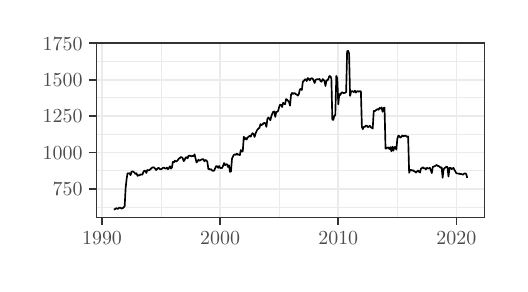
\begin{tikzpicture}[x=1pt,y=1pt]
\definecolor{fillColor}{RGB}{255,255,255}
\path[use as bounding box,fill=fillColor] (0,0) rectangle (170.72, 85.36);
\begin{scope}
\path[clip] (  0.00,  0.00) rectangle (170.72, 85.36);
\definecolor{drawColor}{RGB}{255,255,255}

\path[draw=drawColor,line width= 0.6pt,line join=round,line cap=round,fill=fillColor] (  0.00,  0.00) rectangle (170.72, 85.36);
\end{scope}
\begin{scope}
\path[clip] ( 24.75, 16.77) rectangle (165.22, 79.86);
\definecolor{fillColor}{RGB}{255,255,255}

\path[fill=fillColor] ( 24.75, 16.77) rectangle (165.22, 79.86);
\definecolor{drawColor}{gray}{0.92}

\path[draw=drawColor,line width= 0.3pt,line join=round] ( 24.75, 20.48) --
	(165.22, 20.48);

\path[draw=drawColor,line width= 0.3pt,line join=round] ( 24.75, 33.64) --
	(165.22, 33.64);

\path[draw=drawColor,line width= 0.3pt,line join=round] ( 24.75, 46.81) --
	(165.22, 46.81);

\path[draw=drawColor,line width= 0.3pt,line join=round] ( 24.75, 59.98) --
	(165.22, 59.98);

\path[draw=drawColor,line width= 0.3pt,line join=round] ( 24.75, 73.15) --
	(165.22, 73.15);

\path[draw=drawColor,line width= 0.3pt,line join=round] ( 48.21, 16.77) --
	( 48.21, 79.86);

\path[draw=drawColor,line width= 0.3pt,line join=round] ( 90.89, 16.77) --
	( 90.89, 79.86);

\path[draw=drawColor,line width= 0.3pt,line join=round] (133.58, 16.77) --
	(133.58, 79.86);

\path[draw=drawColor,line width= 0.6pt,line join=round] ( 24.75, 27.06) --
	(165.22, 27.06);

\path[draw=drawColor,line width= 0.6pt,line join=round] ( 24.75, 40.23) --
	(165.22, 40.23);

\path[draw=drawColor,line width= 0.6pt,line join=round] ( 24.75, 53.39) --
	(165.22, 53.39);

\path[draw=drawColor,line width= 0.6pt,line join=round] ( 24.75, 66.56) --
	(165.22, 66.56);

\path[draw=drawColor,line width= 0.6pt,line join=round] ( 24.75, 79.73) --
	(165.22, 79.73);

\path[draw=drawColor,line width= 0.6pt,line join=round] ( 26.87, 16.77) --
	( 26.87, 79.86);

\path[draw=drawColor,line width= 0.6pt,line join=round] ( 69.55, 16.77) --
	( 69.55, 79.86);

\path[draw=drawColor,line width= 0.6pt,line join=round] (112.24, 16.77) --
	(112.24, 79.86);

\path[draw=drawColor,line width= 0.6pt,line join=round] (154.92, 16.77) --
	(154.92, 79.86);
\definecolor{drawColor}{RGB}{0,0,0}

\path[draw=drawColor,line width= 0.6pt,line join=round] ( 31.13, 19.63) --
	( 31.50, 19.74) --
	( 31.82, 20.05) --
	( 32.19, 20.11) --
	( 32.54, 19.84) --
	( 32.90, 20.16) --
	( 33.25, 20.37) --
	( 33.61, 20.21) --
	( 33.97, 20.00) --
	( 34.33, 20.11) --
	( 34.69, 20.48) --
	( 35.04, 20.79) --
	( 35.40, 27.48) --
	( 35.76, 30.75) --
	( 36.10, 32.75) --
	( 36.46, 32.70) --
	( 36.81, 32.75) --
	( 37.18, 32.06) --
	( 37.53, 33.33) --
	( 37.89, 33.43) --
	( 38.25, 33.27) --
	( 38.60, 32.96) --
	( 38.96, 32.48) --
	( 39.32, 32.75) --
	( 39.68, 31.80) --
	( 40.04, 32.06) --
	( 40.37, 31.96) --
	( 40.73, 32.33) --
	( 41.08, 32.33) --
	( 41.44, 32.22) --
	( 41.79, 33.17) --
	( 42.16, 33.70) --
	( 42.52, 33.59) --
	( 42.87, 32.85) --
	( 43.23, 33.96) --
	( 43.58, 33.85) --
	( 43.94, 33.85) --
	( 44.31, 34.17) --
	( 44.63, 34.49) --
	( 44.99, 34.80) --
	( 45.35, 34.91) --
	( 45.71, 34.80) --
	( 46.06, 34.43) --
	( 46.42, 33.91) --
	( 46.78, 34.28) --
	( 47.13, 34.64) --
	( 47.50, 34.64) --
	( 47.85, 34.17) --
	( 48.21, 34.22) --
	( 48.57, 34.38) --
	( 48.90, 34.75) --
	( 49.26, 34.75) --
	( 49.61, 34.54) --
	( 49.97, 34.43) --
	( 50.32, 34.80) --
	( 50.69, 34.22) --
	( 51.05, 34.64) --
	( 51.40, 35.28) --
	( 51.76, 34.43) --
	( 52.11, 34.85) --
	( 52.47, 36.86) --
	( 52.84, 36.70) --
	( 53.18, 37.33) --
	( 53.54, 37.01) --
	( 53.89, 37.12) --
	( 54.25, 37.49) --
	( 54.60, 38.02) --
	( 54.96, 38.23) --
	( 55.33, 38.59) --
	( 55.68, 38.54) --
	( 56.04, 38.17) --
	( 56.39, 37.12) --
	( 56.75, 37.65) --
	( 57.11, 38.44) --
	( 57.44, 38.54) --
	( 57.80, 38.17) --
	( 58.15, 39.12) --
	( 58.52, 39.07) --
	( 58.87, 39.12) --
	( 59.23, 38.81) --
	( 59.59, 39.02) --
	( 59.94, 38.91) --
	( 60.30, 39.60) --
	( 60.65, 38.17) --
	( 61.02, 36.65) --
	( 61.38, 37.07) --
	( 61.71, 37.65) --
	( 62.07, 37.28) --
	( 62.42, 37.49) --
	( 62.78, 37.70) --
	( 63.13, 37.80) --
	( 63.49, 37.86) --
	( 63.86, 37.07) --
	( 64.21, 37.54) --
	( 64.57, 37.38) --
	( 64.92, 36.91) --
	( 65.28, 34.28) --
	( 65.64, 34.33) --
	( 65.97, 34.06) --
	( 66.33, 34.22) --
	( 66.68, 33.70) --
	( 67.05, 33.64) --
	( 67.40, 33.70) --
	( 67.76, 34.64) --
	( 68.12, 35.33) --
	( 68.47, 35.28) --
	( 68.83, 34.70) --
	( 69.19, 35.38) --
	( 69.55, 34.64) --
	( 69.91, 34.70) --
	( 70.25, 34.64) --
	( 70.61, 35.43) --
	( 70.96, 36.44) --
	( 71.32, 35.70) --
	( 71.67, 35.96) --
	( 72.04, 36.01) --
	( 72.40, 35.01) --
	( 72.75, 35.64) --
	( 73.11, 33.27) --
	( 73.46, 33.38) --
	( 73.83, 38.02) --
	( 74.19, 38.81) --
	( 74.51, 39.44) --
	( 74.88, 39.54) --
	( 75.23, 39.44) --
	( 75.59, 39.86) --
	( 75.94, 39.44) --
	( 76.30, 39.54) --
	( 76.66, 39.28) --
	( 77.02, 41.18) --
	( 77.38, 40.54) --
	( 77.73, 40.70) --
	( 78.09, 45.97) --
	( 78.45, 45.02) --
	( 78.78, 45.49) --
	( 79.14, 44.97) --
	( 79.49, 45.70) --
	( 79.86, 45.97) --
	( 80.21, 46.28) --
	( 80.57, 45.97) --
	( 80.93, 46.76) --
	( 81.28, 47.23) --
	( 81.64, 46.92) --
	( 81.99, 45.86) --
	( 82.36, 47.18) --
	( 82.72, 47.97) --
	( 83.05, 48.60) --
	( 83.41, 48.86) --
	( 83.76, 49.23) --
	( 84.12, 50.50) --
	( 84.47, 50.13) --
	( 84.83, 50.39) --
	( 85.20, 50.76) --
	( 85.55, 51.02) --
	( 85.91, 50.76) --
	( 86.26, 49.50) --
	( 86.62, 52.39) --
	( 86.98, 52.92) --
	( 87.32, 52.45) --
	( 87.69, 51.92) --
	( 88.04, 53.34) --
	( 88.40, 54.34) --
	( 88.75, 54.97) --
	( 89.11, 55.08) --
	( 89.47, 53.13) --
	( 89.82, 54.92) --
	( 90.19, 54.92) --
	( 90.54, 55.40) --
	( 90.90, 56.82) --
	( 91.26, 57.56) --
	( 91.59, 57.45) --
	( 91.95, 56.71) --
	( 92.30, 58.24) --
	( 92.66, 57.82) --
	( 93.01, 57.71) --
	( 93.38, 59.56) --
	( 93.74, 59.35) --
	( 94.09, 58.92) --
	( 94.45, 58.50) --
	( 94.80, 57.19) --
	( 95.16, 61.03) --
	( 95.53, 61.77) --
	( 95.85, 61.40) --
	( 96.22, 61.72) --
	( 96.57, 61.66) --
	( 96.93, 61.29) --
	( 97.28, 61.14) --
	( 97.64, 60.82) --
	( 98.00, 61.40) --
	( 98.35, 63.03) --
	( 98.72, 63.24) --
	( 99.07, 62.82) --
	( 99.43, 65.82) --
	( 99.79, 66.14) --
	(100.12, 66.61) --
	(100.48, 66.72) --
	(100.83, 66.09) --
	(101.19, 67.14) --
	(101.55, 66.98) --
	(101.91, 66.30) --
	(102.27, 66.88) --
	(102.62, 67.09) --
	(102.98, 66.98) --
	(103.33, 66.25) --
	(103.70, 65.35) --
	(104.06, 66.56) --
	(104.40, 66.67) --
	(104.76, 66.77) --
	(105.11, 66.72) --
	(105.47, 66.83) --
	(105.82, 66.09) --
	(106.18, 65.82) --
	(106.55, 66.77) --
	(106.90, 66.56) --
	(107.26, 66.04) --
	(107.61, 64.30) --
	(107.97, 66.35) --
	(108.33, 66.25) --
	(108.66, 66.93) --
	(109.02, 67.88) --
	(109.37, 67.83) --
	(109.74, 66.98) --
	(110.09, 52.13) --
	(110.45, 52.03) --
	(110.81, 53.45) --
	(111.16, 53.76) --
	(111.53, 67.93) --
	(111.88, 67.14) --
	(112.24, 57.66) --
	(112.60, 61.35) --
	(112.93, 61.03) --
	(113.29, 61.72) --
	(113.64, 62.03) --
	(114.00, 61.77) --
	(114.35, 61.72) --
	(114.72, 61.87) --
	(115.08, 62.08) --
	(115.43, 76.83) --
	(115.79, 76.99) --
	(116.14, 76.04) --
	(116.50, 60.72) --
	(116.87, 62.30) --
	(117.19, 62.45) --
	(117.56, 62.30) --
	(117.91, 62.08) --
	(118.27, 62.61) --
	(118.62, 61.87) --
	(118.98, 62.35) --
	(119.34, 62.40) --
	(119.69, 62.19) --
	(120.06, 62.45) --
	(120.41, 62.35) --
	(120.77, 49.44) --
	(121.13, 48.71) --
	(121.47, 49.55) --
	(121.83, 49.50) --
	(122.18, 49.97) --
	(122.55, 49.97) --
	(122.90, 49.39) --
	(123.26, 49.60) --
	(123.62, 49.92) --
	(123.97, 49.39) --
	(124.33, 49.18) --
	(124.68, 48.92) --
	(125.05, 55.24) --
	(125.41, 55.19) --
	(125.74, 55.50) --
	(126.10, 55.71) --
	(126.45, 55.98) --
	(126.81, 55.71) --
	(127.16, 56.34) --
	(127.52, 56.13) --
	(127.89, 56.55) --
	(128.24, 54.97) --
	(128.60, 56.29) --
	(128.95, 56.50) --
	(129.31, 41.65) --
	(129.67, 41.75) --
	(130.00, 42.02) --
	(130.36, 42.07) --
	(130.71, 41.49) --
	(131.08, 42.18) --
	(131.43, 40.70) --
	(131.79, 42.39) --
	(132.15, 40.91) --
	(132.50, 42.18) --
	(132.86, 42.28) --
	(133.22, 41.28) --
	(133.58, 45.28) --
	(133.94, 46.34) --
	(134.27, 46.18) --
	(134.63, 45.65) --
	(134.98, 45.81) --
	(135.34, 46.39) --
	(135.69, 46.13) --
	(136.05, 46.23) --
	(136.42, 46.34) --
	(136.77, 46.18) --
	(137.13, 45.86) --
	(137.48, 46.07) --
	(137.84, 32.91) --
	(138.21, 33.96) --
	(138.54, 33.91) --
	(138.91, 33.70) --
	(139.26, 33.85) --
	(139.62, 33.49) --
	(139.97, 33.33) --
	(140.33, 33.01) --
	(140.69, 33.43) --
	(141.05, 33.75) --
	(141.41, 33.33) --
	(141.76, 33.01) --
	(142.12, 34.43) --
	(142.48, 34.64) --
	(142.81, 34.91) --
	(143.17, 34.49) --
	(143.52, 34.59) --
	(143.88, 34.12) --
	(144.24, 34.70) --
	(144.60, 34.54) --
	(144.96, 34.49) --
	(145.31, 34.70) --
	(145.67, 33.91) --
	(146.02, 32.80) --
	(146.39, 35.01) --
	(146.75, 35.22) --
	(147.08, 35.28) --
	(147.44, 35.54) --
	(147.79, 35.75) --
	(148.15, 35.38) --
	(148.50, 35.38) --
	(148.86, 35.12) --
	(149.23, 34.70) --
	(149.58, 34.91) --
	(149.94, 31.12) --
	(150.29, 34.17) --
	(150.65, 34.64) --
	(151.01, 34.85) --
	(151.34, 35.22) --
	(151.70, 34.91) --
	(152.05, 31.59) --
	(152.42, 34.64) --
	(152.77, 34.80) --
	(153.13, 34.22) --
	(153.49, 34.43) --
	(153.84, 34.70) --
	(154.20, 33.96) --
	(154.55, 33.43) --
	(154.92, 32.70) --
	(155.28, 32.70) --
	(155.62, 32.59) --
	(155.98, 32.64) --
	(156.33, 32.43) --
	(156.69, 32.48) --
	(157.04, 32.33) --
	(157.41, 32.27) --
	(157.77, 32.70) --
	(158.12, 32.70) --
	(158.48, 32.43) --
	(158.83, 31.06);
\definecolor{drawColor}{gray}{0.20}

\path[draw=drawColor,line width= 0.6pt,line join=round,line cap=round] ( 24.75, 16.77) rectangle (165.22, 79.86);
\end{scope}
\begin{scope}
\path[clip] (  0.00,  0.00) rectangle (170.72, 85.36);
\definecolor{drawColor}{gray}{0.30}

\node[text=drawColor,anchor=base east,inner sep=0pt, outer sep=0pt, scale=  0.72] at ( 19.80, 24.60) {750};

\node[text=drawColor,anchor=base east,inner sep=0pt, outer sep=0pt, scale=  0.72] at ( 19.80, 37.76) {1000};

\node[text=drawColor,anchor=base east,inner sep=0pt, outer sep=0pt, scale=  0.72] at ( 19.80, 50.93) {1250};

\node[text=drawColor,anchor=base east,inner sep=0pt, outer sep=0pt, scale=  0.72] at ( 19.80, 64.10) {1500};

\node[text=drawColor,anchor=base east,inner sep=0pt, outer sep=0pt, scale=  0.72] at ( 19.80, 77.27) {1750};
\end{scope}
\begin{scope}
\path[clip] (  0.00,  0.00) rectangle (170.72, 85.36);
\definecolor{drawColor}{gray}{0.20}

\path[draw=drawColor,line width= 0.6pt,line join=round] ( 22.00, 27.06) --
	( 24.75, 27.06);

\path[draw=drawColor,line width= 0.6pt,line join=round] ( 22.00, 40.23) --
	( 24.75, 40.23);

\path[draw=drawColor,line width= 0.6pt,line join=round] ( 22.00, 53.39) --
	( 24.75, 53.39);

\path[draw=drawColor,line width= 0.6pt,line join=round] ( 22.00, 66.56) --
	( 24.75, 66.56);

\path[draw=drawColor,line width= 0.6pt,line join=round] ( 22.00, 79.73) --
	( 24.75, 79.73);
\end{scope}
\begin{scope}
\path[clip] (  0.00,  0.00) rectangle (170.72, 85.36);
\definecolor{drawColor}{gray}{0.20}

\path[draw=drawColor,line width= 0.6pt,line join=round] ( 26.87, 14.02) --
	( 26.87, 16.77);

\path[draw=drawColor,line width= 0.6pt,line join=round] ( 69.55, 14.02) --
	( 69.55, 16.77);

\path[draw=drawColor,line width= 0.6pt,line join=round] (112.24, 14.02) --
	(112.24, 16.77);

\path[draw=drawColor,line width= 0.6pt,line join=round] (154.92, 14.02) --
	(154.92, 16.77);
\end{scope}
\begin{scope}
\path[clip] (  0.00,  0.00) rectangle (170.72, 85.36);
\definecolor{drawColor}{gray}{0.30}

\node[text=drawColor,anchor=base,inner sep=0pt, outer sep=0pt, scale=  0.72] at ( 26.87,  6.89) {1990};

\node[text=drawColor,anchor=base,inner sep=0pt, outer sep=0pt, scale=  0.72] at ( 69.55,  6.89) {2000};

\node[text=drawColor,anchor=base,inner sep=0pt, outer sep=0pt, scale=  0.72] at (112.24,  6.89) {2010};

\node[text=drawColor,anchor=base,inner sep=0pt, outer sep=0pt, scale=  0.72] at (154.92,  6.89) {2020};
\end{scope}
\end{tikzpicture}

        \caption{Disponibilità mensile di serie in SCIA}
      \end{figure}
    \end{column}
  \end{columns}
\end{frame}